\documentclass[oneside,10pt]{book}
\usepackage{cdtBook}
\usepackage{usecases}
\usepackage{amsmath}
\usepackage{hyperref}
\usepackage{longtable}

\usepackage{listings}
\lstset{%
breaklines=true
showspaces=false
showstringspaces=false
showtabs=false
}



\title{Trabajo Terminal 2013-B017}
\subtitle{Sistema de an\'alisis de texto mediante reconocimiento de patrones. Caso de estudio: \textit{Online grooming}}
\author{Guerrero Madrigal Andr\'es Emanuel, Hern\'andez Hern\'andez Santos, Ruiz D\'iaz Anah\'i}
%\organization{Escuela Superior de Cómputo, IPN}



%%%%%%%%%%%%%%%%%%%%%%%%\usepackage{longtable}%%%%%%%%%%%%%%%%%%%%%%%%%%%%%%%%%%%%%%%%

\begin{document}

\begin{titlepage}


%\begin{center}
%\begin{tabular}{r c}
%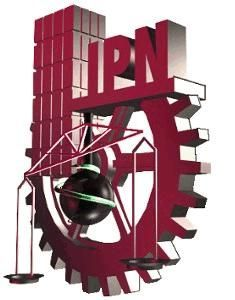
\includegraphics[scale=.3]{images/ipn.jpg} & \LARGE \textbf{Instituto Polit\'ecnico Nacional} & 
\includegraphics[scale=.3]{images/escom.jpg} \\
%& \Large \textbf{Escuela Superior de C\'omputo} &
%\end{tabular}
%\end{center}

\begin{center}
\begin{tabular}{r c l}
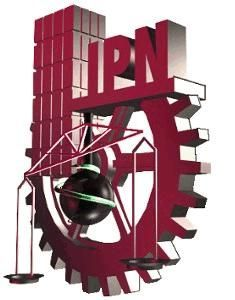
\includegraphics[scale=.10]{images/ipn.jpg} & \huge \textbf{INSTITUTO POLITÉCNICO NACIONAL} & 
\includegraphics[scale=.25]{images/escom.jpg}\\ 
& \Large \textbf{ESCUELA SUPERIOR DE CÓMPUTO}
\end{tabular}
\end{center}


\vspace{1.5cm}
\begin{center}
\large Trabajo Terminal: \linebreak

\large \textbf{``Sistema de Detección de Intrusos para ataques Cross-Site Scripting''} \linebreak
\large 2016-B089

\end{center}

\vspace{1.5cm}

\begin{center}
Presentan: \linebreak
\textbf{Fonseca Casao Sergio Israel} \linebreak
\textbf{Israel García Ramírez} \linebreak
\end{center}

\vspace{1.5cm}

El presente documento se encuentran los temas relacionados al desarrollo del Trabajo Terminal I cuyo objetivo es el desarrollo de un sistema de detección de intrusos que se especifique en la detección de ataques Cross-Site Scripting (XSS) mediante la aplicación de aprendizaje máquina. Este sistema pretende servir como herramienta capaz de detectar y alertar a los administradores de los servidores de un ataque XSS en curso y almacenar los datos necesarios para su posterior análisis.\linebreak

\textbf{Palabras Clave}:  Aprendizaje Automático, Cross-Site Scripting, Lenguajes Regulares, Sistema de Detección de Intrusos.

\vspace{1.5cm}
 
\begin{center}


Directores: \linebreak
\textbf{ M. en C. Ramírez Morales Mario Augusto, M. en E. Saucedo Delgado Rafael Norman}

\end{center}





\end{titlepage}


\thispagestyle{empty}

\frontmatter
\tableofcontents
\frontmatter
\listoffigures % indice de figuras
\frontmatter
\listoftables % indice de tablas

\mainmatter

%=========================================================
\chapter{Antecedentes}
%---------------------------------------------------------
\section{Introducción}

La seguridad informática ha sido y actualmente es un sector en el cual, empresas importantes de gran prestigio gastan cientos de
millones de dólares para protegerse al estar conectados a una red \cite{uno}, tal es la preocupación que a nivel mundial se registró una
inversión en la seguridad informática de 75 billones de dólares en 2015 \cite{dos}, mientras que, tanto chicas como medianas empresas
suelen gastan un mínimo relacionado a este tema. En la actualidad, con la era de la revolución tecnológica por la que se está
pasando, las empresas se han visto obligadas a contratar nueva tecnología para su producción, publicidad y/o servicios conectada al
mundo de la Internet. Las empresas al estar conectadas a la Internet, están conectadas a millones de usuarios con cientos de
posibilidades de acceso a los servicios de las empresas.\\

Cuando los usuarios se conectan a la red de Internet, están conectados todos los usuarios de la misma simultáneamente, esto
conlleva un alto riesgo de inseguridad. Para tratar de disminuir el impacto provocado por amenazas informáticas, existen
programas de computadora enfocados a detectar y proteger a los usuarios de la red contra los impactos provocados por las
amenazas \cite{tres}.\\

Hoy en día, existen diversos tipos de amenazas en la red, algunas son muy conocidas como virus informáticos que son diseñados
para infectar archivos, pero no sólo existen ese tipo de amenazas diseñadas cierta forma con una actuación “automatizada”.
También existen las amenazas humanas o conocidos como Piratas informáticos, los cuáles, por medio de diversas técnicas de
vulneración, pueden infectar, tomar el control o incluso obtener información o privilegios de computadoras o servidores con el fin
de aprender o poner en práctica nuevas técnicas de vulneración, vender la información obtenida en el mercado negro o inclusive
realizar un daño directo a los archivos o computadora objetivo \cite{cuatro}\cite{cinco}.\\

Con el incremento de nuevos servicios web en Internet, se han creado y desarrollado diversos tipos de ataques hacia los servidores
que proporcionan estos servicios. En los últimos años han ido en incremento los ataques web, aunque los que han tenido un mayor
crecimiento y un gran impacto a nivel global, son los ataques tipo Cross-Site Scripting (de ahora en adelante XSS) \cite{seis}.

\subsection{Servicios de Seguridad}

Es cuya función principal es mejorar la seguridad de un sistema de información y el flujo de información que pasa a través de una organización. Los servicios  de seguridad están orientados a evitar ataques de informáticos haciendo uso de distintos controles de seguridad para proveer el servicio. Cada control de seguridad está diseñado para realizar una función determinada dependiendo del servicio de seguridad que se desee otorgar.\\

Los servicios de seguridad se dividen en seis clasificaciones: \\

\begin{itemize}

	\item Disponibilidad: Es un requerimiento destinado a asegurar que el sistema trabaja apropiadamente y el servicio no deniega a usuarios autorizados. Este servicio protege contra: 
		\begin{itemize}
		\item Intentos intencionales o accidentales de:
			\begin{itemize}
			\item eliminación no autorizada de datos o
			\item de lo contrario causar una denegación de servicio o datos.
			\end{itemize}
		\item Intentos para usar el sistema o datos para propósitos no autorizados.
		\end{itemize}
	La disponibilidad es frecuentemente es el principal objetivo de seguridad de una organización.
	
	\item Integridad: Tiene dos facetas: 
		\begin{itemize}
			\item Integridad de datos (la propiedad de que los datos no han sido alterados en un manejo no autorizado) o
			\item Integridad del sistema (la calidad que tiene un sistema al realizar la función deseada de manera intacta, libre de manipulación no autorizada).
		\end{itemize}
	La integridad es comúnmente el objetivo más importante dentro de una organización después de la disponibilidad.
	
	\item Confidencialidad: Consiste en que información dentro del sistema de una organización no sea accesada por personal no autorizado.
	Por diversas razones, aún se pone la confidencialidad debajo de la disponibilidad e integridad en términos de importancia. Pero a pesar de esto, para algunos sistemas, de autenticación, por ejemplo, la confidencialidad es el objetivo más importante a considerar. 
	
	\item No repudio: Consiste en identificar al responsable de una acción (un ataque, por ejemplo) hacia un sistema, responsabilizándolo por los actos y sin la posibilidad de que éste niegue los hechos.
	
	\item Autenticación: Es un requerimiento que consiste la identificación de un personal para que no pueda ser suplantado, y así acceder a cierta información contenida en un sistema.

\end{itemize}


\subsection{Controles de Seguridad}

Los controles de seguridad proveen un rango comprensivo de contra-medidas para organizaciones y sistemas de información. Los controles de seguridad son diseñados para ser tecnologías neutrales tal manera que se centre en las contra-medidas fundamentales necesitadas para proteger la información de la organización durante el procesamiento, almacenamiento o su transmisión \cite{nist53}. La implementación de los controles de seguridad dependen al nivel de protección que se desee tener en un sistema. Las buenas prácticas de seguridad hacen mención que para tener una buena protección en un sistema u organización, se deben de emplear los controles de seguridad en conjunto, haciendo referencia que se deben de emplear varios de estos controles para así complementar brechas de seguridad que se contengan en los controles.\\

Mencionando algunos controles más populares empleados, tenemos los siguientes: \\

\begin{itemize}

	\item Cortafuegos: Su función es delimitar el área perimetral de la red filtrando el flujo de red, tanto de entrada como de salida e incluso entre la comunicación de diferentes áreas dentro de la misma red. Se tiene tres categorías, los cortafuegos de paquete, de estado y de aplicación, donde su modo de operación varía en que el primero sólo se fija en el algunos campos del encabezado de los paquetes de red, el segundo hace un análisis más profundo del encabezado y el último hace un análisis en el \textit{payload}\footnote{Los datos esenciales que es llevada dentro de un paquete de red y otra unidad de transmisión} del paquete de red.
	
	\item Proxy: Es una entidad que funciona como intermediario entre la comunicación entre redes de una organización.
	
	\item Antivirus: Programa que tiene como finalidad detectar código malicioso dentro de los sistemas de lo cuáles se encarga de analizar.
	
	\item Detección de Intrusos: Programas que se encargan de hacer un monitoreo de las entidades de las cuáles se encarga.
	
	\item Honey Pots (por su nombre en inglés): Entidad que se encarga se ser un señuelo específicamente diseñado para atraer atacantes y\/o ver el comportamiento de programas maliciosos, con la finalidad de utilizarse como fuente para estudiar las nuevas formas de intrusión.

\end{itemize} 


\pagebreak
%---------------------------------------------------------
\section{Descripci\'on del problema}

Un ataque XSS ocurre cuando un atacante es capaz de inyectar un script, normalmente JavaScript, en la salida de una aplicación
web de forma que se ejecuta en el navegador del cliente. Los ataques se producen principalmente por validar incorrectamente datos
de usuario, y se suelen inyectar mediante un formulario web o mediante un enlace alterado.\\

Existen tres tipos de ataques XSS: \\

\begin{itemize}
	\item XSS persistente o directo: este tipo de ataque consiste en embeber código HTML peligroso en sitios que lo permitan por
medio de etiquetas \textit{<script>} o \textit{<iframe>}. Es la más grave de todas ya que el código se queda implantado en la web de
manera interna y es ejecutado al abrir la aplicación web.\\

	\item XSS reflejado: en este tipo de ataque el código malicioso no queda almacenado en el servidor sino que se pasa
directamente a la víctima. Es la forma más habitual de XSS. El ataque se lanza desde una fuente externa como un correo
aparentemente inofensivo, un mensaje de chat u otro sitio web \cite{siete}.\\

	\item XSS basado en DOM: es una variable de XSS persistente y reflejado. En un ataque XSS basado en DOM, la cadena maligna no es realmente analizada por el navegador de la victima hasta que el JavaScript legítimo de la página web es ejecutado. Estos códigos son ejecutados del lado
del cliente, por lo que los filtros utilizados en el servidor no funcionan para este tipo de vulnerabilidades.\\
\end{itemize}

A la hora de lanzar un ataque de este tipo, los atacantes pueden utilizar varios tipos de inyección de código distinto. Los más utilizados son:\\

\begin{itemize}
	\item Inyección en un formulario: se trata del ataque más sencillo. Consiste en inyectar código en un formulario que después al
enviarlo al servidor, será incluido en el código fuente de alguna página. Una vez insertado en el código fuente, cada vez
que se cargue la página se ejecutará el código insertado en ella.

	\item Inyección por medio de elementos: en este tipo de sistema de inyección de código se utiliza cualquier elemento que viaje
entre el navegador y la aplicación, como pueden ser los atributos usados en las etiquetas HTML utilizadas en el diseño de
la página.

	\item Inyección por medio de recursos: Aparte de los elementos en la URL y los formularios, hay otras formas en la que se
puede actuar como son las cabeceras HTTP. Estas cabeceras son mensajes con los que se comunican el navegador y el
servidor. Aquí entran en juego las \textit{cookies}\footnote{Una cookie es un pequeño elemento de información que un servidor Web envía al navegador al visitar ciertas páginas web y que ambos comparten cada que este navegador vuelve a visitar \cite{cookie}.} y las sesiones \cite{ocho}.\\
\end{itemize}

Los daños potenciales que pueden causar un ataque XSS, pueden afectar tanto a los servidores en donde está contenida la
aplicación web o pueden provocar serios problemas para el usuario final, éstos pueden varían en el grado de impacto, pueden ir
desde una molestia para el usuario hasta un compromiso completo de la cuenta del mismo. Uno de los efectos más graves de los
ataques XSS implica la divulgación de cookies de sesión del usuario, lo que permite a un atacante secuestrar la sesión del usuario y
tomar control total de la cuenta. Otros ataques dañinos incluyen la divulgación de los archivos de los usuarios finales, la instalación
de programas dañinos para el equipo del usuario final, redirigir al usuario a otra página o sitio web con fines malicioso, o modificar
la presentación de los contenidos \cite{nueve}. Los ataques XSS explotan vulnerabilidades no en el navegador del usuario, sino en las
aplicaciones Web de terceros a las que accede el usuario. En este tipo de ataque el navegador no puede distinguir entre el contenido
que un usuario haya podido incluir en una petición Web, y el contenido inyectado a través de un ataque XSS \cite{diez}.\\

Se han desarrollado nuevas tecnologías que utilizan diferentes técnicas para poder detectar, contrarrestar y protegerse de los ataques tipo XSS \cite{once}, algunas de esas tecnologías son aplicadas en Cortafuegos de Aplicaciones Web (WAFs, por sus siglas en inglés), los Sistemas de Detección de Intrusos (IDSs, por sus siglas en inglés) e inclusive, las mismas empresas desarrolladoras de antivirus, han integrado nuevos módulos en sus sistemas en contra de este tipo de ataques \cite{doce}.\\

Aunque se tiene registros de los problemas causados y el incremento que ha tenido este tipo de ataque, el principal objetivo de las tecnologías que se lanzan al mercado no es completamente enfocado a este ataque. Tal hecho provoca que al realizar auditorías de las herramientas en ésta parte de vulnerabilidades, se detecten fallos en el sistema, tales como falsos positivos o falsos negativos.\\
%---------------------------------------------------------
\section{Soluci\'on propuesta}
El presente Trabajo Terminal implementa un sistema que mediante reconocimiento de patrones, aprendizaje m\'aquina y miner\'ia de datos; sea capaz de analizar y clasificar texto en el idioma espa\~nol a partir de un conjunto de datos estad\'isticos. Aplicado al caso de estudio \textit{online grooming.}

% con el objetivo de poder determinar si una conversaci\'on es peligrosa o no. 
%Con el desarrollo de este trabajo pretendemos, si bien no terminar con el \textit{grooming}, brindar una herramienta la cual ayude a prevenir posibles ataques a menores por parte de adultos malintencionados dentro de la red. \\ 
%---------------------------------------------------------
\section{Estado del arte}
Anteriormente se han definido brevemente varios conceptos sobre los que se hablará en el resto del documento. Estos conceptos sirven para dar una idea muy básica al lector.\\

En la presente sección, en la Tabla \ref{table:EdoArte} se entra en profundidad a definir el estado del arte y las caracteríticas mas relevantes de los IDS que existen actualmente en el mercado.\\


\begin{table}[h]
	\begin{center}
		\begin{tabular}{|l|p{75mm}|l|l|l|l|}
		\hline
		Nombre & Descripción & Tipo & Año & Lugar de desarrollo & Escrito en \\
		\hline
	    SNORT & Se trata de un sistema basado en red que monitoriza todo un dominio de colisión y funciona detectando usos indebidos. Dispone de un lenguaje de creación de reglas en el que se pueden definir los patrones que se utilizarán a hora de monitorizar el sistema. Además, ofrece una serie de reglas y filtros ya predefinidos que se pueden ajustar durante su instalación y configuración. & Open Source & 1998 & Cisco Systems & C \\
		\hline
	    Suricata & Es un motor de detección de amenazas de red, maduro, rápido y robusto, de código abierto y gratuito. Es capaz de detectar intrusos en tiempo real, prevención de intrusiones en línea, supervisión de seguridad de red y procesamiento offline de pcap. & Open Source & 2009 & OISF & C \\
		\hline
	    Bro & Es un sistema de detección de intrusiones para UNIX/Linux que analiza el tráfico de red en busca de actividad sospechosa. Su característica principal es que sus reglas de detección están basados en su lenguaje nativo que supone políticas (policies) que son las encargadas de detectar, generar logs o eventos y acciones a nivel de sistema operativo. & Open Source & 2005 & ICSI and NCSA & C++ \\
		\hline
	    Security Onion & Es un sistema que consiste en varias de las tecnologías de código abierto de mencionadas anteriormente trabajando en concierto entre sí. La plataforma ofrece una completa detección de intrusos, monitoreo de seguridad de red y administración de registros combinando lo mejor de Snort, Suricata, Bro, así como otras herramientas como Sguil, Squert, Snorby, ELSA, Xplico, entre otras. & Open Source & 2010 & \- & \- \\
		\hline
		\end{tabular}
		\caption{Comparativa de IDSs en el mercado}
		\label{table:EdoArte}
	\end{center}
\end{table}





Existen además otros sistemas como lo son: Kismet, SmartDefense, Symantec Network Security 7100, Cisco Secure IDS 4230. \\

%\cfinput{Antecedentes/Objetivo}
\subsection{Justificación de los Sistemas de Detección de Intrusos}

Los sistemas de detección de intrusos (IDS por sus siglas en inglés) es un control de seguridad que debe ser implementado junto con otros controles de seguridad para fortalecer y\/o complicar la acción de una contra-parte, como es el caso de un \textit{cortafuegos}\footnote{Un cortafuegos o \textit{firewall}, por su nombre en inglés, son dispositivos o programas que controlan el flujo del tráfico de red entre redes o computadoras que emplean diferentes posturas de seguridad\cite{nist41}.}. La implementación de estos dos controles de seguridad son comúnmente empleados ya que el trabajo del cortafuegos el filtrar el tráfico de la red con base a un análisis de filtrado de paquetes o un filtrado de estado. Así, los IDSs reciben tráfico filtrado y reconocido para su análisis de acuerdo a diversos criterios dependiendo de la taxonomía implementada (que se definirá después). 
\\

Existen hoy en día entidades que emplean IDS dentro de los cortafuegos, ya que son la primera línea de seguridad defensiva de una entidad, con el objetivo de complementar su sistema de filtrado, y así ser más eficiente y oportuno durante un ataque o intento de intrusión. Pero dicha implementación no es que sea mejor que una de forma separada entre controles, más bien radica en otros factores como la cantidad de dispositivos existentes en la entidad que lo va a implementar, la cantidad de información que va a procesar y principalmente los recursos monetarios disponibles de la entidad, haciendo mención también que al juntar estos controles, el tiempo de procesamiento de los datos dependería mucho del hardware del dispositivo, así haciendo dependiente el flujo sin retardos de la red al dispositivo. También hay que tener en consideración que si la implementación de diferentes controles de seguridad se hace en un mismo dispositivo, existe un mayor riesgo de que si el dispositivo falla o es comprometido, la entidad pueda sufrir un ataque o una intrusión. 
\\
%=========================================================
\chapter{Marco Te\'orico}
%\cfinput{MarcoTeorico/casodeestudio}
\section{Miner\'ia de texto}

\section{Lenguaje natural}
El lenguaje se considera como un mecanismo que nos permite hablar y entender. Los lenguajes naturales, es decir, el ingl\'es, el franc\'es, el espa\~nol, etc. son una herramienta genuina para la comunicaci\'on entre los seres humanos, ya sea en forma oral o escrita.
Actualmente, el avance tecnol\'ogico en los medios de comunicaci\'on impresos y electr\'onicos nos permite obtener grandes vol\'umenes de informaci\'on en forma escrita. La mayor\'ia de esta informaci\'on se presenta en forma de textos en lenguajes naturales. Toda esa informaci\'on contenida en los textos es muy importante ya que permite analizar, comparar, entender el entorno en el que vive el ser humano.
Sin embargo, se presentan dificultades por la imposibilidad humana de manejar esa enorme cantidad de textos. Entre las herramientas que ayudan en las tareas diarias, la computadora es, hoy en d\'ia, una herramienta indispensable para el procesamiento de grandes vol\'umenes de datos. Pero todav\'ia no se logra que una m\'aquina al capturar una colecci\'on de textos los comprenda suficientemente bien; por ejemplo, para que pueda aconsejar qu\'e hacer en determinado momento bas\'andose en toda la informaci\'on proporcionada, para que pueda responder a preguntas acerca de los temas contenidos en esa informaci\'on pero no expl\'icitamente descritos, o para que pueda elaborar un resumen de la informaci\'on.
Para lograr esta enorme tarea de procesamiento de lenguaje natural por computadora, analizando oraci\'on por oraci\'on para obtener el sentido de los textos, es necesario conocer las reglas y los principios bajo los cuales funciona el lenguaje, a fin de reproducirlos y adecuarlos a la computadora, incluyendo posteriormente el procesamiento de lenguaje natural en el proceso general del conocimiento y el razonamiento.
El estudio del lenguaje, est\'a relacionado con diversas disciplinas. De entre ellas, la Ling\"u\'istica General es el estudio te\'orico que se ocupa de los m\'etodos de investigaci\'on y de las cuestiones comunes a las diversas lenguas. Esta disciplina a su vez comprende una multitud de aspectos (temporales, metodol\'ogicos, sociales, culturales, de aprendizaje, etc.). Los aspectos metodol\'ogicos y de aplicaci\'on brindan los principios y las reglas necesarios en el procesamiento de textos.
Los principios y las reglas de la ling\"u\'istica general, aunados a los m\'etodos de la computaci\'on forman la Ling\"u\'istica Computacional. Esta es la \'area dentro de la cu\'al se han desarrollado y discutido muchos formalismos adecuados para la computadora a fin de reproducir el funcionamiento del lenguaje con la finalidad de extraer sentido a partir de textos y viceversa, transformando los conceptos de sentidos espec\'ificos a los correspondientes textos correctos. \cite{cic}
\section{Procesamiento del lenguaje natural}

El t\'ermino "Procesamiento del lenguaje natural" (PLN) hace referencia a las t\'ecnicas de tratamiento del lenguaje y su aplicaci\'on en las diversas \'areas por medio de m\'etodos computacionales.  \cite{elprofesionaldelainformacion}

El PLN es un \'area de investigaci\'on en continuo desarrollo, es aplicado en la actualidad para la realizaci\'on de diversas actividades como son: traducci\'on autom\'atica, sistemas de recuperaci\'on de informaci\'on, elaboraci\'on autom\'atica de res\'umenes, etc\'etera.  \cite{elprofesionaldelainformacion}

Si bien es cierto que la evoluci\'on de dicha \'area la posiciona para liderar una nueva dimensi\'on en las aplicaciones inform\'aticas del futuro, la complejidad impl\'icita en el tratamiento del lenguaje tiene sus limitaciones en los resultados.

Podemos definir el PLN como el reconocimiento y utilizaci\'on de la informaci\'on expresada en lenguaje humano a trav\'es del uso de sistemas inform\'aticos. En su estudio intervienen diferentes disciplinas: la ling\"u\'istica, ingenier\'ia inform\'atica, filosof\'ia, matem\'aticas y psicolog\'ia. \cite{elprofesionaldelainformacion}

Es importante el estudio del lenguaje para determinar el uso que implica \'este en diferentes tareas y de esta manera poder moldear el conocimiento de una manera adecuada. \cite{elprofesionaldelainformacion}

Es necesario tener en cuenta dos puntos: El primero tener en cuenta el problema de representaci\'on ling\"u\'istica para el cual se desea aplicar dicha t\'ecnica. Y en segunda el problema de tratamiento mediante recursos inform\'aticos.
\pagebreak

 %\cite{elprofesionaldelainformacion}

%\begin{thebibliography}{99}

%\bibitem{elprofesionaldelainformacion} Sosa, Eduardo. "Procesamiento del lenguaje natural: revisi\'on del estado actual, bases te\'oricas y aplicaciones (Parte I)". El Profesional de la Informaci\'on. N.p., Jan. 1997. Web. 6 Apr. 2014. 
%\end{thebibliography}
\section{An\'alisis morfol\'ogico}

En el espa\~nol existe una enorme cantidad de palabras que pueden desempe\~nar diferentes funciones gramaticales. El an\'alisis de un texto producir\'a una gran multiplicidad de combinaciones posibles.

El an\'alisis morfol\'ogico consiste en la detecci\'on de la relaci\'on que se establece entre las unidades m\'inimas que forman una palabra: reconocimiento de sufijos o prefijos. Este nivel de an\'alisis  mantiene una estrecha relaci\'on con el l\'exico. \cite{elprofesionaldelainformacion}

El an\'alisis morfol\'ogico consiste en determinar la forma, clase o categor\'ia gramatical de cada palabra de una oraci\'on. \cite{morfo}

\begin{center}

\begin{table}[h]

\begin{tabular}{|l|p{75mm}|l|l|p{50mm}|}

\hline

Sustantivo &  Masculino o Femenino, Singular o Plural, Com\'un o Propio, Concreto o Abstracto, Individual o Colectivo. Si lleva Sufijo, puede dar idea de aumento, de disminuci\'on o de desprecio (Aumentativo, Diminutivo o Despectivo). \\
\hline

Adjetivo & Masculino o Femenino, Singular o Plural, Determinativo o Calificativo; Demostrativo, Posesivo, Numeral, Relativo o Indefinido. Grado Positivo, Grado Comparativo o Grado Superlativo. Cuando portan Sufijo pueden considerarse como Aumentativos, Diminutivos o Despectivos.\\
\hline
Verbo & Persona, Singular o Plural, Tiempo, Modo, Voz, Conjugaci\'on, Forma Personal o No Personal. \\
\hline
Adverbio & Lugar, Modo, Tiempo, Cantidad, Intensidad, etc. Si modifica al verbo, o a otro adverbio. \\
\hline
Pronombre & Masculino o Femenino, Singular o Plural, Determinado o Indeterminado.\\
\hline
Art\'iculo & Lugar, Modo, Tiempo, Cantidad, Intensidad, etc. Si modifica al verbo, o a otro adverbio. \\
\hline
Conjunci\'on & Coordinada o Subordinada; Copulativa, Adversativa, Distributiva o Disyuntiva; Causal, Final, Comparativa, Concesiva, Consecutiva o Condicional.\\
\hline

\end{tabular}
\label{table:tabla1}
\caption{Categor\'ias de palabras}
\end{table}
\end{center}
%\section{An\'alisis sint\'actico}

El an\'alisis sint\'actico es un an\'alisis a nivel de sentencias, y es mucho m\'as complejo que el an\'aisis l\'exico. Su funci\'on es tomar el programa fuente en forma de tokens, que recibe del analizador l\'exico, y determinar la estructura de las sentencias del programa. Este proceso es similar a determinar la estructura de una frase, determinando quien es el sujeto, predicado, el verbo y los complementos.

El an\'alisis sint\'actico agrupa a los tokens en clases sint\'acticas (denominadas no terminales en la definici\'on de la gram\'atica), tales como expresiones, procedimientos, etc.
El analizador sint\'actico o parser obtiene un \'arbol sint\'actico (u otra estructura equivalente) en la cual las hojas son los tokens, y cualquier nodo que no sea una hoja, representa un tipo de clase sint\'actica (operaciones).

Los \'arboles sint\'acticos se construyen con un conjunto de reglas conocidas como gram\'atica, y que definen con total precisi\'on el lenguaje fuente.

Al proceso de reconocer la estructura del lenguaje fuente se conoce con el nombre de an\'alisis sint\'actico (parsing). Hay distintas clases de analizadores o reconocedores sint\'acticos, pero en general se clasifican en 2 grandes grupos: A.S. Ascendentes y A.S. Descendentes.

La principal tarea del analizador sint\'actico no es comprobar que la sintaxis del programa fuente sea correcta, sino construir una representaci\'on interna de ese programa y en el caso en que sea un programa incorrecto, dar un mensaje de error.

Para ello, el analizador sint\'actico (A.S.) comprueba que el orden en que el analizador l\'exico le va entregando los tokens es v\'alido. Si esto es as\'i significar\'a que la sucesi\'on de s\'imbolos que representan dichos tokens puede ser generada por
la gram\'atica correspondiente al lenguaje del c\'odigo fuente. \cite{sintac}

	\begin{figure}[htbp!]
		\centering
			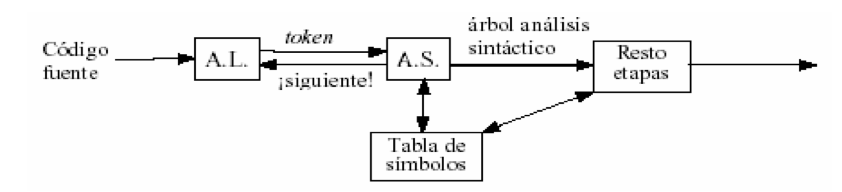
\includegraphics[width=0.8\textwidth]{images/analizadorS}
		\caption{An\'alisis sint\'actico.}
	\end{figure}
	
	\pagebreak
	
	%http://www.udb.edu.sv/udb/archivo/guia/informatica-ingenieria/compiladores/2013/ii/guia-3.pdf
%\section{Gram\'atica simple}

Despu\'es de revisar el an\'alisis del lenguaje natural, el resultado lo podemos expresar mediante un \'arbol. Los \'arboles son formas gr\'aficas que utilizaremos para expresar la estructura de la oraci\'on. \cite{elprofesionaldelainformacion}

	\begin{figure}[htbp!]
		\centering
			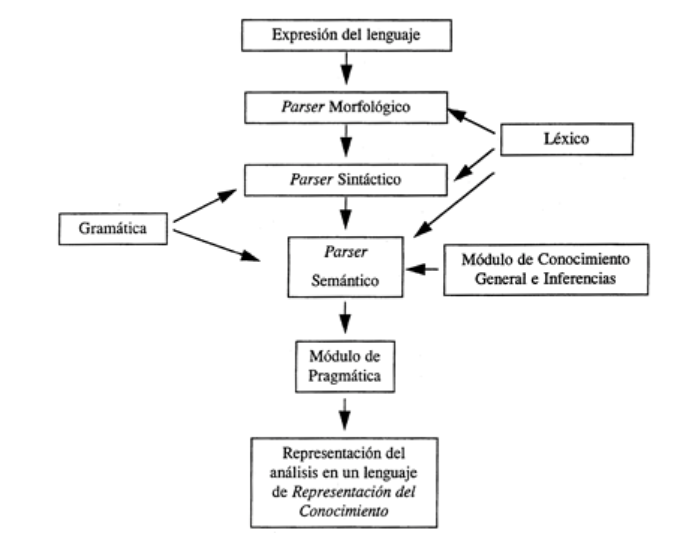
\includegraphics[width=0.8\textwidth]{images/gramatica}
		\caption{Gram\'atica simple}
	\end{figure}
	
%\section{An\'alisis sem\'antico}

En muchas aplicaciones del PLN los objetivos del an\'alisis apuntan hacia el procesamiento del significado. En los \'ultimos a\~nos las t\'ecnicas de procesamiento sint\'actico han experimentado avances significativos, resolviendo los problemas fundamentales.
Sin embargo, las t\'ecnicas de representaci\'on del significado no han obtenido los resultados deseados, y numerosas cuestiones contin\'uan sin encontrar soluciones satisfactorias.
Definir qu\'e es el significado no es una tarea sencilla, y puede dar lugar a diversas interpretaciones. A efectos funcionales, para facilitar el procesamiento, la modularidad es una de las propiedades m\'as deseables. Haciendo uso de esta concepci\'on modular es posible distinguir entre significado independiente y significado dependiente del contexto.
El primero, tratado por la sem\'antica, hace referencia al significado que las palabras tienen por s\'i mismas sin considerar el significado adquirido seg\'un el uso en una determinada circunstancia. La sem\'antica, por tanto, hace referencia a las condiciones de verdad de la frase, ignorando la influencia del contexto o las intenciones del hablante. Por otra parte, el componente significativo de una frase asociado a las circunstancias en que \'esta se da, es estudiado por la pragm\'atica y conocido como significado dependiente del contexto.
Atendiendo al desarrollo en el proceso de interpretaci\'on sem\'antica, es posible optar entre m\'ultiples pautas para su organizaci\'on, tal como se determinan en los siguientes p\'arrafos.
En referencia a la estructura sem\'antica que se va a generar, puede interesarnos que exista una simetr\'ia respecto a la estructura sint\'actica, o por el contrario que no se d\'e tal correspondencia entre ellas. En el primer caso, a partir del \'arbol generado por el an\'alisis sint\'actico se genera una estructura arb\'orea con las mismas caracter\'isticas, sobre la cual se realizar\'a el an\'alisis sem\'antico. En el segundo caso, en la estructura generada por la sintaxis se produce un curso de transformaciones sobre las cuales se genera la representaci\'on sem\'antica.
Cada una de las dos opciones anteriores puede implementarse de forma secuencial o paralela. En la interpretaci\'on secuencial, despu\'es de haber finalizado la fase de an\'alisis sint\'actico, se genera el an\'alisis sem\'antico. En cambio, desde un procedimiento en paralelo, el proceso de an\'alisis sem\'antico no necesita esperar a que el analizador sint\'actico haya acabado toda su tarea, sino que puede ir realizando el an\'alisis de cada constituyente cuando \'este ha sido tratado en el proceso sint\'actico.
Finalmente en combinaci\'on con cada una de las opciones anteriores, podemos escoger un modelo en el que exista una correspondencia entre reglas sint\'acticas y sem\'anticas o, contrariamente, podemos optar por un modelo que no cumpla tal requisito. En caso afirmativo, para cada regla sint\'actica existir\'a una regla sem\'antica correspondiente.
El significado es representado por formalismos conocidos por el nombre de knowledge representation. El l\'exico proporciona el componente sem\'antico de cada palabra en un formalismo concreto, y el analizador sem\'antico lo procesa para obtener una representaci\'on del significado de la frase.

\pagebreak
%\section{An\'alisis pragm\'atico}

A\~nade informaci\'on adicional al an\'alisis del significado de la frase en funci\'on del contexto donde aparece. Se trata de uno de los niveles de an\'alisis m\'as complejos, la finalidad del cual es incorporar al an\'alisis sem\'antico la aportaci\'on significativa que pueden hacer los participantes, la evoluci\'on del discurso o informaci\'on presupuesta.
Incorpora as\'i mismo informaci\'on sobre las relaciones que se dan entre los hechos que forman el contexto y entre diferentes entidades. \cite{elprofesionaldelainformacion}

%\cfinput{MarcoTeorico/reconocimiento}
\section{\textit{Stemming}}
Frecuentemente se usa una palabra para realizar alguna consulta, pero \'unicamente una variable de esa palabra est\'a presente en el texto ya sea en singular, plural, gerundio, etc\'etera.  El problema puede ser resulto con la sustituci\'on de una palabra por todas sus formas.

En la mayor\'ia de los casos, las variantes morfol\'ogicas de las palabras tienen interpretaciones sem\'anticas similares y se pueden considerar como equivalentes. Por esta raz\'on, se han desarrollado algoritmos de derivaci\'on, o analizadores ling\"u\'isticos, que tratan de reducir una palabra a su \textit{stem} o ra\'iz. Por lo tanto, los t\'erminos clave de una consulta o documento est\'an representados por las ra\'ices en lugar de las palabras originales. Esto no s\'olo significa que las diferentes variantes de un t\'ermino pueden confundir a una sola forma representativa, sino que tambi\'en reduce el tama\~no del diccionario, es decir, el n\'umero de t\'erminos distintos necesario para la representaci\'on de un conjunto de documentos. A peque\~nos resultados del tama\~no del diccionario en un ahorro de espacio de almacenamiento y tiempo de procesamiento.

El \textit{Stemming} es un m\'etodo utilizado para reducir una palabra a su ra\'iz. \cite{stemm}

\pagebreak
\section{Lematizaci\'on}
Uno de los procesos fundamentales para tratar los textos ling\"u\'isticos es la lematizaci\'on, que consiste en asignar una forma representativa a distintas formas concretas variables: formas conjugadas del verbo, cambios seg\'un el g\'enero y n\'umero de adjetivos y sustantivos, etc. Es necesario a la hora de realizar unos estudios estad\'isticos, redactar un vocabulario o diccionario, intentar una b\'usqueda de informaci\'on por palabras clave y analizar la combinaci\'on de elementos, entre otros objetivos de investigaci\'on.

Este proceso puede involucrar tareas complejas como entender el contexto de una categor\'ia gramatical de una palabra dentro de una oraci\'on. 

En muchos idiomas, las palabras aparecen flexionadas de difentes maneras. Por ejemplo en espa\~nol el verbo 'caminar' puede aparecer como 'camino', 'camin\'o', 'camin\'a' 'caminando'. La forma base 'caminar', que puede ser buscada y encontrada en un diccionario, es llamada lema de la palabra. La combinaci\'on de la foma base con la flexi\'on es llamada lexema de la palabra.


La importancia de la lematizaci\'on radica en el hecho que, para acceso por contenido a bases de datos textuales, permite superar las limitaciones de una b\'usqueda simple de strings, haciendo que relaciones ocultas por la variabilidad morfol\'ogica de las palabras queden manifiestas. La lematizaci\'on mejora por lo tanto el recubrimiento (recall) aunque pueda ser a expensas de la precisi\'on cuando diferentes conjugaciones morfol\'ogicas de una misma raiz est\'an asociadas a conceptos distintos.

La lematizaci\'on est\'a muy relacionada con el etiquetado autom\'atico de textos (POS tagging), que consiste en atribuir a cada palabra su categor\'ia gramatical, ya que la categor\'ia puede determinarse por las flexiones o derivaciones (ej: en castellano -ar indica un infinitivo, -ado un participio pasado masculino singular, etc.). Muchos esquemas de procesamiento de textos, aplicados a lenguas flexivas europeas, plantean un etiquetado autom\'atico previo a la lematizaci\'on, de manera que al lematizar se cuente con la informaci\'on de la categor\'ia gramatical de las palabras. Sin embargo, la atribuci\'on de etiquetas correctas depende en general de una lematizaci\'on impl\'icita basada en un an\'alisis de sufijos y prefijos, lo que permite una primera predicci\'on que se corrige, en una segunda etapa, en funci\'on del contexto immediato de la palabra analizada (Brill). Esta manera de proceder presenta algunos problemas: (i) requiere de un corpus manualmente etiquetado de gran dimensi\'on para derivar reglas de etiquetado autom\'atico adecuadas, (ii) no aprovecha la existencia de paradigmas de conjugaci\'on o derivaci\'on, (iii) s\'olo considera ra\'ices libres. \cite{lem}

\section{\textit{Stopwords}}
Las palabras que aparecen con frecuencia entre los documentos no son buenas para la recuperaci\'on de informaci\'on. As\'i palabras que aparecen en m\'as del 80 porciento de documentos no son consideradas y se les llama \textit{stopwords} \cite{sw} : 
 \begin{itemize}
 \item Los art\'iculos, los pronombres, las preposiciones, y las conjunciones son candidatos naturales. 
 \item Algunos verbos, adverbios, y adjetivos se pod\'ian tratar como \textit{stopwords}. 
 \item Los t\'erminos espec\'ificos de un dominio se pod\'ian tratar como \textit{stopwords}.
Se suele tener una lista de palabras que no son buenos t\'erminos de indexaci\'on llamada STOPLIST, Lista de Palabras Vac\'ias o Diccionario Negativo. La salida del analizador l\'exico es comprobada con la STOPLIST y se eliminan los t\'erminos que aparecen en ella. Tambi\'en se puede realizar la comprobaci\'on durante la etapa del an\'alisis l\'exico (esto para mejorar el rendimiento) pero no suele ser muy usado en muchos casos.
\end{itemize}

Ventajas: 
 \begin{itemize}
 \item Las palabras vac\'ias aparecen mucho y su lista de referencias es muy grande: 
 \item Si las quitamos el archivo invertido ser\'a m\'as peque\~no. 
 \item El archivo invertido se reduce en un 30 \'o 40 porciento. 
 \item Mejora la eficiencia, porque hay una mejor selecci\'on de palabras claves. 
 \item La indexaci\'on es m\'as r\'apida.
 \end{itemize}
Desventajas: 
 \begin{itemize}
 \item Por otro lado, la eliminaci\'on de \textit{stopwords} puede reducir el recall, lo que hace que sea interesante la indexaci\'on del texto completo.
 \end{itemize}
%\section{Online Grooming}
El online Grooming es un fenómeno que podr\'iamos traducir como engatusamiento y que se utiliza para describir las pr\'acticas online de ciertos adultos para ganarse la confianza de un (o una) menor fingiendo empat\'ia, cariño, etc. con fines de satisfacción sexual (como m\'inimo, y casi siempre, obtener im\'agenes del menor desnudo o realizando actos sexuales).

Por tanto est\'a muy relacionado con la pederastia y la pornograf\'ia infantil en Internet. De hecho el grooming es en muchas ocasiones la antesala de un abuso sexual \cite{grooming}.

\subsection{Caracterización del online grooming}
De acuerdo al art\'iculo ``Characterizing pedophile conversations on the Internet using Online Grooming Web.'' \cite{articulo} son 6 las etapas por las cuales una conversaci\'on con corpotanemiento peligroso suele pasar. 
La tabla \ref{table:caracterizacion} muestra la descripci\'on por los cuales una conversaci\'on tiende a incidir en el caso de conversaciones peligrosas.

\begin{table}[h]

\begin{tabular}[t]{|p{15mm} |p{22mm} |p{22mm} |p{22mm} |p{20mm} |p{20mm} |p{20mm} |}
\hline
\hline
Etapas & Formaci\'on de la amistad & Formaci\'on de una relaci\'on & Evaluaci\'on de riesgos & Exclusividad & Sexual & Conclusi\'on \\
\hline
Descriptor1 & Intercambio de cuentas de correo electr\'onico, fotograf\'ias, webcam, informaci\'on & Intercambio de cuentas de correo electr\'onico, fotograf\'ias, webcam, informaci\'on & Evaluar a los padres del ni\~no, si est\'an alrededor o qui\'en puede ver su computadora & Sentir amor y expresar exclusividad & Dar descripci\'on del cuerpo y la figura & Quedar un d\'ia, una cita, hora, lugar para conocerse en persona \\
\hline
Descriptor2 &Hablar de novios/novias & Dar suaves cumplidos & Pedir al ni\~no eliminar su historial de conversaciones, asegurarse quenadie tenga la contrase\~na & Describir actividad sexual y experiencias al ni\~no &Ser novios &Discutir puntos en com\'un para una reuni\'on \\
\hline
Descriptor3 &Obtener informaci\'on del perfil y otras cuentas del ni\~no & hablar de los hobbies del a\~no, actividades e intereses & Ver si el ni\~no est\'a c\'omodo con ver a alguien mayor& Cumplidos fuertes & Intercambiar fotograf\'ias sexuales & Asegurarse de que el ni\~no ir\'a s\'olo \\
\hline
Descriptor4 & Preguntar la edad, genero, localidad, nombre, informaci\'on personal, detalles familiares & Escuela, grado, tareas, n\'umero de celular & Asegurarse de que el ni\~no no es un polic\'ia & Construir confianza entre el ni\~no y el ped\'ofilo & Dar orientaci\'on sexual, cumplidos & Decidir qu\'e hacer cuando se conozcan\\
\hline
\end{tabular} \\ \\ \\
\caption{Tabla de caracterizaci\'on del comportamiento de conversaciones peligrosas}
\label{table:caracterizacion}
\end{table}


%=========================================================

\chapter{Especificaciones del proyecto}
%---------------------------------------------------------
\section{Objetivo}
%---------------------------------------------------------
\subsection{Objetivo general}
Desarrollar un sistema que sea capaz de analizar y clasificar texto en diferentes categor\'ias a partir de un conjunto de datos estad\'isticos mediante: reconocimiento de patrones, aprendizaje m\'aquina y miner\'ia de datos. A fin de poder clasificar conversaciones como peligrosas o no peligrosas.\\ 



%---------------------------------------------------------
\subsection{Objetivos espec\'ificos}
Desarrollar: \\ 

	\begin{itemize}
	\item Aplicaci\'on para el intercambio de conversaciones.
	\item API  para el an\'alisis de conversaciones.
	\item Aplicaci\'on para el procesamiento de texto.
	\item Aplicaci\'on que funcione, como conexi\'on entre los m\'odulos del sistema.
	\item Un set de pruebas de desempe\~no del sistema para verificar su eficiencia.
	\end{itemize}

\section{Metodología}

Se consideró utilizar el modelo de desarrollo evolutivo o prototipo evolutivo ya que construye una serie de grandes versiones
sucesivas de un producto. Sin embargo, mientras que la aproximación incremental presupone que el conjunto completo de
requerimientos es conocido al comenzar, el modelo evolutivo. En este modelo, los requerimientos son cuidadosamente
examinados, y sólo esos que son bien comprendidos son seleccionados para el primer incremento. Los desarrolladores construyen
una implementación parcial del sistema que recibe sólo estos requerimientos.
Aplicaremos la metodología de la siguiente forma:\\

\begin{itemize}
	\item Planificación: especificaremos los requerimientos que se necesitan en cada uno de los módulos para su correcto
funcionamiento.

	\item Desarrollo: se realizará el módulo y las pruebas de funcionamiento antes de proseguir para la retroalimentación del cliente.
	
	\item Retroalimentación de parte del cliente: las pruebas serán realizadas por el cliente para poder tener la retroalimentación y
así exponer al sistema a una prueba en el entorno que será utilizado finalmente.
	
	\item Modificaciones: si se requieren se realizaran mejoras de acuerdo a los resultados obtenidos por el cliente, de no tener
alguna modificación se pasara a la siguiente fase hasta terminar el sistema.\\

\end{itemize}


\begin{figure}
	\centering
	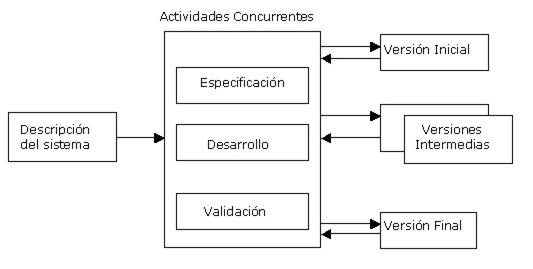
\includegraphics[scale=.7]{images/metodologia}
	\caption{Ciclo de vida de la metodología de prototipos.}
	\label{fig:metodologia}
\end{figure}


Los módulos del proyecto así como la documentación serán realizados en el siguiente orden:

\begin{itemize}
	\item Sensor y analizador
	
	\item Motor de interferencia
	
	\item Acciones de respuesta
	
	\item Registrador de eventos\\
\end{itemize}
\section{Descripción}

Una vez definidos lo que son los IDS procederemos a los requisitos funcionales de cada componente del proyecto. \\

\subsection{Descripción Sensor IDS}

Requisitos funcionales \\

\begin{itemize}
    \item Se debe poder especificar los puertos de lectura de paquetes en el servidor.
    \item Los parametros de configuración del sensor deben estar ubicados en un archivo de configuración .conf
    \item Solo se interceptaran y monitorearán paquetes HTTP/HTTPS.
    \item Para el caso del protocólo HTTPS el sistema deberá poder decodificiar el paquete usando las llaves generadas por el servidor.
    \item Implementar un algoritmo de \textit{machine learning} para identificar y asignar un rating de peligrosidad.
    \item Generar archivos logs con la fecha del evento, conexión o ID de sesión, conexión TCP, tipo de alerta, rating, protocolo, IP fuente y destino, puertos fuente y destino, cantidad de bytes transferidos, información del paquete decodificada.
    \item Utilizar concurrencia para ir liberando la carga de lectura de paquetes y aumentar la velocidad del sensor.
\end{itemize}

Requisitos no funcionales \\

% \begin{itemize}
%     \item Se debe poder especificar los puertos de lectura de paquetes en el servidor.
% \end{itemize}

\subsection{Descripción registrador de eventos}

Requisitos funcionales \\

\begin{itemize}
    \item Se debe poder especificar la ruta donde se generarán los logs que vienen desde el IDS del sensor.
    \item Se debe poder especificar la conexión a base de datos en la que se guardarán los eventos obtenidos de los logs.
    \item Se debe poder especificar la conexión a un servicio de caché que permita conectarse a un servidor de websockets para enviar notificaciones.
    \item Se debe poder especificar la conexión a un servicio de mail que permita enviar correos a los administradores del IDS.
    \item Los parametros de configuración del registrador de eventos tales como conexión a base de datos, url de los logs, etc. deben estar ubicados en un archivo de configuración .conf
    \item Leer archivos logs que provengan del IDS sensor
    \item Analizar estructura de logs coincida con la estructura de un evento
    \item Guardar eventos obtenidos desde los logs en una base de datos local o remota.
    \item Guardar eventos obtenidos desde los logs en una servicio de caché local o remoto.
    \item Enviar mail de acuerdo a las configuraciones por administrador de la consola para cada evento.
    \item El envío de mails debe de implementar concurrencia para evitar la carga de recursos al sistema.
\end{itemize}

Requisitos no funcionales \\

% \begin{itemize}
%
% \end{itemize}

\subsection{Descripción consola de administración}

Requisitos funcionales \\

\begin{itemize}
    \item Se deberán poder administrar usuarios para el sistema.
    \item Los usuarios del sistema pueden iniciar sesión.
    \item La contraseña de los usuarios tiene que estar encriptada con un algoritmo sha256.
    \item Deberán existir permisos para la realización de actividades dentro del sistema.
    \item Deberá existir siempre forzozamente un usuario de tipo superuser encargado de administrar todo el sistema, es decir contará con todos los permisos del sistema.
    \item Puede existir más de un superuser.
    \item Los usuarios superusers, podrán dar de alta otros usuarios superusers.
    \item Existe de la posibilidad de que haya usuarios tipo administrador con permisos especificos dentro del sistema.
    \item Los usuarios superusers, podrán dar de alta, modificar y eliminar a los usuarios adiministradores y administrar sus permisos.
    \item Los usuarios no se eliminan en su totalidad, solo se desactivan y se almacena la fecha que se desactivó.
    \item Los usuarios superusers, podrán eliminar otros usuarios superuser pero no a él mismo.
    \item Los usuarios podrán cambiar su contraseña en cualquier momento.
    \item Deberán existir grupos para así asignar permisos a un grupo y relacionar los usuarios con ese grupo.
    \item Deberán poderse administrar los permisos de los grupos.
    \item El sistema debe ser capaz de conectarse a la base de datos del IDS para obtener los eventos registrados.
    \item Deberá existir un permiso para ver los eventos del sistema.
    \item No se pueden eliminar eventos de la base de datos del IDS
    \item Se puede cambiar el estatus de los eventos en la base de datos del IDS y asignar una acción preventiva al evento.
    \item Todas las acciones de los usuarios se deben almacenar con la fecha, la acción y un mensaje del porqué se realizó ese cambio.
    \item Deberá existir un permiso para recibir notificaciones.
    \item Los usuarios superuser siempre tendrán permisos para recibir notificaciones.
    \item Si se tiene permiso para recibir notificaciones se deben poder administrar estás notificaciones según el tipo.
    \item Deberá existir un permiso para generar reportes.
    \item Los usuarios superuser siempre tendrán permisos para generar reportes.
    \item Los reportes se deben poder descargar en formato PDF.
    \item Deberá exsitir una vista con el índice de todos los eventos generados por el IDS y se deberá poder filtrar por ranking, status, protocólo y fecha.
    \item Es necesario que exista un monitoreo de eventos en tiempo real.
\end{itemize}

Requisitos no funcionales \\

% \begin{itemize}
%
% \end{itemize}

\section{Arquitectura del sistema}

El sistema contendr\'a los siguientes modulos:
\begin{description}
\item[Sistema de Mensajer\'ia] Este modulo del sistema ser\'a el encargado de generar informaci\'on de pruebas para posteriormente ser procesada.

\item[Procesamiento de texto] Este m\'odulo tiene como objetivo el recibir un archivo de texto con la conversaci\'on a analizar el cual fue generado en el m\'odulo de mensajer\'ia. La salida de \'este ser\'a una estructura invariante para poder ser analizada.

\item[API de an\'alisis] Ser\'a el módulo que mediante reconocimiento de patrones, har\'a una revisión de los textos para poder clasificar a una fuente en un comportamiento.

\item[M\'odulo integrador]Este m\'odulo es el encargado de presentar de forma visual los resultados obtenidos del proceso de clasificación de conversaciones. 

\item[Base de conocimiento] Contendr\'a  un conjunto de datos referentes al caso de estudio, que son necesarios para la clasificación de las fuentes. 

\end{description}


La figura \ref{arquitectura} muestra la arquitectura general del sistema de an\'alisis de texto.
\begin{figure}[h]
\begin{center}

    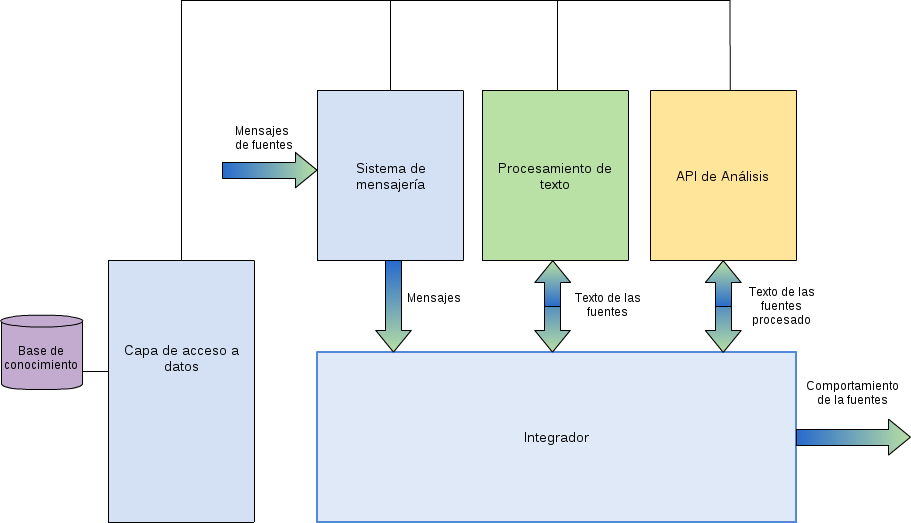
\includegraphics[scale=.5]{images/arquitectura}
  \caption{Arquitectura general del sistema}
  \label{arquitectura}
  \end{center}
\end{figure}

%\appendix
%=========================================================
%\chapter{Prototipo 1: Almacenamiento de fuentes}
%\section{Marco Te\'orico}
Tomando en consideraci\'on la matriz de caracterizaci\'on del prototipo anterior. Este prototipo toma como base el Nivel 5 para la extracci\'on de caracter\'isticas pertenecientes a este nivel.

Retomando la tabla \ref{table:caracterizacion} del prototipo anterior, el Nivel 5 contiene una serie de de descriptores de car\'acter sexual. En este nivel el tipo de vocabulario que contienen las conversaciones es meramente relacionado con el contexto sexual.

A diferencia del nivel anterior en este prototipo se trabajar\'a \'unicamente con palabras en lugar de frases, debido a que con base en la observaci\'on el contexto bajo el cual las palabras aparecen es meramente sexual. Decidimos \'unicamente trabajar con la siguiente lista de palabras y sus respectivas derivaciones:

\begin{itemize}
\item Chupar. 
\item Coger. 
\item Follar. 
\item Lamer. 
\item Besar. 
\item Pene. 
\item Vagina. 
\item Masturbar. 
\item Sexo. 
\item Pechos. 
\item Tetas.
\item Clitoris.
\item Tragar.
\end{itemize}


Haciendo una estad\'istica de la frecuencia del stemm de palabras con denotac\'on sexual, se obtuvieron las siguientes gr\'aficas mostradas en las figuras \ref{fig:graficasexual1} y \ref{fig:graficasexual2}. Se puede apreciar que la diferencia de frecuencia de aparici\'on de palabras est\'a muy marcada. Pues en conversaciones no peligrosas la frecuencia es en la mayor\'ia de los casos 0, mientras que en las peligrosas est\'a muy marcada la frecuencia de estas pablabras.

\begin{figure}[h]
\begin{center}
	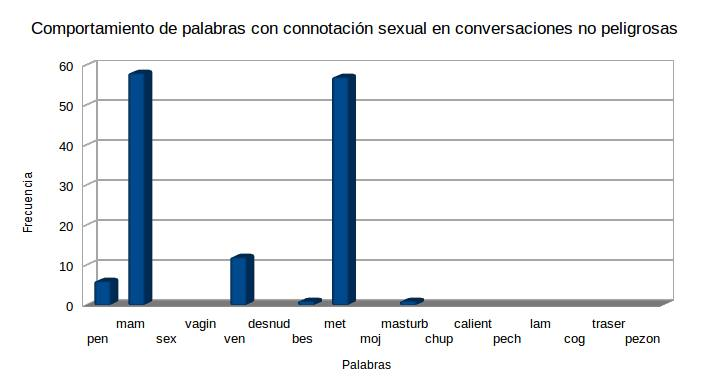
\includegraphics[scale=.6]{images/palabrassexuales1}
	\caption{Frecuencia de palabras de car\'acter sexual en conversaciones no peligrosas}
	\label{fig:graficasexual1}
\end{center}
\end{figure}


\begin{figure}[h]
\begin{center}
	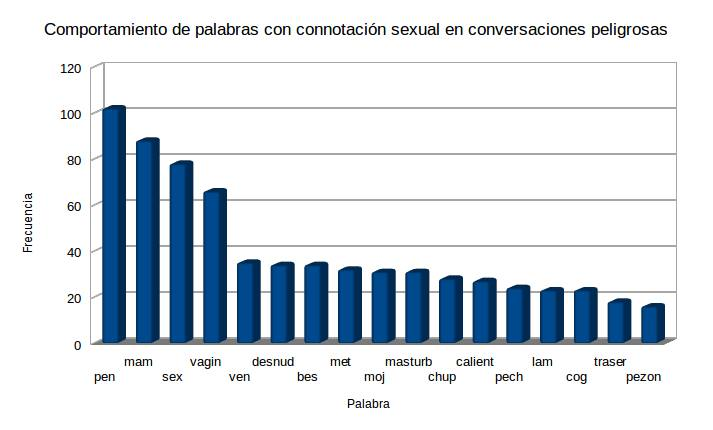
\includegraphics[scale=.6]{images/palabrassexuales2}
	\caption{Frecuencia de palabras de car\'acter sexual en conversaciones peligrosas}
	\label{fig:graficasexual2}
\end{center}
\end{figure}

\section{Descripci\'on}

Este prototipo genera vectores de frecuencia de las palabras del Nivel 5 de la matriz de caracterizaci\'on del comportamiento de conversaciones enfocadas al Online grooming.
\section{Objetivo}
Crear un prototipo que genere vectores de frecuencia de acuerdo al diccionario de palabras correspondientes al Nivel 5 de la matriz de frecuencias de la caracterizaci\'on del comportamiento de conversaciones enfocadas al Online grooming..

\section{An\'alisis}
\subsection{Caracter\'isticas}

\begin{description}
\item[FEAT1] El sistema recibe como entrada una conversaci\'on almacenada en un archivo de texto plano.
\item[FEAT2] El sistema recibe como entrada un archivo una conversaci\'on con un formato xml.
\item[FEAT2] Las palabras del diccionario son editables.
\item[FEAT3] El sistema genera el vector de frecuencias de acuerdo al diccionario dado.
\end{description}

\subsection{Restricciones}
\begin{itemize}
\item Persistencia de vectores en archivos.
\item Lenguaje de programaci\'on python.
\end{itemize}


\section{Dise\~no}

La figura \ref{fig:arquitectura_vector} muestra la arquitectura del comportamiento del prototipo, la cual recibe como entrada las conversaciones en formato plano o con formato xml y como salida se obtiene un vector asociado el cual representa la frecuencia de palabras que pertenecen al Nivel 5 de la matriz de caracterizaci\'on.

\begin{center}
	\begin{figure}[h]
		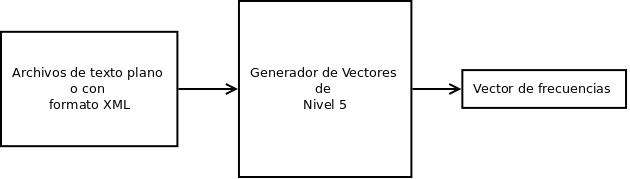
\includegraphics[scale=.5]{images/diagramavectores}
		\caption{Arquitectura Protipo 2}
		\label{fig:arquitectura_vector}
	\end{figure}
\end{center}


En la figura \ref{fig:diagramaActividades} se muestra el diagrama de actividades de la generac\'on de vectores del prototipo. En primer lugar se obtienen las conversaciones de las cuales queremos calcular el vector. El siguiente paso es ignorar palabras sin significado las cuales denominamos stopwords. Obtenemos la ra\'iz mediante el algoritmo de stemming de las palabras. Comparamos las palabras con el diccionario de palabras que tenemos del nivel 5, es decir, las palabras anteriormente listadas. Si la ra\'iz de la palabra que estamos analizando coincide con alguna de nuestro diccionario entonces aumentamos en 1 el valor de la componente del vector que est\'a asociada a dicha palabra.

	\begin{figure}[h]
	\begin{center}
		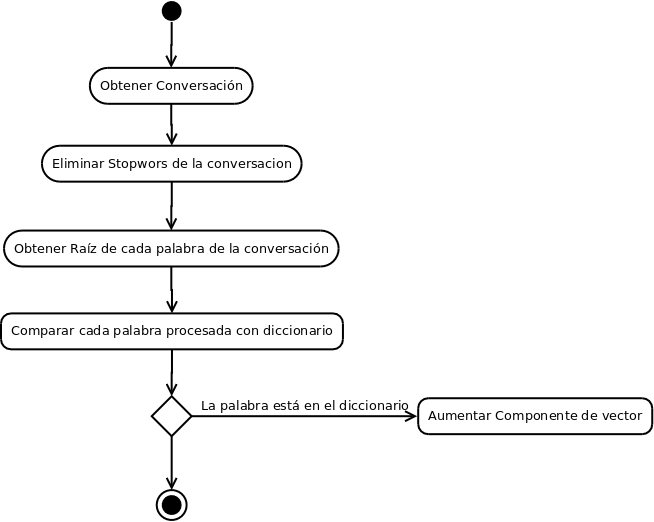
\includegraphics[scale=.35]{images/actividades_vectores}
		\label{fig:diagramaActividades}
		\caption{Diagrama de Actividades del Generador de Vectores}
		\end{center}
	\end{figure}


\section{Resultados}
\subsection{Pruebas}
El prototipo se probó con la generaci\'on de vectores de dimenciones de 3 componentes y 13 componentes.

Las componentes del primer tipo de vector est\'an asociadas al siguiente conjunto de palabras:
\begin{itemize}
\item Lista 1: desnudo, pene, vagina. 

Las componentes del segundo tipo de vector est\'an asociadas al siguiente conjunto de palabras:

\item Lista 2: chupar, coger, follar, lamer, besar, pene, vagina, masturbar, sexo, pechos, tetas, clitoris, tragar.
\end{itemize}

Para ambas listas de palabras se generaron los vectores correspondientes a 50 conversaciones extra\'idas del portal \url{http://www.perverted-justice.com/}, el cual, como ya se hab\'ia mencionado antes, es un sitio donde se hacen p\'ublicas conversaciones que han servido de anzuelo para capturar ped\'ofilos en internet. Estas conversaciones fueron traducidas al español y se anexan en el ap\'endice \ref{app:conversaciones}.


De igual manera se obtuvieron las caracter\'isticas de 50 conversaciones no peligrosas extra\'idas de conversaciones diarias de nuestras cuentas personales de Facebook anexadas en el aprendice \ref{app:conversacionesnp}.

La figura \ref{fig:graficaVectores} muestra la gr\'afica que contiene los vectores de 3 componentes generados por el prototipo. Marcados con puntos amarillos los vectores que representan la clase peligrosa, como podemos observar est\'an en el centro del plano. Mientras que las no peligrosas tienen una disperci\'on fuera del centro. 

Con esto podemos formular una hip\'otesis donde las conversaciones no peligrosas se posicionan en el origen del plano. Con esto podemos decir que este problema es linealmente separable cosa que nos ayudar\'a en la construcci\'on del clasificador. 

\begin{center}
\begin{figure}[h]
	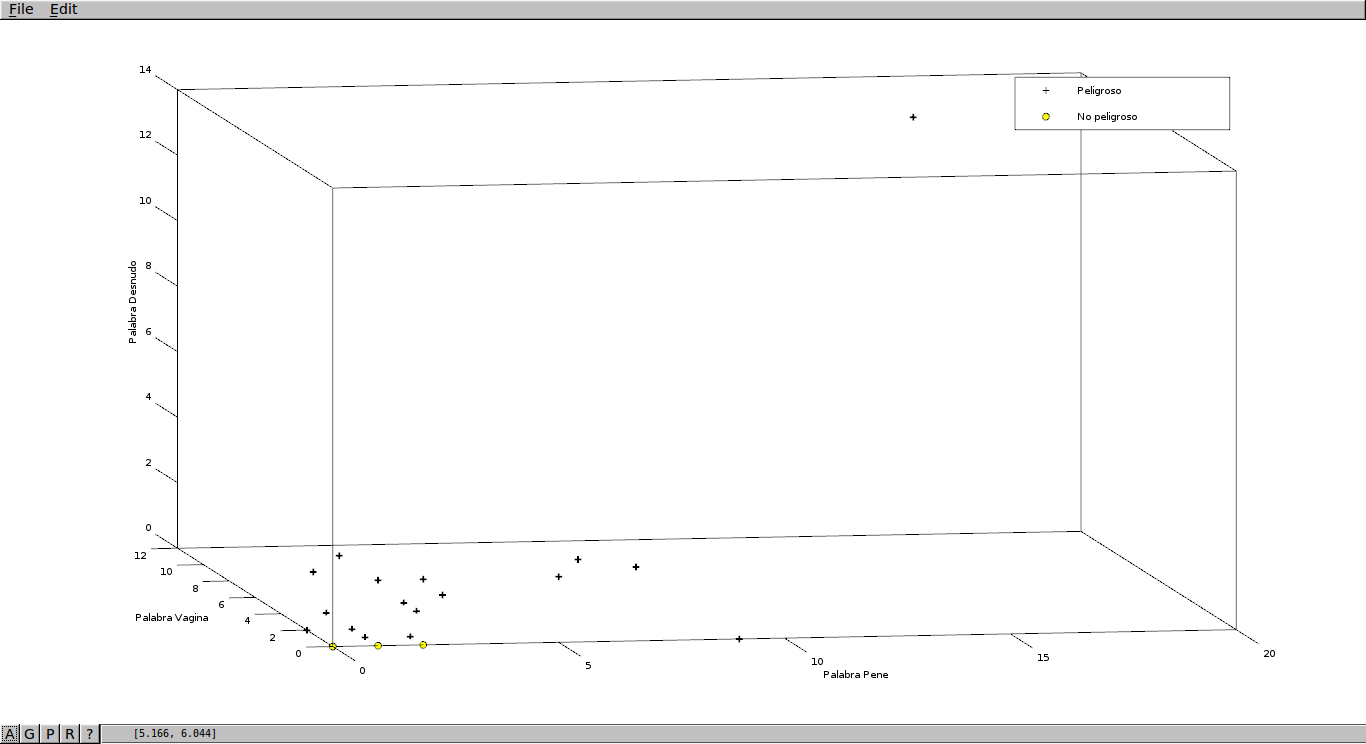
\includegraphics[scale=.3]{images/vectores}
	\caption{Gr\'afica de vectores generados}
	\label{fig:graficaVectores}
\end{figure}
\end{center}

Al aumentar el n\'umero de caracter\'iscas, esperamos que la separabilidad de las clases sea a\'un m\'as evidente por eso hemos seleccionado 13 caracter\'isticas para entrenar al clasificador del prototipo 3.
	
%% \IUref{IUAdmPS}{Administrar Planta de Selección}
% \IUref{IUModPS}{Modificar Planta de Selección}
% \IUref{IUEliPS}{Eliminar Planta de Selección}

% 


% Copie este bloque por cada caso de uso:
%-------------------------------------- COMIENZA descripción del caso de uso.

%\begin{UseCase}[archivo de imágen]{UCX}{Nombre del Caso de uso}{
	\begin{UseCase}{CU3}{Enviar mensaje}{El caso de uso permite al Contacto enviar mensajes de texto a trav\'es de un canal abierto de comunicaci\'on.
	}
		\UCitem{Versi\'on}{0.2}
		\UCitem{Actor}{Contacto}
		\UCitem{Prop\'osito}{Enviar y Almacenar los mensajes escritos enviados entre los usuarios del sistema de mensajer\'ia, para su an\'alisis en el desarrollo de los m\'odulos posteriores.}
		\UCitem{Resumen}{
		El caso de uso permite al usuario enviar mensajes atrav\'es del un canal de comunicacion abierto}
		\UCitem{Entradas}{Mensaje string  (obligatorio)}
		\UCitem{Salidas}{Historial de mensajes enviados y recibidos }
		\UCitem{Precondiciones}{El usuario debera tener un canal de comunicaci\'on abierto.El mensaje no puede estar vac\'io.}
		\UCitem{Postcondiciones}{Los mensajes enviados y recibidos podr\'an ser visualidaos por ambos usuarios que comparten el mismo canal}		
		\UCitem{Autor}{Anah\'i Ruiz D\'iaz}
	\end{UseCase}

	\begin{UCtrayectoria}{Principal}
	
		\UCpaso[\UCactor] El usuario escribe un mensaje dentro de una caja de textos.
		\UCpaso[\UCactor] El usuario da clic en el bot\'on \IUbutton{Enviar} para enviar el mensaje. 

		\UCpaso  El sistema env\'ia y muestra al otro Contacto el mensaje enviado por el usuario.  \Trayref{A}.
		\UCpaso[] Fin del flujo.
				
	\end{UCtrayectoria}
		
		\begin{UCtrayectoriaA}{A}{Mensaje no enviado}
			\UCpaso El sistema muestra una alerta que notifica al usuario que ocurri\'o un error y su mensaje no fue enviado.
			\UCpaso[] El usuario da clic en el bot\'on \IUbutton{Aceptar}.
			\UCpaso[] Fin del flujo.
		\end{UCtrayectoriaA}


%-------------------------------------- TERMINA descripción del caso de uso.
%% \IUref{IUAdmPS}{Administrar Planta de Selección}
% \IUref{IUModPS}{Modificar Planta de Selección}
% \IUref{IUEliPS}{Eliminar Planta de Selección}

% 


% Copie este bloque por cada caso de uso:
%-------------------------------------- COMIENZA descripción del caso de uso.

%\begin{UseCase}[archivo de imágen]{UCX}{Nombre del Caso de uso}{
	\begin{UseCase}{CU3}{Enviar mensaje}{El caso de uso permite al Contacto enviar mensajes de texto a trav\'es de un canal abierto de comunicaci\'on.
	}
		\UCitem{Versi\'on}{0.2}
		\UCitem{Actor}{Contacto}
		\UCitem{Prop\'osito}{Enviar y Almacenar los mensajes escritos enviados entre los usuarios del sistema de mensajer\'ia, para su an\'alisis en el desarrollo de los m\'odulos posteriores.}
		\UCitem{Resumen}{
		El caso de uso permite al usuario enviar mensajes atrav\'es del un canal de comunicacion abierto}
		\UCitem{Entradas}{Mensaje string  (obligatorio)}
		\UCitem{Salidas}{Historial de mensajes enviados y recibidos }
		\UCitem{Precondiciones}{El usuario debera tener un canal de comunicaci\'on abierto.El mensaje no puede estar vac\'io.}
		\UCitem{Postcondiciones}{Los mensajes enviados y recibidos podr\'an ser visualidaos por ambos usuarios que comparten el mismo canal}		
		\UCitem{Autor}{Anah\'i Ruiz D\'iaz}
	\end{UseCase}

	\begin{UCtrayectoria}{Principal}
	
		\UCpaso[\UCactor] El usuario escribe un mensaje dentro de una caja de textos.
		\UCpaso[\UCactor] El usuario da clic en el bot\'on \IUbutton{Enviar} para enviar el mensaje. 

		\UCpaso  El sistema env\'ia y muestra al otro Contacto el mensaje enviado por el usuario.  \Trayref{A}.
		\UCpaso[] Fin del flujo.
				
	\end{UCtrayectoria}
		
		\begin{UCtrayectoriaA}{A}{Mensaje no enviado}
			\UCpaso El sistema muestra una alerta que notifica al usuario que ocurri\'o un error y su mensaje no fue enviado.
			\UCpaso[] El usuario da clic en el bot\'on \IUbutton{Aceptar}.
			\UCpaso[] Fin del flujo.
		\end{UCtrayectoriaA}


%-------------------------------------- TERMINA descripción del caso de uso.
%% \IUref{IUAdmPS}{Administrar Planta de Selección}
% \IUref{IUModPS}{Modificar Planta de Selección}
% \IUref{IUEliPS}{Eliminar Planta de Selección}

% 


% Copie este bloque por cada caso de uso:
%-------------------------------------- COMIENZA descripción del caso de uso.

%\begin{UseCase}[archivo de imágen]{UCX}{Nombre del Caso de uso}{
	\begin{UseCase}{CU3}{Enviar mensaje}{El caso de uso permite al Contacto enviar mensajes de texto a trav\'es de un canal abierto de comunicaci\'on.
	}
		\UCitem{Versi\'on}{0.2}
		\UCitem{Actor}{Contacto}
		\UCitem{Prop\'osito}{Enviar y Almacenar los mensajes escritos enviados entre los usuarios del sistema de mensajer\'ia, para su an\'alisis en el desarrollo de los m\'odulos posteriores.}
		\UCitem{Resumen}{
		El caso de uso permite al usuario enviar mensajes atrav\'es del un canal de comunicacion abierto}
		\UCitem{Entradas}{Mensaje string  (obligatorio)}
		\UCitem{Salidas}{Historial de mensajes enviados y recibidos }
		\UCitem{Precondiciones}{El usuario debera tener un canal de comunicaci\'on abierto.El mensaje no puede estar vac\'io.}
		\UCitem{Postcondiciones}{Los mensajes enviados y recibidos podr\'an ser visualidaos por ambos usuarios que comparten el mismo canal}		
		\UCitem{Autor}{Anah\'i Ruiz D\'iaz}
	\end{UseCase}

	\begin{UCtrayectoria}{Principal}
	
		\UCpaso[\UCactor] El usuario escribe un mensaje dentro de una caja de textos.
		\UCpaso[\UCactor] El usuario da clic en el bot\'on \IUbutton{Enviar} para enviar el mensaje. 

		\UCpaso  El sistema env\'ia y muestra al otro Contacto el mensaje enviado por el usuario.  \Trayref{A}.
		\UCpaso[] Fin del flujo.
				
	\end{UCtrayectoria}
		
		\begin{UCtrayectoriaA}{A}{Mensaje no enviado}
			\UCpaso El sistema muestra una alerta que notifica al usuario que ocurri\'o un error y su mensaje no fue enviado.
			\UCpaso[] El usuario da clic en el bot\'on \IUbutton{Aceptar}.
			\UCpaso[] Fin del flujo.
		\end{UCtrayectoriaA}


%-------------------------------------- TERMINA descripción del caso de uso.
%% \IUref{IUAdmPS}{Administrar Planta de Selección}
% \IUref{IUModPS}{Modificar Planta de Selección}
% \IUref{IUEliPS}{Eliminar Planta de Selección}

% 


% Copie este bloque por cada caso de uso:
%-------------------------------------- COMIENZA descripción del caso de uso.

%\begin{UseCase}[archivo de imágen]{UCX}{Nombre del Caso de uso}{
	\begin{UseCase}{CU3}{Enviar mensaje}{El caso de uso permite al Contacto enviar mensajes de texto a trav\'es de un canal abierto de comunicaci\'on.
	}
		\UCitem{Versi\'on}{0.2}
		\UCitem{Actor}{Contacto}
		\UCitem{Prop\'osito}{Enviar y Almacenar los mensajes escritos enviados entre los usuarios del sistema de mensajer\'ia, para su an\'alisis en el desarrollo de los m\'odulos posteriores.}
		\UCitem{Resumen}{
		El caso de uso permite al usuario enviar mensajes atrav\'es del un canal de comunicacion abierto}
		\UCitem{Entradas}{Mensaje string  (obligatorio)}
		\UCitem{Salidas}{Historial de mensajes enviados y recibidos }
		\UCitem{Precondiciones}{El usuario debera tener un canal de comunicaci\'on abierto.El mensaje no puede estar vac\'io.}
		\UCitem{Postcondiciones}{Los mensajes enviados y recibidos podr\'an ser visualidaos por ambos usuarios que comparten el mismo canal}		
		\UCitem{Autor}{Anah\'i Ruiz D\'iaz}
	\end{UseCase}

	\begin{UCtrayectoria}{Principal}
	
		\UCpaso[\UCactor] El usuario escribe un mensaje dentro de una caja de textos.
		\UCpaso[\UCactor] El usuario da clic en el bot\'on \IUbutton{Enviar} para enviar el mensaje. 

		\UCpaso  El sistema env\'ia y muestra al otro Contacto el mensaje enviado por el usuario.  \Trayref{A}.
		\UCpaso[] Fin del flujo.
				
	\end{UCtrayectoria}
		
		\begin{UCtrayectoriaA}{A}{Mensaje no enviado}
			\UCpaso El sistema muestra una alerta que notifica al usuario que ocurri\'o un error y su mensaje no fue enviado.
			\UCpaso[] El usuario da clic en el bot\'on \IUbutton{Aceptar}.
			\UCpaso[] Fin del flujo.
		\end{UCtrayectoriaA}


%-------------------------------------- TERMINA descripción del caso de uso.
%% \IUref{IUAdmPS}{Administrar Planta de Selección}
% \IUref{IUModPS}{Modificar Planta de Selección}
% \IUref{IUEliPS}{Eliminar Planta de Selección}

% 


% Copie este bloque por cada caso de uso:
%-------------------------------------- COMIENZA descripción del caso de uso.

%\begin{UseCase}[archivo de imágen]{UCX}{Nombre del Caso de uso}{
	\begin{UseCase}{CU3}{Enviar mensaje}{El caso de uso permite al Contacto enviar mensajes de texto a trav\'es de un canal abierto de comunicaci\'on.
	}
		\UCitem{Versi\'on}{0.2}
		\UCitem{Actor}{Contacto}
		\UCitem{Prop\'osito}{Enviar y Almacenar los mensajes escritos enviados entre los usuarios del sistema de mensajer\'ia, para su an\'alisis en el desarrollo de los m\'odulos posteriores.}
		\UCitem{Resumen}{
		El caso de uso permite al usuario enviar mensajes atrav\'es del un canal de comunicacion abierto}
		\UCitem{Entradas}{Mensaje string  (obligatorio)}
		\UCitem{Salidas}{Historial de mensajes enviados y recibidos }
		\UCitem{Precondiciones}{El usuario debera tener un canal de comunicaci\'on abierto.El mensaje no puede estar vac\'io.}
		\UCitem{Postcondiciones}{Los mensajes enviados y recibidos podr\'an ser visualidaos por ambos usuarios que comparten el mismo canal}		
		\UCitem{Autor}{Anah\'i Ruiz D\'iaz}
	\end{UseCase}

	\begin{UCtrayectoria}{Principal}
	
		\UCpaso[\UCactor] El usuario escribe un mensaje dentro de una caja de textos.
		\UCpaso[\UCactor] El usuario da clic en el bot\'on \IUbutton{Enviar} para enviar el mensaje. 

		\UCpaso  El sistema env\'ia y muestra al otro Contacto el mensaje enviado por el usuario.  \Trayref{A}.
		\UCpaso[] Fin del flujo.
				
	\end{UCtrayectoria}
		
		\begin{UCtrayectoriaA}{A}{Mensaje no enviado}
			\UCpaso El sistema muestra una alerta que notifica al usuario que ocurri\'o un error y su mensaje no fue enviado.
			\UCpaso[] El usuario da clic en el bot\'on \IUbutton{Aceptar}.
			\UCpaso[] Fin del flujo.
		\end{UCtrayectoriaA}


%-------------------------------------- TERMINA descripción del caso de uso.
%\section{Diagrama de clases del sistema de mensajer\'ia}

El siguiente diagrama de clases muestra las clases, con sus respectivos argumentos y m\'etodos, que se pretende implementar para el dise\~no de nuestro sistema de mensajer\'ia. 

Podemos observar que se hace uso de MVC (Model-View-Control), mediante el cual pretendemos agrupar los componentes de la aplicaci\'on en tres niveles l\'ogicos: modelo, vista y controlador.

En el modelo se pretende representar la informaci\'on que el sistema manipulara.

La vista generar\'a una representaci\'on visual del Modelo y muestrar\'a los datos al Contacto, permitiendo que \'este interactuel con el sistema.

Y finalmente el controlador que ser\'a quien responda a eventos o acciones invocadas por el Contacto. 



%	\begin{figure}[htbp!]
%		\centering
%			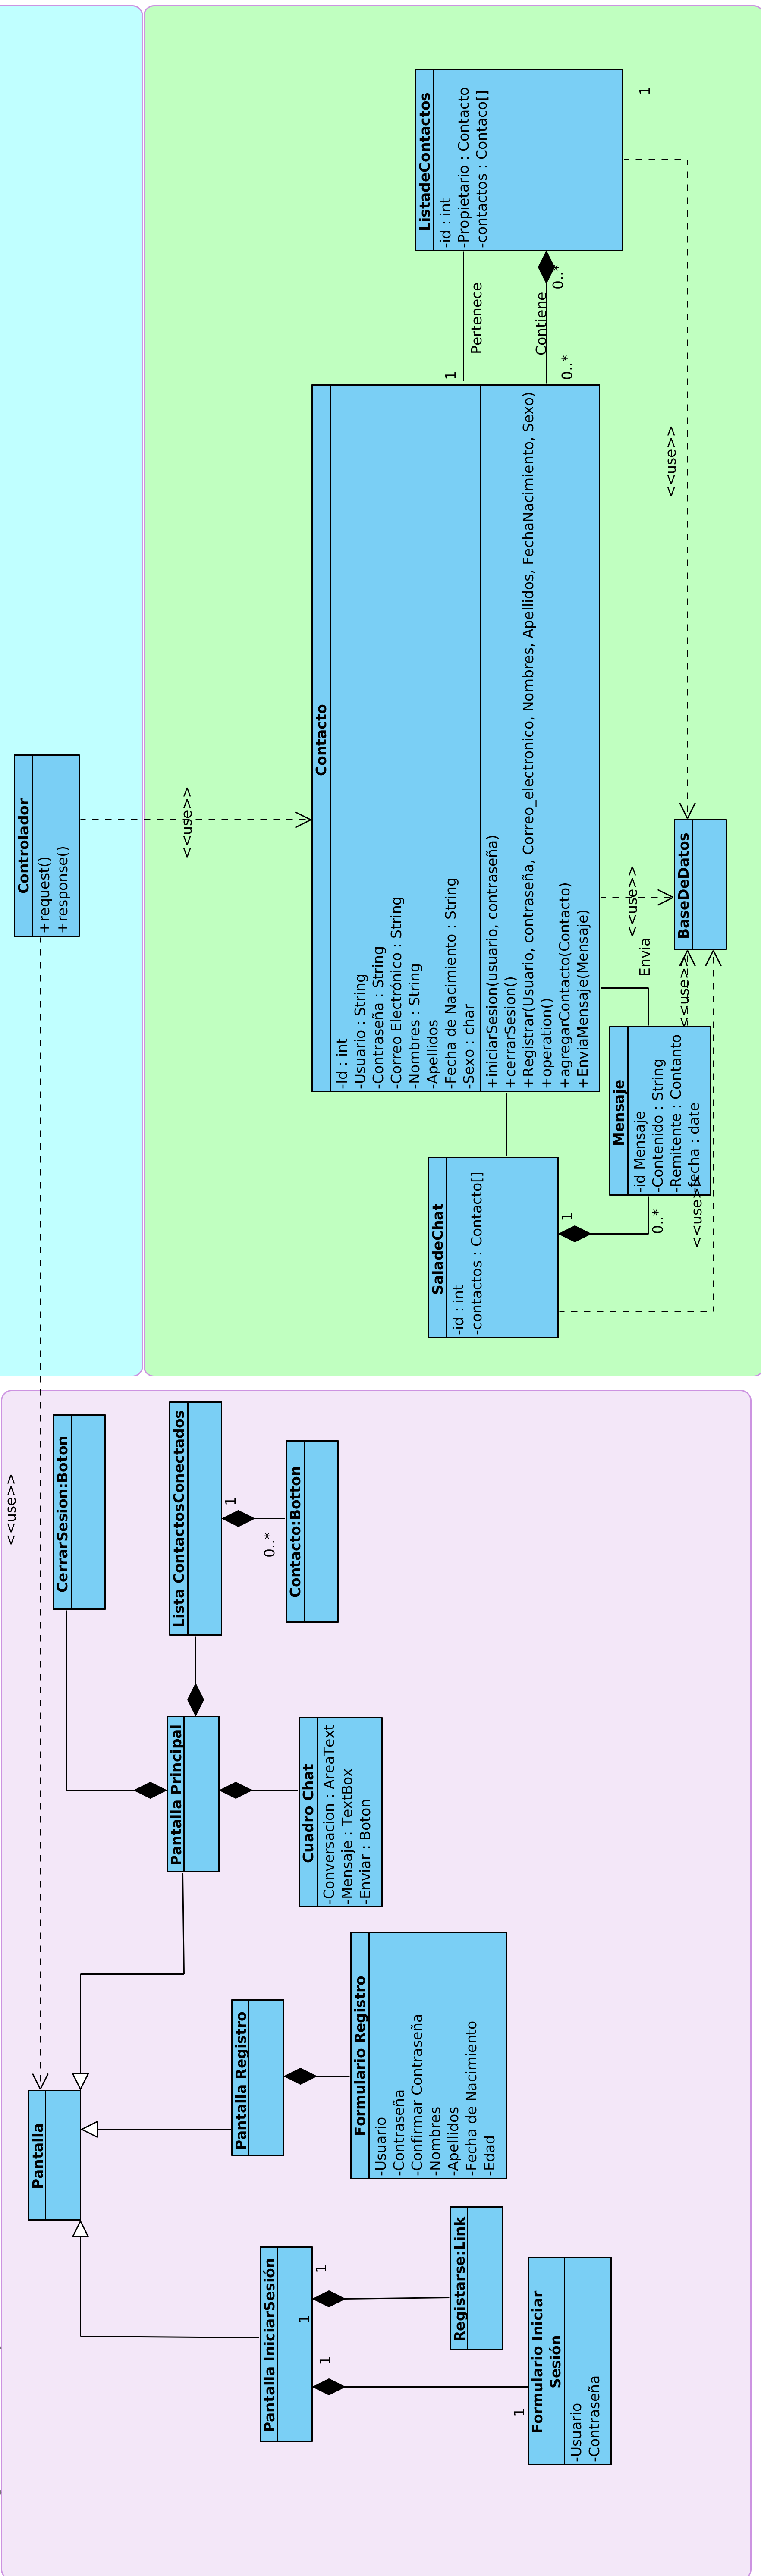
\includegraphics[width=12cm, height=20cm]{images/Diagramas/dclases}
%		\caption{Diagrama de Clases del sistema de mensajer\'ia.}
%	\end{figure}
	
	\begin{figure}[htbp!]
		\centering
			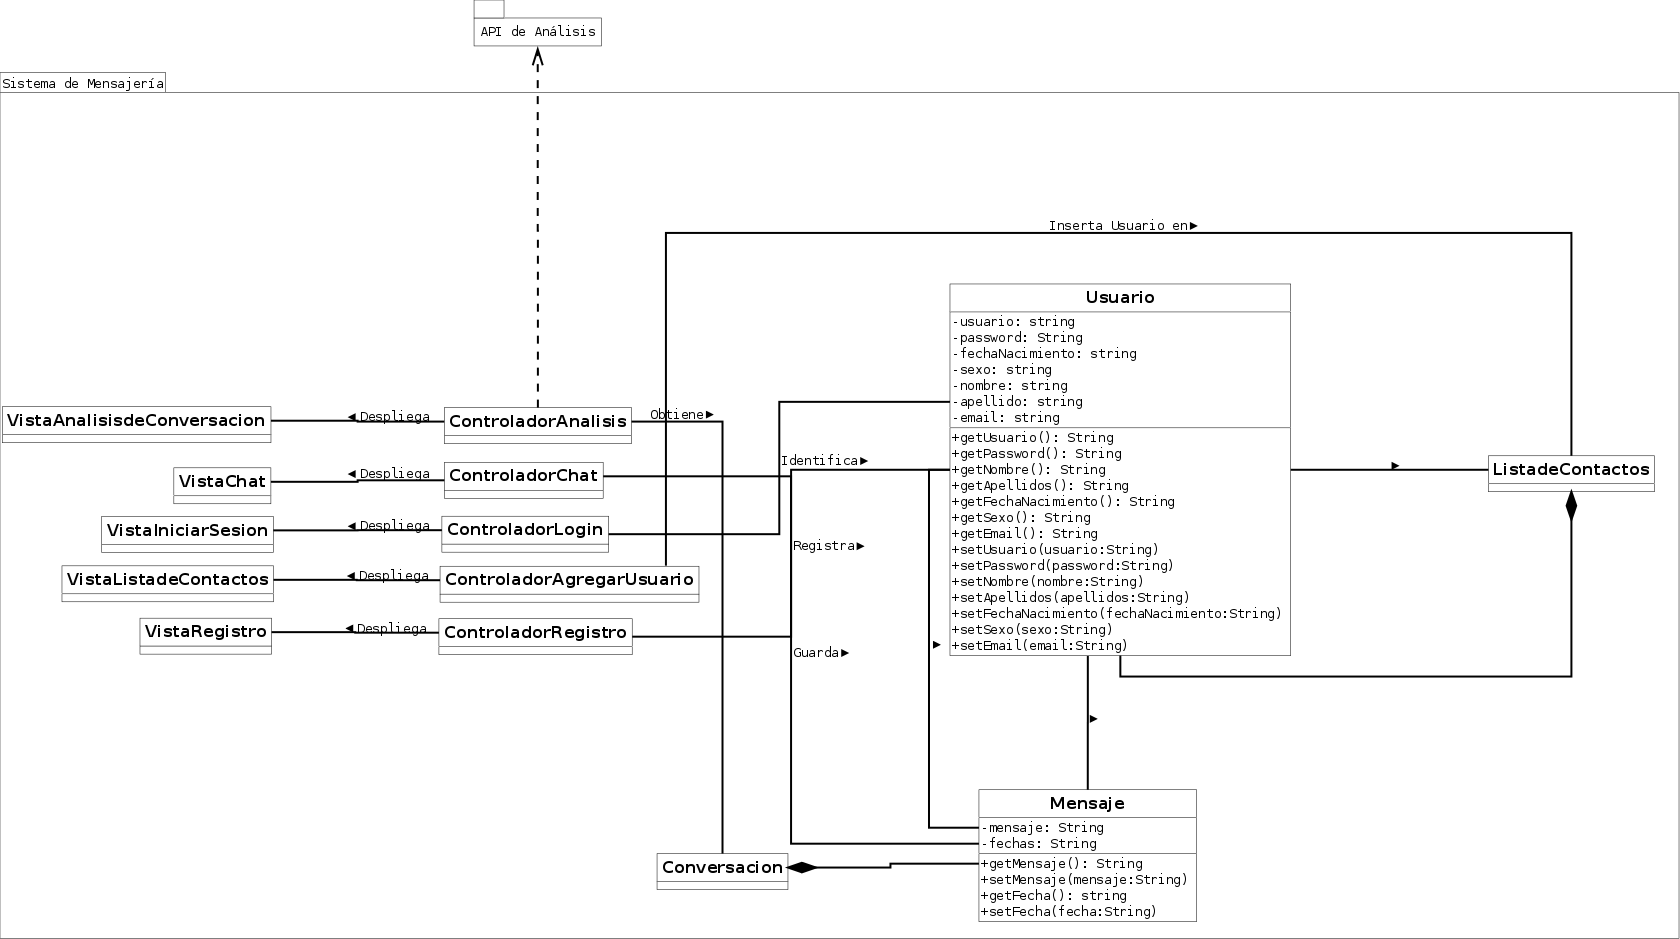
\includegraphics[width=18cm, height=13cm]{images/Diagramas/ddclases}
		\caption{Diagrama de Clases del sistema de mensajer\'ia.}
	\end{figure}
	
	

	
	\pagebreak
%\section{Modelo de la interacci\'on del Contacto con el sistema de mensajer\'ia }
\subsection{Diagrama de secuencia del sistema de mensajer\'ia (Iniciar sesi\'on)}
El siguiente diagrama de secuencia muestra las acciones que realiza el sistema y la interacci\'on que se lleva acabo con el usuario en el momento en el que un Contacto realiza el inicio de sesi\'on.


	\begin{figure}[htbp!]
		\centering
			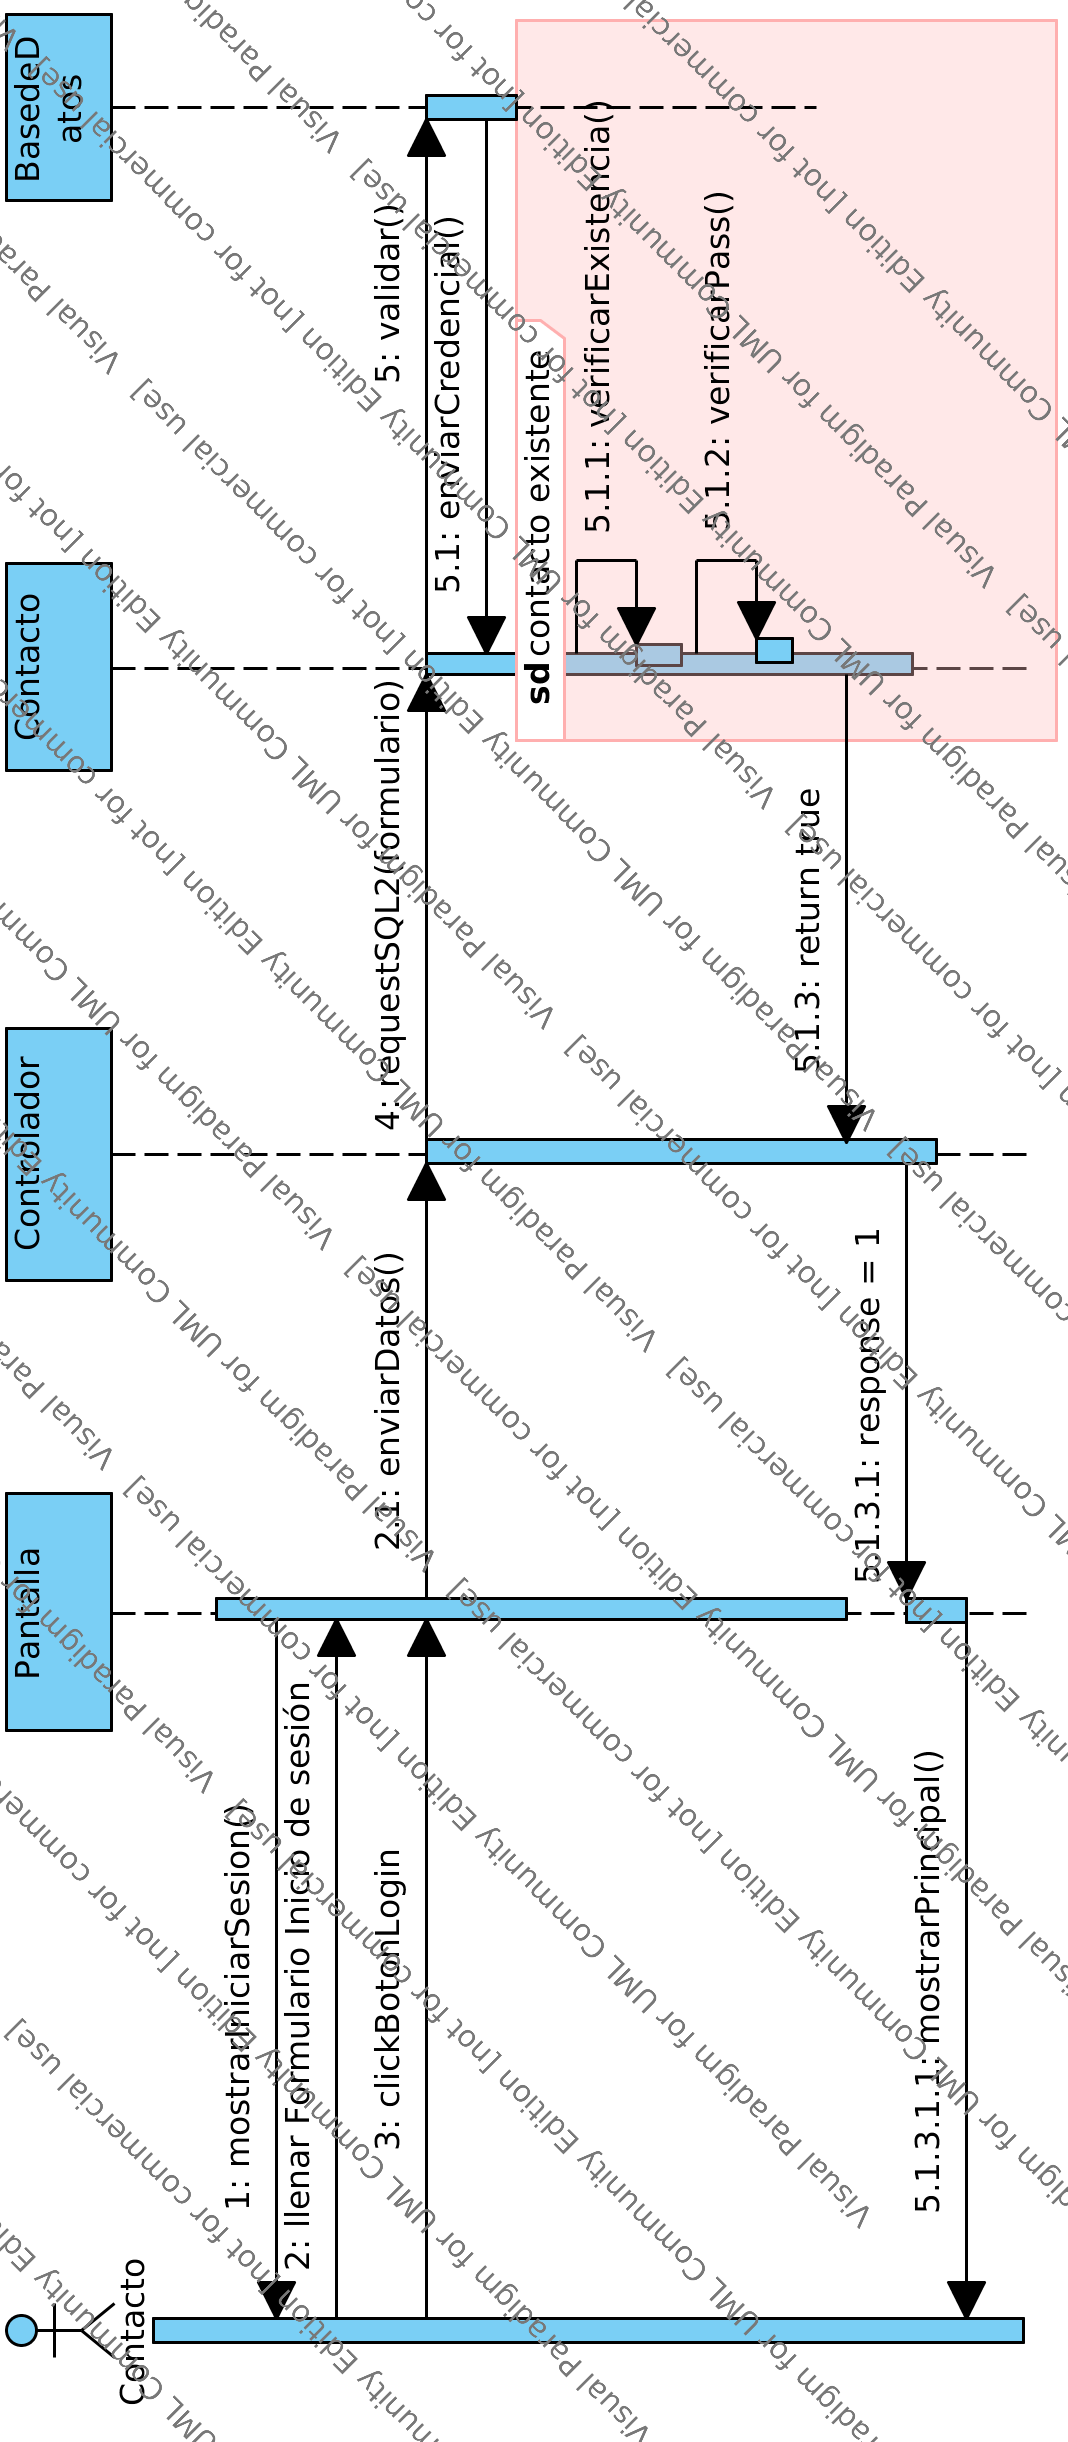
\includegraphics[width=15cm, height=20cm]{images/Diagramas/SecIniciarSesion}
		\caption{Diagrama de Secuencia Iniciar Sesi\'on.}
	\end{figure}
	\pagebreak	
\subsection{Diagrama de secuencia del sistema de mensajer\'ia (Registro de Contacto)}
El siguiente diagrama de secuencia muestra las acciones que realiza el sistema en el momento en el que un usuario nuevo desea registrarse en el sistema para su posterior uso.
	
	
	\begin{figure}[htbp!]
		\centering
			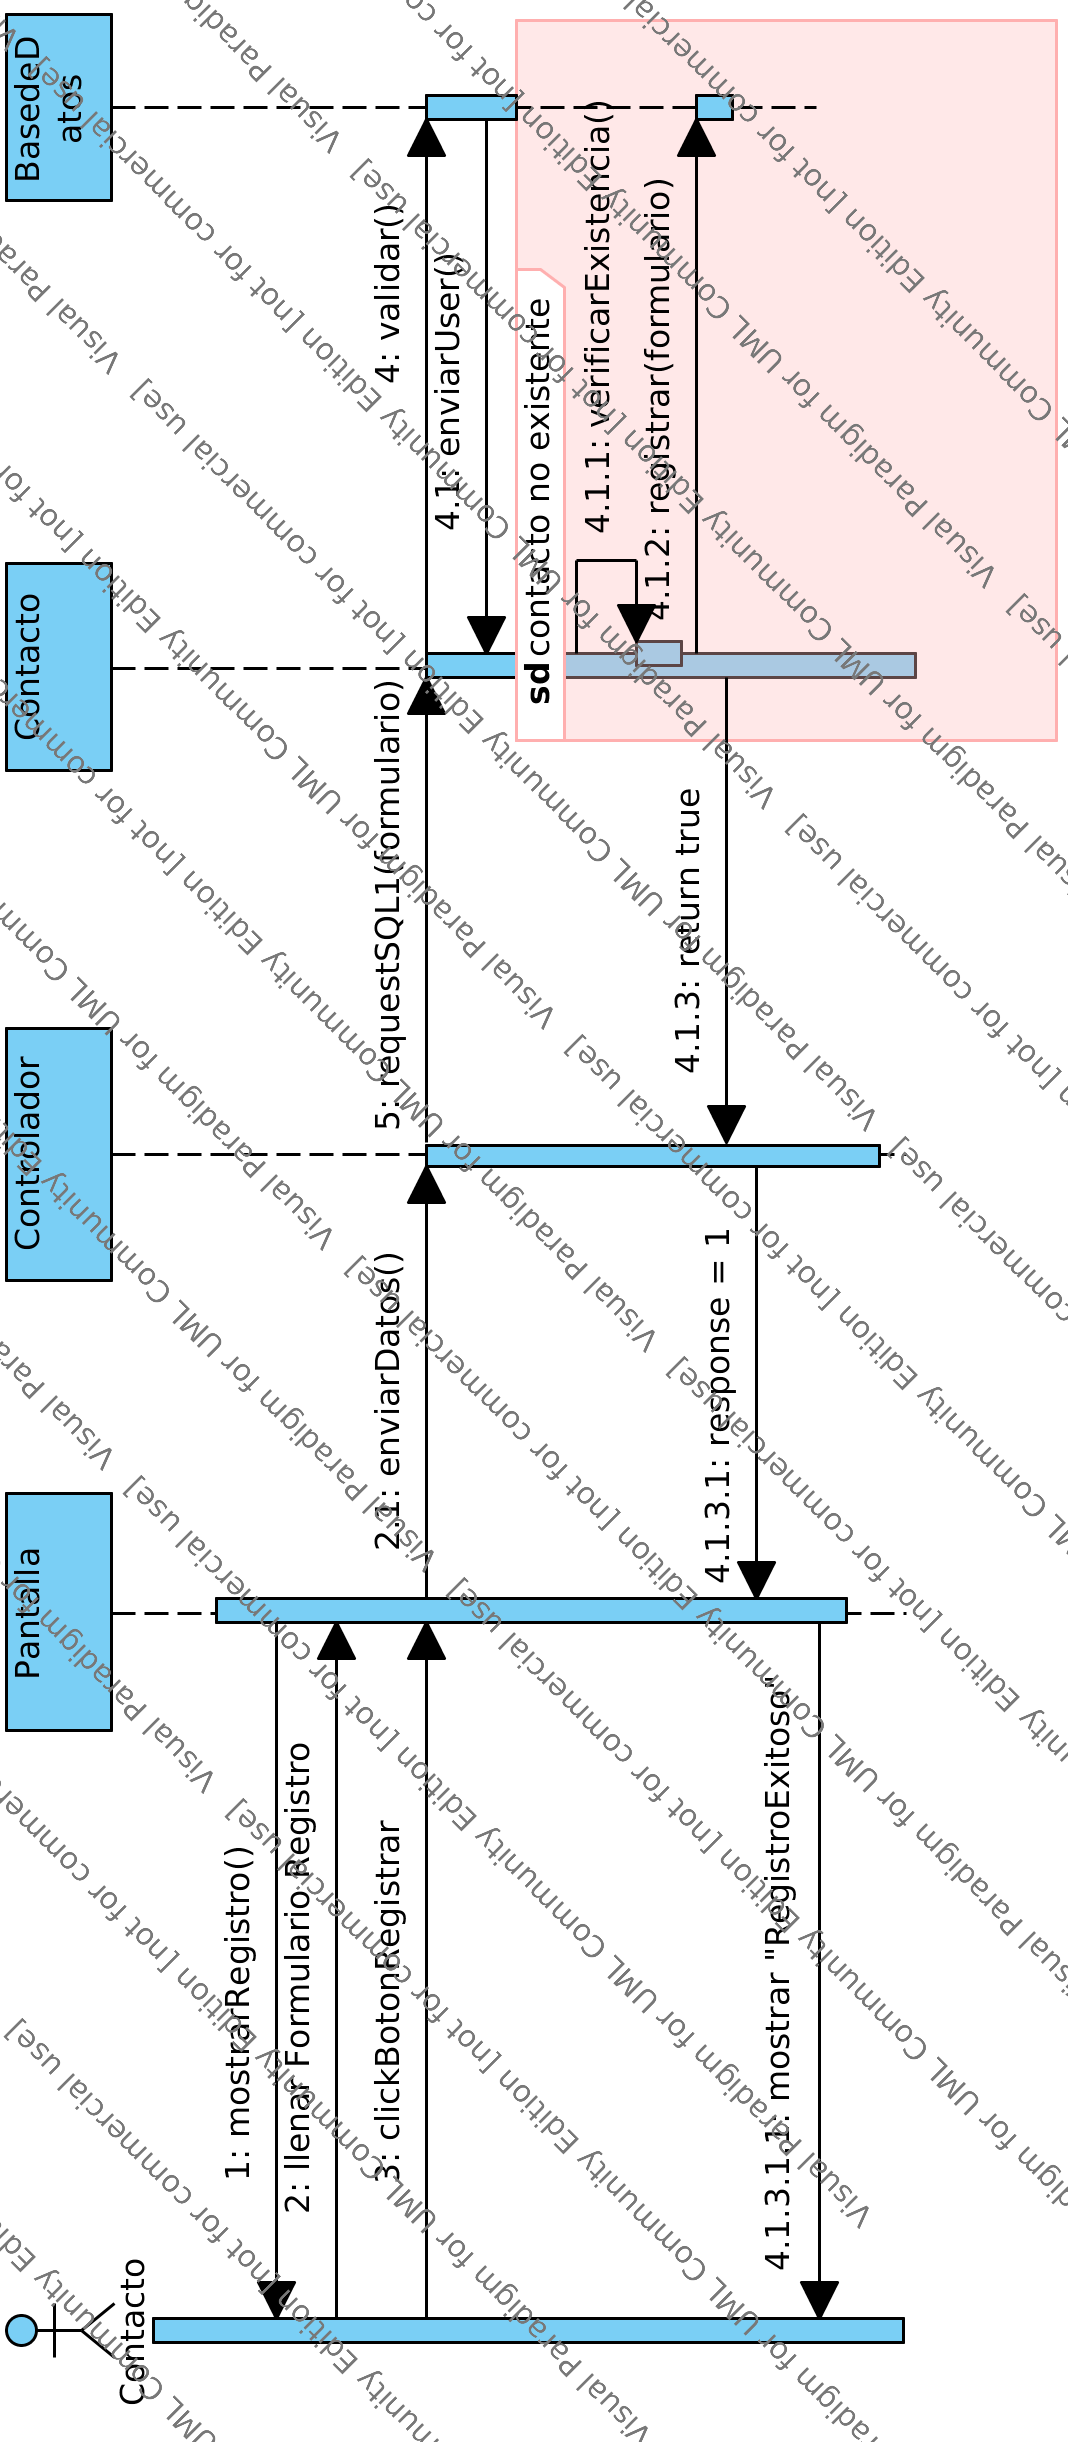
\includegraphics[width=15cm, height=20cm]{images/Diagramas/SecRegistro}
		\caption{Diagrama de Secuencia Registro.}
	\end{figure}
	\pagebreak
\subsection{Diagrama de secuencia del sistema de mensajer\'ia (Agregar Contacto)}
El siguiente diagrama de secuencia muestra las acciones que realiza el sistema cuando un usuario desea agregar a su lista de contactos un nuevo Contacto.
	
	
	\begin{figure}[htbp!]
		\centering
			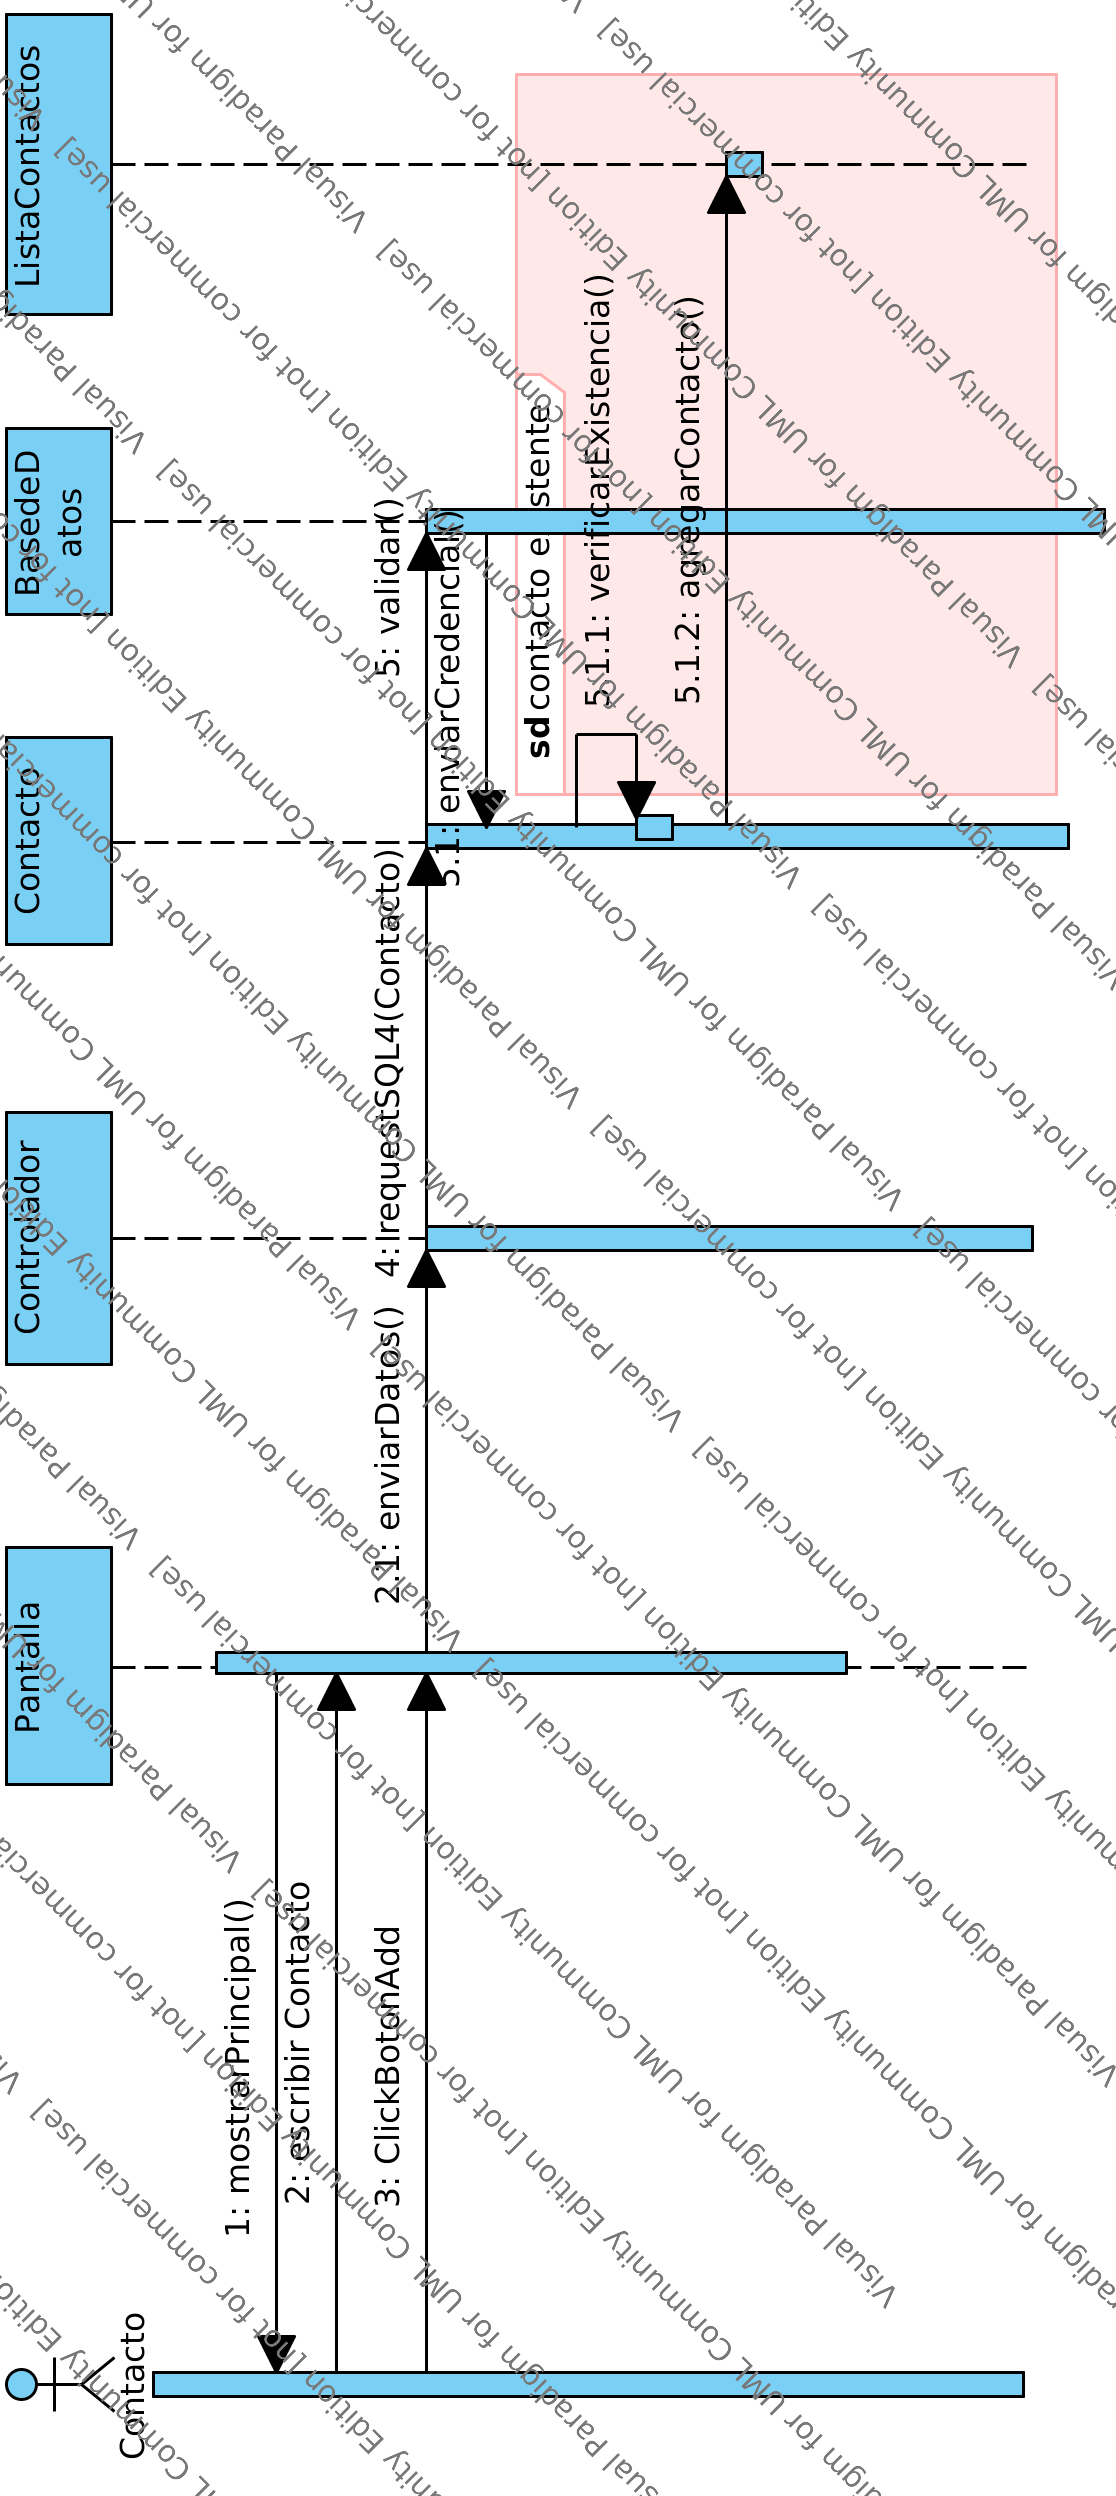
\includegraphics[width=15cm, height=20cm]{images/Diagramas/SecAdd}
		\caption{Diagrama de Secuencia Agregar contacto.}
	\end{figure}
		\pagebreak
\subsection{Diagrama de secuencia del sistema de mensajer\'ia (Enviar mensaje)}
El siguiente diagrama de secuencia muestra los pasos que lleva acabo el sistema en el momento en el que un Contacto decide enviar un mensaje a otro Contacto.
		
		\begin{figure}[htbp!]
		\centering
			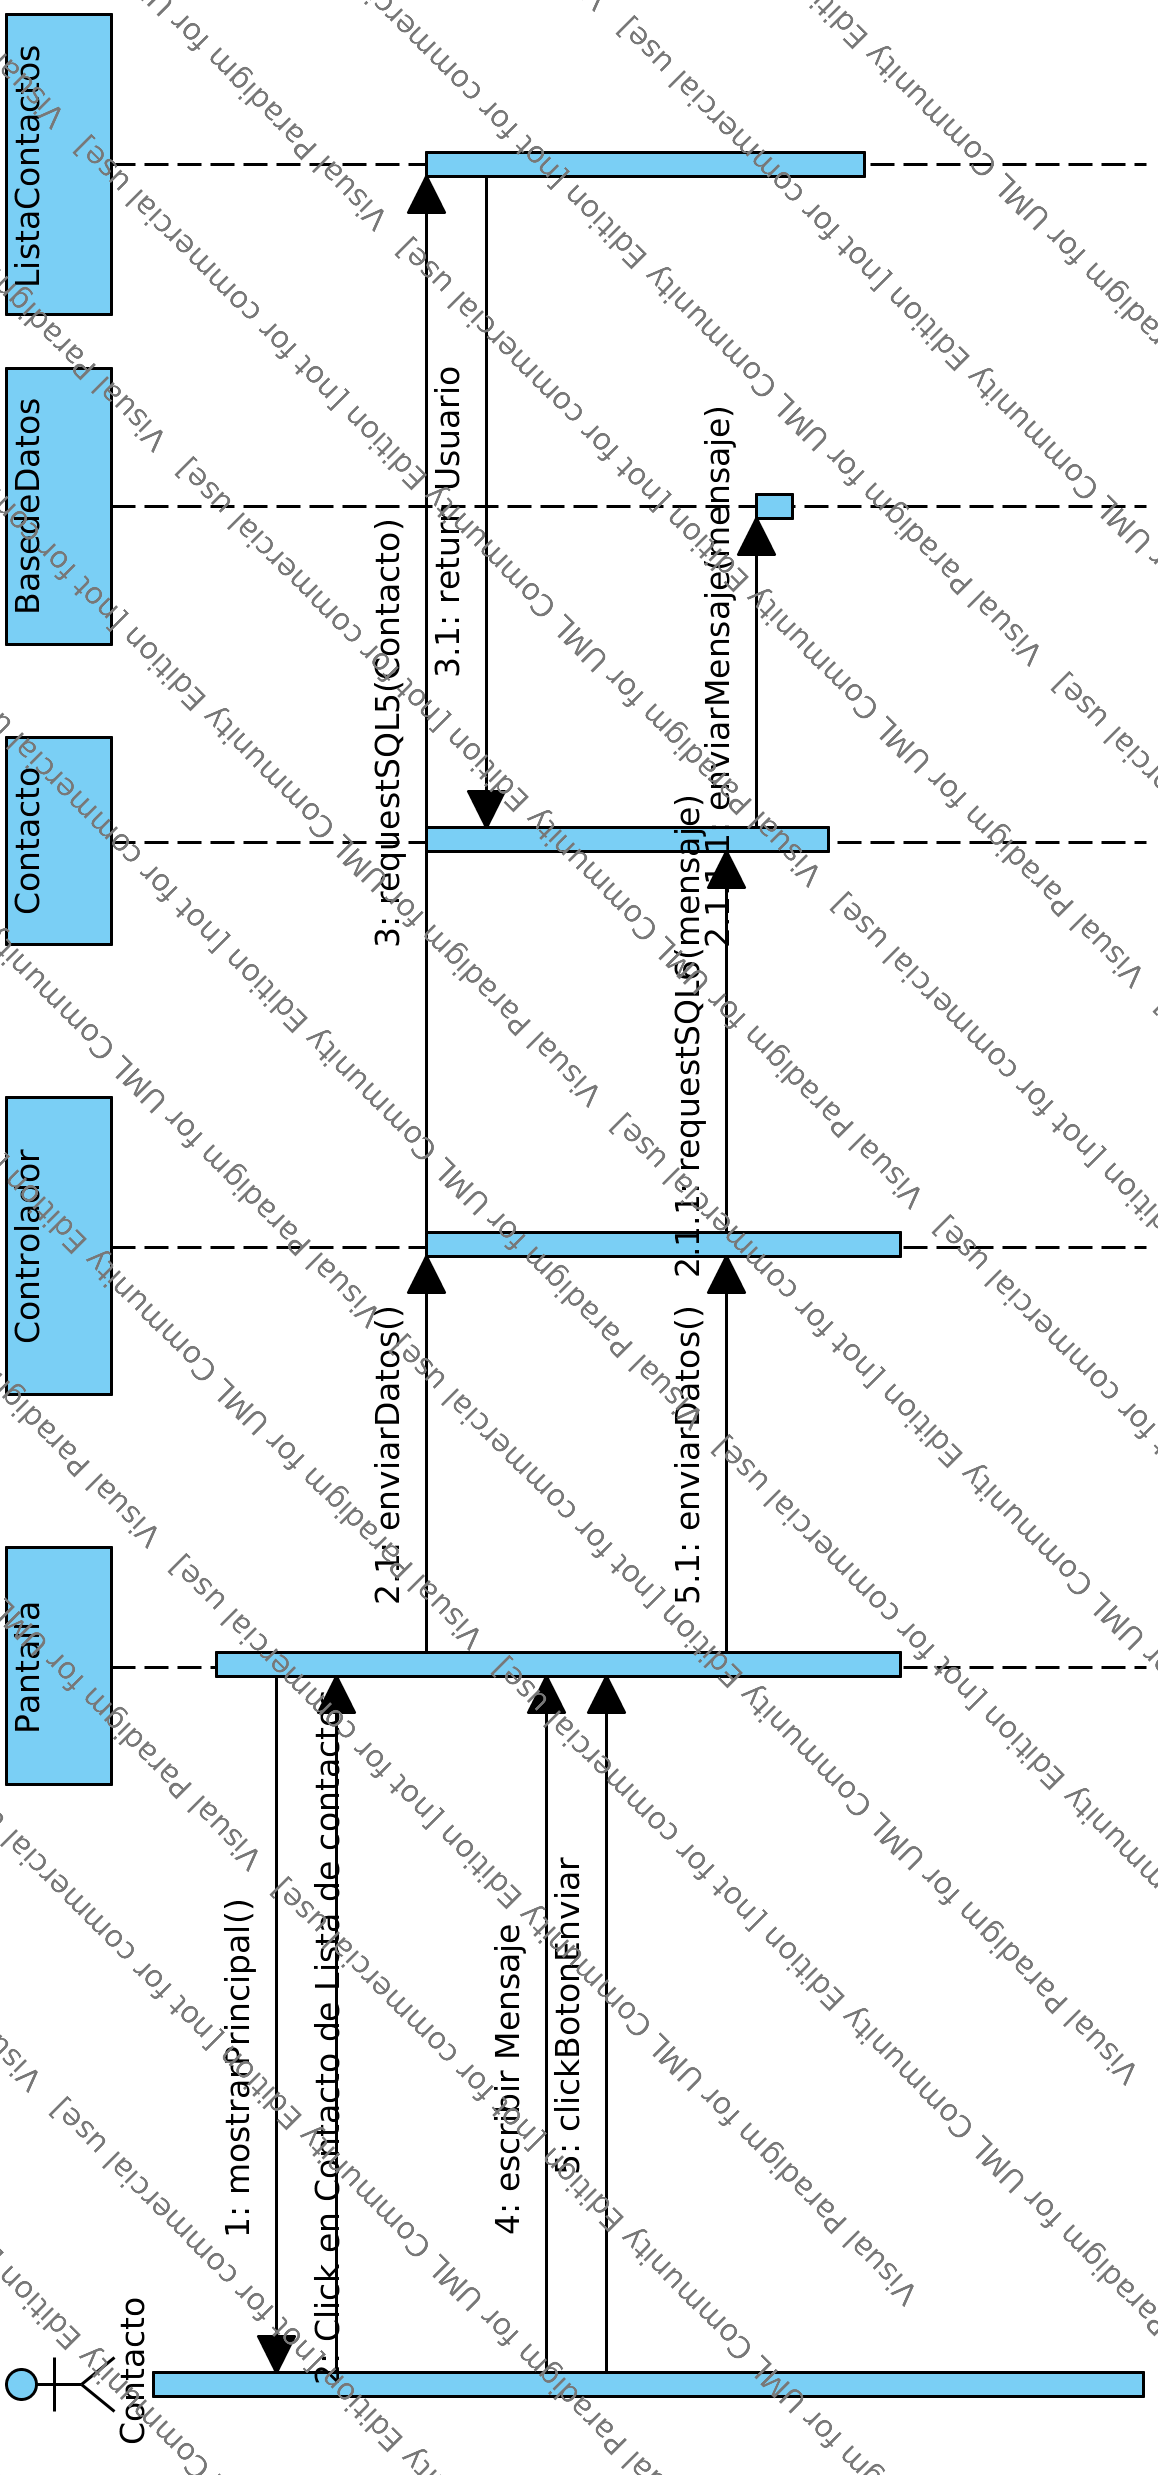
\includegraphics[width=15cm, height=20cm]{images/Diagramas/SecEnviar}
		\caption{Diagrama de Secuencia Enviar Mensaje.}
	\end{figure}
		\pagebreak
	\subsection{Diagrama de secuencia del sistema de mensajer\'ia (Cerrar sesi\'on)}
El siguiente diagrama de secuencia muestra las acciones que realiza el sistema y la interacci\'on que se lleva acabo con el usuario en el momento en el que un Contacto desea cerrar su sesi\'on.
	
			\begin{figure}[htbp!]
		\centering
			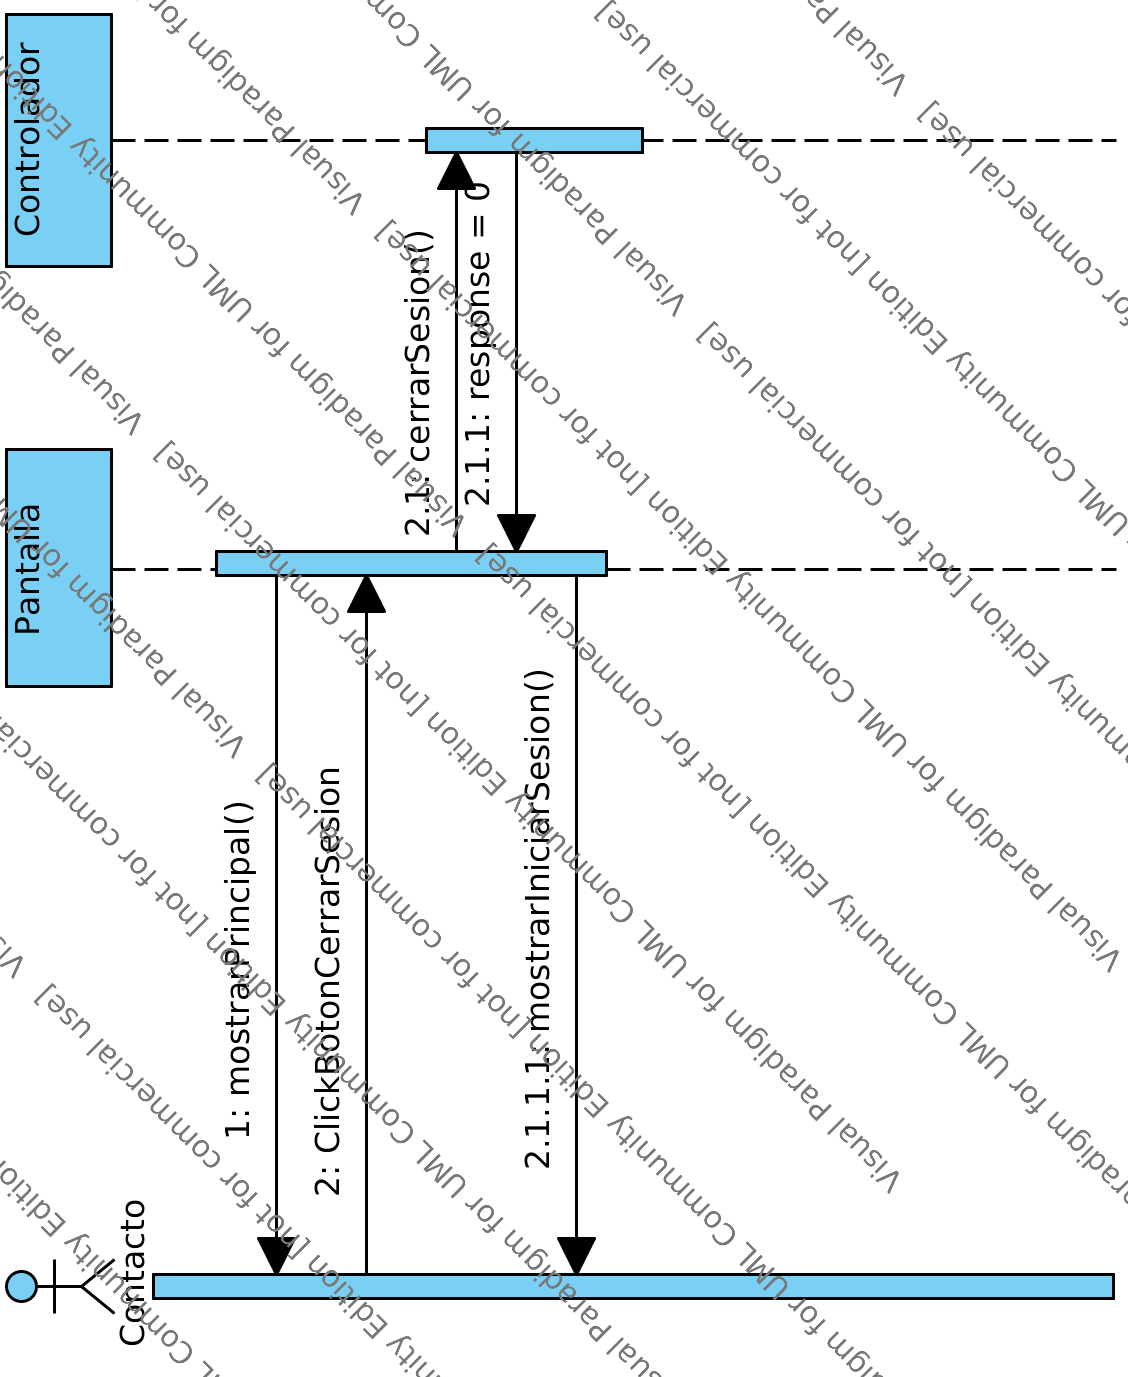
\includegraphics[width=15cm, height=20cm]{images/Diagramas/SecCerrar}
		\caption{Diagrama de Secuencia Cerrar sesi\'on.}
	\end{figure}

	
	\pagebreak
%
		
		\subsection{IU1 Pantalla de Iniciar sesi\'on}

\subsubsection{Objetivo}
	Verificar si el usuario que est\'a intentando entrar al sistema sea el correcto y ya se encuentra registrado en el sistema de mensajer\'ia.

\subsubsection{Dise\~no}
	Esta pantalla aparece al ingresar al sistema de mensajer\'ia. 

	\begin{figure}[htbp!]
		\centering
			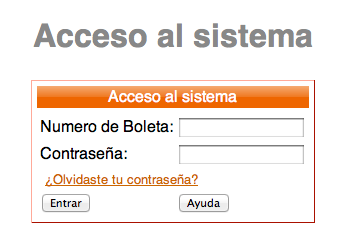
\includegraphics[width=0.9\textwidth]{images/Modulo1/Login}
		\caption{Pantalla de inicio de sesi\'on.}
	\end{figure}

\subsubsection{Salidas}
Ninguna


\subsubsection{Entradas}
\begin{Citemize}

\item Usuario 
\item Contrase\~na
\end{Citemize}

\subsubsection{Comandos}
\begin{itemize}
	\item \IUbutton{Login}: Verifica que el usuario se encuentre registrado en la base de datos y de ser as\'i verifica que la contrase\~na corresponda al usuario. 
	\item \IUbutton{Reg\'istrate}: Muestra el formulario que el usuario necesita llenar para poder registrarse en el sistema.
\end{itemize}

\subsubsection{Mensajes}
	\begin{Citemize}
		\item {\bf MSG1} Forbidden.	\end{Citemize}
		
	\pagebreak		%%%%%%%%%%%%%%%%%%%%%%%%%%%%%%%%%%%%%%%%%%%%%%%%%%
		
		\subsection{IU2 Pantalla de Registro de usuario}

\subsubsection{Objetivo}
	Registrar a un usuario con el objetivo de obtener sus datos principales y que \'este posteriormente pueda hacer uso del sistema de mensajer\'ia.

\subsubsection{Dise\~no}
	Esta pantalla aparece al dar clic en el bot\'on \IUbutton{Registrarte} que se encuentra al final de la pantalla de inicio.

	\begin{figure}[htbp!]
		\centering
			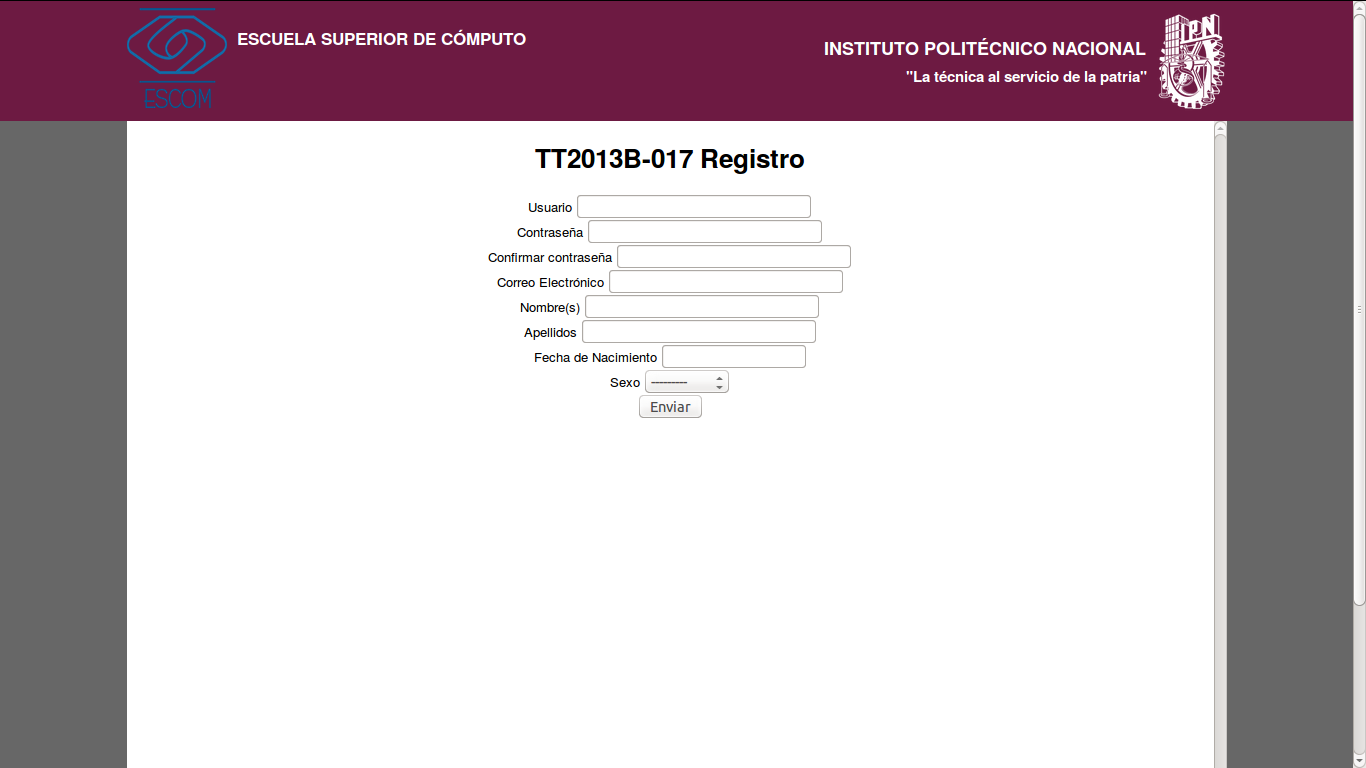
\includegraphics[width=0.8\textwidth]{images/Modulo1/Registro}
		\caption{Pantalla de registro de usuario.}
	\end{figure}

\subsubsection{Salidas}
	\begin{Citemize}
		\item {\bf MSG1} Ha sido registrado correctamente.	
	\end{Citemize}
	


\subsubsection{Entradas}
\begin{Citemize}

\item Usuario 
\item Contrase\~na
\item Correo electr\'onico 
\item Nombre
\item Apellidos
\item Fecha de nacimiento
\item Sexo
\end{Citemize}

\subsubsection{Comandos}
\begin{itemize}
	\item \IUbutton{Enviar}: Ingresa los datos del usuario a la base de datos, si estos fueron ingresados correctamente muestra el mensaje de registro exitoso. \end{itemize}
	\begin{figure}[htbp!]
		\centering
			
\includegraphics[width=0.9\textwidth]{images/Modulo1/SalidaRegistro}
		\caption{Mensaje de registro exitoso.}
	\end{figure}
\subsubsection{Mensajes}
	\begin{Citemize}
		\item {\bf MSG2} This field is required.	\end{Citemize}
		
			\pagebreak%%%%%%%%%%%%%%%%%%%%%%%%%%%%%%%%%%%%%%%%%%%%%%%%%%
	\subsection{IU3 Pantalla de Conversaciones}

\subsubsection{Objetivo}
	El objetivo de esta pantalla es que el usuario pueda visualizar las conversaciones que tiene, es decir, los contactos que forman parte de su lista.

\subsubsection{Dise\~no}
	Esta pantalla aparece al iniciar sesi\'on correctamente.

	\begin{figure}[htbp!]
		\centering
			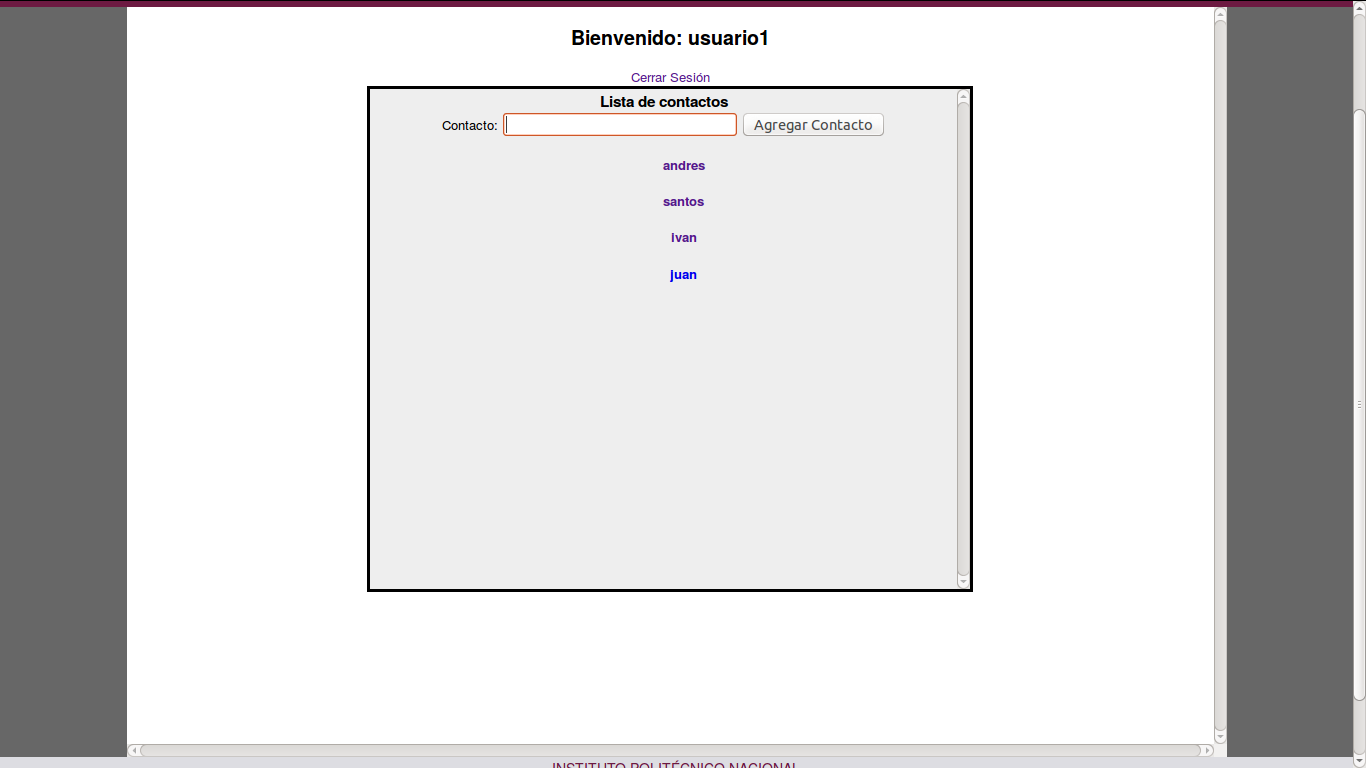
\includegraphics[width=0.9\textwidth]{images/Modulo1/Conversaciones}
		\caption{Pantalla de conversaciones}
	\end{figure}

\subsubsection{Salidas}
Lista de Contactos (conversaciones)


\subsubsection{Entradas}
\begin{Citemize}


\item Contacto
\end{Citemize}
\subsubsection{Comandos}
\begin{itemize}
			\item \IUbutton{"Contacto"}: Muestra la conversaci\'on del Contacto seleccionado y permite el intercambio de mensajes.
			\item \IUbutton{Cerrar sesi\'on}: Termina la sesi\'on y regresa a la p\'agina de inicio.
	\end{itemize}

\subsubsection{Mensajes}
Ninguno

		
	\pagebreak		%%%%%%%%%%%%%%%%%%%%%%%%%%%%%%%%%%%%%%%%%%%%%%%%%%
	
	
	
		
		\subsection{IU4 Pantalla del Sistema de Mensajer\'ia}

\subsubsection{Objetivo}
	El objetivo de esta pantalla es que el usuario pueda enviar y recibir mensajes de otros usuarios conectados.

\subsubsection{Dise\~no}
	Esta pantalla aparece al elegir el Contacto con el cual se desea intercambiar mensajes o analizar conversaciones pasadas.

	\begin{figure}[htbp!]
		\centering
			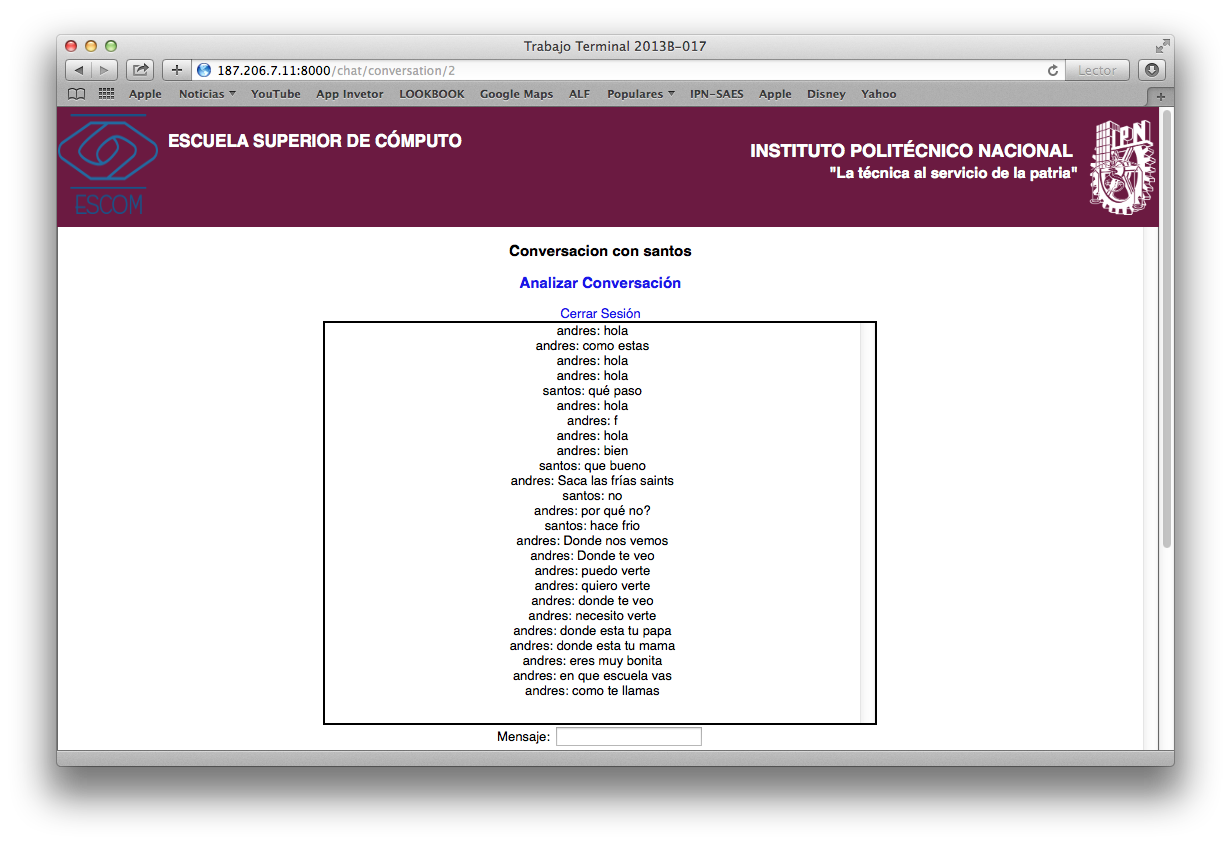
\includegraphics[width=0.9\textwidth]{images/Modulo1/Chat}
		\caption{Pantalla del sistema de mensajer\'ia}
	\end{figure}

\subsubsection{Salidas}
Conversaci\'on


\subsubsection{Entradas}
\begin{Citemize}

\item Mensaje 

\end{Citemize}
\subsubsection{Comandos}
\begin{itemize}
	\item \IUbutton{Enviar Mensaje}: Se env\'ia la cadena de caracteres contenida en el campo "Mensaje" a otro usuario del sistema. 
	\item \IUbutton{Analizar Conversaci\'on}: Muestra el an\'alisis de la conversaci\'on actualmente mostrada.
		\item \IUbutton{Cerrar sesi\'on}: Termina la sesi\'on y regresa a la p\'agina de inicio.
	\end{itemize}

\subsubsection{Mensajes}
Ninguno




	\pagebreak%%%%%%%%%%%%%%%%%%%%%%%%%%%%%%%%%%%%%%%%%%%%%%%%%%

	
	
	
	
			\subsection{IU5 Pantalla del An\'alisis (Gr\'afica)}

\subsubsection{Objetivo}
	El objetivo de esta pantalla es que el usuario pueda visualizar los resultados del an\'alisis realizado a la conversaci\'on solicitado.

\subsubsection{Dise\~no}
	Esta pantalla aparece despu\'es de solicitar el an\'alisis de la conversaci\'on en la pantalla del chat.

	\begin{figure}[htbp!]
		\centering
			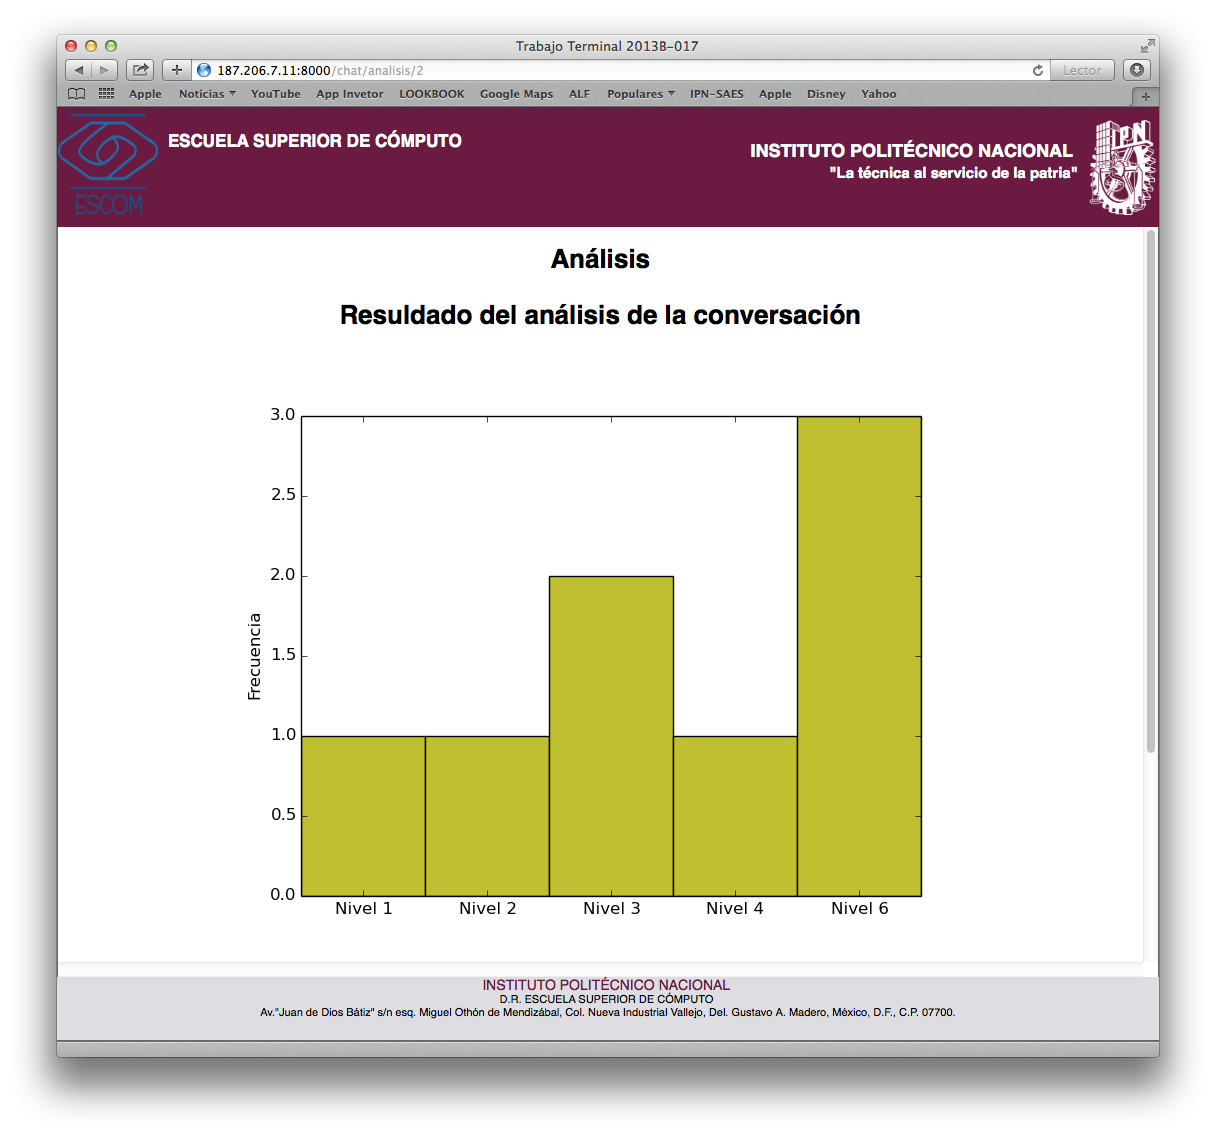
\includegraphics[width=0.9\textwidth]{images/Modulo1/GraficaAnalisis}
		\caption{Pantalla del An\'alisis (Gr\'afica)}
	\end{figure}

\subsubsection{Salidas}
Ninguna


\subsubsection{Entradas}
Ninguna
\subsubsection{Comandos}
Ninguno
\subsubsection{Mensajes}
Resultados del an\'alisis de la conversaci\'on 

\begin{figure}[htbp!]
		\centering
			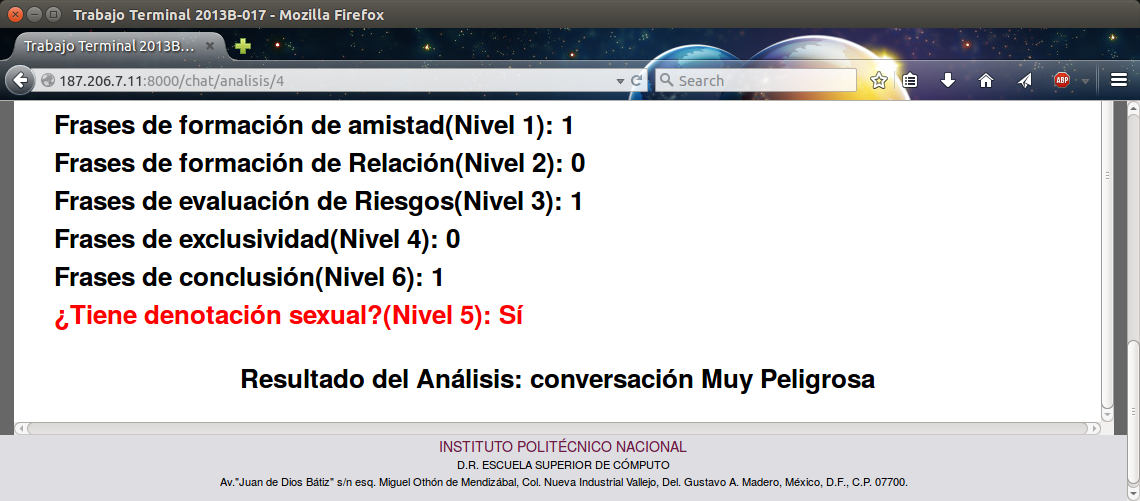
\includegraphics[width=0.9\textwidth]{images/Modulo1/InsidenciasNivel}
		\caption{Pantalla del An\'alisis (Incidencias)}
	\end{figure}



	\pagebreak%%%%%%%%%%%%%%%%%%%%%%%%%%%%%%%%%%%%%%%%%%%%%%%%%%



%=========================================================
%=========================================================

\chapter{Prototipo 1: Identificador y clasificador de frases del online grooming}
\section{Marco Te\'orico del prototipo}

\subsection{Online Grooming}
El online Grooming es un fen\'omeno que podr\'iamos traducir como engatusamiento y que se utiliza para describir las pr\'acticas online de ciertos adultos para ganarse la confianza de un (o una) menor fingiendo empat\'ia, cariño, etc. con fines de satisfacción sexual (como m\'inimo, y casi siempre, obtener im\'agenes del menor desnudo o realizando actos sexuales).

Por tanto est\'a muy relacionado con la pederastia y la pornograf\'ia infantil en Internet. De hecho el grooming es en muchas ocasiones la antesala de un abuso sexual \cite{grooming}.

\subsection{Caracterización del online grooming}
De acuerdo a las conversaciones analizadas por los Doctores Aditi Gupta, Ponnurangam Kumaraguru, Ashish Surekason del Instituto Tecnol\'ogico de Informaci\'on en la India reportadas en el art\'iculo  ``Characterizing pedophile conversations on the Internet using Online Grooming Web.'' \cite{articulo}, identificaron una serie de etapas y estados que las  las conversaciones pueden atravesar. Los autores marcan 6 etapas principales las cuales se describen en la tabla \ref{table:caracterizacion}.


\begin{table}[!h]

\begin{tabular}[t]{|p{15mm} |p{22mm} |p{22mm} |p{22mm} |p{20mm} |p{20mm} |p{20mm} |}
\hline
\hline
Etapas & Formaci\'on de la amistad & Formaci\'on de una relaci\'on & Evaluaci\'on de riesgos & Exclusividad & Sexual & Conclusi\'on \\
\hline
Descriptor1 & Intercambio de cuentas de correo electr\'onico, fotograf\'ias, webcam, informaci\'on & Intercambio de cuentas de correo electr\'onico, fotograf\'ias, webcam, informaci\'on & Evaluar a los padres del ni\~no, si est\'an alrededor o qui\'en puede ver su computadora & Sentir amor y expresar exclusividad & Dar descripci\'on del cuerpo y la figura & Quedar un d\'ia, una cita, hora, lugar para conocerse en persona \\
\hline
Descriptor2 &Hablar de novios/novias & Dar suaves cumplidos & Pedir al ni\~no eliminar su historial de conversaciones, asegurarse quenadie tenga la contrase\~na & Describir actividad sexual y experiencias al ni\~no &Ser novios &Discutir puntos en com\'un para una reuni\'on \\
\hline
Descriptor3 &Obtener informaci\'on del perfil y otras cuentas del ni\~no & hablar de los hobbies del a\~no, actividades e intereses & Ver si el ni\~no est\'a c\'omodo con ver a alguien mayor& Cumplidos fuertes & Intercambiar fotograf\'ias sexuales & Asegurarse de que el ni\~no ir\'a s\'olo \\
\hline
Descriptor4 & Preguntar la edad, g\'enero, localidad, nombre, informaci\'on personal, detalles familiares & Escuela, grado, tareas, n\'umero de celular & Asegurarse de que el ni\~no no es un polic\'ia & Construir confianza entre el ni\~no y el ped\'ofilo & Dar orientaci\'on sexual, cumplidos & Decidir qu\'e hacer cuando se conozcan\\
\hline
\end{tabular} \\ \\ \\
\caption{Tabla de caracterizaci\'on del comportamiento de conversaciones peligrosas}
\label{table:caracterizacion}
\end{table}

%Con base a la tabla de caracterizacion del comportamiento de las conversaciones se propuso un conjunto de frases de acuerdo a la etapa que 
%A partir de la observaci\'on de las conversaciones y de acuerdo con la descripci\'on de la matriz se listan las siguientes frases, las cuales marcan un punto de inter\'es en la identificaci\'on de los niveles 1, 2, 3, 4 y 6:





Hacemos menci\'on del nivel 5 cuya caracter\'istica es la descripci\'on sexual de las conversaciones. Este nivel ser\'a evaluado por separado en el prototipo n\'umero 2 ya que el contexto sexual da un peso mayor en la desici\'on de la API.
\textbf{•}

\section{Descripci\'on}
Prototipo que identifica y cuenta frases pertenecientes a los niveles de  formaci\'on de la amistad, formaci\'on de una relaci\'on, evaluaci\'on de riesgos, exclusividad y conclusi\'on de la caracterizac\'on del online grooming.

\section{Objetivo}
Desarrollar un prototipo que procese conversaciones de texto para buscar y contar las frases de los niveles de formaci\'on de la amistad, formaci\'on de una relaci\'on, evaluaci\'on de riesgos, exclusividad y conclusi\'on descritas en la tabla de caracterizac\'on del online grooming.


\section{An\'alisis}
\subsection{Caracter\'isticas}

\begin{description}
\item[FEAT1:] El sistema realiza la b\'usqueda de frases del nivel de formaci\'on de amistad.
\item[FEAT2:] El sistema raliza el conteo de frases del nivel de formaci\'on de amistad.
\item[FEAT3:] El sistema realiza la b\'usqueda de frases del nivel de formaci\'on de una relaci\'on.
\item[FEAT4:] El sistema raliza el conteo de frases del nivel de formaci\'on de una relaci\'on.
\item[FEAT5:] El sistema realiza la b\'usqueda de frases del nivel de evaluaci\'on de riesgos.
\item[FEAT6:] El sistema raliza el conteo de frases del nivel evaluaci\'on de riesgos.
\item[FEAT7:] El sistema realiza la b\'usqueda de frases del nivel de exclusividad.
\item[FEAT8:] El sistema raliza el conteo de frases del nivel de exclusividad.
\item[FEAT9:] El sistema realiza la b\'usqueda de frases del nivel de conclusi\'on.
\item[FEAT10:] El sistema raliza el conteo de frases del nivel conclusi\'on.
\end{description}

\subsection{Restricciones}
\begin{itemize}
\item Conversaciones alamacenadas en archivos de texto planos.
\item Conversaciones almacenadas en archivos con formato XML.
\item Implementaci\'on del prototipo en python.

\end{itemize}

\section{Dise\~no}

La figura \ref{fig:arquitectura_prototipo1} muestra la arquitectura del prototipo. Tal como se muestra en el diagrama, la entrada de informaci\'on del prototipo son los archivos que contienen a las conversaciones. La salida del prototipo ser\'an los valores del n\'umero de frases correspondientes a cada nivel de caracterizaci\'on del Online grooming. Estos valores ser\'an almacenados en una base da datos para su posterioir procesamiento y análisis.



	\begin{figure}[!h]
	\begin{center}
	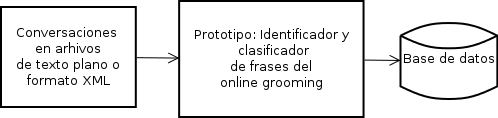
\includegraphics[scale=.5]{images/arquitectura_prototipo1}
	\caption{Arquitectura del prototipo 1}
	\label{fig:arquitectura_prototipo1}
	\end{center}
	\end{figure}


\subsection{Diagrama de Clases}


La figura \ref{fig:diagramaDeClase} muestra el diagrama de la clase que conforma el prototipo. Los atributos de cada clase representan el n\'umero de frases que la conversaci\'on tiene en el nivel que describe.
\begin{figure}[h]
	\begin{center}
	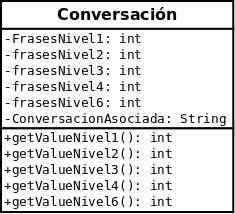
\includegraphics[scale=.4]{images/claseprotipo2}
	\caption{Diagrama de Clase del prototipo 1}
	\label{fig:diagramaDeClase}
	\end{center}
	\end{figure}



\subsection{M\'etodo para la identificaci\'on y conteo de frases del nivel de formaci\'on de amistad}
La siguiente lista de frases pertenecen al nivel de formaci\'on de amistadad cuyo objetivo es establecer confianza y obtener datos de la v\'ictima. Estas frases se seleccionaron de acuerdo a las posibles frases que se pod\'ian formar de acuerdo a los descriptores que la tabla de caracterizac\'on muestra.

\begin{itemize}
\item ?`C\'omo te llamas?
\item ?`C\'ual es tu nombre?
\item ?`Cu\'antos a\~nos tienes?
\item ?`D\'onde vives?
\item ?`Qu\'e m\'usica te gusta?
\end{itemize}


El siguiente c\'odigo muestra mediante la cual detectamos las frases que corresponden al nivel 1. Para hacer la b\'usqueda se toman palabras clave como palabras anclas y as\'i poder encontrar no s\'olo la frase escrita integramente sino que tambi\'en se puedan identificar algunos de sus derivados.

\begin{lstlisting}[language=Python]
def detectarNivel1(self):	
		for mensaje in self.mensajes:
			#Contexto busqueda de la edad
			if (u'cuantos' in mensaje) == True:
				if(u'anos' in mensaje) == True:
					if(u'tienes' in mensaje) == True:
				#		print mensaje
						self.nivel1 += 1
	
			if(u'cual' in mensaje) == True:
				if(u'edad' in mensaje) == True:
				#	print mensaje
					self.nivel1 += 1
			#Contexto busqueda nombre
			if(u'como' in mensaje) == True:
				if(u'llamas' in mensaje) == True:
				#	print mensaje
					self.nivel1 += 1
			if(u'cual' in mensaje) == True:
				if(u'nombre' in mensaje)== True:
				#	print mensaje
					self.nivel1 += 1
			if(u'donde' in mensaje) ==  True:
				if(u'vives' in mensaje) == True:
				#	print mensaje
					self.nivel1 += 1
			if(u'musica' in mensaje) == True:
					self.nivel1 += 1
			if(u'escuchar' in mensaje) == True:
					self.nivel1 += 
\end{lstlisting}



\subsection{Lista de frases de nivel formaci\'on de una relaci\'on}
La siguiente lista de frases son frases que pertenecen al nivel de formaci\'on de una relaci\'on de la tabla de caracterizaci\'on del online grooming, cuyo objetivo es establecer amistad con la v\'ictima. 
Las frases fueron propuestas de acuerdo a los descriptores que el nivel marca.

\begin{itemize}
\item ?`Tienes Fotos?
\item ?`Tienes webcam?
\item ?`En qu\'e escuela vas?
\item ?`Cu\'al es tu celular?
\item ?`Cu\'al es tu tel\'efono?
\item ?`Cu\'al es tu n\'umero telef\'onico?
\end{itemize}

\begin{lstlisting}[language=Python]
def detectarNivel2(self):
		stemmer = SnowballStemmer("spanish")
		for mensaje in self.mensajes:
			for palabra in mensaje:
				#Contecto fotos
				if stemmer.stem(palabra) == stemmer.stem("tienes"):
					for palabra2 in mensaje:
						if stemmer.stem(palabra2) == stemmer.stem("fotos"):
				#			print mensaje
							self.nivel2 += 1
				
					for palabra2 in mensaje:
						if stemmer.stem(palabra2) == stemmer.stem("camara"):
				#			print mensaje
							self.nivel2 += 1
					
					for palabra2 in mensaje:
						if stemmer.stem(palabra2) == stemmer.stem("webcam"):
				#			print mensaje
							self.nivel2 += 1
					
					for palabra2 in mensaje:
						if stemmer.stem(palabra2) == stemmer.stem("celular"):
						#	print mensaje	
							self.nivel2 += 1
				#Contexto Escuela
				elif stemmer.stem(palabra) == stemmer.stem("escuela"):
				#	print mensaje
					self.nivel2 +=1		
				elif stemmer.stem(palabra) == stemmer.stem("cual"):	
					for palabra2 in mensaje:
						if stemmer.stem(palabra2) == stemmer.stem("numero"):
						#	print mensaje	
							self.nivel2 += 1
						if stemmer.stem(palabra2) == stemmer.stem("telefono"):
						#	print mensaje	
							self.nivel2 += 1	
						if stemmer.stem(palabra2) == stemmer.stem("celular"):
						#	print mensaje	
							self.nivel2 += 1


\end{lstlisting}

\subsection{Lista de frases de nivel evaluaci\'on de riesgos}
La siguiente lista de frases son frases que pertenecen al nivel 3 de caracterizaci\'on, cuyo objetivo es conocer la situaci\'on y relacion de la v\'ictima con sus padres o familiares.  


\begin{itemize}
\item ?`D\'onde est\'a tu mam\'a?
\item ?`D\'onde est\'a tu pap\'a?
\item ?`Tus pap\'as trabajan?
\end{itemize}

\begin{lstlisting}[language=Python]
def detectarNivel3(self):
		stemmer = SnowballStemmer("spanish")
		for mensaje in self.mensajes:
			for palabra in mensaje:
				#Padres
				if (stemmer.stem(palabra) == stemmer.stem("padres")) or (stemmer.stem(palabra) == stemmer.stem("papa")) or (stemmer.stem(palabra) == stemmer.stem("mama")) or (stemmer.stem(palabra) == stemmer.stem("padres")) or (stemmer.stem(palabra) == stemmer.stem("madre")): 
					for palabra2 in mensaje:
						if(palabra2 == "tu") or (palabra2 == "mis") or (palabra2 == "mi") or (palabra2 ==  "tus") or (palabra2 =="tu"):
							self.nivel3 += 1
							if self.nivel3 >= 3:
								self.nivel3_2 +=1 
	
\end{lstlisting}

\subsection{Lista de frases de nivel exclusividad}
La siguiente lista de frases son frases que pertenecen al nivel 4 de caracterizaci\'on, cuyo objetivo es establecer vinculos de novizago o alg\'un tipo de relaci\'on. 


\begin{itemize}
\item ?`Quieres ser mi novia?
\item ?`Quieres ser mi novio?
\item Eres bonita o bonito.
\item Eres guapo.
\item Me gustas. 
\item Eres hermosa.
\end{itemize}

\begin{lstlisting}[language=Python]
def detectarNivel4(self):
		stemmer = SnowballStemmer("spanish")
		for mensaje in self.mensajes:
			for palabra in mensaje:
				if palabra == "eres":
					for palabra2 in mensaje:
						if (stemmer.stem(palabra2) == stemmer.stem("bonita")) or (stemmer.stem(palabra2) == stemmer.stem("sexy")) or (stemmer.stem(palabra2) == stemmer.stem("hermoso")):
#							print mensaje
							self.nivel4 += 1
				if stemmer.stem(palabra) == stemmer.stem("novio"):
					for palabra2 in mensaje:
						if palabra2 == "ser":
							print mensaje	
							self.nivel4 += 1

\end{lstlisting}
\subsection{Lista de frases de nivel conclusi\'on}
La siguiente lista de frases pertenecen al nivel 6. Este nivel tiene como objetivo establecer contacto con la v\'ictima, haciendo citas o alg\'un tipo de reuni\'on. Al igual que los niveles anteriores las frases seleccionadas aqu\'i fueron elegidas de acuerdo a un analisis basado en la observaci\'on de las conversaciones traducidas.


\begin{itemize}
\item Quiero verte
\item ?`D\'onde nos vemos?
\item Te veo en este lugar.
\item Hay que reunirnos.
\end{itemize}

\begin{lstlisting}[language=Python]
def detectarNivel6(self):
		stemmer = SnowballStemmer("spanish")
		for mensaje in self.mensajes:
			for palabra in mensaje:
				if (stemmer.stem("podemos") == stemmer.stem(palabra)) or (stemmer.stem(palabra) ==stemmer.stem("quiero")) or (stemmer.stem(palabra) == stemmer.stem("tenemos")):
					for palabra2 in mensaje:
						if (stemmer.stem(palabra2) == stemmer.stem("vernos")) or (stemmer.stem(palabra2) == stemmer.stem("verte")) or (stemmer.stem(palabra2) == stemmer.stem("reunirnos")) or (palabra2 == "ver"):
							self.nivel6 += 1
			for palabra in mensaje:
				if(palabra == "donde"):
					for palabra2 in mensaje:
						if (stemmer.stem(palabra2) == stemmer.stem("vemos")) or (stemmer.stem(palabra2) == stemmer.stem("verte")) or (stemmer.stem(palabra2) == stemmer.stem("reunirnos")) or (palabra2 == "ver"):
							self.nivel6 += 1
\end{lstlisting}
							
	
\section{Pruebas}

Se realiz\'o el an\'alis de 50 conversaciones que marcamos como peligrosas extraidas del portal \url{http://www.perverted-justice.com/}, el cual es un sitio donde se hacen p\'ublicas conversaciones que han servido de anzuelo para capturar ped\'ofilos en internet. Estas conversaciones fueron traducidas al espa\~nol y se anexan en el ap\'endice \ref{app:conversaciones}. De igual forma se marcaron 50 conversaciones no peligrosas extraidas de pl\'aticas personales de facebook anexadas en el ap\'endice \ref{app:conversacionesnp}. La tabla \ref{table:resultadosNiveles} muestra los resultados obtenidos despu\'es de an\'alisar ambos conjuntos de conversaciones.



\begin{center}
\begin{longtable}{|l|l|l|l|l|l|}

\hline
Conversaci\'on & Nivel 1 & Nivel 2 & Nivel 3 & Nivel 4 & Nivel 6 \\
\hline
\endfirsthead

\hline
Conversaci\'on & Nivel 1 & Nivel 2 & Nivel 3 & Nivel 4 & Nivel 6 \\
\hline
\endhead

\multicolumn{5}{c}{Sigue en la página siguiente.}
\endfoot

\endlastfoot

conversaciones\_txt/8.txt & 2 & 3 & 1 & 0 & 0 \\
\hline
conversaciones\_txt/29.txt & 0 & 0 & 2 & 3 & 2 \\
\hline
conversaciones\_txt/31.txt & 0 & 0 & 1 & 3 & 0 \\
\hline
conversaciones\_txt/6.txt & 1 & 2 & 3 & 2 & 0 \\
\hline
conversaciones\_txt/25.txt & 4 & 4 & 5 & 0 & 0 \\
\hline
conversaciones\_txt/cp4.txt & 0 & 1 & 2 & 0 & 1 \\
\hline
conversaciones\_txt/cp2.txt & 2 & 7 & 10 & 3 & 1 \\
\hline
conversaciones\_txt/15.txt & 0 & 0 & 0 & 0 & 1 \\
\hline
conversaciones\_txt/38.txt & 1 & 0 & 8 & 1 & 1 \\
\hline
conversaciones\_txt/40.txt & 0 & 0 & 1 & 0 & 1 \\
\hline
conversaciones\_txt/34.txt & 0 & 3 & 0 & 1 & 0 \\
\hline
conversaciones\_txt/7.txt & 0 & 2 & 1 & 2 & 0 \\
\hline
conversaciones\_txt/20.txt & 1 & 0 & 0 & 0 & 2 \\
\hline
conversaciones\_txt/cp6.txt & 0 & 1 & 5 & 3 & 3 \\
\hline
conversaciones\_txt/9.txt & 0 & 1 & 3 & 0 & 0 \\
\hline
conversaciones\_txt/13.txt & 0 & 0 & 2 & 0 & 1 \\
\hline
conversaciones\_txt/4.txt & 1 & 1 & 1 & 1 & 1 \\
\hline
conversaciones\_txt/cp3.txt & 2 & 3 & 14 & 0 & 2 \\
\hline
conversaciones\_txt/23.txt & 1 & 1 & 1 & 0 & 0 \\
\hline
conversaciones\_txt/cp1.txt & 0 & 3 & 7 & 1 & 0 \\
\hline
conversaciones\_txt/36.txt & 0 & 2 & 8 & 1 & 0 \\
\hline
conversaciones\_txt/3.txt & 0 & 1 & 0 & 0 & 0 \\
\hline
conversaciones\_txt/cp7.txt & 0 & 7 & 5 & 1 & 2 \\
\hline
conversaciones\_txt/22.txt & 0 & 0 & 1 & 0 & 0 \\
\hline
conversaciones\_txt/26.txt & 0 & 0 & 0 & 1 & 0 \\
\hline
conversaciones\_txt/32.txt & 0 & 0 & 0 & 0 & 0 \\
\hline
conversaciones\_txt/21.txt & 0 & 0 & 0 & 2 & 0 \\
\hline
conversaciones\_txt/11.txt & 0 & 1 & 2 & 0 & 0 \\
\hline
conversaciones\_txt/30.txt & 1 & 2 & 4 & 0 & 0 \\
\hline
conversaciones\_txt/39.txt & 0 & 1 & 1 & 0 & 0 \\
\hline
conversaciones\_txt/1tx.txt & 2 & 4 & 0 & 1 & 3 \\
\hline
conversaciones\_txt/18.txt & 1 & 1 & 6 & 0 & 1 \\
\hline
conversaciones\_txt/28.txt & 0 & 0 & 3 & 0 & 0 \\
\hline
conversaciones\_txt/14.txt & 0 & 1 & 0 & 0 & 1 \\
\hline
conversaciones\_txt/12.txt & 0 & 0 & 0 & 0 & 1 \\
\hline
conversaciones\_txt/5.txt & 0 & 0 & 0 & 0 & 0 \\
\hline
conversaciones\_txt/2.txt & 0 & 1 & 2 & 0 & 2 \\
\hline
conversaciones\_txt/10.txt & 0 & 1 & 5 & 0 & 0 \\
\hline
conversaciones\_txt/33.txt & 0 & 0 & 0 & 3 & 1 \\
\hline
conversaciones\_txt/17.txt & 0 & 0 & 0 & 0 & 0 \\
\hline
conversaciones\_txt/19.txt & 0 & 3 & 3 & 0 & 3 \\
\hline
conversaciones\_txt/24.txt & 1 & 0 & 0 & 1 & 0 \\
\hline
conversaciones\_txt/16.txt & 0 & 3 & 4 & 0 & 0 \\
\hline
conversaciones\_txt/27.txt & 0 & 0 & 0 & 0 & 0 \\
\hline
conversaciones\_txt/35.txt & 0 & 0 & 6 & 2 & 0 \\
\hline
conversaciones\_txt/37.txt & 0 & 0 & 0 & 0 & 1 \\
\hline
np/cnp21.txt & 0 & 0 & 0 & 0 & 0 \\
\hline
np/cnp14.txt & 0 & 2 & 0 & 0 & 0 \\
\hline
np/cnp17.txt & 1 & 1 & 0 & 1 & 0 \\
\hline
np/cnp13.txt & 0 & 0 & 0 & 0 & 0 \\
\hline
np/cnp11.txt & 0 & 2 & 0 & 0 & 0 \\
\hline
np/cnp3.txt & 0 & 1 & 0 & 0 & 0 \\
\hline
np/cnp10.txt & 0 & 2 & 0 & 0 & 0 \\
\hline
np/cnp9.txt & 1 & 1 & 0 & 0 & 0 \\
\hline
np/cnp6.txt & 0 & 0 & 2 & 0 & 0 \\
\hline
np/cnp22.txt & 0 & 2 & 0 & 0 & 0 \\
\hline
np/cnp16.txt & 0 & 3 & 0 & 0 & 1 \\
\hline
np/cnp4.txt & 0 & 1 & 0 & 1 & 0 \\
\hline
np/cnp15.txt & 0 & 7 & 4 & 0 & 1 \\
\hline
np/cnp8.txt & 0 & 1 & 0 & 0 & 0 \\
\hline
np/cnp5.txt & 0 & 1 & 0 & 0 & 0 \\
\hline
np/cnp1.txt & 0 & 4 & 1 & 0 & 3 \\
\hline
np/cnp20.txt & 0 & 0 & 0 & 0 & 0 \\
\hline
np/cnp19.txt & 0 & 3 & 0 & 0 & 0 \\
\hline
np/cnp18.txt & 0 & 2 & 0 & 0 & 0 \\
\hline
np/cnp2.txt & 0 & 1 & 2 & 0 & 1 \\
\hline
np/cnp12.txt & 0 & 2 & 0 & 0 & 1 \\
\hline
\pagebreak
np/cnp7.txt & 0 & 1 & 1 & 0 & 0 \\ 
\hline

\caption{Resultados de incidencias de Niveles 1, 2, 3, 4 y 6 }
\label{table:resultadosNiveles}
\end{longtable}
\end{center}




La gr\'afica \ref{fig:graficanopeligrosa} muestra la estad\'istica de valores de frecuencia obtenidos de la suma de todas las frecuencias de las conversaciones que hemos etiquedo como "peligrosas".

\begin{figure}[h]
\begin{center}
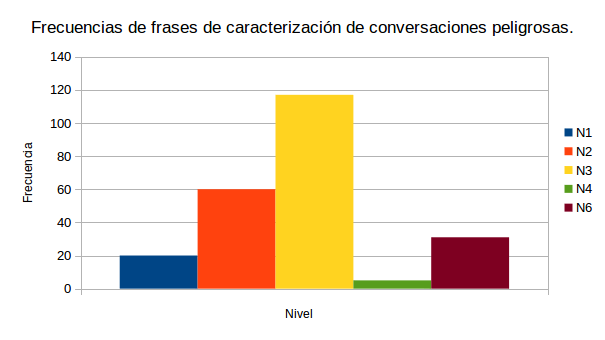
\includegraphics[scale=1]{images/graficanivelespeligrosas}
\caption{Gr\'afica de frecuencias de niveles de conversaciones peligrosas}
\label{fig:graficapeligrosa}
\end{center}
\end{figure}

La gr\'afica \ref{fig:graficanopeligrosa} muestra la estad\'istica de valores de frecuencia obtenidos de la suma de todas las frecuencias de las conversaciones que hemos etiquedo como conversaciones no peligrosas. 

\begin{figure}[h]
\begin{center}
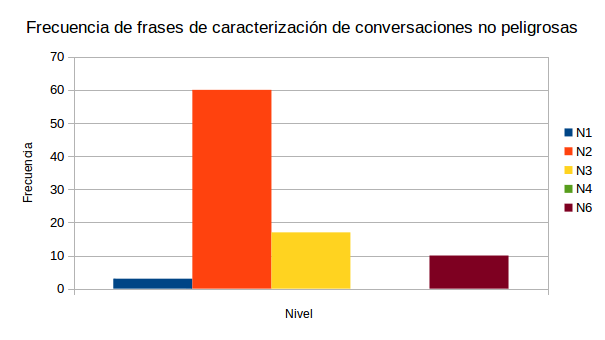
\includegraphics[scale=1]{images/graficanivelesnopeligrosas}
\caption{Gr\'afica de frecuencias de niveles de conversaciones peligrosas}
\label{fig:graficanopeligrosa}
\end{center}
\end{figure}

Haciendo la comparaci\'on de ambas gr\'aficas, se puede observar que  hay presencia de frases de nivel formaci\'on de amistad en ambos tipos de conversaciones, teniendo mayor la frecuencia de este nivel las conversaciones peligrosas.  

En el caso de la formaci\'on de relaci\'on se present\'o un comportamiento donde las conversaciones que marcamos como no peligrosas tienen casi la misma frecuencia que las conversaciones marcadas como peligrosas. Para el caso de frases de nivel de evaluaci\'on de riesgo, donde el objetivo es conocer informaci\'on de los padres, la frecuencia de frases de este nivel es mayor en las de tipo peligrosas, ya que se tiene una frecuencia de 117 a 14 de las no peligrosas. 

El nivel de conclusi\'on se present\'o con una mayor frecuencia en conversaciones peligrosas, esta diferencia es de m\'as del doble comparando un tipo de conversaci\'on con el otro.

Tanto el nivel de reconocimiento del riesgo como de conlusi\'on son niveles donde la diferencia de frecuencias es muy marcada. Pudiendo ser estos niveles aquellos que marcan la diferencia entre un tipo de conversaci\'on y otro. 


\chapter{Prototipo 2:  Generador de Vectores de palabras con denotaci\'on sexual}
\section{Marco Te\'orico}
Tomando en consideraci\'on la matriz de caracterizaci\'on del prototipo anterior. Este prototipo toma como base el Nivel 5 para la extracci\'on de caracter\'isticas pertenecientes a este nivel.

Retomando la tabla \ref{table:caracterizacion} del prototipo anterior, el Nivel 5 contiene una serie de de descriptores de car\'acter sexual. En este nivel el tipo de vocabulario que contienen las conversaciones es meramente relacionado con el contexto sexual.

A diferencia del nivel anterior en este prototipo se trabajar\'a \'unicamente con palabras en lugar de frases, debido a que con base en la observaci\'on el contexto bajo el cual las palabras aparecen es meramente sexual. Decidimos \'unicamente trabajar con la siguiente lista de palabras y sus respectivas derivaciones:

\begin{itemize}
\item Chupar. 
\item Coger. 
\item Follar. 
\item Lamer. 
\item Besar. 
\item Pene. 
\item Vagina. 
\item Masturbar. 
\item Sexo. 
\item Pechos. 
\item Tetas.
\item Clitoris.
\item Tragar.
\end{itemize}


Haciendo una estad\'istica de la frecuencia del stemm de palabras con denotac\'on sexual, se obtuvieron las siguientes gr\'aficas mostradas en las figuras \ref{fig:graficasexual1} y \ref{fig:graficasexual2}. Se puede apreciar que la diferencia de frecuencia de aparici\'on de palabras est\'a muy marcada. Pues en conversaciones no peligrosas la frecuencia es en la mayor\'ia de los casos 0, mientras que en las peligrosas est\'a muy marcada la frecuencia de estas pablabras.

\begin{figure}[h]
\begin{center}
	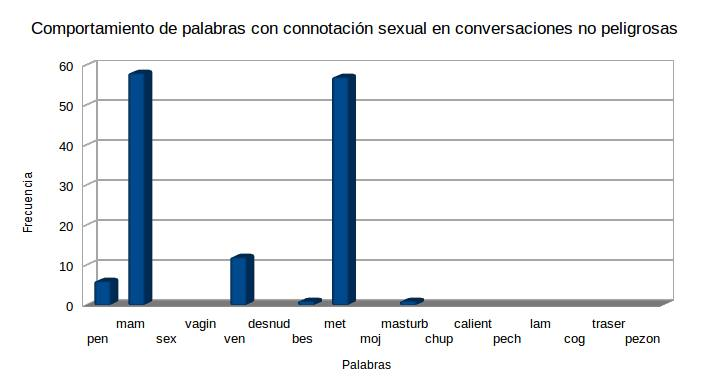
\includegraphics[scale=.6]{images/palabrassexuales1}
	\caption{Frecuencia de palabras de car\'acter sexual en conversaciones no peligrosas}
	\label{fig:graficasexual1}
\end{center}
\end{figure}


\begin{figure}[h]
\begin{center}
	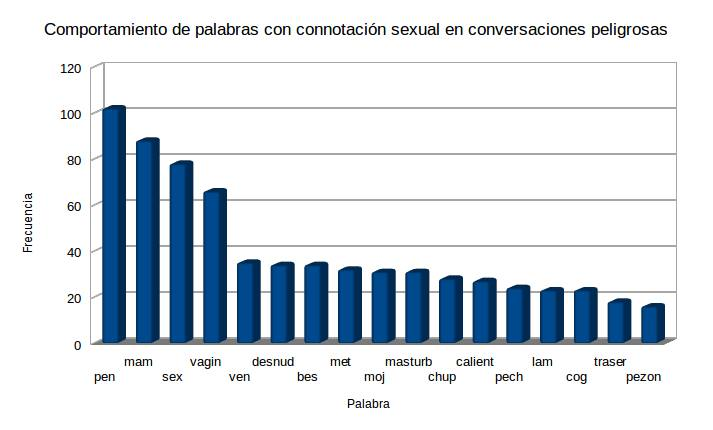
\includegraphics[scale=.6]{images/palabrassexuales2}
	\caption{Frecuencia de palabras de car\'acter sexual en conversaciones peligrosas}
	\label{fig:graficasexual2}
\end{center}
\end{figure}

\section{Descripci\'on}

Este prototipo genera vectores de frecuencia de las palabras del Nivel 5 de la matriz de caracterizaci\'on del comportamiento de conversaciones enfocadas al Online grooming.
\section{Objetivo}
Crear un prototipo que genere vectores de frecuencia de acuerdo al diccionario de palabras correspondientes al Nivel 5 de la matriz de frecuencias de la caracterizaci\'on del comportamiento de conversaciones enfocadas al Online grooming..

\section{An\'alisis}
\subsection{Caracter\'isticas}

\begin{description}
\item[FEAT1] El sistema recibe como entrada una conversaci\'on almacenada en un archivo de texto plano.
\item[FEAT2] El sistema recibe como entrada un archivo una conversaci\'on con un formato xml.
\item[FEAT2] Las palabras del diccionario son editables.
\item[FEAT3] El sistema genera el vector de frecuencias de acuerdo al diccionario dado.
\end{description}

\subsection{Restricciones}
\begin{itemize}
\item Persistencia de vectores en archivos.
\item Lenguaje de programaci\'on python.
\end{itemize}


\section{Dise\~no}

La figura \ref{fig:arquitectura_vector} muestra la arquitectura del comportamiento del prototipo, la cual recibe como entrada las conversaciones en formato plano o con formato xml y como salida se obtiene un vector asociado el cual representa la frecuencia de palabras que pertenecen al Nivel 5 de la matriz de caracterizaci\'on.

\begin{center}
	\begin{figure}[h]
		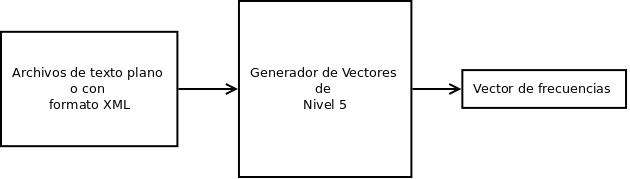
\includegraphics[scale=.5]{images/diagramavectores}
		\caption{Arquitectura Protipo 2}
		\label{fig:arquitectura_vector}
	\end{figure}
\end{center}


En la figura \ref{fig:diagramaActividades} se muestra el diagrama de actividades de la generac\'on de vectores del prototipo. En primer lugar se obtienen las conversaciones de las cuales queremos calcular el vector. El siguiente paso es ignorar palabras sin significado las cuales denominamos stopwords. Obtenemos la ra\'iz mediante el algoritmo de stemming de las palabras. Comparamos las palabras con el diccionario de palabras que tenemos del nivel 5, es decir, las palabras anteriormente listadas. Si la ra\'iz de la palabra que estamos analizando coincide con alguna de nuestro diccionario entonces aumentamos en 1 el valor de la componente del vector que est\'a asociada a dicha palabra.

	\begin{figure}[h]
	\begin{center}
		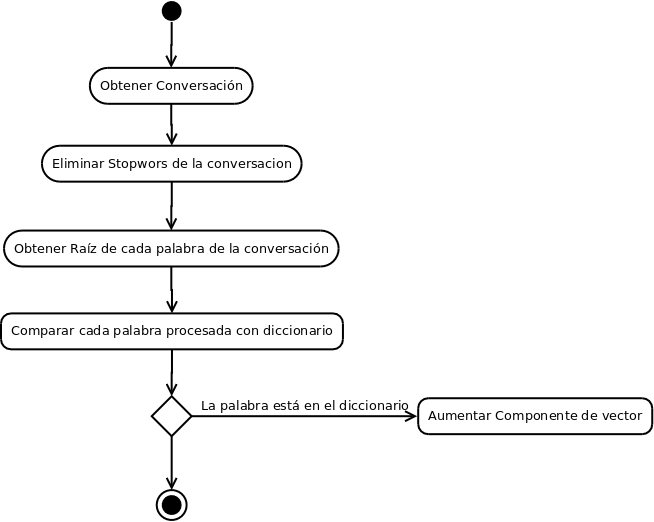
\includegraphics[scale=.35]{images/actividades_vectores}
		\label{fig:diagramaActividades}
		\caption{Diagrama de Actividades del Generador de Vectores}
		\end{center}
	\end{figure}


\section{Resultados}
\subsection{Pruebas}
El prototipo se probó con la generaci\'on de vectores de dimenciones de 3 componentes y 13 componentes.

Las componentes del primer tipo de vector est\'an asociadas al siguiente conjunto de palabras:
\begin{itemize}
\item Lista 1: desnudo, pene, vagina. 

Las componentes del segundo tipo de vector est\'an asociadas al siguiente conjunto de palabras:

\item Lista 2: chupar, coger, follar, lamer, besar, pene, vagina, masturbar, sexo, pechos, tetas, clitoris, tragar.
\end{itemize}

Para ambas listas de palabras se generaron los vectores correspondientes a 50 conversaciones extra\'idas del portal \url{http://www.perverted-justice.com/}, el cual, como ya se hab\'ia mencionado antes, es un sitio donde se hacen p\'ublicas conversaciones que han servido de anzuelo para capturar ped\'ofilos en internet. Estas conversaciones fueron traducidas al español y se anexan en el ap\'endice \ref{app:conversaciones}.


De igual manera se obtuvieron las caracter\'isticas de 50 conversaciones no peligrosas extra\'idas de conversaciones diarias de nuestras cuentas personales de Facebook anexadas en el aprendice \ref{app:conversacionesnp}.

La figura \ref{fig:graficaVectores} muestra la gr\'afica que contiene los vectores de 3 componentes generados por el prototipo. Marcados con puntos amarillos los vectores que representan la clase peligrosa, como podemos observar est\'an en el centro del plano. Mientras que las no peligrosas tienen una disperci\'on fuera del centro. 

Con esto podemos formular una hip\'otesis donde las conversaciones no peligrosas se posicionan en el origen del plano. Con esto podemos decir que este problema es linealmente separable cosa que nos ayudar\'a en la construcci\'on del clasificador. 

\begin{center}
\begin{figure}[h]
	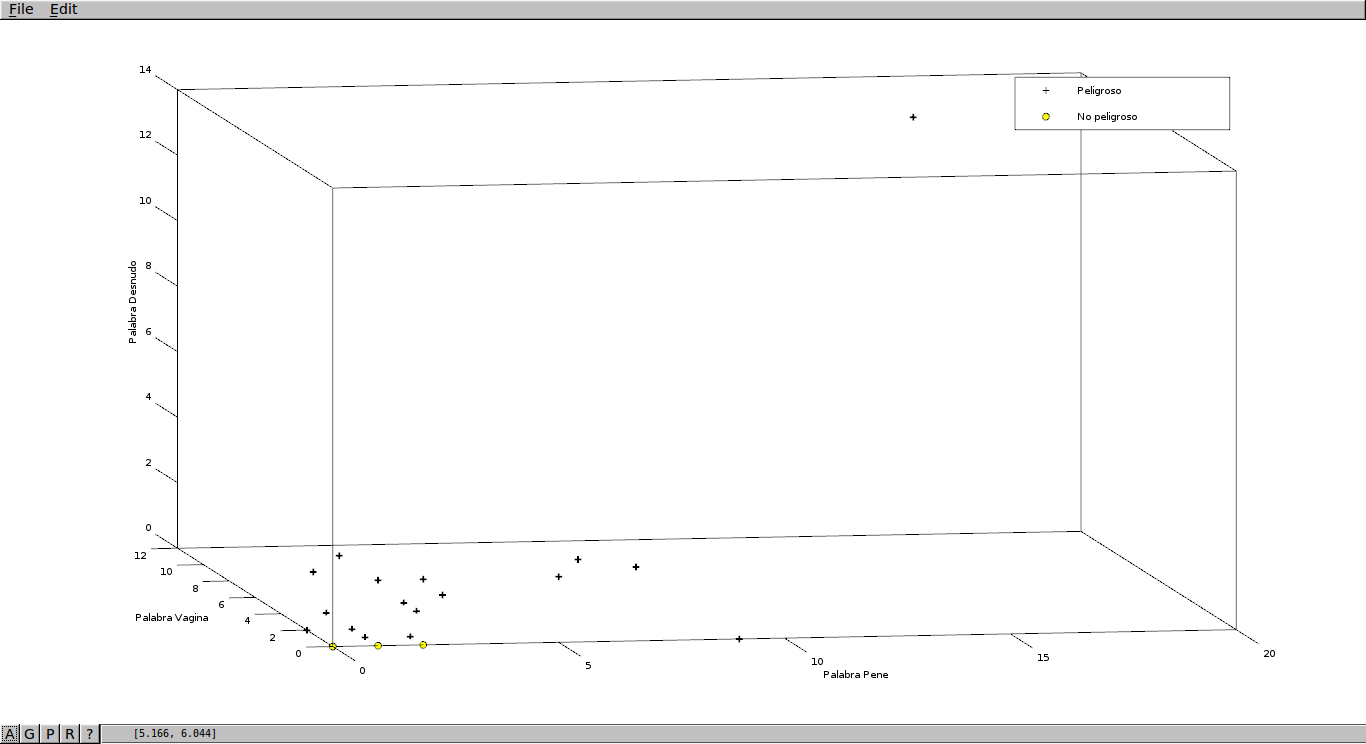
\includegraphics[scale=.3]{images/vectores}
	\caption{Gr\'afica de vectores generados}
	\label{fig:graficaVectores}
\end{figure}
\end{center}

Al aumentar el n\'umero de caracter\'iscas, esperamos que la separabilidad de las clases sea a\'un m\'as evidente por eso hemos seleccionado 13 caracter\'isticas para entrenar al clasificador del prototipo 3.




\chapter{Prototipo 3: Clasificador de conversaciones con denotaci\'on sexual}
\section{An\'alisis}

\subsection{Descripci\'on}

Este prototipo se encarga de la clasificaci\'on de conversaciones en peligrosas o no peligrosas de acuerdo al Nivel 5.

\subsection{Objetivo}
Formular un modelo matem\'atico que permitir\'a la clasificaci\'on de conversaciones peligrosas o no peligrosas de acuerdo al nivel 5 de la matriz de caracterizaci\'on de comportameniento.

\subsection{Caracter\'isticas}
\begin{description}
\item[FEAT1] Plantear el clasificador mediante un modelo matem\'atico usando regresi\'on log\'istica.
\item[FEAT2] Entrenar el clasificador con conversaciones etiquetadas como peligrosas.
\item[FEAT3] Entrenar el clasificador con conversaciones etiquetadas como no peligrosas.
\item[FEAT3] Verificar la eficiencia del clasificador mediante una matriz de confusi\'on.
\end{description}			

\subsection{Restricciones}

\begin{itemize}
\item Clasificador entrenado con aprendizaje supervisado.
\item Implementaci\'on de clasificador en Octave 3.8
\end{itemize}


\subsection{Marco Te\'orico}
\subsubsection{Algoritmo de regresi\'on log\'istica}

El algoritmo de regresi\'on logistica es un m\'etodo estad\'istico que es usado para determinar la ocurrencia de un evento simple valorando diferentes factores.  

Este m\'etodo es adecuado cuando la variable o vector de respuesta $Y$ admite varias categor\'ias de respuesta, es decir, es polit\'omica. Pero es de mayor utilidad cuando \'unicamente nos encontramos con dos posibles respuestas.

Dicho lo anterior, podemos deducir que la variable dependiente $y$ tomar\'a el valor 1 si ocurre el suceso, y por el contrario el valor 0 si no ocurre. La ecuaci\'on \ref{eq:vectory} muestra del conjunto de posibles valores de un clasificador de 2 clases.
\begin{equation}\label{eq:vectory}
y \in {0,1}
\end{equation}

El objetivo de este algortimo es diese\~nar un m\'odelo basado en la formumlaci\'on de una funci\'on $h_{\theta}(x)$ de tal forma que:

\begin{equation}\label{eq:funcionHipotesis}
0 \leq h_{\theta}(x) \leq 1
\end{equation}

La ecuaci\'on \ref{eq:funcionHipotesis} estada dada bajo una relaci\'on de compocici\'on cuyo dominio independiente es el producto matricial del vector de entrada $x$ con un vector de param\'etros $\theta$. La ecucio\'on \ref{eq:composicion}

\begin{equation}\label{eq:composicion}
h_{\theta}(x) = g(\theta x)
\end{equation}

La funci\'on $g(z)$ est\'a descrita en relaci\'on a la funci\'on sigmoide descrita en la ecuaci\'on \ref{eq:sigmoide} la cual es utilizada como curva de aprendizaje de sistemas complejos.


\begin{equation}\label{eq:sigmoide}
g(z) = \frac{1}{1+e^z}
\end{equation}
donde:
\begin{equation}
z = \theta_{0}x_{0}+ \theta_{1}x_{1} + ... +  \theta_{n}x_{n}
\end{equation}

La figura \ref{fig:sigmoide} muestra la gr\'afica de la funci\'on sigmoide cuyo comportamiento est\'a dado por las ecuaciones \ref{eq:limite1} y \ref{eq:limite2}

\begin{equation}\label{eq:limite1}
\lim_{z \to \infty} g(z) = 1
\end{equation}

\begin{equation}\label{eq:limite2}
\lim_{z \to -\infty} g(z) = 1
\end{equation}
donde:
\begin{equation}
z = \theta_{0}x_{0}+ \theta_{1}x_{1} + ... +  \theta_{n}x_{n}
\end{equation}

\begin{figure}[h]
	\begin{center}
		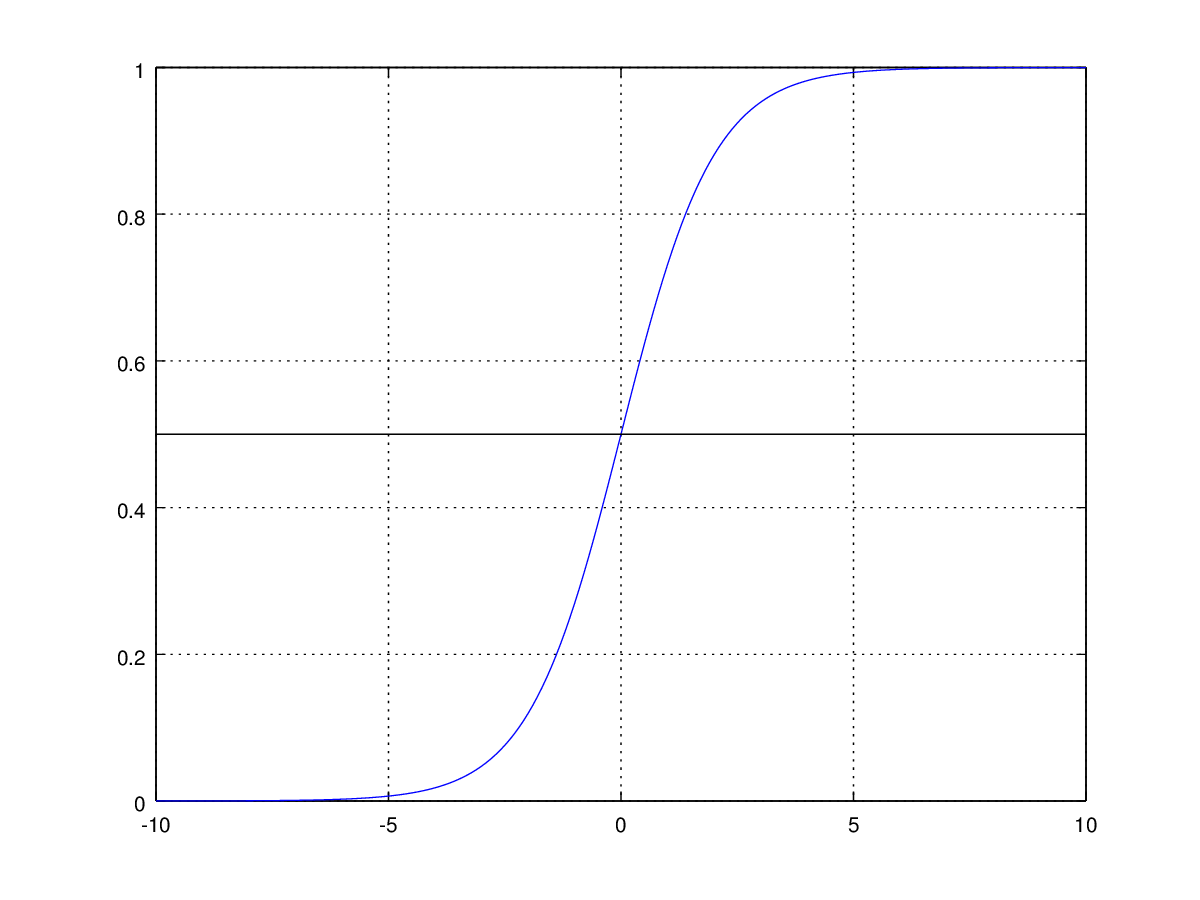
\includegraphics[scale=.5]{images/sigmoide}
		\caption{Gr\'afica de la funci\'on sigmoide}
		\label{fig:sigmoide}
	\end{center}
\end{figure}

La manera en que se interpreta el resultado de la funci\'on sinoide es la siguiente.

Sea $x$ un vector donde cada componente indica una caracter\'istica en particular:

\begin{equation}
x  = 
\begin{bmatrix}
x_{0} \\
x_{1} \\
\vdots \\
x_{n}
\end{bmatrix}
\end{equation}

Entonces si $h_{\theta}(x) = 0.7$ decimos que hay un 70\% de probabilidad de que el vector $x$ pertenezca a la clase etiquetada con valor 1.

Dentro de este algoritmo podemos definir una frontera de desici\'on la cual indique el umbral de valores para que un vector pertenezca a una clase u otra.

Por ejemplo $y = 1$ si se cumple la condici\'on: 
\begin{equation}
h_{\theta}(x) \geq 0.5
\end{equation}
De lo contrario $y = 0$ si
\begin{equation}
h_{\theta}(x) < 0.5
\end{equation}

El objetivo del algoritmo es encontrar el vector $\theta$ \'optimo de tal manera de formular un m\'odelo lineal que separe las clases como el ejemplo de la figura \ref{fig:ejemploClases}

\begin{figure}[h!]
	\begin{center}
	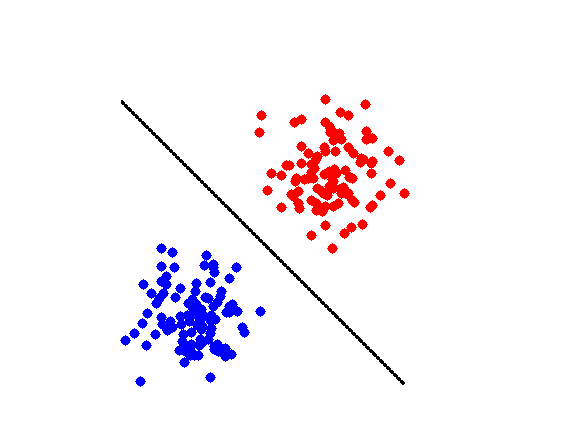
\includegraphics[scale=.3]{images/clasesejemplo}
	\caption{Ejemplo de separaci\'on de Clases}
	\label{fig:ejemploClases}
	\end{center}
\end{figure}

Para evaluar el costo de los parametros del vector $\theta$ se tiene la siguiente ecuaci\'on:
\begin{equation}
costo(h_{\theta}(x),y) = -yln(h_{\theta}(x))-(1-y)ln(1-h_{\theta}(x))
\end{equation}

\section{Dise\~no}
\subsection{Arquitectura}
La figura \ref{fig:arquitecturaClasificador} muestra la arquitectura del prototipo de clasificaci\'on del Nivel 5.
\begin{figure}[h]
	\begin{center}
	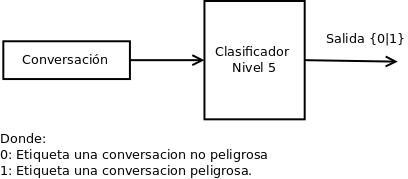
\includegraphics[scale=.5]{images/arquitecturaClasificador}
	\caption{Ejemplo de separaci\'on de Clases}
	\label{fig:arquitecturaClasificador}
	\end{center}
\end{figure}

\section{Pruebas}

\subsection{Entrenamiento con 3 variables}
Se realiz\'o el entrenamiento con 3 variables las cuales corresponden a las componentes del vector generado por el prototipo 1 con la siguiente lista de palabras:
\begin{itemize}
\item Pene
\item Vagina
\item Desnudo
\end{itemize}

Estas variables generaron un vector $\theta$ con los siguientes valores:

\begin{equation}
\theta = 
\begin{bmatrix}

-0.613684 \\
 0.904610 \\
 1.221655 \\
 0.726040
\end{bmatrix}
\end{equation}

La tabla \ref{tab:confucion1} muestra la tabla de confusi\'on de este entrenamiento.


\begin{table}[h]
\begin{center}
\begin{tabular}{c|c|c|c|c|}
\multicolumn{5}{c}{Predicci\'on} \\
\cline{2-5}
& & Conversaci\'on No Peligrosas & Conversaci\'on Peligrosas &  Presici\'on \\
\cline{2-5}
\multirow{2}{*}{Actual} & Conversaci\'on no Peligrosa & 17 & 3 & 85\% \\
\cline{2-5}
& Conversaci\'on Peligrosa &  6 & 33 & 84\% \\
\cline{2-5}

\end{tabular}
\caption{Tabla de Confuci\'on con 3 rasgos}
\label{tab:confucion1}
\end{center}
\end{table}

Con esto se tiene una precisi\'on de un 84.5\% del clasificador.
La figura \ref{fig:separabilidad} muestra de manera gr\'afica un plano que muestra la separabilidad de las clases con vectores de 3 componentes.

\begin{figure}
	\begin{center}
	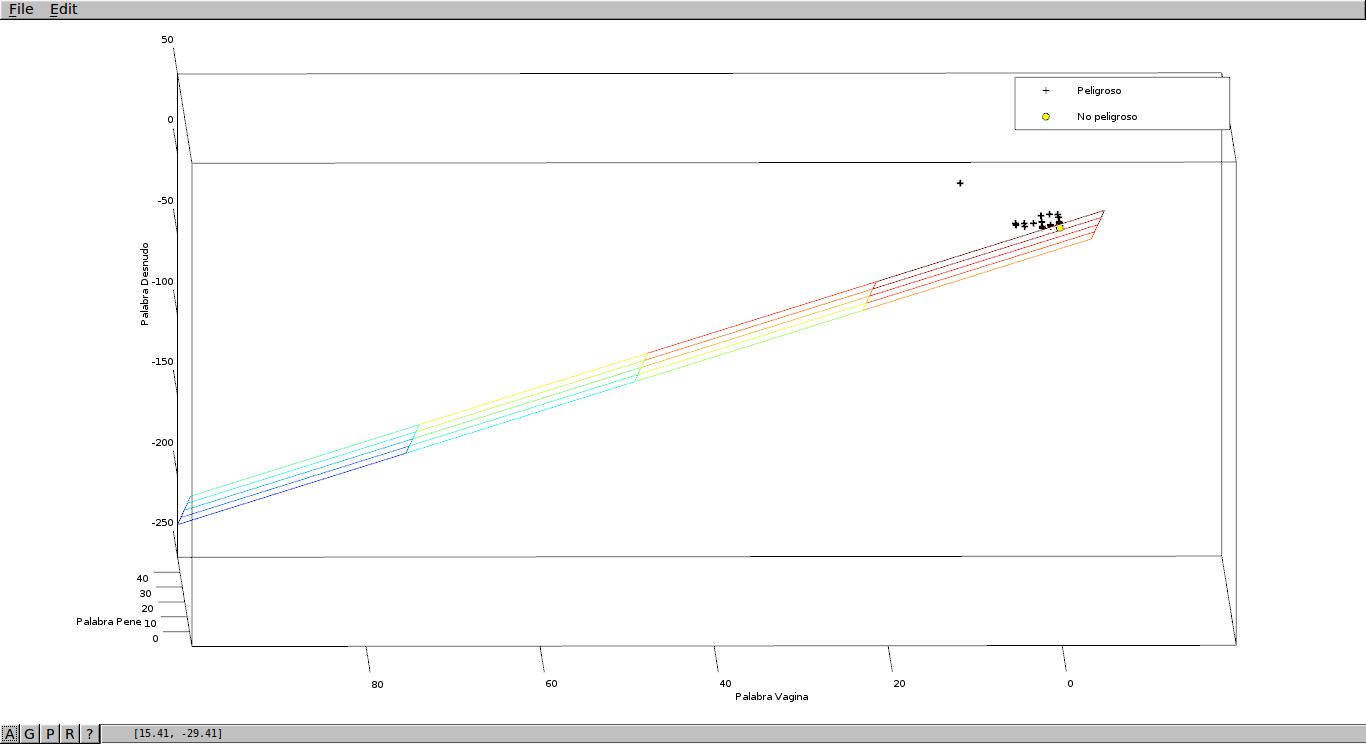
\includegraphics[scale=.4]{images/separavilidad}
	\caption{Gr\'afica que muestra la separabilidad del clasificador.}
	\label{fig:separabilidad}
	\end{center}
\end{figure}


\subsection{Entrenamiento con 14 variables}
Se realiz\'o el entrenamiento con 3 variables las cuales corresponden a las componentes del vector generado por el prototipo 1 con la siguiente lista de palabras:
\begin{itemize}
\item chupar 
\item coger
\item follar
\item lamer
\item besar
\item pene 
\item vagina
\item masturbar
\item sexo
\item pechos
\item tetas
\item clitoris
\item tragar
\item violar
\end{itemize}

Estas variables generaron un vector $\theta$ con los siguientes valores:

\begin{equation}
\theta = 
\begin{bmatrix}

-1.027760 \\
 0.704011 \\
 0.907893 \\
 0.588279 \\
 0.529208 \\
 0.203309 \\
 0.104863 \\
 1.167757 \\
 0.975621 \\
 0.348992 \\
 0.541306 \\
 0.622848 \\
 0.233392 \\
 0.039713 \\
 -0.066605
 
\end{bmatrix}
\end{equation}

La tabla \ref{tab:confucion2} muestra la tabla de confusi\'on de este entrenamiento.


\begin{table}[h]
\begin{center}
\begin{tabular}{c|c|c|c|c|}
\multicolumn{5}{c}{Predicci\'on} \\
\cline{2-5}
& & Conversaci\'on No Peligrosas & Conversaci\'on Peligrosas &  Presici\'on \\
\cline{2-5}
\multirow{2}{*}{Actual} & Conversaci\'on no Peligrosa & 20 & 0 & 100\% \\
\cline{2-5}
& Conversaci\'on Peligrosa &  2 & 41 & 95\% \\
\cline{2-5}

\end{tabular}
\caption{Tabla de Confusi\'on con 3 rasgos}
\label{tab:confucion2}
\end{center}
\end{table}

Con esto se tiene una precisi\'on de un 96.72\% del clasificador.


Para el valor de prediction tenemos 

%\begin{equation}
%\frac{TruePositives}{TruePositiveP + FalseNegatives)

\begin{equation}\label{eq:sigmoide}
\frac{TruePositives}{TruePositive + FalsePositives} = \frac{41}{41+2} = 0.9534
\end{equation} 

El valor del recall es: 

\begin{equation}\label{eq:sigmoide}
\frac{TruePositives}{TruePositive + FalseNegatives} = \frac{41}{41+2
0} = 1
\end{equation}

Ambos valores nos indican que esa cantidad de desciriptores del clasificador lo hacen tener un buen desempe\~no.




\chapter{Prototipo 4: Clasfificador de comportamiento de conversaciones}

\section{An\'alisis}
Este prototipo determina una clasificaci\'on de las conversaciones en 4 niveles de peligrosidad: No peligrosa, Poco peligrosa, Peligrosa y Muy peligrosa. 

\subsection{Objetivo}
Ralizar un m\'odulo que sea capaz de determinar el nivel de peligrosidad de una conversaci\'on en las siguientes clases: No peligrosa, Poco peligrosa, Peligrosa y Muy peligrosa. 

\subsection{Caracter\'isticas}
\begin{description}
\item[FEAT1:] El sistema analiza el vector generado en el prototipo 2.
\item[FEAT2:] El sistema toma como entrada la clase resultante del prototipo 3.
\item[FEAT3:] Se plantea un modelo mediante una red neuronal para la clasificaci\'on.

\end{description}

\subsection{Restricciones}

\begin{itemize}
\item  Uso de t\'ecnicas de l\'ogica difusa.
\item  Prototipo programado en Octave versi\'on 3.8.
\end{itemize}

\subsection{Marco Te\'orico}
\subsubsection{Red Neuronal}
Las redes neuronales son sistemas ideados como abstracciones de las estructuras neurobiol\'ogicas encontradas en la naturaleza y tienen la caracter\'istica de ser sistemas desordenados capaces de guardar informaci\'on.

La forma en que desarrollan su trabajo es esencialmente distinta de la utilizada por las computadoras convencionales. Los procesadores microsc\'opicos del cerebro (neuronas) operan en paralelo y presentan cualitativamente m\'as ruido que los elementos que forman a las computadoras. No ejecutan un programa fijo con base en un conjunto previamente especificado de datos, sino que comunican se\~nales a trav\'es de retransmisores que llamamos sin\'apsis, que llegan a centros de conjunci\'on llamados los cuerpos de las neuronas y desde los cuales surgen señales el\'ectricas a trav\'es de canales conocidos con el nombre de axones.

La importancia de cada sin\'apsis en el proceso de retransmisi\'on se actualiza continuamente y lo mismo ocurre con algunas propiedades intr\'insecas de las neuronas, proporcionando un sistema de autoprogramaci\'on y adaptaci\'on que sustituye a la programaci\'on externa de los sistemas de c\'omputo comunes. Existe as\'i una din\'amica de las sin\'apsis y de las neuronas en el cual los programas y los datos cambian todo el tiempo.

\subsubsection{BackPropagation}

La propagaci\'on hacia atr\'as de errores o retropropagaci\'on (del ingl\'es backpropagation) es un algoritmo de aprendizaje supervisado que se usa para entrenar redes neuronales artificiales. El algoritmo emplea un ciclo propagaci\'on – adaptaci\'on de dos fases. Una vez que se ha aplicado un patr\'on a la entrada de la red como est\'imulo, este se propaga desde la primera capa a trav\'es de las capas superiores de la red, hasta generar una salida. 

\subsubsection{L\'ogica difusa}
La l\'ogica difusa es una extensi\'on de la l\'ogica tradicional(Booleana) que utiliza conceptos de pertenencia de sistemas parecidos a la manera de pensar humana.

A partir de la  observaci\'on del nivel 3 de la matriz de caracterizaci\'on se hace notar, este nivel, como discriminante para diferenciar una conversaci\'on peligrosa de otra no peligrosa a partir de la media. Se obtuvo una media 3 incidencias de ese nivel en conversaciones peligrosas. De acuerdo a esto se dedujo la tabla \ref{tab:TablaNiveles}.



\begin{longtable}{|c|c|c|c|c|c|c|c|c|c|c|}

\hline
N1 & N2 & N3 & N3\_2 & N4 & N5 & N6 & No Peligrosa & Poco Peligrosa & Peligrosa & Muy Peligrosa \\
\hline
\endfirsthead


\hline
N1 & N2 & N3 & N3\_2 &  N4 & N5 & N6 & No Peligrosa & Poco Peligrosa & Peligrosa & Muy Peligrosa \\
\hline
\endhead
\hline
\multicolumn{11}{c}{Sigue en la p\'agina siguiente.}
\endfoot
\endlastfoot


0 & 0 & 0 & 0 & 0 & 0 & 0 &  1 & 0 & 0 & 0 \\
0 & 0 & 0 & 0 & 0 & 0 & 1 &  0 & 1 & 0 & 0 \\
0 & 0 & 0 & 0 & 0 & 1 & 0 &  0 & 0 & 0 & 1 \\
0 & 0 & 0 & 0 & 0 & 1 & 1 &  0 & 0 & 0 & 1 \\
0 & 0 & 0 & 0 & 1 & 0 & 0 &  0 & 0 & 1 & 0 \\
0 & 0 & 0 & 0 & 1 & 0 & 1 &  0 & 0 & 1 & 0 \\
0 & 0 & 0 & 0 & 1 & 1 & 0 &  0 & 0 & 0 & 1 \\
0 & 0 & 0 & 0 & 1 & 1 & 1 &  0 & 0 & 0 & 1 \\
0 & 0 & 0 & 1 & 0 & 0 & 0 &  0 & 1 & 0 & 0 \\
0 & 0 & 0 & 1 & 0 & 0 & 1 &  0 & 0 & 1 & 0 \\
0 & 0 & 0 & 1 & 0 & 1 & 0 &  0 & 0 & 0 & 1 \\
0 & 0 & 0 & 1 & 0 & 1 & 1 &  0 & 0 & 0 & 1 \\
0 & 0 & 0 & 1 & 1 & 0 & 0 &  0 & 0 & 1 & 0 \\
0 & 0 & 0 & 1 & 1 & 0 & 1 &  0 & 0 & 1 & 0 \\
0 & 0 & 0 & 1 & 1 & 1 & 0 &  0 & 0 & 0 & 1 \\
0 & 0 & 0 & 1 & 1 & 1 & 1 &  0 & 0 & 0 & 1 \\
0 & 0 & 1 & 0 & 0 & 0 & 0 &  1 & 0 & 0 & 0 \\
0 & 0 & 1 & 0 & 0 & 0 & 1 &  0 & 1 & 0 & 0 \\
0 & 0 & 1 & 0 & 0 & 1 & 0 &  0 & 0 & 0 & 1 \\
0 & 0 & 1 & 0 & 0 & 1 & 1 &  0 & 0 & 0 & 1 \\
0 & 0 & 1 & 0 & 1 & 0 & 0 &  0 & 1 & 0 & 0 \\
0 & 0 & 1 & 0 & 1 & 0 & 1 &  0 & 1 & 0 & 0 \\
0 & 0 & 1 & 0 & 1 & 1 & 0 &  0 & 0 & 0 & 1 \\
0 & 0 & 1 & 0 & 1 & 1 & 1 &  0 & 0 & 0 & 1 \\
0 & 0 & 1 & 1 & 0 & 0 & 0 &  0 & 1 & 0 & 0 \\
0 & 0 & 1 & 1 & 0 & 0 & 1 &  0 & 0 & 1 & 0 \\
0 & 0 & 1 & 1 & 0 & 1 & 0 &  0 & 0 & 0 & 1 \\
0 & 0 & 1 & 1 & 0 & 1 & 1 &  0 & 0 & 0 & 1 \\
0 & 0 & 1 & 1 & 1 & 0 & 0 &  0 & 0 & 1 & 0 \\
0 & 0 & 1 & 1 & 1 & 0 & 1 &  0 & 0 & 1 & 0redneuronal \\
0 & 0 & 1 & 1 & 1 & 1 & 0 &  0 & 0 & 0 & 1 \\
0 & 0 & 1 & 1 & 1 & 1 & 1 &  0 & 0 & 0 & 1 \\
0 & 1 & 0 & 0 & 0 & 0 & 0 &  1 & 0 & 0 & 0 \\
0 & 1 & 0 & 0 & 0 & 0 & 1 &  0 & 1 & 0 & 0 \\
0 & 1 & 0 & 0 & 0 & 1 & 0 &  0 & 0 & 0 & 1 \\
0 & 1 & 0 & 0 & 0 & 1 & 1 &  0 & 0 & 0 & 1 \\
0 & 1 & 0 & 0 & 1 & 0 & 0 &  0 & 1 & 0 & 0 \\
0 & 1 & 0 & 0 & 1 & 0 & 1 &  0 & 1 & 0 & 0 \\
0 & 1 & 0 & 0 & 1 & 1 & 0 &  0 & 0 & 0 & 1 \\
0 & 1 & 0 & 0 & 1 & 1 & 1 &  0 & 0 & 0 & 1 \\
0 & 1 & 0 & 1 & 0 & 0 & 0 &  0 & 1 & 0 & 0 \\
0 & 1 & 0 & 1 & 0 & 0 & 1 &  0 & 1 & 0 & 0 \\
0 & 1 & 0 & 1 & 0 & 1 & 0 &  0 & 0 & 0 & 1 \\
0 & 1 & 0 & 1 & 0 & 1 & 1 &  0 & 0 & 0 & 1 \\
0 & 1 & 0 & 1 & 1 & 0 & 0 &  0 & 1 & 0 & 0 \\
0 & 1 & 0 & 1 & 1 & 0 & 1 &  0 & 0 & 1 & 0 \\
0 & 1 & 0 & 1 & 1 & 1 & 0 &  0 & 0 & 0 & 1 \\
0 & 1 & 0 & 1 & 1 & 1 & 1 &  0 & 0 & 0 & 1 \\
0 & 1 & 1 & 0 & 0 & 0 & 0 &  1 & 0 & 0 & 0 \\
0 & 1 & 1 & 0 & 0 & 0 & 1 &  1 & 0 & 0 & 0 \\
0 & 1 & 1 & 0 & 0 & 1 & 0 &  0 & 0 & 0 & 1 \\
0 & 1 & 1 & 0 & 0 & 1 & 1 &  0 & 0 & 0 & 1 \\
0 & 1 & 1 & 0 & 1 & 0 & 0 &  0 & 1 & 0 & 0 \\
0 & 1 & 1 & 0 & 1 & 0 & 1 &  0 & 1 & 0 & 0 \\
0 & 1 & 1 & 0 & 1 & 1 & 0 &  0 & 0 & 0 & 1 \\
0 & 1 & 1 & 0 & 1 & 1 & 1 &  0 & 0 & 0 & 1 \\
0 & 1 & 1 & 1 & 0 & 0 & 0 &  0 & 1 & 0 & 0 \\
0 & 1 & 1 & 1 & 0 & 0 & 1 &  0 & 1 & 0 & 0 \\
0 & 1 & 1 & 1 & 0 & 1 & 0 &  0 & 0 & 0 & 1 \\
0 & 1 & 1 & 1 & 0 & 1 & 1 &  0 & 0 & 0 & 1 \\
0 & 1 & 1 & 1 & 1 & 0 & 0 &  0 & 0 & 1 & 0 \\
0 & 1 & 1 & 1 & 1 & 0 & 1 &  0 & 0 & 1 & 0 \\
0 & 1 & 1 & 1 & 1 & 1 & 0 &  0 & 0 & 0 & 1 \\
0 & 1 & 1 & 1 & 1 & 1 & 1 &  0 & 0 & 0 & 1 \\
1 & 0 & 0 & 0 & 0 & 0 & 0 &  1 & 0 & 0 & 0 \\
1 & 0 & 0 & 0 & 0 & 0 & 1 &  1 & 0 & 0 & 0 \\
1 & 0 & 0 & 0 & 0 & 1 & 0 &  0 & 0 & 0 & 1 \\
1 & 0 & 0 & 0 & 0 & 1 & 1 &  0 & 0 & 0 & 1 \\
1 & 0 & 0 & 0 & 1 & 0 & 0 &  0 & 1 & 0 & 0 \\
1 & 0 & 0 & 0 & 1 & 0 & 1 &  0 & 0 & 1 & 0 \\
1 & 0 & 0 & 0 & 1 & 1 & 0 &  0 & 0 & 0 & 1 \\
1 & 0 & 0 & 0 & 1 & 1 & 1 &  0 & 0 & 0 & 1 \\
1 & 0 & 0 & 1 & 0 & 0 & 0 &  0 & 1 & 0 & 0 \\
1 & 0 & 0 & 1 & 0 & 0 & 1 &  0 & 0 & 1 & 0 \\
1 & 0 & 0 & 1 & 0 & 1 & 0 &  0 & 0 & 0 & 1 \\
1 & 0 & 0 & 1 & 0 & 1 & 1 &  0 & 0 & 0 & 1 \\
1 & 0 & 0 & 1 & 1 & 0 & 0 &  0 & 0 & 1 & 0 \\
1 & 0 & 0 & 1 & 1 & 0 & 1 &  0 & 0 & 1 & 0 \\
1 & 0 & 0 & 1 & 1 & 1 & 0 &  0 & 0 & 0 & 1 \\
1 & 0 & 0 & 1 & 1 & 1 & 1 &  0 & 0 & 0 & 1 \\
1 & 0 & 1 & 0 & 0 & 0 & 0 &  1 & 0 & 0 & 0 \\
1 & 0 & 1 & 0 & 0 & 0 & 1 &  1 & 0 & 0 & 0 \\
1 & 0 & 1 & 0 & 0 & 1 & 0 &  0 & 0 & 0 & 1 \\
1 & 0 & 1 & 0 & 0 & 1 & 1 &  0 & 0 & 0 & 1 \\
1 & 0 & 1 & 0 & 1 & 0 & 0 &  0 & 1 & 0 & 0 \\
1 & 0 & 1 & 0 & 1 & 0 & 1 &  0 & 1 & 0 & 0 \\
1 & 0 & 1 & 0 & 1 & 1 & 0 &  0 & 0 & 0 & 1 \\
1 & 0 & 1 & 0 & 1 & 1 & 1 &  0 & 0 & 0 & 1 \\
1 & 0 & 1 & 1 & 0 & 0 & 0 &  0 & 1 & 0 & 0 \\
1 & 0 & 1 & 1 & 0 & 0 & 1 &  0 & 1 & 0 & 0 \\
1 & 0 & 1 & 1 & 0 & 1 & 0 &  0 & 0 & 0 & 1 \\
1 & 0 & 1 & 1 & 0 & 1 & 1 &  0 & 0 & 0 & 1 \\
1 & 0 & 1 & 1 & 1 & 0 & 0 &  0 & 0 & 1 & 0 \\
1 & 0 & 1 & 1 & 1 & 0 & 1 &  0 & 0 & 1 & 0 \\
1 & 0 & 1 & 1 & 1 & 1 & 0 &  0 & 0 & 0 & 1 \\
1 & 0 & 1 & 1 & 1 & 1 & 1 &  0 & 0 & 0 & 1 \\
1 & 1 & 0 & 0 & 0 & 0 & 0 &  1 & 0 & 0 & 0 \\
1 & 1 & 0 & 0 & 0 & 0 & 1 &  1 & 0 & 0 & 0 \\
1 & 1 & 0 & 0 & 0 & 1 & 0 &  0 & 0 & 0 & 1 \\
1 & 1 & 0 & 0 & 0 & 1 & 1 &  0 & 0 & 0 & 1 \\
1 & 1 & 0 & 0 & 1 & 0 & 0 &  0 & 1 & 0 & 0 \\
1 & 1 & 0 & 0 & 1 & 0 & 1 &  0 & 0 & 1 & 0 \\
1 & 1 & 0 & 0 & 1 & 1 & 0 &  0 & 0 & 0 & 1 \\
1 & 1 & 0 & 0 & 1 & 1 & 1 &  0 & 0 & 0 & 1 \\
1 & 1 & 0 & 1 & 0 & 0 & 0 &  0 & 1 & 0 & 0 \\
1 & 1 & 0 & 1 & 0 & 0 & 1 &  0 & 0 & 1 & 0 \\
1 & 1 & 0 & 1 & 0 & 1 & 0 &  0 & 0 & 0 & 1 \\
1 & 1 & 0 & 1 & 0 & 1 & 1 &  0 & 0 & 0 & 1 \\
1 & 1 & 0 & 1 & 1 & 0 & 0 &  0 & 0 & 1 & 0 \\
1 & 1 & 0 & 1 & 1 & 0 & 1 &  0 & 0 & 1 & 0 \\
1 & 1 & 0 & 1 & 1 & 1 & 0 &  0 & 0 & 0 & 1 \\
1 & 1 & 0 & 1 & 1 & 1 & 1 &  0 & 0 & 0 & 1 \\
1 & 1 & 1 & 0 & 0 & 0 & 0 &  1 & 0 & 0 & 0 \\
1 & 1 & 1 & 0 & 0 & 0 & 1 &  1 & 0 & 0 & 0 \\
1 & 1 & 1 & 0 & 0 & 1 & 0 &  0 & 0 & 0 & 1 \\
1 & 1 & 1 & 0 & 0 & 1 & 1 &  0 & 0 & 0 & 1 \\
1 & 1 & 1 & 0 & 1 & 0 & 0 &  0 & 1 & 0 & 0 \\
1 & 1 & 1 & 0 & 1 & 0 & 1 &  0 & 0 & 1 & 0 \\
1 & 1 & 1 & 0 & 1 & 1 & 0 &  0 & 0 & 0 & 1 \\
1 & 1 & 1 & 0 & 1 & 1 & 1 &  0 & 0 & 0 & 1 \\
1 & 1 & 1 & 1 & 0 & 0 & 0 &  0 & 1 & 0 & 0 \\
1 & 1 & 1 & 1 & 0 & 0 & 1 &  0 & 0 & 1 & 0 \\
1 & 1 & 1 & 1 & 0 & 1 & 0 &  0 & 0 & 0 & 1 \\
1 & 1 & 1 & 1 & 0 & 1 & 1 &  0 & 0 & 0 & 1 \\
1 & 1 & 1 & 1 & 1 & 0 & 0 &  0 & 0 & 1 & 0 \\
1 & 1 & 1 & 1 & 1 & 0 & 1 &  0 & 0 & 0 & 0 \\
1 & 1 & 1 & 1 & 1 & 1 & 0 &  0 & 0 & 0 & 1 \\ 
1 & 1 & 1 & 1 & 1 & 1 & 1 &  0 & 0 & 0 & 1 \\
\hline

\caption{Clasificador de Niveles}
\label{tab:TablaNiveles}
\end{longtable}

\section{Dise\~no}
La figura \ref{fig:arquitecturaNivel4} muestra la arquitectura del prototipo donde las flechas de salida indican la decisi\'on que el clasificador toma. Si la salida es 0001 indica que la conversaci\'on no es peligrosa. Si la salida es 0010 indica que la conversaci\'ion es poco peligrosa. Si la salida es 0100 indica que la conversaci\'ion es peligrosa. Si la salida es 1000 indica que la conversaci\'ion no es muy peligrosa.

\begin{figure}
\begin{center}
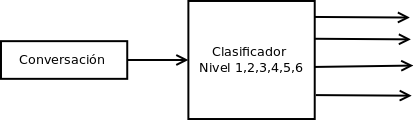
\includegraphics[scale=.5]{images/arquitecturaprotipo4}
\caption{Arquitectura prototipo 4}
\label{fig:arquitecturaNivel4}
\end{center}
\end{figure} 

\subsection{Dise\~no de la red neuronal}
La arquitectura que tendr\'a la red neuronal est\'a presentado en la figura \ref{fig:redNeuronal} donde la capa de entrada represantan los vectores de los niveles descritos anteriormente, la capa oculta est\'a constituida por 7 neuronas y la capa de salida por 4.

\begin{figure}
\begin{center}
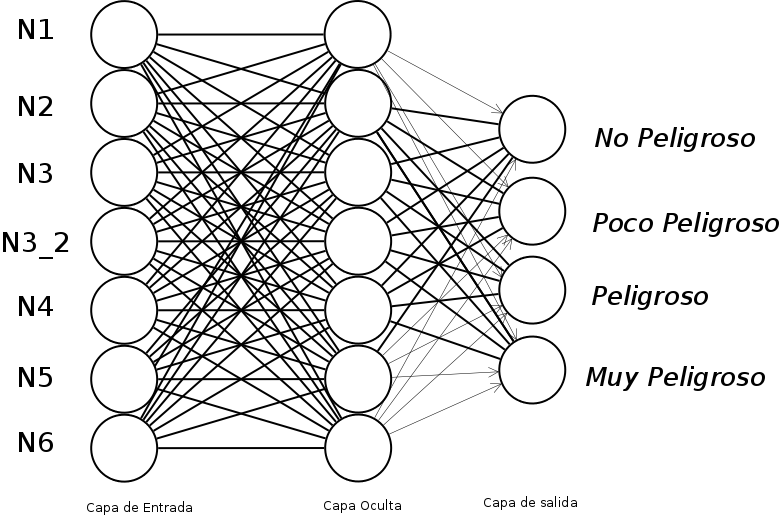
\includegraphics[scale=.5]{images/redneuronal}
\caption{Arquitectura de la Red Neuronal del prototipo 4}
\label{fig:redNeuronal}
\end{center}
\end{figure}

Dicha red fue entrenada con el algorimo de aprendizaje Backpropagation.

\section{Pruebas} 

La figurura \ref{fig:mconfucion} muestra la matriz de confusi\'on donde se muestra una precisi\'on del 98.9\%.

\begin{figure}[h]
\begin{center}
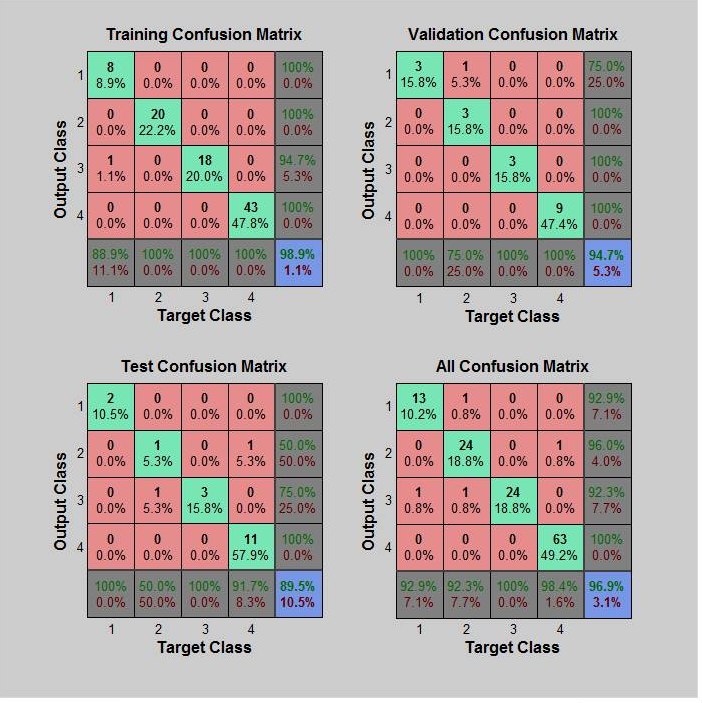
\includegraphics[scale=.5]{images/mcofucion}
\caption{Matriz de confusi\'on del clasificador}
\label{fig:mconfucion}
\end{center}
\end{figure}



\chapter{Prototipo 5: API de desici\'on}
\section{An\'alisis}

\subsection{Descripci\'on}
Este prototipo se encarga de la toma de desiciones del clasificador de nivel 5 y el clasificador de niveles  1, 2, 3, 4 y 6.

\subsection{Objetivo}
Desarrollar el API de desici\'on a partir de la uni\'on de los clasificadores de nivel 5 y niveles 1, 2, 3, 4 y 6.

\subsection{Caracter\'isticas}
\begin{description}
\item[FEAT1:] La API recibe como entrada conversaciones en archivos de texto plano.
\item[FEAT2:] La API recibe como entrada conversaciones en archivos con formato xml.
\item[FEAT4:] La API preprocesa textos.
\item[FEAT4:] La API genera vectores de nivel 5.
\item[FEAT5:] La API genera vectores de nivel  1, 2, 3, 4 y 6.
\item[FEAT6:] El API dar\'a como salida la desici\'on del clasificador dle prototipo4.

\end{description}

\section{Dise\~no}


\section{Arquitectura}

La figura \ref{fig:arquitecturap5} muestra la arquitectura de la API de an\'alisis.

\begin{figure}[h]
\begin{center}
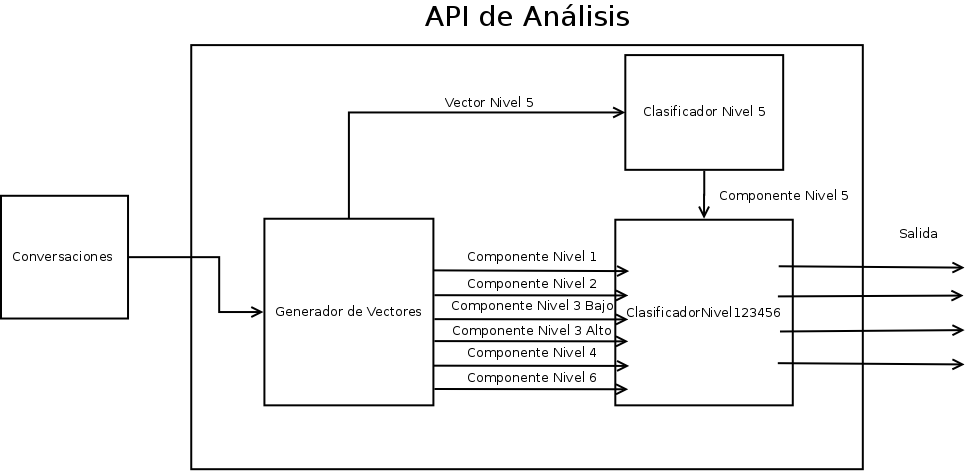
\includegraphics[scale=.3]{images/api}
\caption{Arquitectura de la API de ana\'alisis}
\label{fig:arquitecturap5}
\end{center}
\end{figure}


\subsection{Diagrama de clases}


La figura \ref{fig:dclasesp5} muestra el diagrama de clases de la API de an\'alisis.
\begin{figure}[h]
\begin{center}
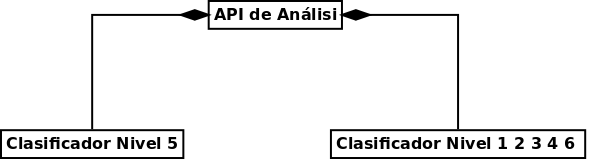
\includegraphics[scale=.5]{images/clasesnivel5}
\caption{Diagrama de clases de la API de ana\'alisis}
\label{fig:dclasesp5}
\end{center}
\end{figure}

\section{Pruebas}


La tabla  \ref{tab:resultadasapi} muestra la tabla de resultados de conversaciones nuevas y su respectivo resultado.

\begin{table}
\begin{center}


\begin{tabular}{|l|c|c|c|c|c|c|c|c|}

\hline
Conversaci\'on & N1 & N2 & N3 & N\_3 & N4 & N5 & N6 & Decisi\'on \\
\hline
pruebas/pr10.txt &
 0 &
 3 &
 0 &
 0 &
 0 &
 1 &
 1 &
Muy Peligrosa \\
pruebas/pr11.txt &
 0 &
 4 &
 0 &
 0 &
 0 &
 1 &
 0 &
Muy Peligrosa \\ 
pruebas/pr12.txt &
 0 &
 0 &
 6 &
 4 &
 0 &
 1 &
 0 &
Muy Peligrosa \\ 
pruebas/pr13np.txt &
 0 &
 1 &
 0 &
  0 &
 0 &
 0 &
 0 &
No Peligrosa \\ 
pruebas/pr14.txt &
 0 &
 2 &
 0 &
 0 &
 0 &
 0 &
 0 &
No Peligrosa \\ 
pruebas/pr15.txt &
 0 &
 13 &
 4 &
 2 &
 1 &
 0 &
 0 &
Peligrosa \\
pruebas/pr16.txt &
 1 &
 4 &
 1 &
 0 &
 0 &
 1 &
 0 &
Muy Peligrosa \\ 
pruebas/pr17.txt &
 1 &
 0 &
 0 &
 0 &
 1 &
 1 &
 0 &
Muy Peligrosa \\ 
pruebas/pr18.txt &
 4 &
 7 &
 5 &
 3 &
 0 &
 1 &
 0 &
Muy Peligrosa \\ 
pruebas/pr19np.txt &
 0 &
 2 &
 0 &
 0 &
 0 &
 0 &
 0 &
No Peligrosa \\ 
pruebas/pr1.txt &
 2 &
 10 &
 0 &
 0 &
 1 &
 1 &
 3 &
Muy Peligrosa \\ 
pruebas/pr20np.txt &
 0 &
 2 &
 0 & 
 0 &
 0 &
 0 &
 0 &
No Peligrosa \\ 
pruebas/pr21.txt &
 1 &
 1 &
 0 &
 0 &
 0 &
 1 &
 0 &
Muy Peligrosa \\ 
pruebas/pr22.txt &
 0 &
 4 &
 0 &
 0 &
 0 & 
 1 &
 0 &
Muy Peligrosa \\ 
pruebas/pr2np.txt &
 0 &
 1 & 
 1 &
 0 &
 0 &
 0 &
 0 &
No Peligrosa \\
pruebas/pr3np.txt &
 1 &
 2 &
 0 &
 0 &
 0 &
 0 &
 0 &
No Peligrosa \\
pruebas/pr4.txt &
 0 &
 1 &
 0 &
 0 &
 0 &
 1 &
 0 &
Muy Peligrosa \\
pruebas/pr5.txt &
 0 &
 0 &
 0 &
 0 &
 0 &
 1 &
 0 &
Muy Peligrosa \\
pruebas/pr6.txt &
 0 &
 1 &
 3 &
 1 &
 0 &
 1 &
 0 &
Muy Peligrosa \\ 
pruebas/pr7.txt &
 1 &
 6 &
 4 &
 2 &
 0 &
 1 &
 0 &
Muy Peligrosa \\ 
pruebas/pr8.txt &
 0 &
 1 &
 1 &
 0 &
 1 &
 1 &
 0 &
Muy Peligrosa \\
pruebas/pr9.txt &
 0 &
 0 &
 0 &
 0 &
 0 &
 1 &
 0 &
Muy Peligrosa \\ 
pruebas/pr23.txt &
 1 &
 2 &
 0 &
 1 &
 0 &
 0 &
 0 &
No Peligrosa \\ 
pruebas/pr24.txt &
 0 &
 1 &
 0 &
 0 &
 0 &
 1 &
 1 &
No Peligrosa \\ 
pruebas/pr25.txt &
 0 &
 0 &
 0 &
 0 &
 0 &
 1 &
 0 &
Muy Peligrosa \\ 
\hline
\end{tabular}

\caption{Tabla de resultados de la Api}
\label{tab:resultadasapi}
\end{center}
\end{table}

En la figura \ref{fig:ClasificacionNiv} podemos observar el resultado de las pruebas realizadas en 25 conversaciones distintas. Los resultados muestran el n\'umero de incidencias de las frases categorizadas anteriormente en los niveles 1, 2 ,3, 4 y 6; as\'i como el n\'umero de conversaciones que conten\'ian palagras de car\'acter sexual.

\begin{figure}[h]
\begin{center}
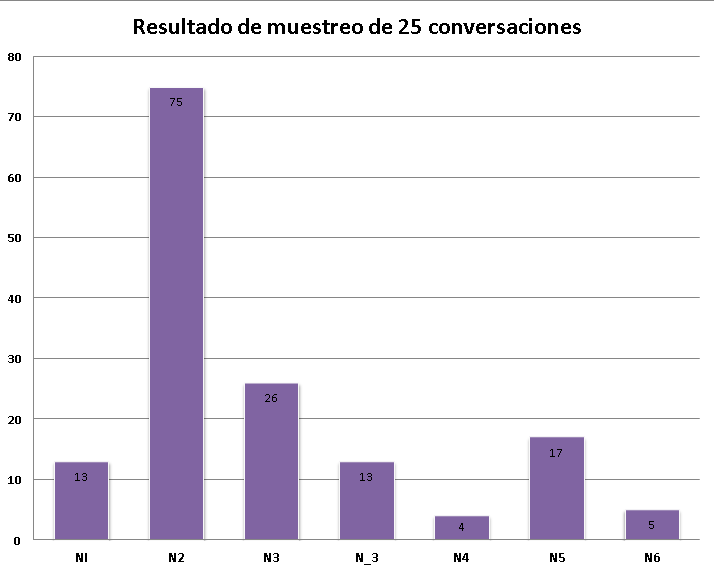
\includegraphics[scale=.3]{images/grafica/ClasificacionNiv}
\caption{Resultados del muestro de 25 conversaciones}
\label{fig:ClasificacionNiv}
\end{center}
\end{figure}


En la tabla \ref{tab:resultadosM} se muestran los resultados que obtuvimos de las 25 conversaciones anteriormente mencionadas. La tabla contiene el n\'umero de conversaciones que se encontraron de las 4 diferentes categor\'ias: No peligrosa, Poco peligrosa, Peligrosa, Muy peligrosa.

\begin{table}
\begin{center}


\begin{tabular}
\hline
Clasificac\'on & Incidencias \\
\hline

No Peligrosa & 7\\
Poco Peligrosa & 0\\
Peligrosa & 1\\
Muy peligrosa & 17\\
\hline
\end{tabular}

\caption{Resultados de muestreo de 25 conversaciones}
\label{tab:resultadosM}
\end{center}
\end{table}

En la figura \ref{fig:ClasificacionConv} podemos observar graficamente la tabla anterior. Los resultados del muestreo de 25 conversaciones muestran que la mayor\'ia de \'estas (17) fueron detectadas como peligrosas.

\begin{figure}[h]
\begin{center}
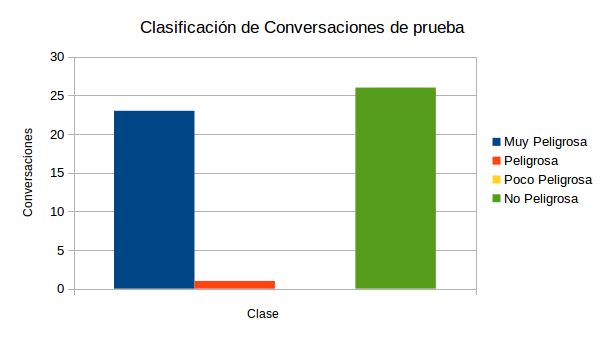
\includegraphics[scale=.3]{images/grafica/ClasificacionConv}
\caption{Resultados del muestro de 25 conversaciones}
\label{fig:ClasificacionConv}
\end{center}
\end{figure}




\chapter{Prototipo 6: Sistema de Mensajer\'ia}
\section{An\'alisis}

\subsection{Descripci\'on}

Este prototipo permite la visualizaci\'on del funcionamiento de la API de an\'alisis mediante un sistema de mensajer\'ia.

\subsection{Objetivo}
Generar un sistema de mensajer\'ia sobre el cual el funcionamiento de la API de an\'alisis ser\'a visualizado. 

\subsection{Caracter\'isticas}

\begin{description}
\item[FEAT1] El usuario puede registrarse al sistema.
\item[FEAT2] El usuario puede ingresar al sistema.
\item[FEAT3] El usuario puede visualizar su lista de contactos.
\item[FEAT4] El usuario puede agregar a otros usuarios a su lista de contactos.
\item[FEAT5] El usuario puede conversar con otros usuarios.
\item[FEAT6] El usuario puede vizualizar si las conversaciones en las cuales ha participado son peligrosas.

\end{description}

\subsection{Restricciones}
\begin{itemize}
\item Prototipo desarrollado con el framework Django 1.7.
\item Desarrollado con python 2.7.
\end{itemize}

\subsection{Casos de uso}

\section{Modelo de casos de uso del sistema de mensajer\'ia}

El siguiente diagrama de casos de uso muestra las acciones que el usuario podr\'a realizar dentro del sistema de mensajer\'ia. El usuario, llamado Contacto, ser\'a capaz de realizar las siguientes actividades:
\begin{itemize}
	\item Registrar de contacto
\item Iniciar sesi\'on
\item Agregar contacto a una lista
\item Enviar mensaje
\item Cerrar sesi\'on
\end{itemize}
	\begin{figure}[htbp!]
		\centering
			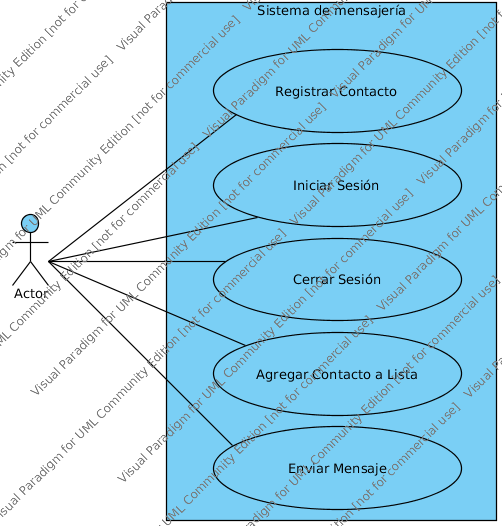
\includegraphics[width=0.8\textwidth]{images/Diagramas/dcasosdeuso}
		\caption{Diagrama de Casos de Uso del sistema de mensajer\'ia.}
	\end{figure}
	
	
	\pagebreak

% \IUref{IUAdmPS}{Administrar Planta de Selección}
% \IUref{IUModPS}{Modificar Planta de Selección}
% \IUref{IUEliPS}{Eliminar Planta de Selección}

% 


% Copie este bloque por cada caso de uso:
%-------------------------------------- COMIENZA descripción del caso de uso.

%\begin{UseCase}[archivo de imágen]{UCX}{Nombre del Caso de uso}{
	\begin{UseCase}{CU3}{Enviar mensaje}{El caso de uso permite al Contacto enviar mensajes de texto a trav\'es de un canal abierto de comunicaci\'on.
	}
		\UCitem{Versi\'on}{0.2}
		\UCitem{Actor}{Contacto}
		\UCitem{Prop\'osito}{Enviar y Almacenar los mensajes escritos enviados entre los usuarios del sistema de mensajer\'ia, para su an\'alisis en el desarrollo de los m\'odulos posteriores.}
		\UCitem{Resumen}{
		El caso de uso permite al usuario enviar mensajes atrav\'es del un canal de comunicacion abierto}
		\UCitem{Entradas}{Mensaje string  (obligatorio)}
		\UCitem{Salidas}{Historial de mensajes enviados y recibidos }
		\UCitem{Precondiciones}{El usuario debera tener un canal de comunicaci\'on abierto.El mensaje no puede estar vac\'io.}
		\UCitem{Postcondiciones}{Los mensajes enviados y recibidos podr\'an ser visualidaos por ambos usuarios que comparten el mismo canal}		
		\UCitem{Autor}{Anah\'i Ruiz D\'iaz}
	\end{UseCase}

	\begin{UCtrayectoria}{Principal}
	
		\UCpaso[\UCactor] El usuario escribe un mensaje dentro de una caja de textos.
		\UCpaso[\UCactor] El usuario da clic en el bot\'on \IUbutton{Enviar} para enviar el mensaje. 

		\UCpaso  El sistema env\'ia y muestra al otro Contacto el mensaje enviado por el usuario.  \Trayref{A}.
		\UCpaso[] Fin del flujo.
				
	\end{UCtrayectoria}
		
		\begin{UCtrayectoriaA}{A}{Mensaje no enviado}
			\UCpaso El sistema muestra una alerta que notifica al usuario que ocurri\'o un error y su mensaje no fue enviado.
			\UCpaso[] El usuario da clic en el bot\'on \IUbutton{Aceptar}.
			\UCpaso[] Fin del flujo.
		\end{UCtrayectoriaA}


%-------------------------------------- TERMINA descripción del caso de uso.
% \IUref{IUAdmPS}{Administrar Planta de Selección}
% \IUref{IUModPS}{Modificar Planta de Selección}
% \IUref{IUEliPS}{Eliminar Planta de Selección}

% 


% Copie este bloque por cada caso de uso:
%-------------------------------------- COMIENZA descripción del caso de uso.

%\begin{UseCase}[archivo de imágen]{UCX}{Nombre del Caso de uso}{
	\begin{UseCase}{CU3}{Enviar mensaje}{El caso de uso permite al Contacto enviar mensajes de texto a trav\'es de un canal abierto de comunicaci\'on.
	}
		\UCitem{Versi\'on}{0.2}
		\UCitem{Actor}{Contacto}
		\UCitem{Prop\'osito}{Enviar y Almacenar los mensajes escritos enviados entre los usuarios del sistema de mensajer\'ia, para su an\'alisis en el desarrollo de los m\'odulos posteriores.}
		\UCitem{Resumen}{
		El caso de uso permite al usuario enviar mensajes atrav\'es del un canal de comunicacion abierto}
		\UCitem{Entradas}{Mensaje string  (obligatorio)}
		\UCitem{Salidas}{Historial de mensajes enviados y recibidos }
		\UCitem{Precondiciones}{El usuario debera tener un canal de comunicaci\'on abierto.El mensaje no puede estar vac\'io.}
		\UCitem{Postcondiciones}{Los mensajes enviados y recibidos podr\'an ser visualidaos por ambos usuarios que comparten el mismo canal}		
		\UCitem{Autor}{Anah\'i Ruiz D\'iaz}
	\end{UseCase}

	\begin{UCtrayectoria}{Principal}
	
		\UCpaso[\UCactor] El usuario escribe un mensaje dentro de una caja de textos.
		\UCpaso[\UCactor] El usuario da clic en el bot\'on \IUbutton{Enviar} para enviar el mensaje. 

		\UCpaso  El sistema env\'ia y muestra al otro Contacto el mensaje enviado por el usuario.  \Trayref{A}.
		\UCpaso[] Fin del flujo.
				
	\end{UCtrayectoria}
		
		\begin{UCtrayectoriaA}{A}{Mensaje no enviado}
			\UCpaso El sistema muestra una alerta que notifica al usuario que ocurri\'o un error y su mensaje no fue enviado.
			\UCpaso[] El usuario da clic en el bot\'on \IUbutton{Aceptar}.
			\UCpaso[] Fin del flujo.
		\end{UCtrayectoriaA}


%-------------------------------------- TERMINA descripción del caso de uso.
% \IUref{IUAdmPS}{Administrar Planta de Selección}
% \IUref{IUModPS}{Modificar Planta de Selección}
% \IUref{IUEliPS}{Eliminar Planta de Selección}

% 


% Copie este bloque por cada caso de uso:
%-------------------------------------- COMIENZA descripción del caso de uso.

%\begin{UseCase}[archivo de imágen]{UCX}{Nombre del Caso de uso}{
	\begin{UseCase}{CU3}{Enviar mensaje}{El caso de uso permite al Contacto enviar mensajes de texto a trav\'es de un canal abierto de comunicaci\'on.
	}
		\UCitem{Versi\'on}{0.2}
		\UCitem{Actor}{Contacto}
		\UCitem{Prop\'osito}{Enviar y Almacenar los mensajes escritos enviados entre los usuarios del sistema de mensajer\'ia, para su an\'alisis en el desarrollo de los m\'odulos posteriores.}
		\UCitem{Resumen}{
		El caso de uso permite al usuario enviar mensajes atrav\'es del un canal de comunicacion abierto}
		\UCitem{Entradas}{Mensaje string  (obligatorio)}
		\UCitem{Salidas}{Historial de mensajes enviados y recibidos }
		\UCitem{Precondiciones}{El usuario debera tener un canal de comunicaci\'on abierto.El mensaje no puede estar vac\'io.}
		\UCitem{Postcondiciones}{Los mensajes enviados y recibidos podr\'an ser visualidaos por ambos usuarios que comparten el mismo canal}		
		\UCitem{Autor}{Anah\'i Ruiz D\'iaz}
	\end{UseCase}

	\begin{UCtrayectoria}{Principal}
	
		\UCpaso[\UCactor] El usuario escribe un mensaje dentro de una caja de textos.
		\UCpaso[\UCactor] El usuario da clic en el bot\'on \IUbutton{Enviar} para enviar el mensaje. 

		\UCpaso  El sistema env\'ia y muestra al otro Contacto el mensaje enviado por el usuario.  \Trayref{A}.
		\UCpaso[] Fin del flujo.
				
	\end{UCtrayectoria}
		
		\begin{UCtrayectoriaA}{A}{Mensaje no enviado}
			\UCpaso El sistema muestra una alerta que notifica al usuario que ocurri\'o un error y su mensaje no fue enviado.
			\UCpaso[] El usuario da clic en el bot\'on \IUbutton{Aceptar}.
			\UCpaso[] Fin del flujo.
		\end{UCtrayectoriaA}


%-------------------------------------- TERMINA descripción del caso de uso.
% \IUref{IUAdmPS}{Administrar Planta de Selección}
% \IUref{IUModPS}{Modificar Planta de Selección}
% \IUref{IUEliPS}{Eliminar Planta de Selección}

% 


% Copie este bloque por cada caso de uso:
%-------------------------------------- COMIENZA descripción del caso de uso.

%\begin{UseCase}[archivo de imágen]{UCX}{Nombre del Caso de uso}{
	\begin{UseCase}{CU3}{Enviar mensaje}{El caso de uso permite al Contacto enviar mensajes de texto a trav\'es de un canal abierto de comunicaci\'on.
	}
		\UCitem{Versi\'on}{0.2}
		\UCitem{Actor}{Contacto}
		\UCitem{Prop\'osito}{Enviar y Almacenar los mensajes escritos enviados entre los usuarios del sistema de mensajer\'ia, para su an\'alisis en el desarrollo de los m\'odulos posteriores.}
		\UCitem{Resumen}{
		El caso de uso permite al usuario enviar mensajes atrav\'es del un canal de comunicacion abierto}
		\UCitem{Entradas}{Mensaje string  (obligatorio)}
		\UCitem{Salidas}{Historial de mensajes enviados y recibidos }
		\UCitem{Precondiciones}{El usuario debera tener un canal de comunicaci\'on abierto.El mensaje no puede estar vac\'io.}
		\UCitem{Postcondiciones}{Los mensajes enviados y recibidos podr\'an ser visualidaos por ambos usuarios que comparten el mismo canal}		
		\UCitem{Autor}{Anah\'i Ruiz D\'iaz}
	\end{UseCase}

	\begin{UCtrayectoria}{Principal}
	
		\UCpaso[\UCactor] El usuario escribe un mensaje dentro de una caja de textos.
		\UCpaso[\UCactor] El usuario da clic en el bot\'on \IUbutton{Enviar} para enviar el mensaje. 

		\UCpaso  El sistema env\'ia y muestra al otro Contacto el mensaje enviado por el usuario.  \Trayref{A}.
		\UCpaso[] Fin del flujo.
				
	\end{UCtrayectoria}
		
		\begin{UCtrayectoriaA}{A}{Mensaje no enviado}
			\UCpaso El sistema muestra una alerta que notifica al usuario que ocurri\'o un error y su mensaje no fue enviado.
			\UCpaso[] El usuario da clic en el bot\'on \IUbutton{Aceptar}.
			\UCpaso[] Fin del flujo.
		\end{UCtrayectoriaA}


%-------------------------------------- TERMINA descripción del caso de uso.
% \IUref{IUAdmPS}{Administrar Planta de Selección}
% \IUref{IUModPS}{Modificar Planta de Selección}
% \IUref{IUEliPS}{Eliminar Planta de Selección}

% 


% Copie este bloque por cada caso de uso:
%-------------------------------------- COMIENZA descripción del caso de uso.

%\begin{UseCase}[archivo de imágen]{UCX}{Nombre del Caso de uso}{
	\begin{UseCase}{CU3}{Enviar mensaje}{El caso de uso permite al Contacto enviar mensajes de texto a trav\'es de un canal abierto de comunicaci\'on.
	}
		\UCitem{Versi\'on}{0.2}
		\UCitem{Actor}{Contacto}
		\UCitem{Prop\'osito}{Enviar y Almacenar los mensajes escritos enviados entre los usuarios del sistema de mensajer\'ia, para su an\'alisis en el desarrollo de los m\'odulos posteriores.}
		\UCitem{Resumen}{
		El caso de uso permite al usuario enviar mensajes atrav\'es del un canal de comunicacion abierto}
		\UCitem{Entradas}{Mensaje string  (obligatorio)}
		\UCitem{Salidas}{Historial de mensajes enviados y recibidos }
		\UCitem{Precondiciones}{El usuario debera tener un canal de comunicaci\'on abierto.El mensaje no puede estar vac\'io.}
		\UCitem{Postcondiciones}{Los mensajes enviados y recibidos podr\'an ser visualidaos por ambos usuarios que comparten el mismo canal}		
		\UCitem{Autor}{Anah\'i Ruiz D\'iaz}
	\end{UseCase}

	\begin{UCtrayectoria}{Principal}
	
		\UCpaso[\UCactor] El usuario escribe un mensaje dentro de una caja de textos.
		\UCpaso[\UCactor] El usuario da clic en el bot\'on \IUbutton{Enviar} para enviar el mensaje. 

		\UCpaso  El sistema env\'ia y muestra al otro Contacto el mensaje enviado por el usuario.  \Trayref{A}.
		\UCpaso[] Fin del flujo.
				
	\end{UCtrayectoria}
		
		\begin{UCtrayectoriaA}{A}{Mensaje no enviado}
			\UCpaso El sistema muestra una alerta que notifica al usuario que ocurri\'o un error y su mensaje no fue enviado.
			\UCpaso[] El usuario da clic en el bot\'on \IUbutton{Aceptar}.
			\UCpaso[] Fin del flujo.
		\end{UCtrayectoriaA}


%-------------------------------------- TERMINA descripción del caso de uso.
\section{Diagrama de clases del sistema de mensajer\'ia}

El siguiente diagrama de clases muestra las clases, con sus respectivos argumentos y m\'etodos, que se pretende implementar para el dise\~no de nuestro sistema de mensajer\'ia. 

Podemos observar que se hace uso de MVC (Model-View-Control), mediante el cual pretendemos agrupar los componentes de la aplicaci\'on en tres niveles l\'ogicos: modelo, vista y controlador.

En el modelo se pretende representar la informaci\'on que el sistema manipulara.

La vista generar\'a una representaci\'on visual del Modelo y muestrar\'a los datos al Contacto, permitiendo que \'este interactuel con el sistema.

Y finalmente el controlador que ser\'a quien responda a eventos o acciones invocadas por el Contacto. 



%	\begin{figure}[htbp!]
%		\centering
%			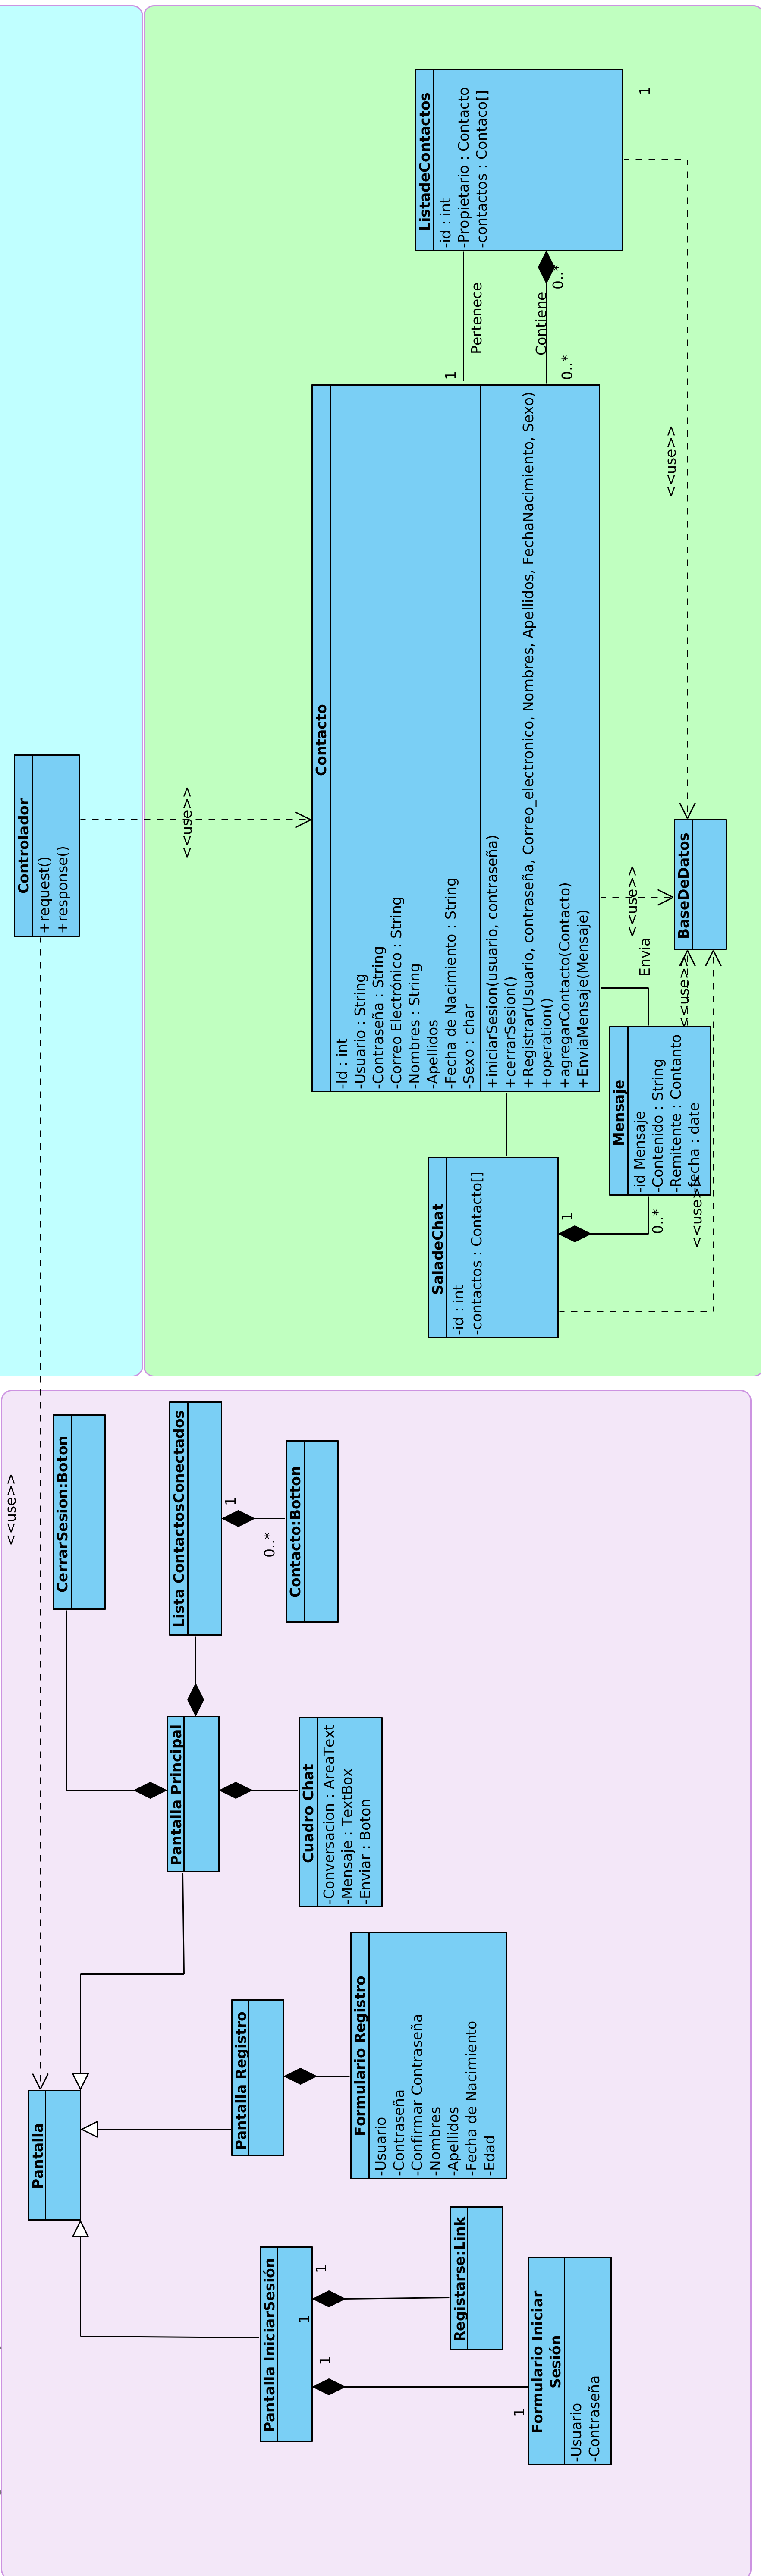
\includegraphics[width=12cm, height=20cm]{images/Diagramas/dclases}
%		\caption{Diagrama de Clases del sistema de mensajer\'ia.}
%	\end{figure}
	
	\begin{figure}[htbp!]
		\centering
			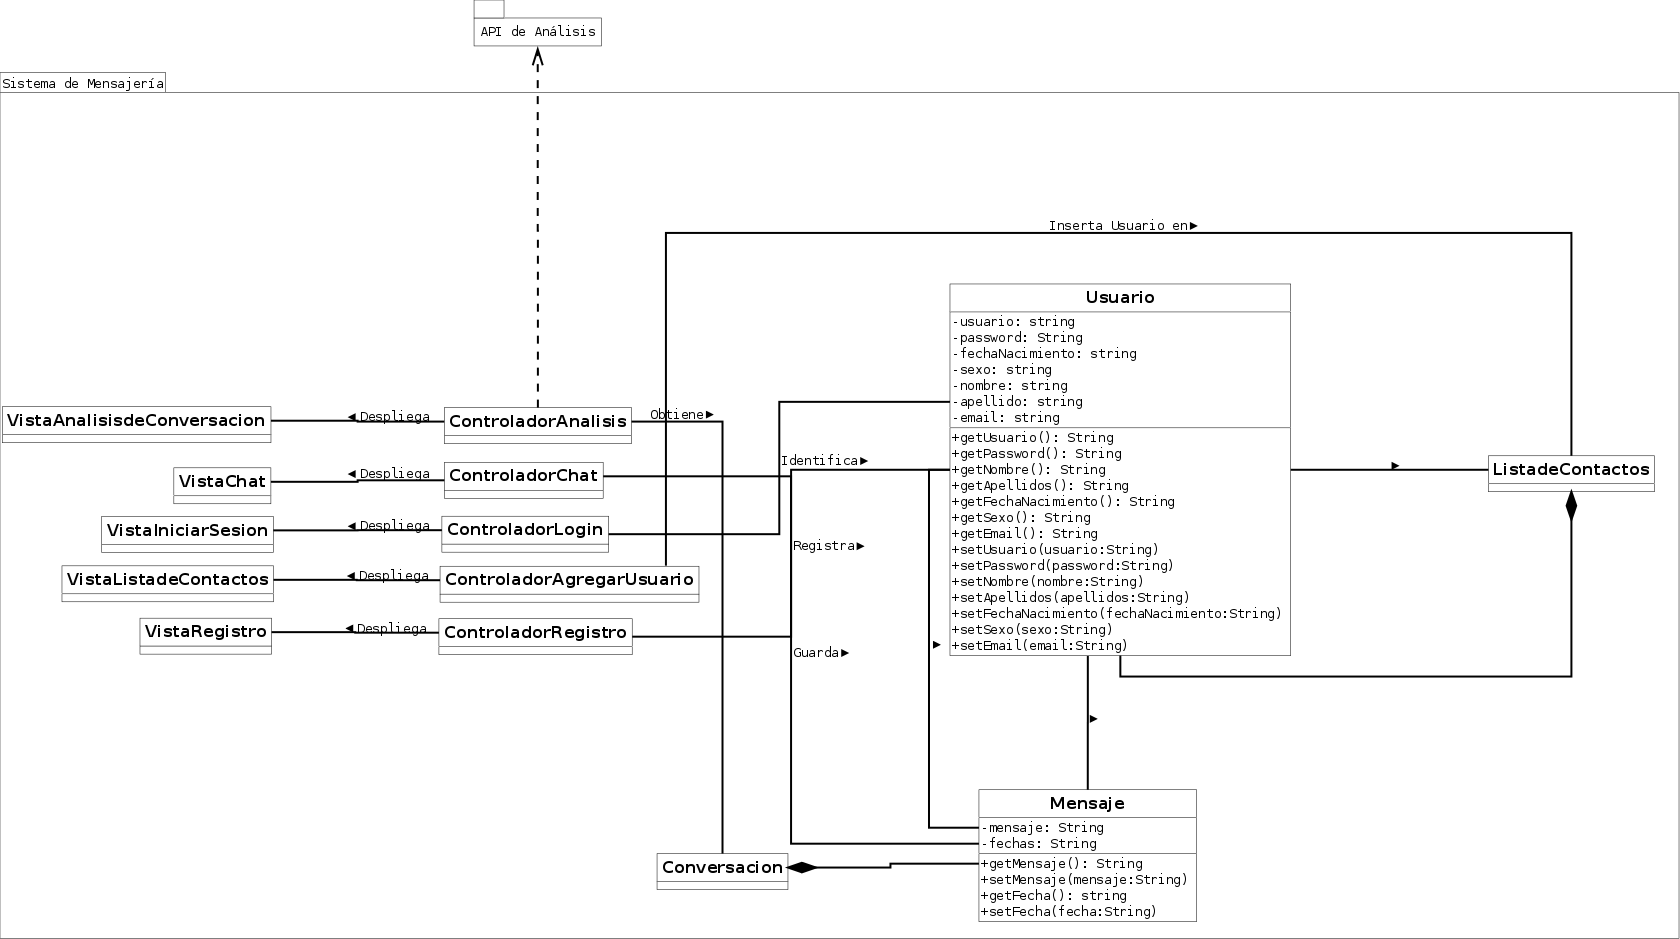
\includegraphics[width=18cm, height=13cm]{images/Diagramas/ddclases}
		\caption{Diagrama de Clases del sistema de mensajer\'ia.}
	\end{figure}
	
	

	
	\pagebreak
\section{Diagrama de paquetes}
La figura \ref{fig:paquetes} muestra c\'omo el chat est\'a conectado con la API de an\'alisis. De esta manera integramos la API que realizamos en los prototipos anteriores con el sistema en general.
\begin{figure}
\includegraphics[scale=.4]{images/diagramapaquetes}
\caption{Diagrama de paquetes del la inetegraci\'on del chat con la API de an\a'lisis}
\label{fig:paquetes}
\end{figure}


\section{Modelo de la interacci\'on del Contacto con el sistema de mensajer\'ia }
\subsection{Diagrama de secuencia del sistema de mensajer\'ia (Iniciar sesi\'on)}
El siguiente diagrama de secuencia muestra las acciones que realiza el sistema y la interacci\'on que se lleva acabo con el usuario en el momento en el que un Contacto realiza el inicio de sesi\'on.


	\begin{figure}[htbp!]
		\centering
			\includegraphics[width=15cm, height=20cm]{images/Diagramas/SecIniciarSesion}
		\caption{Diagrama de Secuencia Iniciar Sesi\'on.}
	\end{figure}
	\pagebreak	
\subsection{Diagrama de secuencia del sistema de mensajer\'ia (Registro de Contacto)}
El siguiente diagrama de secuencia muestra las acciones que realiza el sistema en el momento en el que un usuario nuevo desea registrarse en el sistema para su posterior uso.
	
	
	\begin{figure}[htbp!]
		\centering
			\includegraphics[width=15cm, height=20cm]{images/Diagramas/SecRegistro}
		\caption{Diagrama de Secuencia Registro.}
	\end{figure}
	\pagebreak
\subsection{Diagrama de secuencia del sistema de mensajer\'ia (Agregar Contacto)}
El siguiente diagrama de secuencia muestra las acciones que realiza el sistema cuando un usuario desea agregar a su lista de contactos un nuevo Contacto.
	
	
	\begin{figure}[htbp!]
		\centering
			\includegraphics[width=15cm, height=20cm]{images/Diagramas/SecAdd}
		\caption{Diagrama de Secuencia Agregar contacto.}
	\end{figure}
		\pagebreak
\subsection{Diagrama de secuencia del sistema de mensajer\'ia (Enviar mensaje)}
El siguiente diagrama de secuencia muestra los pasos que lleva acabo el sistema en el momento en el que un Contacto decide enviar un mensaje a otro Contacto.
		
		\begin{figure}[htbp!]
		\centering
			\includegraphics[width=15cm, height=20cm]{images/Diagramas/SecEnviar}
		\caption{Diagrama de Secuencia Enviar Mensaje.}
	\end{figure}
		\pagebreak
	\subsection{Diagrama de secuencia del sistema de mensajer\'ia (Cerrar sesi\'on)}
El siguiente diagrama de secuencia muestra las acciones que realiza el sistema y la interacci\'on que se lleva acabo con el usuario en el momento en el que un Contacto desea cerrar su sesi\'on.
	
			\begin{figure}[htbp!]
		\centering
			\includegraphics[width=15cm, height=20cm]{images/Diagramas/SecCerrar}
		\caption{Diagrama de Secuencia Cerrar sesi\'on.}
	\end{figure}

	
	\pagebreak

		
		\subsection{IU1 Pantalla de Iniciar sesi\'on}

\subsubsection{Objetivo}
	Verificar si el usuario que est\'a intentando entrar al sistema sea el correcto y ya se encuentra registrado en el sistema de mensajer\'ia.

\subsubsection{Dise\~no}
	Esta pantalla aparece al ingresar al sistema de mensajer\'ia. 

	\begin{figure}[htbp!]
		\centering
			\includegraphics[width=0.9\textwidth]{images/Modulo1/Login}
		\caption{Pantalla de inicio de sesi\'on.}
	\end{figure}

\subsubsection{Salidas}
Ninguna


\subsubsection{Entradas}
\begin{Citemize}

\item Usuario 
\item Contrase\~na
\end{Citemize}

\subsubsection{Comandos}
\begin{itemize}
	\item \IUbutton{Login}: Verifica que el usuario se encuentre registrado en la base de datos y de ser as\'i verifica que la contrase\~na corresponda al usuario. 
	\item \IUbutton{Reg\'istrate}: Muestra el formulario que el usuario necesita llenar para poder registrarse en el sistema.
\end{itemize}

\subsubsection{Mensajes}
	\begin{Citemize}
		\item {\bf MSG1} Forbidden.	\end{Citemize}
		
	\pagebreak		%%%%%%%%%%%%%%%%%%%%%%%%%%%%%%%%%%%%%%%%%%%%%%%%%%
		
		\subsection{IU2 Pantalla de Registro de usuario}

\subsubsection{Objetivo}
	Registrar a un usuario con el objetivo de obtener sus datos principales y que \'este posteriormente pueda hacer uso del sistema de mensajer\'ia.

\subsubsection{Dise\~no}
	Esta pantalla aparece al dar clic en el bot\'on \IUbutton{Registrarte} que se encuentra al final de la pantalla de inicio.

	\begin{figure}[htbp!]
		\centering
			\includegraphics[width=0.8\textwidth]{images/Modulo1/Registro}
		\caption{Pantalla de registro de usuario.}
	\end{figure}

\subsubsection{Salidas}
	\begin{Citemize}
		\item {\bf MSG1} Ha sido registrado correctamente.	
	\end{Citemize}
	


\subsubsection{Entradas}
\begin{Citemize}

\item Usuario 
\item Contrase\~na
\item Correo electr\'onico 
\item Nombre
\item Apellidos
\item Fecha de nacimiento
\item Sexo
\end{Citemize}

\subsubsection{Comandos}
\begin{itemize}
	\item \IUbutton{Enviar}: Ingresa los datos del usuario a la base de datos, si estos fueron ingresados correctamente muestra el mensaje de registro exitoso. \end{itemize}
	\begin{figure}[htbp!]
		\centering
			\includegraphics[width=0.9\textwidth]{images/Modulo1/SalidaRegistro}
		\caption{Mensaje de registro exitoso.}
	\end{figure}
\subsubsection{Mensajes}
	\begin{Citemize}
		\item {\bf MSG2} This field is required.	\end{Citemize}
		
			\pagebreak%%%%%%%%%%%%%%%%%%%%%%%%%%%%%%%%%%%%%%%%%%%%%%%%%%
	\subsection{IU3 Pantalla de Conversaciones}

\subsubsection{Objetivo}
	El objetivo de esta pantalla es que el usuario pueda visualizar las conversaciones que tiene, es decir, los contactos que forman parte de su lista.

\subsubsection{Dise\~no}
	Esta pantalla aparece al iniciar sesi\'on correctamente.

	\begin{figure}[htbp!]
		\centering
			\includegraphics[width=0.9\textwidth]{images/Modulo1/Conversaciones}
		\caption{Pantalla de conversaciones}
	\end{figure}

\subsubsection{Salidas}
Lista de Contactos (conversaciones)


\subsubsection{Entradas}
\begin{Citemize}


\item Contacto
\end{Citemize}
\subsubsection{Comandos}
\begin{itemize}
			\item \IUbutton{"Contacto"}: Muestra la conversaci\'on del Contacto seleccionado y permite el intercambio de mensajes.
			\item \IUbutton{Cerrar sesi\'on}: Termina la sesi\'on y regresa a la p\'agina de inicio.
	\end{itemize}

\subsubsection{Mensajes}
Ninguno

		
	\pagebreak		%%%%%%%%%%%%%%%%%%%%%%%%%%%%%%%%%%%%%%%%%%%%%%%%%%
	
	
	
		
		\subsection{IU4 Pantalla del Sistema de Mensajer\'ia}

\subsubsection{Objetivo}
	El objetivo de esta pantalla es que el usuario pueda enviar y recibir mensajes de otros usuarios conectados.

\subsubsection{Dise\~no}
	Esta pantalla aparece al elegir el Contacto con el cual se desea intercambiar mensajes o analizar conversaciones pasadas.

	\begin{figure}[htbp!]
		\centering
			\includegraphics[width=0.9\textwidth]{images/Modulo1/Chat}
		\caption{Pantalla del sistema de mensajer\'ia}
	\end{figure}

\subsubsection{Salidas}
Conversaci\'on


\subsubsection{Entradas}
\begin{Citemize}

\item Mensaje 

\end{Citemize}
\subsubsection{Comandos}
\begin{itemize}
	\item \IUbutton{Enviar Mensaje}: Se env\'ia la cadena de caracteres contenida en el campo "Mensaje" a otro usuario del sistema. 
	\item \IUbutton{Analizar Conversaci\'on}: Muestra el an\'alisis de la conversaci\'on actualmente mostrada.
		\item \IUbutton{Cerrar sesi\'on}: Termina la sesi\'on y regresa a la p\'agina de inicio.
	\end{itemize}

\subsubsection{Mensajes}
Ninguno




	\pagebreak%%%%%%%%%%%%%%%%%%%%%%%%%%%%%%%%%%%%%%%%%%%%%%%%%%

	
	
	
	
			\subsection{IU5 Pantalla del An\'alisis (Gr\'afica)}

\subsubsection{Objetivo}
	El objetivo de esta pantalla es que el usuario pueda visualizar los resultados del an\'alisis realizado a la conversaci\'on solicitado.

\subsubsection{Dise\~no}
	Esta pantalla aparece despu\'es de solicitar el an\'alisis de la conversaci\'on en la pantalla del chat.

	\begin{figure}[htbp!]
		\centering
			\includegraphics[width=0.9\textwidth]{images/Modulo1/GraficaAnalisis}
		\caption{Pantalla del An\'alisis (Gr\'afica)}
	\end{figure}

\subsubsection{Salidas}
Ninguna


\subsubsection{Entradas}
Ninguna
\subsubsection{Comandos}
Ninguno
\subsubsection{Mensajes}
Resultados del an\'alisis de la conversaci\'on 

\begin{figure}[htbp!]
		\centering
			\includegraphics[width=0.9\textwidth]{images/Modulo1/InsidenciasNivel}
		\caption{Pantalla del An\'alisis (Incidencias)}
	\end{figure}



	\pagebreak%%%%%%%%%%%%%%%%%%%%%%%%%%%%%%%%%%%%%%%%%%%%%%%%%%



\chapter{Conclusiones}
%Los objetivos que logramos durante el desarrollo de nuestro sistema son los siguientes:
%
%Aplicaci\'on para el intercambio de conversaciones
%API para el an\'alisis de conversaciones
%Aplicaci\'on para el procesamiento de texto
%Aplicaci\'on que sirva como conexi\'on entre los m\'odulos del sistema
%Un set de pruebas de desempeño del sistema para verificar su eficiencia
%
%Cumpliendo con estos objetivos se logra desarrollar un sistema capaz de analizar y clasificar texto en diferentes categorias a partir de un conjunto de datos estadisticos mediante reconocimiento de patrones, aprendizaje maquina y mineria de datos. Cuyo fin es el clasificar una conversaci\'on como no peligrosa o determinar un grado de peligrosidad de estas.  
%
%A trav\'es de los prototipos que desarrollamos fue posible alcanzar los objetivos. 
%
%Con el prototipo 1 logramos extrar las careceteristicas de una manera que permitiera generar datos para la desici\'on del clasificador.
%
%El prototipo 2 plantemos un esquema para buscar palabras de car\'acter sexual.
%
%En el prototipo 3 obtuvimos un clasificador con una efectividad en el valor de $F_1score= 0.9743$ conjunto de entrenamiento contra un valor de $F_1score= 0.87$ en el conjunto de validaci\'on.
%
%El prototipo 4 agrupo el clasificador del prototipo 3 para conjuntarlo con las caracter\'isticas que obtuvimos en el prototipo 1.
%
%En el  prototipo n\'umero 5 obtuvimos desarrollamos un sistema de mensajer\'ia y de manera exitosa logramos unir est\'e prototipo con la API de desici\'on.

%PRIMERA CONCLUSION%

%Consideramos que la metodolog\'ia que elegimos nos fue bastante \'util ya que nos proporciona la oportunidad de desarrollar primero las partes del sistema que son m\'as visibles y presentarlas para despu\'es continuar con el desarrollo del siguiente prototipo basandonos en la retroalimentaci\'on que recibamos. 

%La parte del an\'alisis nos fue de gran ayuda y utilidad ya que nos da la oportunidad de visualizar aspectos del sistema que no ten\'iamos contemplados en primera instancia. Tambi\'en nos permite organizar de una manera m\'as optima el desarrollo del prototipo.

%A pesar de que el M\'odulo 1 "Sistema de mensajer\'ia" no es el enfoque principal de nuestro Trabajo Terminal, nos tom\'o un lapso considerable de tiempo debido al aprendizaje de la herramienta en la que se pretend\'ia desarrollarse. 

%Con respecto al procesamiento del texto, notamos que la eliminaci\'on de las stopwords nos ayuda a que la lista de palabras se haga m\'as peque\~na, lo cual mejora la eficiencia ya que hay una selecci\'on mejor de palabras claves que s\'i nos son \'utiles.

%En cuanto al stemming y la lematizaci\'on se tiene la ventaja de que mejora la eficiencia, se comprimen los \'indices y se mejora el recall y la desventaja es que se puede perder la informaci\'on sobre los t\'erminos. 

%Debido a que el lenguaje de programaci\'on que elegimos para desarrollar nuestro sistema fue Phyton, la documentaci\'on de Natural Language Toolkit (NLTK) fue una herramienta que nos ampli\'o la visi\'on de las cosas y nos ayud\'o en cuanto al procesamiento de texto.

%Finalmente podemos agregar que la organizaci\'on, el trabajo en equipo, la comunicaci\'on y la convivencia son puntos culminantes para que se lleve acabo un buen y sano desarrollo de todo sistema.

La API de este sistema puede ser utilizada como herramienta para la detecci\'on de conversaciones peligrosas (\textit{online grooming}) o ver como \'estas se  comportan de acuerdo a los 6 niveles de  caracterizaci\'on \cite{articulo}. Las conversaciones con las que se trabaj\'o y que  fueron marcadas como peligrosas en el conjunto de entrenamiento as\'i como para el conjunto de pruebas  fueron extra\'idas de un sitio alojado en Estados Unidos en el que son publicadas conversaciones reales de personas que se hacen pasar por ni\~nos para detectar y capturar pederastas en Internet. \cite{perverd}
%Bajo estad\'isticas de palabras la b\'usqueda de frases de acuerdo a los niveles marcados en el art\'iculo ya antes citado, se pudieron an\'alizar y procesar aquellas conversaciones.

Los objetivos logrados al desarrollar el presente trabajo terminal son:

\begin{itemize}
\item Una Aplicaci\'on para el procesamiento de texto, encargada de la b\'usqueda de frases y palabras relacionadas con nuestro caso de estudio (\textit{online grooming}).
\item El desarrollo de una API para el an\'alisis de conversaciones, la cual aplica el algoritmo de regresi\'on log\'istica y Red Neuronal Perceptr\'on Multicapa entrenada con el algoritmo de \textit{backpropagation} para clasificar una conversaci\'on como: Muy Peligrosa, Peligrosa, Poco Peligrosa o No peligrosa. \'Esta se llev\'o acabo mediante el desarrollo de los siguientes prototipos:

En el prototipo 1 se lograron extraer, contar y hacer una estad\'istica de las frases de los niveles 1,2,3,4 y 6 utilizando el \textit{stem} de palabras clave dependiendo del nivel que se quiera analizar.

En el prototipo 2 se plante\'o un esquema para buscar, contar y hacer una estad\'istica de palabras de car\'acter sexual. En este prototipo se definieron los \textit{stems} de las palabras que son los descripto\'res del clasificador del prototipo 3.

En el prototipo 3 se implement\'o un clasificador utilizando el algoritmo de regresi\'on log\'istica. 

El prototipo 4 implementa una Red neuronal perceptr\'on multicapa para tomar la decisi\'on de clasificar las conversaciones como: muy peligrosa, peligrosa, poco peligrosa y no peligrosa. La red neuronal fue entrenada con el algoritmo de \textit{backpropagation}.

En el  prototipo n\'umero 5 se hace la uni\'on de los clasificadores de conversaciones con contexto sexual y el clasificador de niveles de caracterizaci\'on de las conversaciones. Este prototipo es la integraci\'on de la API.


\item Un set de pruebas de desempe\~no del sistema. En la cual se tienen metr\'icas para medir la eficiciencia del sistema. La efectividad del protocolo 3 puede ser comprobada con las matrices de validaci\'on.  Para el conjunto de entrenamiento se obtuvo una efectividad de 0.9743 para la m\'etrica  de $F_1score$ mientras que para el  conjunto de entrenamiento se obtuvo un valor de 0.87 para $F_1score$ en el conjunto de validaci\'on.
La eficiencia del prototipo 4 medida con la m\'etrica de $F_1score$  es de 1.

\item Una aplicaci\'on para el intercambio de conversaciones la cual sirve como un simulador de un \textit{chat} real. 

\item Se lograron integrar diversas herramientas y tecnolog\'ias con ayuda de las cuales se pudieron cumplir los objetivos planteados al inicio del trabajo.

\end{itemize}











\section{Trabajo a Futuro}

   \begin{itemize}
\item Implementar un mecanismo que permita identificar la edad de acuerdo al vocabulario utilizado por los remitentes de los mensajes.
\item Ampliar las restricciones para que esta herramienta pueda ser aplicada en alguna red social como: \textit{Facebook, Whatsapp, Telegram}, o en algun \textit{chat} p\'ublico.
%\item Se us\'o la API con una aplicaci\'on m\'ovil.
\item Definir una ontolog\'ia de catacter sexual que permita la clasificaci\'on de conversaciones peligrosas mediante el contexto.
\item Definir una acci\'on de identificaci\'on al agresosr.
\item Probar la API con otros algortimos de clasificaci\'on y comparar la eficiencia.
\item Delimitar el diccionario de frases y palabras de acuerdo a regiones geogr\'aficas.
\item Identificar abreviaciones y \textit{emoticones} populares en el texto e identificar su significado.




%Integraci\'on de diversas herramientas (conclusion)

%Dependencia en diagrama debajo del de clases
%Diagrama de clases del clasificador
\end{itemize}








\appendix
\chapter{Conversaciones Peligrosas}\label{app:conversaciones}
En este ap\'endice se anexan las conversaciones peligrosas con las cuales fueron extraidas las caracter\'isticas para los clasificadores.
\section{Conversaci\'on 1.txt}

\begin{verbatim}
boxbody00 (01/23/07 6:35:41 PM): eres sexy
Decoy Name (01/23/07 6:38:33 PM): jajaja edad, sexo, localidad
boxbody00 (01/23/07 6:38:40 PM): 27 hombre Lawton
boxbody00 (01/23/07 6:38:43 PM): ¿y tú?
Decoy Name (01/23/07 6:38:50 PM): 13, mujer, OK
boxbody00 (01/23/07 6:39:06 PM): ¿de qué quieres hablar?
Decoy Name (01/23/07 6:39:23 PM): no lo sé jaja
boxbody00 (01/23/07 6:39:34 PM): ¿tienes más fotos?
Decoy Name (01/23/07 6:40:05 PM): sí en mi perfil de myspace
boxbody00 (01/23/07 6:40:14 PM): ¿ouedo ver?
Decoy Name (01/23/07 6:40:27 PM): www.myspace.com/Decoy Name
boxbody00 (01/23/07 6:41:19 PM): ¿cuál es tu nombre de usuario?
Decoy Name (01/23/07 6:41:39 PM): ¿para qué?
boxbody00 (01/23/07 6:41:52 PM): entonces te buscaré en MySpace
Decoy Name (01/23/07 6:42:31 PM): Decoy Name
Decoy Name (01/23/07 6:42:37 PM): sólo te daré la liga jajaja
boxbody00 (01/23/07 6:43:29 PM): ¿puedo preguntarte algo?
Decoy Name (01/23/07 6:43:44 PM): sí
Decoy Name (01/23/07 6:43:45 PM): qué
boxbody00 (01/23/07 6:43:50 PM): ¿qué estás usando?
Decoy Name (01/23/07 6:44:03 PM): jaja pantalón de mezclilla y playera
boxbody00 (01/23/07 6:44:11 PM): ¿están ajustadas?
Decoy Name (01/23/07 6:44:15 PM): mi nombre es Eva ¿cuál es el tuyo?
boxbody00 (01/23/07 6:44:34 PM): John
Decoy Name (01/23/07 6:44:55 PM): gusto en conocerte 
boxbody00 (01/23/07 6:45:10 PM): gusto también, entonces ¿tu ropa es ajustada?
Decoy Name (01/23/07 6:45:30 PM): supongo jajaja
Decoy Name (01/23/07 6:45:33 PM): ¿puedo agregarte?
boxbody00 (01/23/07 6:45:38 PM): sí
boxbody00 (01/23/07 6:46:15 PM): ¿qué tan grandes son tus pechos?
Decoy Name (01/23/07 6:46:49 PM): ¿a qué te refieres?
boxbody00 (01/23/07 6:47:05 PM): ¿cuál es la medida de tus tetas? 
Decoy Name (01/23/07 6:47:22 PM): 32b jaja
Decoy Name (01/23/07 6:47:24 PM): ¿por qué?
boxbody00 (01/23/07 6:47:34 PM): porque me encantaría chuparlas
Decoy Name (01/23/07 6:47:51 PM): jajaja ¿de verdad?
boxbody00 (01/23/07 6:48:01 PM): ¿me ayudas a venirme?
Decoy Name (01/23/07 6:48:13 PM): ¿a qué te refieres?
boxbody00 (01/23/07 6:48:23 PM): quieres hablar sucio, para que pueda masturbarme
Decoy Name (01/23/07 6:48:33 PM): ewww. Te refieres cibernéticamente
Decoy Name (01/23/07 6:48:36 PM): eso es asqueroso 
boxbody00 (01/23/07 6:48:44 PM): podemos tener sexo por teléfono
Decoy Name (01/23/07 6:49:07 PM): ewww pero real es mejor
boxbody00 (01/23/07 6:49:19 PM): ¿de dónde eres?
boxbody00 (01/23/07 6:50:48 PM): podemos vernos en algún lugar y tener sexo
Decoy Name (01/23/07 6:51:30 PM): jajaja no lo he hecho aún
Decoy Name (01/23/07 6:51:36 PM): quizá puedas asesinarme o algo
boxbody00 (01/23/07 6:51:52 PM): no soy ese tipo de persona, por favor ¿nos podemos ver?
Decoy Name (01/23/07 6:52:28 PM): jaja podría ser bonito si te conociera antes
Decoy Name (01/23/07 6:52:55 PM): ¿de verdad quieres tener sexo conmigo?
boxbody00 (01/23/07 6:53:08 PM): Diablos, sí
Decoy Name (01/23/07 6:53:21 PM): jajaja wow
boxbody00 (01/23/07 6:53:55 PM): por favor
Decoy Name (01/23/07 6:54:01 PM): qué
boxbody00 (01/23/07 6:54:19 PM): ¿podemos tener sexo?
Decoy Name (01/23/07 6:54:32 PM): jaja sería bueno
boxbody00 (01/23/07 6:54:39 PM): esta noche
Decoy Name (01/23/07 6:54:56 PM): jaja no esta noche, mis tíos están en casa
Decoy Name (01/23/07 6:55:20 PM): ellos irán a Austin al Super Bowl este fin de semana
boxbody00 (01/23/07 6:55:41 PM): ¿por qué no puedes esta noche?
Decoy Name (01/23/07 6:55:52 PM): porque ellos están en casa jaja
boxbody00 (01/23/07 6:56:16 PM): puedes irte
Decoy Name (01/23/07 6:56:28 PM): jajaja me metería en problemas
boxbody00 (01/23/07 6:56:45 PM): ¿en dónde quieres que me venga?
Decoy Name (01/23/07 6:57:04 PM): jajaja ¿a qué te refieres?
boxbody00 (01/23/07 6:57:12 PM): ¿sabes lo que es venirse?
Decoy Name (01/23/07 6:57:27 PM): jajaja sí, supongo
boxbody00 (01/23/07 6:57:49 PM): es la cosa que deja a las niñas embarazadas
Decoy Name (01/23/07 6:58:06 PM): jajaja 
Decoy Name (01/23/07 6:58:06 PM): bien
boxbody00 (01/23/07 6:58:14 PM): ¿dónde quieres?
Decoy Name (01/23/07 6:58:25 PM): no lo sé jaja
boxbody00 (01/23/07 6:58:32 PM): ¿has mamado un pene?
Decoy Name (01/23/07 6:58:48 PM): lo hice una vez
boxbody00 (01/23/07 6:58:59 PM): ¿te gustó?
Decoy Name (01/23/07 6:59:05 PM): jajaja sí, fue bueno
boxbody00 (01/23/07 6:59:14 PM): ¿te tragaste su venida?
Decoy Name (01/23/07 6:59:32 PM): no
boxbody00 (01/23/07 6:59:42 PM): ¿por qué no?
Decoy Name (01/23/07 6:59:52 PM): no lo sé
Decoy Name (01/23/07 6:59:54 PM): jaja él no lo pidió
boxbody00 (01/23/07 7:00:44 PM): ¿quieres tragarte la mía?
Decoy Name (01/23/07 7:00:54 PM): no lo sé, ¿quieres?
boxbody00 (01/23/07 7:01:00 PM): sí
Decoy Name (01/23/07 7:01:18 PM): sería bueno
boxbody00 (01/23/07 7:01:35 PM): ¿puedo tener una foto tuya desnuda?
Decoy Name (01/23/07 7:01:54 PM): ¿me enseñarás tú una?
boxbody00 (01/23/07 7:02:02 PM): no
Decoy Name (01/23/07 7:02:21 PM): sería bueno jaja
Decoy Name (01/23/07 7:02:29 PM): si tú no me enseñas
boxbody00 (01/23/07 7:02:52 PM): nosotros nos podemos tomar fotos con sexo
Decoy Name (01/23/07 7:03:14 PM): huh
boxbody00 (01/23/07 7:04:00 PM): podemos tomarnos fotos teniendo sexo y tenerlas para verlas
Decoy Name (01/23/07 7:04:11 PM): jajaja
boxbody00 (01/23/07 7:04:30 PM): mi pene está duro
Decoy Name (01/23/07 7:04:58 PM): jajaja ¿de verdad?
boxbody00 (01/23/07 7:05:06 PM): sí
Decoy Name (01/23/07 7:05:22 PM): jaja bien
boxbody00 (01/23/07 7:05:37 PM): ¿tienes celular?
Decoy Name (01/23/07 7:05:37 PM): lo siento
Decoy Name (01/23/07 7:08:11 PM): tengo que irme jaja
boxbody00 (01/23/07 7:08:34 PM): ¿tienes celular?
Decoy Name (01/23/07 7:08:39 PM): sí
boxbody00 (01/23/07 7:08:51 PM): ¿tiene cámara?
Decoy Name (01/23/07 7:09:10 PM): sí jajaja
boxbody00 (01/23/07 7:09:24 PM): ¿me puedes enviar fotos de ti desnuda?
Decoy Name (01/23/07 7:09:29 PM): NO
Decoy Name (01/23/07 7:09:30 PM): jajaja
Decoy Name (01/23/07 7:09:35 PM): podrías hacer algo con ellas
boxbody00 (01/23/07 7:09:45 PM): sólo masturbarme
Decoy Name (01/23/07 7:09:53 PM): jajaja de ninguna manera amigo
boxbody00 (01/23/07 7:10:00 PM): por favor sólo una
Decoy Name (01/23/07 7:10:00 PM): me puedes meter en problemas
boxbody00 (01/23/07 7:10:19 PM): ¿cómo te metería en problemas la eliminaré cuando la envíes?
Decoy Name (01/23/07 7:10:29 PM): de ninguna manera

\end{verbatim}
\section{Conversaci\'on 2.txt}

\begin{verbatim}
dicksobig69 (01/28/08 6:30:31 PM): ¿bien, viste mi nombre de yahoo verdad, bebé?
tammytalkslotz (01/28/08 6:30:51 PM): sí
dicksobig69 (01/28/08 6:31:44 PM): ¿sabes lo que significa?
tammytalkslotz (01/28/08 6:32:04 PM): sí
tammytalkslotz (01/28/08 6:32:18 PM): lo puedo leer
dicksobig69 (01/28/08 6:33:04 PM): bueno si quieres ver si es cierto puedes ir a mi perfil y ver
tammytalkslotz (01/28/08 6:33:19 PM): bien
dicksobig69 (01/28/08 6:33:51 PM): después me dices qué piensas, bebé
tammytalkslotz (01/28/08 6:33:59 PM): bien
tammytalkslotz (01/28/08 6:34:56 PM): ooo
tammytalkslotz (01/28/08 6:35:16 PM): ¿eso es tuyo?
dicksobig69 (01/28/08 6:35:25 PM): sí, bebé
tammytalkslotz (01/28/08 6:35:32 PM): ooo
tammytalkslotz (01/28/08 6:35:44 PM): es grande
dicksobig69 (01/28/08 6:36:32 PM): te sonrojas ante él, ¿verdad bebé?
tammytalkslotz (01/28/08 6:36:41 PM): sí
tammytalkslotz (01/28/08 6:36:59 PM): nunca había visto uno antes
dicksobig69 (01/28/08 6:37:04 PM): ¿de verdad?
tammytalkslotz (01/28/08 6:37:14 PM): sí
dicksobig69 (01/28/08 6:37:48 PM): si estuvieras aquí ¿me enseñarías lo que podrías hacer, bebé?
tammytalkslotz (01/28/08 6:37:55 PM): sí
dicksobig69 (01/28/08 6:38:45 PM): sit e pidiera que lo agarraras ¿lo harías bebé?
tammytalkslotz (01/28/08 6:39:13 PM): ¿quieres que lo haga?
dicksobig69 (01/28/08 6:39:23 PM): seguro, bebé
tammytalkslotz (01/28/08 6:39:41 PM): ¿de verdad?
dicksobig69 (01/28/08 6:39:55 PM): ¿tú quieres bebé?
tammytalkslotz (01/28/08 6:40:10 PM): sí
dicksobig69 (01/28/08 6:40:51 PM): entonces si te pido que lo agarres ¿lo harías?
tammytalkslotz (01/28/08 6:41:16 PM): quizá si me lo pides
dicksobig69 (01/28/08 6:41:41 PM): bien, bebé
tammytalkslotz (01/28/08 6:41:49 PM): bien
dicksobig69 (01/28/08 6:42:43 PM): ¿cómo me gusta que me llames, bebé?
tammytalkslotz (01/28/08 6:42:55 PM): oh lo siento, papi
dicksobig69 (01/28/08 6:43:12 PM): bien, bebé
tammytalkslotz (01/28/08 6:43:37 PM): bien, papi
dicksobig69 (01/28/08 6:43:41 PM): ¿todavía estás viendo la foto?
tammytalkslotz (01/28/08 6:43:53 PM): no
tammytalkslotz (01/28/08 6:43:56 PM): jaja
dicksobig69 (01/28/08 6:44:07 PM): ¿por qué no?
tammytalkslotz (01/28/08 6:44:30 PM): porque
dicksobig69 (01/28/08 6:44:45 PM): ¿por qué, bebe?
tammytalkslotz (01/28/08 6:44:52 PM): porque
dicksobig69 (01/28/08 6:45:06 PM): vela otra vez, bebé
tammytalkslotz (01/28/08 6:45:52 PM): ¿quieres que la vea?
dicksobig69 (01/28/08 6:46:03 PM): sí bebé
tammytalkslotz (01/28/08 6:46:10 PM): bien
tammytalkslotz (01/28/08 6:47:02 PM): ya lo hice
dicksobig69 (01/28/08 6:47:27 PM): Buena chica
tammytalkslotz (01/28/08 6:47:33 PM): bien
dicksobig69 (01/28/08 6:48:13 PM): ¿qué si te pidiera que pusieras tu boca en mi pene, bebé?
tammytalkslotz (01/28/08 6:48:45 PM): nunce lo he hecho antes
dicksobig69 (01/28/08 6:49:07 PM): bien, pero ¿lo harías bebé?
tammytalkslotz (01/28/08 6:49:13 PM): sí
tammytalkslotz (01/28/08 6:49:30 PM): ¿a las chicas les gusta hacer eso?
dicksobig69 (01/28/08 6:50:00 PM): sí, normalmente empiezan a tu edad bebé
tammytalkslotz (01/28/08 6:50:07 PM): ¿de verdad?
dicksobig69 (01/28/08 6:50:50 PM): sí, estoy seguro de que las chicas en tu escuela ya empezaron a hacer eso, probablemente las más populares
tammytalkslotz (01/28/08 6:50:58 PM): ooo
tammytalkslotz (01/28/08 6:51:03 PM): bien
dicksobig69 (01/28/08 6:51:57 PM): bien, ¿eres mi chica ahora?
tammytalkslotz (01/28/08 6:52:16 PM): sí
dicksobig69 (01/28/08 6:53:03 PM): entonces ¿podrías tu boca en mi pene, bebé?
tammytalkslotz (01/28/08 6:54:03 PM): si tú quieres
tammytalkslotz (01/28/08 6:55:08 PM): ¿estás ahí?
dicksobig69 (01/28/08 6:55:22 PM): me encantaría que lo hicieras bebé
tammytalkslotz (01/28/08 6:56:02 PM): bien
tammytalkslotz (01/28/08 6:56:09 PM): entonces probablemente
dicksobig69 (01/28/08 6:56:41 PM): ¿te gustaría ver mi pene en la cámara bebé?
tammytalkslotz (01/28/08 6:57:48 PM): ¿quieres que lo vea?
dicksobig69 (01/28/08 6:58:37 PM): sí pero antes de que te lo enseñe quiero que digas “enséñame tu pene, papi”
tammytalkslotz (01/28/08 6:58:58 PM): bien
tammytalkslotz (01/28/08 7:00:06 PM): bien
dicksobig69 (01/28/08 7:00:19 PM): adelante, dilo
tammytalkslotz (01/28/08 7:01:03 PM): ¿de verdad?
dicksobig69 (01/28/08 7:01:13 PM): sí bebé
tammytalkslotz (01/28/08 7:01:45 PM): enséñame tu pene papi
dicksobig69 (01/28/08 7:01:54 PM): Buena chica
tammytalkslotz (01/28/08 7:02:02 PM): ¿te gusta?
tammytalkslotz (01/28/08 7:02:04 PM): sí
dicksobig69 (01/28/08 7:02:07 PM): sí
tammytalkslotz (01/28/08 7:02:14 PM): bien
tammytalkslotz (01/28/08 7:03:07 PM): ¿estás ahí?
dicksobig69 (01/28/08 7:03:24 PM): ¿me ves, bebé?
tammytalkslotz (01/28/08 7:03:47 PM): sí, veo tu cara
tammytalkslotz (01/28/08 7:04:04 PM): no estás sonriendo
dicksobig69 (01/28/08 7:04:18 PM): mmm… creo que mi cámara se congeló
tammytalkslotz (01/28/08 7:04:22 PM): ooo
tammytalkslotz (01/28/08 7:04:29 PM): es por eso que no te mueves
tammytalkslotz (01/28/08 7:04:32 PM): jajaja
dicksobig69 (01/28/08 7:04:43 PM): lo cerraré y lo enviaré otra vez
tammytalkslotz (01/28/08 7:04:47 PM): bien
dicksobig69 (01/28/08 7:06:00 PM): ¿ves este pene bebé?
tammytalkslotz (01/28/08 7:06:05 PM): sí
dicksobig69 (01/28/08 7:06:23 PM): ¿quieres mamar este pene, bebé?
tammytalkslotz (01/28/08 7:06:34 PM): ¿quieres?
dicksobig69 (01/28/08 7:06:40 PM): sí bebé
tammytalkslotz (01/28/08 7:07:21 PM): bien
dicksobig69 (01/28/08 7:08:16 PM): di que quieres mamar mi pene, bebé
tammytalkslotz (01/28/08 7:08:57 PM): ¿de verdad?
dicksobig69 (01/28/08 7:09:08 PM): sí, bebé
dicksobig69 (01/28/08 7:12:43 PM): ¿estás ahí, bebé?
tammytalkslotz (01/28/08 7:12:47 PM): sí
dicksobig69 (01/28/08 7:13:07 PM): ¿mi cámara se sigue moviendo?
tammytalkslotz (01/28/08 7:13:18 PM): sí
dicksobig69 (01/28/08 7:13:36 PM): bien, entonces di  lo que te dije que dijeras
tammytalkslotz (01/28/08 7:14:20 PM): ¿qué quieres que diga?
dicksobig69 (01/28/08 7:14:38 PM): di “quiero mamar tu pene, papi”
tammytalkslotz (01/28/08 7:15:25 PM): no, es raro
dicksobig69 (01/28/08 7:16:33 PM): ¿qué es raro, bebé?
tammytalkslotz (01/28/08 7:17:07 PM): es raro decir eso
dicksobig69 (01/28/08 7:17:28 PM): sólo trata por mí, bebé
dicksobig69 (01/28/08 7:20:03 PM): vamos, bebé

\end{verbatim}
\section{Conversaci\'on 3.txt}

\begin{verbatim}
12/12/12
Jimster7 [11:54 P.M.]: ¿estás duro?
LBninja92 [11:54 PM]: hola
LBninja92 [11:54 PM]: uhmm no, ¿debería estar?
Jimster7 [11:54 PM]: seguro
LBninja92 [11:55 PM]: bien
LBninja92 [11:55 PM]: 13, hombre, Palm Springs ¿tú?
 Jimster7 [11:55 PM]: ohhhhh mi Dios
LBninja92 [11:55 PM]: sí, lo sé lo siento
LBninja92 [11:55 PM]:ten una bonita noche
LBninja92 [11:55 PM]: no te gusté
Jimster7 [11:55 PM]: jajaja ¿sabes que estás en una plática homosexual para adultos?
LBninja92 [11:56 PM]: bueno, es que no sé en dónde ir a hablar con gente homosexual
Jimster7 [11:56 PM]: creo que hay salas de chat homosexual para jóvenes
LBninja92 [11:56 PM]: quiero hacer algo
LBninja92 [11:56 PM]: no lo encuentro
LBninja92 [11:56 PM]: y no quiero correr con alguien que conozca
Jimster7 [11:57 PM]: bueno, ajaja ¿qué tan grandee s tu pene?
LBninja92 [11:57 PM]: como 5 pulgadas
LBninja92 [11:57 PM]: ¿el tuyo?
Jimster7 [11:57 PM]: jaja estás teniendo tu primera plática gay
Jimster7 [11:57 PM]: 7 pulgadas
LBninja92 [11:57 PM]: jajaja
LBninja92 [11:57 PM]: bueno, no mi primera jajaa pero gracias
LBninja92 [11:57 PM]: mi tercera
LBninja92 [11:58 PM]: otras dos personas me preguntaron eso cuando vivía en Laguna
Jimster7 [11:58 PM]: ohh eso está bien
LBninja92 [11:58 PM]: sí
LBninja92 [11:58 PM]: ¿vives en Palm Springs?
Jimster7 [11:58 PM]: sí, ¿has salido con alguien gay por aquí?
LBninja92 [11:59 PM]: ¿yo? No, no realmente
LBninja92 [11:59 PM]: ¿tú?
Jimster7 [11:59 PM]: quizá alguna vez lo hagas
LBninja92 [11:59 PM]: sí
LBninja92 [11:59 PM]: eso espero
Jimster7 [11:59 PM]: bien
LBninja92 [11:59 PM]: soy como el ultimo virgen de mi escuela
Jimster7 [12:00 AM]: ohh por favor
Jimster7 [12:00 AM]: estoy seguro de que hay más
LBninja92 [12:00 AM]: no lo sé, hombre
Jimster7 [12:00 AM]: ¿eres hispanoamericano?
LBninja92 [12:00 AM]: ellos hablan de que lo haga
LBninja92 [12:00 AM]: no
LBninja92 [12:00 AM]: ¿tú eres?
Jimster7 [12:00 AM]: soy blanco
LBninja92 [12:00 AM]: bien yo también
Jimster7 [12:01 AM]: ¿tu pene está cortado o no?
LBninja92 [12:01 AM]: cortado creo
LBninja92 [12:01 AM]: ¿te refieres a circuncizado verdad?
Jimster7 [12:01 AM]: quiere decir que no tienes esa piel extra al rededor
LBninja92 [12:01 AM]: sí
Jimster7 [12:01 AM]: bien
LBninja92 [12:01 AM]: bien
LBninja92 [12:01 AM]: sí entonces sí
Jimster7 [12:02 AM]: ¿en qué parte de PS vives?
LBninja92 [12:02 AM]: uhm jajaja no me vas a acosar o ¿sí?
Jimster7 [12:02 AM]: jajajaja
Jimster7 [12:02 AM]: acosar aburre 
LBninja92 [12:02 AM]: Oh bien jaja
LBninja92 [12:03 AM]: estoy por el aereopuerto
Jimster7 [12:03 AM]: ¿tú en el norte o sur?
LBninja92 [12:03 AM]: tú?
Jimster7 [12:03 AM]: vivo por Smoketree... ¿lo conoces? 
LBninja92 [12:03 AM]: soy terrible con direcciones
LBninja92 [12:03 AM]: no
LBninja92 [12:03 AM]: jajaja
LBninja92 [12:03 AM]: oh, espera, quizá
Jimster7 [12:04 AM]: Basicamente sunrise y 111
LBninja92 [12:04 AM]: aah bien
LBninja92 [12:04 AM]: creo que sé dónde es
LBninja92 [12:04 AM]: no tan lejos de mí
LBninja92 [12:05 AM]: nada ajaja
LBninja92 [12:05 AM]: vivo en Sunrise 
LBninja92 [12:07 AM]: ¿tú igual?
Jimster7 [12:08 AM]: sí 
Jimster7 [12:08 AM]: vivo cerca del camino Sunrise
Jimster7 [12:16 AM]: ¿cuando te masturbas te vienes mucho?
LBninja92 [12:16 AM]: sí, algunas veces como un lago 
LBninja92 [12:16 AM]: algunas veces salpico la pared atrás de mí
LBninja92 [12:16 AM]: jaja
LBninja92 [12:16 AM]: odio eso
Jimster7 [12:16 AM]: jaja ¿de verdad?
LBninja92 [12:16 AM]: sí
LBninja92 [12:16 AM]: ¿tú no haces eso?
Jimster7 [12:16 AM]: no
LBninja92 [12:17 AM]: ¿no?
LBninja92 [12:17 AM]: entonces ¿soy raro?
Jimster7 [12:17 AM]: no
LBninja92 [12:17 AM]: bien jaja
Jimster7 [12:17 AM]: conozco a muchos chicos que hacen eso
Jimster7 [12:17 AM]: sólo que yo no lo hago
LBninja92 [12:17 AM]: ahhhhh bueno
LBninja92 [12:17 AM]: lol no sé cómo lo hago
LBninja92 [12:17 AM]: sólo pasa
Jimster7 [12:18 AM]: quizá puedo mamartelo y puedes hacerlo en mi boca
LBninja92 [12:18 AM]: Oh Dios mío ¿de verdad?
LBninja92 [12:18 AM]: :)
Jimster7 [12:18 AM]: seguro
Jimster7 [12:18 AM]: pero ¿sabes lo que pasará?
LBninja92 [12:18 AM]: qué
Jimster7 [12:18 AM]: porque es muy Nuevo, te vendrás en 30 segundos
LBninja92 [12:19 AM]: oh joder
LBninja92 [12:19 AM]: eso no está bien
Jimster7 [12:19 AM]: está bien
LBninja92 [12:19 AM]: algunas veces tarda eso
LBninja92 [12:19 AM]: si realmente me lastimo
LBninja92 [12:19 AM]: jajaja
Jimster7 [12:19 AM]: lo sé, pero te vendrás muy rápido porque te exitarás mucho porque la mamada es una nueva experiencia
Jimster7 [12:19 AM]: le pasa a todo el mundo

\end{verbatim}
\section{Conversaci\'on 4.txt}

\begin{verbatim}
viking_pride92 (03/31/07 3:28:05 PM): hey ¿quién está ahí?
icetruckkiller103 (03/31/07 3:28:12 PM): soy Mike de Bufalo
viking_pride92 (03/31/07 3:28:17 PM): bien
icetruckkiller103 (03/31/07 3:28:23 PM): ¿por qué vives en Jersey?
icetruckkiller103 (03/31/07 3:28:26 PM): es muy bonito aquí
viking_pride92 (03/31/07 3:28:47 PM): lo sé, estoy en la playa también
viking_pride92 (03/31/07 3:29:05 PM): me estoy quedando con mi tío
icetruckkiller103 (03/31/07 3:29:14 PM): ¿por poquito tiempo o mucho?
viking_pride92 (03/31/07 3:29:25 PM): sólo hasta el lunes probablemente
icetruckkiller103 (03/31/07 3:29:42 PM): ¿cuántos años tienes?
icetruckkiller103 (03/31/07 3:30:07 PM): no puedo adivinar relamente desde la foto
viking_pride92 (03/31/07 3:30:07 PM): 14 ¿tú?
icetruckkiller103 (03/31/07 3:30:07 PM): estoy dudando que tengas 79
viking_pride92 (03/31/07 3:30:11 PM): jaja
icetruckkiller103 (03/31/07 3:30:11 PM): ah
icetruckkiller103 (03/31/07 3:30:13 PM): 25
viking_pride92 (03/31/07 3:30:18 PM): gracias
viking_pride92 (03/31/07 3:30:22 PM): ¿tienes foto en tu perfil? 
icetruckkiller103 (03/31/07 3:30:32 PM): en myspace
viking_pride92 (03/31/07 3:30:33 PM): jaja lo siento
icetruckkiller103 (03/31/07 3:30:49 PM): sólo pulsa arriba de esta página en myspace
viking_pride92 (03/31/07 3:31:05 PM): diablos, eres caliente
icetruckkiller103 (03/31/07 3:31:08 PM): para
icetruckkiller103 (03/31/07 3:31:45 PM): tú eres muy caliente
viking_pride92 (03/31/07 3:31:52 PM): ajajaja lo siento, tú eres
viking_pride92 (03/31/07 3:31:53 PM): gracias
icetruckkiller103 (03/31/07 3:31:56 PM): no
icetruckkiller103 (03/31/07 3:31:57 PM): tú eres 
icetruckkiller103 (03/31/07 3:32:19 PM): bueno
icetruckkiller103 (03/31/07 3:32:26 PM): esto es una fiesta regular 
viking_pride92 (03/31/07 3:32:46 PM): ¿qué harás esta noche?
icetruckkiller103 (03/31/07 3:32:46 PM): me enfermaré creo
icetruckkiller103 (03/31/07 3:32:53 PM): estaré en west milly
icetruckkiller103 (03/31/07 3:33:27 PM): ¿dónde tú?
viking_pride92 (03/31/07 3:33:35 PM): lo estoy buscando
viking_pride92 (03/31/07 3:33:43 PM): ¿sabes dónde es?
icetruckkiller103 (03/31/07 3:33:55 PM): sí
icetruckkiller103 (03/31/07 3:33:57 PM): después de la pared
icetruckkiller103 (03/31/07 3:34:16 PM): está en camino a atlantic city
viking_pride92 (03/31/07 3:34:41 PM): sí
icetruckkiller103 (03/31/07 3:35:01 PM): ¿entonces estás con ti tío ahí?
viking_pride92 (03/31/07 3:35:27 PM): bueno, él no estará aquí ya, se fue a NY el jueves
icetruckkiller103 (03/31/07 3:35:47 PM): oh
icetruckkiller103 (03/31/07 3:35:51 PM): no entendí
icetruckkiller103 (03/31/07 3:35:56 PM): entonces ¿tus padres están aquí?
viking_pride92 (03/31/07 3:36:24 PM): oh lo siento soy de Hazel Park
viking_pride92 (03/31/07 3:36:31 PM): estoy quedandome aquí con mi tío
viking_pride92 (03/31/07 3:36:35 PM): pero él se fue
viking_pride92 (03/31/07 3:36:42 PM): entonces tengo la casa hasta el sábado en la noche 
icetruckkiller103 (03/31/07 3:36:53 PM): wow
icetruckkiller103 (03/31/07 3:37:02 PM): entonces ¿quieres hacer algo?
viking_pride92 (03/31/07 3:37:27 PM): sí estaría genial
icetruckkiller103 (03/31/07 3:37:40 PM): seguro, yo no tengo nada qué hacer aquí
viking_pride92 (03/31/07 3:37:45 PM): ¿qué quieres hacer?
icetruckkiller103 (03/31/07 3:38:12 PM): tienes la casa sola, ensconces podemos hacer lo que sea, lo sabes
icetruckkiller103 (03/31/07 3:38:21 PM): no debemos dañar las otras propiedades
viking_pride92 (03/31/07 3:38:33 PM): sí
viking_pride92 (03/31/07 3:38:53 PM): quiero estar listo encones ¿qué debo usar?
icetruckkiller103 (03/31/07 3:39:14 PM): ropa ¿vamos a salir?
viking_pride92 (03/31/07 3:39:49 PM): no me importa realmente, estoy aburrido nada más
viking_pride92 (03/31/07 3:40:01 PM): ¿conoces cosas al rededor de aquí?
icetruckkiller103 (03/31/07 3:40:03 PM): podemos sentarnos y ver padre de familia
icetruckkiller103 (03/31/07 3:40:07 PM): ah
icetruckkiller103 (03/31/07 3:40:13 PM): Conozco un salon de baile por aquí 
viking_pride92 (03/31/07 3:40:23 PM): jajaja
viking_pride92 (03/31/07 3:40:28 PM): me encanta Padre de Familia
icetruckkiller103 (03/31/07 3:40:36 PM): a quién no
viking_pride92 (03/31/07 3:40:41 PM):  cierto
viking_pride92 (03/31/07 3:40:52 PM): cuánto tiempo te puedes quedar?
icetruckkiller103 (03/31/07 3:40:59 PM): lo que sea en realidad
icetruckkiller103 (03/31/07 3:42:43 PM): sólo estoy sentado aquí en la computadora
viking_pride92 (03/31/07 3:42:54 PM): bien 
viking_pride92 (03/31/07 3:43:09 PM): ¿qué hay acerca de lo que estabas hablando en el chat? 
viking_pride92 (03/31/07 3:43:22 PM): ¿hablas en serio acerca de follar?
icetruckkiller103 (03/31/07 3:43:31 PM): ¿eres un policía o algo?
viking_pride92 (03/31/07 3:43:39 PM): no ajaja
viking_pride92 (03/31/07 3:43:44 PM): ¿quieres que te llame?
icetruckkiller103 (03/31/07 3:43:54 PM): dame tu número
viking_pride92 (03/31/07 3:44:15 PM): no quiero que aparezca en las llamadas de mi tía, yo te llamo 
icetruckkiller103 (03/31/07 3:45:18 PM): ah hablemos otro minuto
icetruckkiller103 (03/31/07 3:47:20 PM): ¿tienes drogas o alcohol o algo para hacer?
viking_pride92 (03/31/07 3:48:04 PM): no, a veces bebo y lugo fumo mota
viking_pride92 (03/31/07 3:48:09 PM): ¿tú?
icetruckkiller103 (03/31/07 3:48:13 PM): lo mismo
viking_pride92 (03/31/07 3:48:18 PM): bien
icetruckkiller103 (03/31/07 3:48:28 PM): no soy muy experto con el alcohol
viking_pride92 (03/31/07 3:48:44 PM): sólo lo hago si tengo fiesta o algo
viking_pride92 (03/31/07 3:49:01 PM): la novia de mi hermano siempre venía y me metía en eso
icetruckkiller103 (03/31/07 3:49:01 PM): soy un fumador de pot
viking_pride92 (03/31/07 3:49:05 PM): bien
icetruckkiller103 (03/31/07 3:49:19 PM): so what's goin on in michigan
viking_pride92 (03/31/07 3:49:21 PM): ¿te gusta bowl o intravenoso?
viking_pride92 (03/31/07 3:50:00 PM): sí, he fumado una o dos veces
icetruckkiller103 (03/31/07 3:50:24 PM): oh bien
viking_pride92 (03/31/07 3:50:26 PM): ¿fumas rego?
icetruckkiller103 (03/31/07 3:50:37 PM): ¿qué es rego? spaghetti
icetruckkiller103 (03/31/07 3:50:38 PM): ew
viking_pride92 (03/31/07 3:50:41 PM): jajaja
icetruckkiller103 (03/31/07 3:50:42 PM): lo dije en voz alta jaja
viking_pride92 (03/31/07 3:50:58 PM): me gusta la marihuana regular
icetruckkiller103 (03/31/07 3:51:15 PM): oh bien
viking_pride92 (03/31/07 3:51:18 PM): jajaja
icetruckkiller103 (03/31/07 3:51:22 PM): no, tengo algomucho mejor 
viking_pride92 (03/31/07 3:51:29 PM): bien
viking_pride92 (03/31/07 3:51:38 PM): jajaja
icetruckkiller103 (03/31/07 3:52:00 PM): ¿tus tíos viven al rededor de muchas personas?
viking_pride92 (03/31/07 3:52:21 PM): bueno, sí y no
viking_pride92 (03/31/07 3:52:24 PM): como que hay demasiadas casas
viking_pride92 (03/31/07 3:52:34 PM): pero están vacías ahora
icetruckkiller103 (03/31/07 3:52:35 PM): ¿puedo fumar ahí?
viking_pride92 (03/31/07 3:52:41 PM): porque son como casas de vacaciones
viking_pride92 (03/31/07 3:52:43 PM): noo jajaja
\end{verbatim}

\section{Conversaci\'on 5.txt}

\begin{verbatim}
fjk84412 (07/15/08 11:05:54 PM): ¿puedes hablar un poco sucio para mí?
rubyslippers013 (07/15/08 11:06:10 PM): sucio
rubyslippers013 (07/15/08 11:06:14 PM): jajaja
fjk84412 (07/15/08 11:06:19 PM): extraño
rubyslippers013 (07/15/08 11:06:24 PM): extraño
fjk84412 (07/15/08 11:06:29 PM): jajaa
fjk84412 (07/15/08 11:07:24 PM): ¿qué te gustaría hacer con mi pene?
rubyslippers013 (07/15/08 11:07:38 PM): lo que sea que me enseñes
fjk84412 (07/15/08 11:07:48 PM): bien
fjk84412 (07/15/08 11:12:09 PM): eres linda
rubyslippers013 (07/15/08 11:12:12 PM): bien 
fjk84412 (07/15/08 11:14:27 PM): lo siento si te asusté
rubyslippers013 (07/15/08 11:14:43 PM): no lo hiciste
rubyslippers013 (07/15/08 11:15:01 PM): está bien
fjk84412 (07/15/08 11:15:10 PM): no quiero que pienses en mí de una forma mala
rubyslippers013 (07/15/08 11:15:26 PM): no soy tonta
fjk84412 (07/15/08 11:15:35 PM): pero me siento bien sabiendo que tú me mirarías
rubyslippers013 (07/15/08 11:15:41 PM): bien
fjk84412 (07/15/08 11:16:08 PM): espero que yo te haga sentir algo
rubyslippers013 (07/15/08 11:16:29 PM): sí
fjk84412 (07/15/08 11:17:13 PM): cuando nos conozcamos quiero abrazarte y besarte y chupar tus pequeños y sexys pechos
rubyslippers013 (07/15/08 11:17:24 PM): bien
fjk84412 (07/15/08 11:18:28 PM): hasta que te sientas relajada después quiero lamer tu sexy, pequeña y mojada vagina 
fjk84412 (07/15/08 11:19:13 PM):  me encantaría probar tu vagina mojada 
rubyslippers013 (07/15/08 11:20:06 PM): bien
fjk84412 (07/15/08 11:20:46 PM): dime bebé ¿qué estás sintiendo en tu cuerpo?
rubyslippers013 (07/15/08 11:20:59 PM): como un cosquilleo
fjk84412 (07/15/08 11:22:37 PM): bien es tu cuerpo activando ese sentimiento que tú no has usado mucho
fjk84412 (07/15/08 11:23:27 PM): tomará un poco de trabajo que te ayude a descubrirlo
rubyslippers013 (07/15/08 11:24:01 PM): bien
fjk84412 (07/15/08 11:25:15 PM): ¿qué harías si te enamoras de mí después de esto, bebé?
rubyslippers013 (07/15/08 11:25:30 PM): amarte
fjk84412 (07/15/08 11:27:24 PM): bueno, tú sabes que yo te amo ya, sólo quiero que sepas que no importa qué pase siempre estaré ahí para ti y siempre te voy a amar como nadie lo harárubyslippers013 (07/15/08 11:27:37 PM): bien
fjk84412 (07/15/08 11:28:19 PM): sé que el amor espanta a las personas pero no quiero que tú te espantes
rubyslippers013 (07/15/08 11:29:45 PM): tú tampoco
fjk84412 (07/15/08 11:30:09 PM): eres muy especial para mí, Ruby
rubyslippers013 (07/15/08 11:30:17 PM): gracias
rubyslippers013 (07/15/08 11:30:19 PM): tú también
fjk84412 (07/15/08 11:30:38 PM): eres mi angel del cielo
rubyslippers013 (07/15/08 11:30:53 PM): jajaja
fjk84412 (07/15/08 11:31:40 PM): Dios te hizo y rompió el molde bebé
rubyslippers013 (07/15/08 11:31:50 PM): jajaja
fjk84412 (07/15/08 11:34:04 PM): ¿qué piensas bebé?
rubyslippers013 (07/15/08 11:34:37 PM): nada
rubyslippers013 (07/15/08 11:41:00 PM): ¿estás ahí?
fjk84412 (07/15/08 11:41:08 PM): sí bebé 
fjk84412 (07/15/08 11:41:31 PM): ¿estás ocupada?
rubyslippers013 (07/15/08 11:41:48 PM): sólo platico contigo
rubyslippers013 (07/15/08 11:41:53 PM): pero dejaste de platicar
fjk84412 (07/15/08 11:42:44 PM): creo que estás jugando algún juego, bebé o platicando con tus otros amigos, no quiero interrumpirte
rubyslippers013 (07/15/08 11:43:26 PM): no lo haces
fjk84412 (07/15/08 11:43:36 PM): oh bien
fjk84412 (07/15/08 11:46:20 PM): me hace feliz saber que te puedo mostrar cómo soy y puedo hacerte sentir consquillas
fjk84412 (07/15/08 11:48:21 PM): ¿qué harás cuándo me venga fuera de tu culo? ¿te dará asco?
rubyslippers013 (07/15/08 11:48:39 PM): no
fjk84412 (07/15/08 11:49:45 PM): ¿tu ex se veía en tu boca?
rubyslippers013 (07/15/08 11:49:52 PM): algo
fjk84412 (07/15/08 11:50:20 PM): ¿vomitabas, bebé ?
rubyslippers013 (07/15/08 11:50:25 PM): no
fjk84412 (07/15/08 11:50:37 PM): ¿entonces te gusta?
rubyslippers013 (07/15/08 11:50:43 PM): sí
fjk84412 (07/15/08 11:51:11 PM): wow bebé, a eso le llamo extraño y lo amo
rubyslippers013 (07/15/08 11:51:25 PM): ¿de verdad?
fjk84412 (07/15/08 11:53:06 PM): sí, tiene algo de extraño, una de las cosas que amo es venirme en una pequeña boca y sostenerlo en tu boca hasta besarnos con mi venida en tu boca. rubyslippers013 (07/15/08 11:54:03 PM): bien
fjk84412 (07/15/08 11:54:21 PM): me encantaría lamer tu dulce vagina, tendrías un orgasmo y gotearás desde tu vagina y a mí me encanta lamer eso y comermelo 
rubyslippers013 (07/15/08 11:55:00 PM): bien
fjk84412 (07/15/08 11:55:20 PM): también me gusta meter mis dedos en tu vagina y mojarlos después lamer mis dedos llenos de liquido de tu vagina
rubyslippers013 (07/15/08 11:55:37 PM): bien
fjk84412 (07/15/08 11:56:29 PM): ¿me dejarías tomar fotos de tu sensual cuerpo, bebé?
rubyslippers013 (07/15/08 11:57:21 PM): supongo
fjk84412 (07/15/08 11:57:51 PM): no tienes que hacerlo
rubyslippers013 (07/15/08 11:57:52 PM): serás el único que las vea
fjk84412 (07/15/08 11:58:07 PM): sí, te lo prometo
rubyslippers013 (07/15/08 11:58:15 PM): bien
fjk84412 (07/15/08 11:59:47 PM): ¿en las fotos que ves pornográficas que ves?
fjk84412 (07/15/08 11:59:54 PM): no son mías
fjk84412 (07/15/08 11:59:57 PM): no
rubyslippers013 (07/16/08 12:00:23 AM): sólo un par de fotos desnudas
fjk84412 (07/17/08 9:57:07 PM): te extrañaré diviertete mucho
rubyslippers013 (07/20/08 8:58:39 PM): hey
rubyslippers013 (07/20/08 8:58:41 PM): te extraño
rubyslippers013 (07/20/08 8:58:44 PM): acabo de llegar a casa
fjk84412 (07/21/08 12:27:39 AM): ¿cómo estuvo tu viaje? ¿algo exitante? He estado pensando mucho tiempo en ti, bebé
fjk84412 (07/22/08 2:42:44 PM): hey Hermosa, y sexy
fjk84412 (07/22/08 2:42:46 PM): ¿cómo estás?
rubyslippers013 (07/22/08 2:42:53 PM): hola
fjk84412 (07/22/08 2:43:02 PM): cómo estuvo tu viaje
rubyslippers013 (07/22/08 2:43:09 PM): sí
fjk84412 (07/22/08 2:43:18 PM): te extrañé mucho
rubyslippers013 (07/22/08 2:43:26 PM): también te extrañé
fjk84412 (07/22/08 2:43:57 PM): cuéntame de tu viaje bebé
rubyslippers013 (07/22/08 2:44:24 PM): tomé un tren en Durango
fjk84412 (07/22/08 2:44:34 PM): ¿tomaste fotos?
rubyslippers013 (07/22/08 2:44:36 PM): y nos fuimos
rubyslippers013 (07/22/08 2:44:45 PM): tome un par
fjk84412 (07/22/08 2:44:47 PM): oh dulce
fjk84412 (07/22/08 2:45:04 PM): quiero verlas
rubyslippers013 (07/22/08 2:45:09 PM): bien
rubyslippers013 (07/22/08 2:45:20 PM): aún no las tengo
fjk84412 (07/22/08 2:46:20 PM): oh bien bebé
rubyslippers013 (07/22/08 2:46:58 PM): el tren asustaba

\end{verbatim}


\section{Conversaci\'on 6.txt}

\begin{verbatim}

wulfker_dragonslayer (01/11/07 5:33:32 PM): ¿quieres hablar?
13 year old girl (01/11/07 5:33:54 PM): sí
13 year old girl (01/11/07 5:35:02 PM): hola?
wulfker_dragonslayer (01/11/07 5:35:17 PM): ¿qué haces?
13 year old girl (01/11/07 5:35:27 PM): no mucho ¿tú?
wulfker_dragonslayer (01/11/07 5:35:34 PM): lo mismo
13 year old girl (01/11/07 5:35:42 PM): ¿cuál es tu edad, sexo, localidad?
wulfker_dragonslayer (01/11/07 5:35:51 PM): 34/hombre/lawton ¿tú?
13 year old girl (01/11/07 5:36:00 PM): 13 mujer OK
wulfker_dragonslayer (01/11/07 5:36:13 PM): lament si te molesté
13 year old girl (01/11/07 5:36:19 PM): no me molestaste
wulfker_dragonslayer (01/11/07 5:36:28 PM): ¿no soy muy viejo para ti?
13 year old girl (01/11/07 5:36:39 PM): no me molesta si no te molesta
wulfker_dragonslayer (01/11/07 5:36:46 PM): bien
wulfker_dragonslayer (01/11/07 5:36:56 PM): ¿tienes novio?
13 year old girl (01/11/07 5:37:16 PM): no por ahora
13 year old girl (01/11/07 5:37:18 PM): ¿tienes novio?
wulfker_dragonslayer (01/11/07 5:37:22 PM): no
13 year old girl (01/11/07 5:37:29 PM): ¿estás en iraq?
wulfker_dragonslayer (01/11/07 5:37:41 PM): ya no, acabo de regresar 
13 year old girl (01/11/07 5:38:03 PM): bien
13 year old girl (01/11/07 5:38:08 PM): te apuesto a que es aterrador
wulfker_dragonslayer (01/11/07 5:38:16 PM): sí lo es
wulfker_dragonslayer (01/11/07 5:38:26 PM): ¿te gustan los chicos mayores?
13 year old girl (01/11/07 5:38:53 PM): en realidad no me gustan los chicos de mi edad, pero no he salido con alguien mayor
13 year old girl (01/11/07 5:38:58 PM): mi amigo mayor tiene 17
13 year old girl (01/11/07 5:39:05 PM): me gusta hablarle a chicos mayores
wulfker_dragonslayer (01/11/07 5:39:09 PM): ¿eres virgen?
13 year old girl (01/11/07 5:39:12 PM): sí
wulfker_dragonslayer (01/11/07 5:39:23 PM): ¿Estás sola en casa?
13 year old girl (01/11/07 5:39:35 PM): mi papá está en casa ahora
wulfker_dragonslayer (01/11/07 5:39:46 PM): ¿estás en OK?
13 year old girl (01/11/07 5:39:55 PM): Estoy en el parque sur de OK
wulfker_dragonslayer (01/11/07 5:40:08 PM): ¿en qué pueblo vives?
13 year old girl (01/11/07 5:40:25 PM): cerca de las cataratas de witchita, pero no dire más hasta que te conozca
wulfker_dragonslayer (01/11/07 5:40:34 PM): no hay problema
13 year old girl (01/11/07 5:40:42 PM): gracias por comprender
wulfker_dragonslayer (01/11/07 5:40:45 PM): en realidad no estás lejos de mí
13 year old girl (01/11/07 5:40:51 PM): sí jaja
wulfker_dragonslayer (01/11/07 5:41:06 PM): ¿te interesa salir con alguien de mi edad?
13 year old girl (01/11/07 5:41:19 PM): ¿saldrías conmigo de verdad?
wulfker_dragonslayer (01/11/07 5:41:26 PM): eres linda
13 year old girl (01/11/07 5:41:46 PM): creo que eres lindo también
wulfker_dragonslayer (01/11/07 5:41:56 PM): ¿estás en tu recamara?
13 year old girl (01/11/07 5:42:07 PM): sí
wulfker_dragonslayer (01/11/07 5:42:12 PM): ¿tienes cámara?
13 year old girl (01/11/07 5:42:49 PM): no lo siento
13 year old girl (01/11/07 5:42:55 PM): ¿te importa si te agrego? Eres linda
wulfker_dragonslayer (01/11/07 5:43:00 PM): por favor
wulfker_dragonslayer (01/11/07 5:43:05 PM): ¿te gustaría ver mi camara?
13 year old girl (01/11/07 5:43:17 PM): sí
13 year old girl (01/11/07 5:43:37 PM): teléfono
wulfker_dragonslayer (01/11/07 5:43:40 PM): bien
wulfker_dragonslayer (01/11/07 5:45:43 PM): ¿qué piensas?
13 year old girl (01/11/07 5:45:58 PM): creo que eres lindo
wulfker_dragonslayer (01/11/07 5:46:07 PM): ¿te gustaría ver más de mí?
13 year old girl (01/11/07 5:46:14 PM): ¿cómo qué?
wulfker_dragonslayer (01/11/07 5:46:27 PM): ¿te gustaría ver mi hombría?
wulfker_dragonslayer (01/11/07 5:46:46 PM): no soy penoso
13 year old girl (01/11/07 5:46:47 PM): jajaja bueno si tú quieres mostrarme
wulfker_dragonslayer (01/11/07 5:46:58 PM): aquí vamos
13 year old girl (01/11/07 5:47:26 PM): oh dios mío
13 year old girl (01/11/07 5:47:39 PM): grande
wulfker_dragonslayer (01/11/07 5:47:45 PM): ¿te gusta?
13 year old girl (01/11/07 5:47:50 PM): sí
wulfker_dragonslayer (01/11/07 5:48:00 PM):  ¿te gustaría verlo en vivo?
13 year old girl (01/11/07 5:48:21 PM): ¿de verdad?
wulfker_dragonslayer (01/11/07 5:48:31 PM): ¿te gustaría?
13 year old girl (01/11/07 5:48:38 PM): cómo
wulfker_dragonslayer (01/11/07 5:48:54 PM): si tuvieramos una cita te lo enseñaría
13 year old girl (01/11/07 5:49:02 PM): oh ¿sí?
wulfker_dragonslayer (01/11/07 5:49:16 PM): ¿has tocado un pene antes?
13 year old girl (01/11/07 5:49:21 PM): sí
wulfker_dragonslayer (01/11/07 5:49:30 PM): ¿te gustaría tocar el mío?
13 year old girl (01/11/07 5:49:39 PM): bueno, creo que sería genial
wulfker_dragonslayer (01/11/07 5:49:50 PM): ¿te gustaría que te tocara tu vagina?
13 year old girl (01/11/07 5:50:06 PM): bueno, sería genial si nos gustamos los dos y esas cosas
wulfker_dragonslayer (01/11/07 5:50:21 PM): creo que tú me gustas, crees que te gusto?
13 year old girl (01/11/07 5:50:30 PM): bueno, tú te ves realmente bien
wulfker_dragonslayer (01/11/07 5:50:40 PM): ¿tienes tu propio teléfono?
13 year old girl (01/11/07 5:51:16 PM): no, se me cayó al baño en la escuela y  mi papá no me quiere contratar otro
13 year old girl (01/11/07 5:51:29 PM): ¿quieres hablar por teléfono?
wulfker_dragonslayer (01/11/07 5:51:45 PM): ¿a tu papa le molesta si llamo?
13 year old girl (01/11/07 5:52:02 PM): sí, se enojaría
13 year old girl (01/11/07 5:52:08 PM): yo te llamo
wulfker_dragonslayer (01/11/07 5:52:26 PM): podemos mentirle y decirle que soy más joven
13 year old girl (01/11/07 5:52:47 PM): sí pero se enojará si se da cuenta que le di el numero a alguien
wulfker_dragonslayer (01/11/07 5:53:11 PM): ¿te has escapado?
13 year old girl (01/11/07 5:53:23 PM): jajaja lo hice cuando no estaba aquí
wulfker_dragonslayer (01/11/07 5:53:40 PM): ¿usas falda?
13 year old girl (01/11/07 5:53:53 PM): sí
wulfker_dragonslayer (01/11/07 5:54:06 PM): qué clase de pantaletas usas cuando usas falda?
13 year old girl (01/11/07 5:54:48 PM): diablos, perdí tu ventana lo siento
13 year old girl (01/11/07 5:55:00 PM): voy a abandoner la sala
13 year old girl (01/11/07 5:55:02 PM): podremos hablar si me agregas
wulfker_dragonslayer (01/11/07 5:55:03 PM): bien
wulfker_dragonslayer (01/11/07 5:55:27 PM): ¿te gustan las platicas sucias?
13 year old girl (01/11/07 5:55:47 PM): bueno ¿cómo a cuáles te refieres?
wulfker_dragonslayer (01/11/07 5:56:00 PM): ¿te molestaría que te preguntara de tu cuerpo? 
13 year old girl (01/11/07 5:56:14 PM): no, no me importa, pregunta
wulfker_dragonslayer (01/11/07 5:56:22 PM): ¿tienes pelo en tu vagina?
13 year old girl (01/11/07 5:56:44 PM): no, no realmente
13 year old girl (01/11/07 5:56:51 PM): me gusta depilarlo
wulfker_dragonslayer (01/11/07 5:57:07 PM): me encantaría ver eso 
13 year old girl (01/11/07 5:57:26 PM): ¿de verdad? ¿no te gusta el bello?
wulfker_dragonslayer (01/11/07 5:57:31 PM): no
13 year old girl (01/11/07 5:57:37 PM): bien

\end{verbatim}
\section{Conversaci\'on 7.txt}

\begin{verbatim}
12/12/12
tucsftcoach (8:21:27 PM): hola
tucsftcoach (8:22:11 PM): 51 tucson Papá
a_dark_angel_2005(8:22:44 PM): hola
a_dark_angel_2005(8:22:53 PM): 13 tucson Hija
tucsftcoach (8:22:59 PM): bien
tucsftcoach (8:23:03 PM): suena divertido
tucsftcoach (8:23:48 PM): eres sexy bebé
a_dark_angel_2005(8:23:55 PM): jaja gracias
tucsftcoach (8:24:04 PM): te ves deliciosa
tucsftcoach (8:24:14 PM): vienes por aquí a engancharte?
a_dark_angel_2005(8:24:22 PM): quizá
tucsftcoach (8:24:28 PM): mmmmmmmmmmmmmmmmmmmmmmmm
a_dark_angel_2005(8:24:30 PM): jaja
tucsftcoach (8:24:36 PM): ¿lo has hecho antes?
a_dark_angel_2005(8:24:49 PM): sí, pero con nadie de mi edad
a_dark_angel_2005(8:24:55 PM): como tú que eres un poco mayor
tucsftcoach (8:25:01 PM): sí un poco
tucsftcoach (8:25:08 PM): nos divertiremos
a_dark_angel_2005(8:25:55 PM): eres lindo pero estás casado
tucsftcoach (8:26:17 PM): soy un excelente maestro y puedo hacerte sentir increíble
tucsftcoach (8:26:44 PM): ¿te gustaría que te lamieran hasta que tuvieras un orgasmo?
a_dark_angel_2005(8:26:57 PM): jajaja
a_dark_angel_2005(8:27:05 PM): sí, lo he hecho un par de veces
tucsftcoach (8:27:06 PM): agregame y platiquemos otra vez
tucsftcoach (8:27:09 PM): mmmmmmmmmmmmmmmmmm
a_dark_angel_2005(8:27:10 PM): bien
tucsftcoach (8:27:17 PM): soy muy bueno en eso, bebé
a_dark_angel_2005(8:27:29 PM): lo eres
tucsftcoach (8:27:48 PM): te encantará bebé
a_dark_angel_2005(8:28:00 PM): oh ¿sí?
tucsftcoach (8:28:07 PM): sí
tucsftcoach (8:28:24 PM): tú no tienes que hacer nada más que disfrutar
a_dark_angel_2005(8:28:28 PM): donde esté tu boca
a_dark_angel_2005(8:28:29 PM): jaja
tucsftcoach (8:28:38 PM): vamos a engancharnos
tucsftcoach (8:28:54 PM): estoy cerca del Con
a_dark_angel_2005(8:28:57 PM): quizá
tucsftcoach (8:29:04 PM): bien
a_dark_angel_2005(8:29:21 PM): tengo que conocerte un poco más
tucsftcoach (8:29:29 PM): está bien
a_dark_angel_2005(8:29:36 PM): muchos locos enfermos
tucsftcoach (8:29:49 PM): muy cierto o chicos pretendiendo ser chicas
a_dark_angel_2005(8:29:59 PM): nunca he visto eso
tucsftcoach (8:30:05 PM): yo sí, mucho
a_dark_angel_2005(8:30:10 PM): o indios 
tucsftcoach (8:30:43 PM): jajaja
tucsftcoach (8:31:04 PM): tú suenas muy bien
tucsftcoach (8:31:25 PM): alguna foto de ti, bebé?
a_dark_angel_2005(8:32:01 PM): sí en mi perfil
a_dark_angel_2005(8:32:06 PM): tengo otra
tucsftcoach (8:32:09 PM): déjame verla
a_dark_angel_2005(8:32:24 PM): está en mi perfil
tucsftcoach (8:32:35 PM): eres sexy me encantan tus ojos
tucsftcoach (8:32:45 PM): ¿de dónde es esa escuela?
tucsftcoach (8:32:49 PM): ¿foto?
a_dark_angel_2005(8:33:04 PM): mi vieja escuela está en st louis
a_dark_angel_2005(8:33:11 PM): nos mudamos aquí este verano
tucsftcoach (8:33:20 PM): ¿en cuál estás ahora?
a_dark_angel_2005(8:33:47 PM): ¿por qué?
tucsftcoach (8:34:05 PM): me gustas y soy curioso
tucsftcoach (8:34:38 PM): pero si no me quieres decir está bien
tucsftcoach (8:34:45 PM): tengo que ir de todos modos pronto
tucsftcoach (8:34:54 PM): pero sí te quiero conocer y comer
a_dark_angel_2005(8:35:02 PM): jajaja
a_dark_angel_2005(8:35:12 PM): bien, quizá
tucsftcoach (8:35:13 PM): de verdad lo hago
tucsftcoach (8:35:25 PM): pero siempre a las chicas elegidas
a_dark_angel_2005(8:35:30 PM): eres divertido
tucsftcoach (8:35:38 PM): gracias, chica sexy
a_dark_angel_2005(8:35:44 PM): gracias
tucsftcoach (8:36:03 PM): estoy  muy exitado con respecto a ti
a_dark_angel_2005(8:36:20 PM): ¿de verdad? ¿por qué?
tucsftcoach (8:36:26 PM): eres caliente
tucsftcoach (8:37:02 PM): espero que podamos platicar otra vez y entonces podamos conocernos y te mostraré qué tan bien lamo
tucsftcoach (8:37:20 PM): adios por ahora, sexy 
a_dark_angel_2005(8:37:26 PM): bien
tucsftcoach (8:37:33 PM): ¿te puedo llamar?
a_dark_angel_2005(8:38:02 PM): quizá
a_dark_angel_2005(8:38:09 PM): no esta noche
a_dark_angel_2005(8:38:14 PM): mi mamá está aquí
tucsftcoach (8:38:18 PM): genial, te llamaré mañana
tucsftcoach (8:38:35 PM): dame tu número y mañana cuando salga del trabajo a las 4 yo te marco
tucsftcoach (8:38:42 PM): saldré a las 3
tucsftcoach (8:38:55 PM): bien
a_dark_angel_2005(8:39:05 PM): hmm, pensaré en eso
a_dark_angel_2005(8:39:07 PM): bien
tucsftcoach (8:39:31 PM): bien, entonces después de que salga mañana del trabajo podré llamarte, me encanta tu sensualidad.
a_dark_angel_2005(8:39:40 PM): jajaja hasta mañana



\end{verbatim}

\section{Conversaci\'on 8.txt}

\begin{verbatim}
michigan19602000 (03/06/08 11:52:53 PM): ¿te gusta la desnudez?
lindzkickinit (03/06/08 11:57:33 PM): me gusta ¿a ti?
michigan19602000 (03/06/08 11:57:52 PM): a mí me gusta la desnudez
michigan19602000 (03/06/08 11:57:56 PM): ¿te gusta desnudarte o ver desnudos?
michigan19602000 (03/06/08 11:58:02 PM): ¿tienes cámara?
michigan19602000 (03/06/08 11:58:10 PM): me gusta acariciar mi pene
lindzkickinit (03/06/08 11:58:26 PM): no tengo cam
michigan19602000 (03/06/08 11:58:42 PM): oh 
michigan19602000 (03/06/08 11:58:48 PM): ¿cuántos años tienes?
michigan19602000 (03/06/08 11:58:54 PM): ¿tienes fotos?
michigan19602000 (03/06/08 11:58:57 PM): ¿de dónde eres?
michigan19602000 (03/06/08 11:59:04 PM): te ves sexy
lindzkickinit (03/06/08 11:59:22 PM): tengo 14 de Michigan ¿y tú?
michigan19602000 (03/06/08 11:59:39 PM): tengo 47 de Michigan
michigan19602000 (03/06/08 11:59:45 PM): estoy en una gran área rápida y ¿tú?
michigan19602000 (03/07/08 12:00:06 AM): ¿te gusta ver penes?
michigan19602000 (03/07/08 12:00:39 AM): enseñame fotos y yo te enseño mi pene y me masturbo en la cámara
lindzkickinit (03/07/08 12:01:38 AM): hay algunas fotos en mi perfil
michigan19602000 (03/07/08 12:01:58 AM): bien, deja las veo
lindzkickinit (03/07/08 12:02:35 AM): bien
michigan19602000 (03/07/08 12:02:37 AM): ¿quien eres?
michigan19602000 (03/07/08 12:02:59 AM): estás sola o estás con amigos
michigan19602000 (03/07/08 12:03:12 AM): en cuál liga me meto
lindzkickinit (03/07/08 12:03:12 AM): estoy sola
lindzkickinit (03/07/08 12:03:20 AM): el de myspace en mi perfil
michigan19602000 (03/07/08 12:03:21 AM): ¿te gusta masturbarte?
michigan19602000 (03/07/08 12:03:42 AM): el de myspace
lindzkickinit (03/07/08 12:03:43 AM): jajaja 
lindzkickinit (03/07/08 12:03:51 AM): sí de myspace
michigan19602000 (03/07/08 12:04:06 AM): encontes ¿te gusta ver penes?
michigan19602000 (03/07/08 12:04:23 AM): a mí me gusta acariciar el mío
lindzkickinit (03/07/08 12:05:16 AM): no veo muchos en la escuela, sabes jajaja
michigan19602000 (03/07/08 12:05:35 AM): sí
michigan19602000 (03/07/08 12:06:21 AM): te gusta usar pantaletas y falda?
lindzkickinit (03/07/08 12:06:42 AM): jajaja hace mucho frío para eso
michigan19602000 (03/07/08 12:07:16 AM): ¿tienes bello o te depilas?
lindzkickinit (03/07/08 12:07:39 AM): jajaja no tengo mucho ahí
michigan19602000 (03/07/08 12:08:03 AM): ¿tienes pechos?
lindzkickinit (03/07/08 12:08:19 AM): uummmm sí jaja soy una chica
michigan19602000 (03/07/08 12:08:36 AM): ¿qué tan grandes?
michigan19602000 (03/07/08 12:08:41 AM): grandes
lindzkickinit (03/07/08 12:08:58 AM): no tan grandes pero estoy creciendo apenas
michigan19602000 (03/07/08 12:09:07 AM): ¿tus pezones se paran y se ponen muy duros?
michigan19602000 (03/07/08 12:09:24 AM): ¿en dónde estás en Michigan estoy en la gran área rápida?
lindzkickinit (03/07/08 12:09:24 AM): jajaja todas las chicas cuando tienen frío
lindzkickinit (03/07/08 12:09:37 AM): estoy en SE Michigan
michigan19602000 (03/07/08 12:09:40 AM): ¿juegas con ellos?
lindzkickinit (03/07/08 12:10:06 AM): no
michigan19602000 (03/07/08 12:10:19 AM): ¿has jugado con tu vagina o pechos?
michigan19602000 (03/07/08 12:10:32 AM): yo debería jugar con tu clitoris
lindzkickinit (03/07/08 12:10:34 AM): no ¿por qué haría eso?
michigan19602000 (03/07/08 12:11:03 AM): se sentiría muy bien, te mojarías y te vendrías
lindzkickinit (03/07/08 12:11:23 AM): oh jajaja
michigan19602000 (03/07/08 12:11:30 AM): ¿nunca te has venido?
michigan19602000 (03/07/08 12:11:55 AM): pon tu dedo en tu vagina y frotalo y te mojarás, también tus pezones y hazlo y te vendrás y se sentirá bien
lindzkickinit (03/07/08 12:12:45 AM): dije que nunca lo he hecho
michigan19602000 (03/07/08 12:12:58 AM): deberías tener cámara y mostrarme en la cámara cómo lo haces
michigan19602000 (03/07/08 12:13:17 AM): mmmmm
michigan19602000 (03/07/08 12:13:47 AM): ¿has visto un pene real?
lindzkickinit (03/07/08 12:14:02 AM): no tengo cámara, mamá no me deja
lindzkickinit (03/07/08 12:14:12 AM): sí he visto
michigan19602000 (03/07/08 12:17:05 AM): ¿de quién has visto?
lindzkickinit (03/07/08 12:17:34 AM): pocos chicos
michigan19602000 (03/07/08 12:20:02 AM): ¿te gusto verlos?
lindzkickinit (03/07/08 12:20:15 AM): estuvo bien
michigan19602000 (03/07/08 12:20:51 AM): ¿has hablado por teléfono con un chico masturbandose?
lindzkickinit (03/07/08 12:21:09 AM): no jajaja
michigan19602000 (03/07/08 12:21:35 AM): bien
michigan19602000 (03/07/08 12:21:48 AM): mide 8 pulgadas cuando se pone duro
lindzkickinit (03/07/08 12:22:16 AM): ¿es tan grande?
michigan19602000 (03/07/08 12:23:42 AM): sí
michigan19602000 (03/07/08 12:23:42 AM): enorme
michigan19602000 (03/07/08 12:23:42 AM): la mayoría de las chicas no puede soportarlo
lindzkickinit (03/07/08 12:23:54 AM): wow
michigan19602000 (03/07/08 12:24:26 AM): y cuando me vengo es mucho
lindzkickinit (03/07/08 12:25:04 AM): jajaja
michigan19602000 (03/07/08 12:26:34 AM): puedo mamarme la punta de mi pene
lindzkickinit (03/07/08 12:27:03 AM): ¿puedes?
michigan19602000 (03/07/08 12:27:30 AM): sí puedo mamarme la cabeza
lindzkickinit (03/07/08 12:28:23 AM): jajaja nunca había escuchado que eso se pudiera hacer
michigan19602000 (03/07/08 12:28:38 AM): me gusta mamarlo
lindzkickinit (03/07/08 12:30:05 AM): ajajaja bien
lindzkickinit (03/07/08 12:36:33 AM): ¿sigues ahí?
michigan19602000 (03/07/08 12:36:41 AM): sí
lindzkickinit (03/07/08 12:37:34 AM): ¿qué haces?
michigan19602000 (03/07/08 12:38:23 AM): buscando a una chica que quiera hablar por teléfono
lindzkickinit (03/07/08 12:39:03 AM): ¿no hay muchos numeros para llamar?
michigan19602000 (03/07/08 12:40:38 AM): sí pero es más divertido hacerlo con gente real en la cámara
lindzkickinit (03/07/08 12:41:01 AM): ¿las personas de los teléfonos no son gente real?
lindzkickinit (03/07/08 12:41:05 AM): ellos dicen que son en los comerciales
michigan19602000 (03/07/08 12:41:55 AM): no
lindzkickinit (03/07/08 12:42:27 AM): oh bien
michigan19602000 (03/07/08 12:43:01 AM): ¿conoces a alguna amiga que quiera conocer a un chico y hablar por teléfono mientras me masturbo ? 
lindzkickinit (03/07/08 12:43:24 AM): uuummmm jajaa no
lindzkickinit (03/07/08 12:43:31 AM): si ellas hicieran eso no me dirían
michigan19602000 (03/07/08 12:43:50 AM): bien
lindzkickinit (03/07/08 12:48:57 AM): ¿haces mucho eso?
michigan19602000 (03/07/08 12:50:22 AM): sí
lindzkickinit (03/07/08 12:50:39 AM): ¿no tienes una amiga entonces?
michigan19602000 (03/07/08 12:50:53 AM): no realmente
michigan19602000 (03/07/08 12:51:03 AM): conozco muchas chicas a las que les gusto y follamos a veces
michigan19602000 (03/07/08 12:51:12 AM): y toco en una banda de rock entonces puedo cogerme a quien quiera 
lindzkickinit (03/07/08 12:51:24 AM): ¿estás en una banda?
michigan19602000 (03/07/08 12:51:50 AM): sí
lindzkickinit (03/07/08 12:52:25 AM): ¿cómo se llaman?
michigan19602000 (03/07/08 12:52:38 AM): kronik payne
lindzkickinit (03/07/08 12:53:12 AM): ¿qué tipo de música tocan?
michigan19602000 (03/07/08 12:53:14 AM): tocamos desnudos a veces
michigan19602000 (03/07/08 12:53:19 AM): classic rock y newer rock
lindzkickinit (03/07/08 12:54:09 AM): está genial
lindzkickinit (03/07/08 12:54:51 AM): ¿cómo te llamas?
michigan19602000 (03/07/08 12:54:58 AM): ron 
michigan19602000 (03/07/08 12:55:03 AM): y tú?
lindzkickinit (03/07/08 12:55:39 AM): lindsey pero todos mis amigos me llaman lindz :)
michigan19602000 (03/07/08 12:56:17 AM): bien
\end{verbatim}
\section{Conversaci\'on 9.txt}

\begin{verbatim}
tammytalkslotz (01/31/08 10:28:55 AM): ¿de qué quieres hablar?
dicksobig69 (01/31/08 10:29:54 AM): ¿te gustaría estar conmigo en la cama en este momento bebé?
tammytalkslotz (01/31/08 10:30:23 AM): ¿a qué te refieres?
dicksobig69 (01/31/08 10:31:42 AM): sólo tú y yo desnudos en mi cama y tú dejandome jugar con tu clitoris bebé
tammytalkslotz (01/31/08 10:32:09 AM): ¿de verdad? ¿te gusto tanto?
dicksobig69 (01/31/08 10:32:29 AM): sí bebé
tammytalkslotz (01/31/08 10:32:38 AM): ooo
tammytalkslotz (01/31/08 10:32:53 AM): nadie me había dicho eso antes
dicksobig69 (01/31/08 10:33:19 AM): ¿me dejarás hacer eso bebé?
tammytalkslotz (01/31/08 10:34:39 AM): ¿de verdad quieres?
dicksobig69 (01/31/08 10:34:55 AM): sí
tammytalkslotz (01/31/08 10:35:25 AM): quizá si nos gustamos los dos
dicksobig69 (01/31/08 10:35:45 AM): ¿te gusto o no?
tammytalkslotz (01/31/08 10:35:50 AM): sí
dicksobig69 (01/31/08 10:36:11 AM): y yo te acabo de decir que tú me gustas
tammytalkslotz (01/31/08 10:36:18 AM): sí
dicksobig69 (01/31/08 10:36:35 AM): entonces ¿estamos bien, no bebé?
tammytalkslotz (01/31/08 10:36:51 AM): sí supongo
dicksobig69 (01/31/08 10:38:12 AM): ¿me dejarías estar contigo en cama desnudos jugando con tu clitoris?
tammytalkslotz (01/31/08 10:39:02 AM): quizá pero tengo que conocerte mejor
dicksobig69 (01/31/08 10:39:36 AM): bien
tammytalkslotz (01/31/08 10:40:06 AM): bien
dicksobig69 (01/31/08 10:40:53 AM): ves cómo te trato como una chica grande ¿te gusta bebé?
tammytalkslotz (01/31/08 10:41:05 AM): sí
tammytalkslotz (01/31/08 10:41:13 AM): es genial
dicksobig69 (01/31/08 10:42:10 AM): me agrada que te guste, te dejaré jugar con mi pene cuando quieras bebé
tammytalkslotz (01/31/08 10:42:23 AM): ¿me dejarás?
dicksobig69 (01/31/08 10:42:42 AM): sí ¿quieres?
tammytalkslotz (01/31/08 10:43:10 AM): quizá cuando te conozca más te dije
dicksobig69 (01/31/08 10:43:43 AM): bien
dicksobig69 (01/31/08 10:44:27 AM): ¿qué estás usando bebé?
tammytalkslotz (01/31/08 10:44:45 AM): pantalones y playera
dicksobig69 (01/31/08 10:45:12 AM): bien
dicksobig69 (01/31/08 10:46:00 AM): ¿podrías tocar tu clitoris por mí bebé?
tammytalkslotz (01/31/08 10:46:18 AM): no
dicksobig69 (01/31/08 10:46:30 AM): ¿por qué no?
tammytalkslotz (01/31/08 10:46:45 AM): mi mamá está aquí
dicksobig69 (01/31/08 10:47:16 AM): oh la perra ahí?
tammytalkslotz (01/31/08 10:47:17 AM): ella me vería
tammytalkslotz (01/31/08 10:47:19 AM): sí
dicksobig69 (01/31/08 10:48:01 AM): bien, si ella no estuviera ¿lo harías por mi verdad?
tammytalkslotz (01/31/08 10:48:14 AM): quizá
tammytalkslotz (01/31/08 10:48:33 AM): quizá no
tammytalkslotz (01/31/08 10:48:49 AM): no hago eso
dicksobig69 (01/31/08 10:49:06 AM): ¿por qué no?
tammytalkslotz (01/31/08 10:51:24 AM): no lo sé
dicksobig69 (01/31/08 10:52:21 AM): ¿tu vagina se moja, bebé?
tammytalkslotz (01/31/08 10:53:39 AM): no sé
dicksobig69 (01/31/08 10:54:18 AM): tú deberías saber si se moja o no bebé
tammytalkslotz (01/31/08 10:54:53 AM): no sé
dicksobig69 (01/31/08 10:56:57 AM): cuando vayas a cama hoy ¿podrías frotar tu clitoris mientras piensas en mí, bebé?
tammytalkslotz (01/31/08 10:57:05 AM): no sé
dicksobig69 (01/31/08 10:57:47 AM): ¿puedes hacer no?
tammytalkslotz (01/31/08 10:58:36 AM): no lo sé
tammytalkslotz (01/31/08 10:59:39 AM): ¿estás ahí?
dicksobig69 (01/31/08 11:00:00 AM): aquí estoy 
tammytalkslotz (01/31/08 11:00:23 AM): bien
dicksobig69 (01/31/08 11:01:10 AM): sólo setoy deseando tener mi pene en tu boca, eso es todo, bebé
dicksobig69 (01/31/08 11:03:25 AM): ¿estás ahí?
tammytalkslotz (01/31/08 11:04:01 AM): sí
tammytalkslotz (01/31/08 11:04:16 AM): ¿de qué quieres hablar?
dicksobig69 (01/31/08 11:05:02 AM): no lo sé, están bien las cosas de las que estoy hablando contigo?
tammytalkslotz (01/31/08 11:05:34 AM): sí, si quieres
dicksobig69 (01/31/08 11:06:23 AM): quiero tu boca en mi pene, bebé
tammytalkslotz (01/31/08 11:06:49 AM): quieres? Te gusto mucho?
dicksobig69 (01/31/08 11:07:35 AM): sí ¿lo harías si estuvieras aquí?
tammytalkslotz (01/31/08 11:07:59 AM): quizá cuando te conozca más te digo
dicksobig69 (01/31/08 11:09:29 AM): ¿si me conocieras más me dejarías cogerte también bebé?
tammytalkslotz (01/31/08 11:10:18 AM): quizá si nos gustamos los dos jajaja
tammytalkslotz (01/31/08 11:10:22 AM): te dije
dicksobig69 (01/31/08 11:11:38 AM): serías una chica grande para mí?
tammytalkslotz (01/31/08 11:12:10 AM): jajaja sí si nos gustamos los dos
tammytalkslotz (01/31/08 11:12:14 AM): te dije
dicksobig69 (01/31/08 11:13:35 AM): cuanto más hables conmigo, te gustaré más porque te enseñaré muchas cosas de chica grande, bebé 
tammytalkslotz (01/31/08 11:14:12 AM): ooo
tammytalkslotz (01/31/08 11:14:13 AM): bueno
dicksobig69 (01/31/08 11:14:43 AM): quieres conocer cosas de chica grande cierto?
tammytalkslotz (01/31/08 11:15:11 AM): ¿a qué te refieres?
dicksobig69 (01/31/08 11:16:01 AM): quieres conocer cosas que chicas de tu edad y más grandes conocer no?
tammytalkslotz (01/31/08 11:16:32 AM): sí
dicksobig69 (01/31/08 11:17:01 AM):bueno, yo te enseñaré bebé
tammytalkslotz (01/31/08 11:17:21 AM): bien
dicksobig69 (01/31/08 11:18:30 AM): ya te enseñé tu primer pene verdad bebé?
tammytalkslotz (01/31/08 11:19:31 AM): sí
tammytalkslotz (01/31/08 11:20:04 AM): está en tu perfil y en la cámara
dicksobig69 (01/31/08 11:20:41 AM): estás lista para ver cómo luce un pene de verdad?
tammytalkslotz (01/31/08 11:21:44 AM): sí
tammytalkslotz (01/31/08 11:21:47 AM): supongo
dicksobig69 (01/31/08 11:22:30 AM): ¿te gusta bebé?
tammytalkslotz (01/31/08 11:22:57 AM): sí, está genial
tammytalkslotz (01/31/08 11:23:14 AM): nunca había visto eso antes
dicksobig69 (01/31/08 11:23:48 AM): ¿sabías que las chicas ponen su boca aquí bebé?
tammytalkslotz (01/31/08 11:24:17 AM): sí, he escuchado algunos chicos en la escuela hablando de eso
dicksobig69 (01/31/08 11:25:03 AM): te digo que algunas chicas populares probablemente ya lo hacen, bebé
tammytalkslotz (01/31/08 11:25:22 AM): ooo
dicksobig69 (01/31/08 11:25:44 AM): ¿quieres ser popular también?
tammytalkslotz (01/31/08 11:25:57 AM): sí eso sería genial
dicksobig69 (01/31/08 11:26:47 AM): bueno, todo lo que tienes que hacer es empezar a mamar algunos penes y empezarás a ser popular tú también, bebé
tammytalkslotz (01/31/08 11:27:03 AM): ¿lo seré?
dicksobig69 (01/31/08 11:27:45 AM): sí, los chicos empezarán a sentirse atraidos por ti también, bebé
tammytalkslotz (01/31/08 11:27:55 AM): ¿lo harán?
tammytalkslotz (01/31/08 11:27:59 AM): ¿de verdad?
dicksobig69 (01/31/08 11:28:11 AM): de verdad, bebé
tammytalkslotz (01/31/08 11:28:29 AM): oo
tammytalkslotz (01/31/08 11:28:38 AM): no lo sé
dicksobig69 (01/31/08 11:29:11 AM): sí, sólo empieza a mamar penes y serás popular tú también.
\end{verbatim}

\section{Conversaci\'on 10.txt}

\begin{verbatim}
12/12/12
steve_steve875 (9:21:14 PM): hola
Young_girl (9:21:43 PM): hola de vuelta
steve_steve875 (9:21:48 PM): ¿qué hay?
Young_girl (9:22:02 PM): nada ¿tú?
steve_steve875 (9:22:45 PM): no mcuho, edad, sexo, localidad?
Young_girl (9:22:57 PM): 13/ mujer/boise ¿tú?
steve_steve875 (9:23:08 PM): 27 hombre idaho falls, ¿soy muy viejo?
Young_girl (9:23:28 PM): supongo que no tanto
steve_steve875 (9:24:05 PM): sí ¿a qué te refieres?
Young_girl (9:24:37 PM): no tanto como mi mama o mi papá
steve_steve875 (9:24:50 PM): jajajaja sí
steve_steve875 (9:26:17 PM): ¿qué hay?
Young_girl (9:26:35 PM): nada, aburrido en boise
steve_steve875 (9:26:49 PM): eso apesta, entonces ¿eres una chica buena?
Young_girl (9:27:00 PM): jajaja quizá
steve_steve875 (9:27:15 PM): ¿bebes?
Young_girl (9:27:22 PM): sí jajaja
Young_girl (9:28:00 PM): ¿tienes algo?
Young_girl (9:28:01 PM): jajaja
steve_steve875 (9:28:21 PM): ¿tienes sexo?
Young_girl (9:28:34 PM): no aún
steve_steve875 (9:29:04 PM): ¿has hecho algo con un chico?
Young_girl (9:29:17 PM): besado
steve_steve875 (9:29:40 PM): no tocado?
Young_girl (9:29:51 PM): un poco ¿por qué?
steve_steve875 (9:30:08 PM): ¿cómo qué?
Young_girl (9:30:41 PM): sentí su pene
Young_girl (9:30:43 PM): jajaja
steve_steve875 (9:30:56 PM): bien ¿cómo es tu cuerpo?
Young_girl (9:31:34 PM): dos brazos, dos piernas, no sé
steve_steve875 (9:31:46 PM): tamaños
Young_girl (9:32:34 PM): como una chica pequeña
steve_steve875 (9:32:45 PM): ¿sosten?
Young_girl (9:33:17 PM): 32a, ¿por qué preguntas eso?
steve_steve875 (9:33:32 PM): sólo curiosidad
Young_girl (9:33:43 PM): ¿me llevarás de compras? jajaja
steve_steve875 (9:33:51 PM): jajaja quizá
Young_girl (9:34:17 PM): bien, vamos
Young_girl (9:34:20 PM): jajaja
steve_steve875 (9:34:46 PM): jajaja ¿tienes pelo abajo?
Young_girl (9:35:11 PM): ¿cómo? ¿en mi vagina?
steve_steve875 (9:35:20 PM): sí
Young_girl (9:35:22 PM): jajaja eso se ve diveritido
Young_girl (9:35:38 PM): um sí
Young_girl (9:35:40 PM): ¿tú?
steve_steve875 (9:35:45 PM): sí tengo
steve_steve875 (9:36:29 PM): ¿te masturbas?
Young_girl (9:36:45 PM): quizá jaja
Young_girl (9:36:53 PM): ¿tú?
steve_steve875 (9:37:07 PM): sí
Young_girl (9:37:45 PM): ¿puedo preguntarte algo?
steve_steve875 (9:37:50 PM): seguro
Young_girl (9:38:11 PM): ¿por qué los chicos siempre preguntan si tiene las chicas bello en su vagina?
steve_steve875 (9:38:32 PM): curiosidad supongo
steve_steve875 (9:39:25 PM): ¿alguna vez has hecho algo con alguien tan grande cómo yo?
Young_girl (9:39:45 PM): no sé ¿cómo luces?
Young_girl (9:39:50 PM): ¿tienes una foto?
steve_steve875 (9:39:56 PM): sí ¿la quieres?
Young_girl (9:40:01 PM): seguro
steve_steve875 (9:40:29 PM): aquí tienes
Young_girl (9:41:52 PM): amigo ¿estás en la carce?
steve_steve875 (9:42:07 PM): ajajaja estába en un tour
Young_girl (9:42:42 PM): eres lindo
steve_steve875 (9:42:55 PM): gracias
Young_girl (9:43:01 PM): de nada
steve_steve875 (9:43:34 PM): ¿entonces, lo has hecho?
Young_girl (9:43:46 PM): ¿salir con alguien así?
Young_girl (9:43:49 PM): diablos, sí
steve_steve875 (9:43:58 PM): ¿tocarías mi pene?
Young_girl (9:44:15 PM): quizá si es lo que quieres
steve_steve875 (9:44:24 PM): quizá
steve_steve875 (9:45:16 PM): ¿estás sóla ahora?
Young_girl (9:45:49 PM): poco, mamá regresará a casa en un par de horas
steve_steve875 (9:46:05 PM): ¿qué estás usando?
Young_girl (9:46:22 PM): sólo un pantalón y una playera
steve_steve875 (9:47:20 PM): ¿algo debajo?
Young_girl (9:47:40 PM): pantaletas
steve_steve875 (9:48:01 PM): no sostén?
Young_girl (9:48:16 PM): no
steve_steve875 (9:48:25 PM): ¿estás caliente?
Young_girl (9:48:38 PM): quizá, un poco ahora
Young_girl (9:48:41 PM): jajaja
steve_steve875 (9:48:54 PM): ¿tu vagina está mojada?
Young_girl (9:49:03 PM): no aún jaja
Young_girl (9:49:29 PM): supongo que tu nombre es Steve
Young_girl (9:49:35 PM): jaja
steve_steve875 (9:49:47 PM): jajaja sí, ¿cuál es el tuyo?
Young_girl (9:49:51 PM): Vera
steve_steve875 (9:50:01 PM): bien, ¿qué te pone caliente?
Young_girl (9:50:13 PM): la limonada de mike
steve_steve875 (9:50:59 PM): jajajaja bien ¿estás caliente ahora?
Young_girl (9:51:09 PM): quizá un poco
steve_steve875 (9:51:26 PM): yo también
steve_steve875 (9:52:06 PM): ¿has tocado algún pene?
Young_girl (9:52:23 PM): no, sólo con pantalones
steve_steve875 (9:53:09 PM): bien ¿qué harías con uno?
Young_girl (9:53:24 PM): no lo sé, conozco chicos que quieren que lo mame
steve_steve875 (9:53:35 PM): ¿harías eso?
Young_girl (9:53:49 PM): no lo sé
Young_girl (9:54:04 PM): no quiero eso en mi boca y no me haría algún bien
steve_steve875 (9:54:36 PM): jajaja ¿te gustaría que te tocara tu vagina?
Young_girl (9:54:49 PM): seguro
steve_steve875 (9:55:36 PM): ¿te estás calentando?
Young_girl (9:55:47 PM): jajaja sí
steve_steve875 (9:56:22 PM): ¿has tenido sexo por teléfono?
Young_girl (9:56:36 PM): no
steve_steve875 (9:57:09 PM): ¿lo harías?
Young_girl (9:57:33 PM): suena raro, no lo sé
steve_steve875 (9:58:12 PM): oh, está bien. Me encantaría escucharte marturbandote
Young_girl (9:58:38 PM): mi mamá vendrá a casa en cualquier minuto
Young_girl (9:58:47 PM): se enojará
steve_steve875 (9:58:49 PM): lo sé ¿cuántos dedos puedes meter en tu vagina?
Young_girl (9:58:52 PM): enojará
Young_girl (9:59:10 PM): casi dos
steve_steve875 (9:59:54 PM): bien, está apretada

\end{verbatim}
\section{Conversaci\'on 11.txt}

\begin{verbatim}
katy_bug007 (07/26/13 8:52:32 PM): estoy muy emocionada
koolkrod16 (07/26/13 8:53:34 PM): necesitas ser más específica ¿cuál es tu dirección y yo te encontraré ahí?
katy_bug007 (07/26/13 8:55:11 PM): no puedo darte mi dirección, estaría castigada por siempre si tú vienes a mi casa
katy_bug007 (07/26/13 8:55:32 PM): tengo tus textos 
koolkrod16 (07/26/13 8:56:12 PM): los encontré
katy_bug007 (07/26/13 8:56:19 PM): sí sí sí
koolkrod16 (07/26/13 8:56:33 PM): hace una hora
katy_bug007 (07/26/13 8:56:46 PM): oh por Dios
katy_bug007 (07/26/13 8:56:58 PM): ¿Aún quieres venir?
koolkrod16 (07/26/13 8:57:00 PM): no está mal ¿cierto?
koolkrod16 (07/26/13 8:57:10 PM): Demonios, sí
katy_bug007 (07/26/13 8:57:24 PM): bien
koolkrod16 (07/26/13 8:57:32 PM): jajaja
katy_bug007 (07/26/13 8:58:03 PM): ¿Qué tipo de carro tienes? así puedo ser yo la que te busque
koolkrod16 (07/26/13 8:58:37 PM): Nissan Altima negro con placas de alcones
katy_bug007 (07/26/13 8:59:14 PM): oh, genial encontes ¿A dónde irán tus padres?
koolkrod16 (07/26/13 8:59:20 PM): Michigan
katy_bug007 (07/26/13 8:59:33 PM): ¿por qué Michigan?
koolkrod16 (07/26/13 8:59:42 PM): Familia
katy_bug007 (07/26/13 8:59:50 PM): oh bien
katy_bug007 (07/26/13 8:59:53 PM): ¿Estás emocionado también? 
koolkrod16 (07/26/13 9:00:14 PM): sí
katy_bug007 (07/26/13 9:00:22 PM): genial 
koolkrod16 (07/26/13 9:00:24 PM): Tengo una erección ahora
koolkrod16 (07/26/13 9:00:30 PM): Quizá podríamos tomar un baño
katy_bug007 (07/26/13 9:00:42 PM): Eso sería divertido
koolkrod16 (07/26/13 9:01:07 PM): sí
katy_bug007 (07/26/13 9:02:40 PM): Ya estoy eligiendo qué usar 
koolkrod16 (07/26/13 9:02:51 PM): ¿Pantalones cortos?
koolkrod16 (07/26/13 9:04:42 PM): o falda
koolkrod16 (07/26/13 9:06:15 PM): jaja
koolkrod16 (07/26/13 9:07:37 PM): Bebé
katy_bug007 (07/26/13 9:10:26 PM): lo siento, fui a ver mi closet
katy_bug007 (07/26/13 9:10:38 PM): bien, puedo usar pantalón corto
koolkrod16 (07/26/13 9:11:12 PM): algunas medias
katy_bug007 (07/26/13 9:12:52 PM): no tengo sólo leggins
koolkrod16 (07/26/13 9:14:12 PM): Aww
koolkrod16 (07/26/13 9:14:41 PM): compraré unas
koolkrod16 (07/26/13 9:15:04 PM): algunas 
katy_bug007 (07/26/13 9:15:13 PM): ¿de verdad? para mí
koolkrod16 (07/26/13 9:15:34 PM): sí
katy_bug007 (07/26/13 9:16:59 PM): ¿de qué tipo?
koolkrod16 (07/26/13 9:17:12 PM): ajustadas
koolkrod16 (07/26/13 9:17:59 PM): Color preferido
katy_bug007 (07/26/13 9:19:57 PM): ¿Qué color?
koolkrod16 (07/26/13 9:20:06 PM): no importa
koolkrod16 (07/26/13 9:20:19 PM): Colores 
katy_bug007 (07/26/13 9:20:54 PM): blanco y negro o cuales prefieres?
koolkrod16 (07/26/13 9:22:57 PM): ambas son calientes
koolkrod16 (07/26/13 9:24:27 PM): ¿puedes salir?
katy_bug007 (07/26/13 9:26:15 PM): no mamá y papá estarán aquí mañana
katy_bug007 (07/26/13 9:26:42 PM): compra unas negras, usaré unos shorts verdes y negros y una blusa verde y unas sandalias. 
koolkrod16 (07/26/13 9:26:58 PM): ¿alguna playera?
koolkrod16 (07/26/13 9:27:00 PM): está bien
katy_bug007 (07/26/13 9:27:04 PM): trélas y me las podrá tan rápido como vengas por mí 
koolkrod16 (07/26/13 9:27:12 PM): bien bebé
katy_bug007 (07/26/13 9:27:13 PM): sí, puedo usar una blusa de mezclilla que tengo
katy_bug007 (07/26/13 9:27:38 PM): ¿qué usarás tú?
koolkrod16 (07/26/13 9:27:41 PM): dile a tu amiga que me mande un mensaje de texto quiero saber si tiene fotos tuyas
koolkrod16 (07/26/13 9:28:21 PM): pantalones cortos y una playera
katy_bug007 (07/26/13 9:29:00 PM): le pregunté pero dice que no le interesa salir con chicos mayores
koolkrod16 (07/26/13 9:29:22 PM): ¿de verdad? vas a ser solo mía
katy_bug007 (07/26/13 9:30:23 PM): no puedes decir que estás enojado por eso
katy_bug007 (07/26/13 9:30:51 PM): ¿qué color de playera vas a usar?
koolkrod16 (07/26/13 9:31:22 PM): no estoy enojado
koolkrod16 (07/26/13 9:31:26 PM): no sé
katy_bug007 (07/26/13 9:31:51 PM): mandame mensaje y me haces saber que llegaste por mí
koolkrod16 (07/26/13 9:32:40 PM): bien bebé
koolkrod16 (07/26/13 9:32:54 PM): quizá puedas jugar conmigo mientras manejo
katy_bug007 (07/26/13 9:33:33 PM): ¿jugar qué?
koolkrod16 (07/26/13 9:36:36 PM): Hmm
koolkrod16 (07/26/13 9:36:46 PM): Hmm
koolkrod16 (07/26/13 9:41:01 PM): bien
katy_bug007 (07/26/13 9:41:14 PM): ¿qué?
koolkrod16 (07/26/13 9:41:45 PM): jugar con mi pene
katy_bug007 (07/26/13 9:42:13 PM): ¿tu qué?
koolkrod16 (07/26/13 9:42:38 PM): pene mientras manejo
katy_bug007 (07/26/13 9:45:01 PM): bueno, ¿cómo haría eso mientras manejas? ¿chocarías?
koolkrod16 (07/26/13 9:45:31 PM): No
koolkrod16 (07/26/13 9:46:12 PM): aprenderás
katy_bug007 (07/26/13 9:47:27 PM): oh bueno, puedo hacer eso
koolkrod16 (07/26/13 9:47:36 PM): usaré pantalones de deporte así será más fácil
katy_bug007 (07/26/13 9:48:20 PM): como pantalones de baloncesto
koolkrod16 (07/26/13 9:48:49 PM): sí
koolkrod16 (07/26/13 9:49:57 PM): ¿no usarás pantaletas?
koolkrod16 (07/26/13 9:50:05 PM): ¿o algo?
koolkrod16 (07/26/13 9:50:10 PM): una playera
katy_bug007 (07/26/13 9:51:41 PM): ¿cual quieres? 
koolkrod16 (07/26/13 9:52:46 PM): ambas
katy_bug007 (07/26/13 9:53:13 PM): no puedo no usar pantaletas 
koolkrod16 (07/26/13 9:53:28 PM): usa una playera
koolkrod16 (07/26/13 9:53:51 PM): ¿Hay algo que quieras hacer?
katy_bug007 (07/26/13 9:53:59 PM): bueno usaré una playera
katy_bug007 (07/26/13 9:54:15 PM): masturbarte con los pies, de lo que estabas hablando suena bien
koolkrod16 (07/26/13 9:54:35 PM): bien ¿qué más?
koolkrod16 (07/26/13 9:56:26 PM): lo que sea
katy_bug007 (07/26/13 9:56:45 PM):no lo sé, o sea, nunca lo he hecho antes entonces creo que podemos hacer lo que pienses que sea divertido
koolkrod16 (07/26/13 9:57:09 PM): Umm rim job
katy_bug007 (07/26/13 9:57:44 PM): o u do that to me or me do that to u? 
koolkrod16 (07/26/13 9:57:59 PM): lamer tu trasero
koolkrod16 (07/26/13 9:58:18 PM): ¿te puedo hacer un facial?
katy_bug007 (07/26/13 9:58:31 PM): bueno, ¿qué es eso?
koolkrod16 (07/26/13 9:58:53 PM): venirme en tu cara
katy_bug007 (07/26/13 9:59:40 PM): no lo sé ¿lastimará mis ojos?
koolkrod16 (07/26/13 9:59:50 PM): No
katy_bug007 (07/26/13 10:00:02 PM): no lo sé lo pensaré
koolkrod16 (07/26/13 10:00:02 PM): quizá te gustará
koolkrod16 (07/26/13 10:00:09 PM): bien
koolkrod16 (07/26/13 10:00:14 PM): ¿un anal?
katy_bug007 (07/26/13 10:03:18 PM): como lamer mi trasero
koolkrod16 (07/26/13 10:03:44 PM): sí en tu trasero
katy_bug007 (07/26/13 10:04:18 PM): eso dolerá mucho
koolkrod16 (07/26/13 10:05:55 PM): tengo lubricante
katy_bug007 (07/26/13 10:06:27 PM): lo intentaré pero si duele ¿pararás?
koolkrod16 (07/26/13 10:07:06 PM): bien
koolkrod16 (07/26/13 10:07:19 PM): lo prometo
katy_bug007 (07/26/13 10:07:58 PM): eres lindo
koolkrod16 (07/26/13 10:08:10 PM): tú también
koolkrod16 (07/26/13 10:08:19 PM): ¿qué tan grandes son tus pechos?
katy_bug007 (07/26/13 10:08:33 PM): 32b
koolkrod16 (07/26/13 10:08:46 PM): pies
katy_bug007 (07/26/13 10:10:07 PM): mis zapatos son 6 o 6 y medio
koolkrod16 (07/26/13 10:10:56 PM): estás buena
koolkrod16 (07/26/13 10:11:03 PM): tamaño de cintura
katy_bug007 (07/26/13 10:11:58 PM): no lo sé, mis pantalones son 0 o 2
koolkrod16 (07/26/13 10:12:32 PM): eres delgada
katy_bug007 (07/26/13 10:12:52 PM): no tanto
koolkrod16 (07/26/13 10:13:04 PM): sí lo eres
katy_bug007 (07/26/13 10:13:33 PM): soy una vaca, quiero ser talla 00
koolkrod16 (07/26/13 10:14:03 PM): quizá follando pasará eso
katy_bug007 (07/26/13 10:14:28 PM): ¿cómo me hará delgada?
koolkrod16 (07/26/13 10:17:53 PM): Hmm
katy_bug007 (07/26/13 10:18:15 PM): ¿cómo?
koolkrod16 (07/26/13 10:18:53 PM): quemas calorías durante el sexo
katy_bug007 (07/26/13 10:19:00 PM): oh bien jajaja
koolkrod16 (07/26/13 10:19:23 PM): lo necesitas
katy_bug007 (07/26/13 10:19:45 PM): pediré un iphone en navidad
koolkrod16 (07/26/13 10:19:51 PM): bien
koolkrod16 (07/26/13 10:20:46 PM): Hmm entonces iré a comprar las medias negras
katy_bug007 (07/26/13 10:21:21 PM): sí por favor
koolkrod16 (07/26/13 10:21:50 PM): algo más que te compre?
koolkrod16 (07/26/13 10:22:25 PM): ropa, juguetes, lo que quieras
katy_bug007 (07/26/13 10:23:08 PM): estoy pensando ¿algo que quieras comprarme?
koolkrod16 (07/26/13 10:24:18 PM): Vibradores? Dildos? Um lubricantes?
katy_bug007 (07/26/13 10:24:42 PM): lubricantes ¿qué tipo de lubricantes?
koolkrod16 (07/26/13 10:25:40 PM): Umm sensación caliente
katy_bug007 (07/26/13 10:26:19 PM): ok es tu decisión estoy un poco nerviosa no sé nada de eso
koolkrod16 (07/26/13 10:27:23 PM): está bien yo también lo estoy
koolkrod16 (07/26/13 10:27:38 PM): ¿quieres un vibrador o algo?
katy_bug007 (07/26/13 10:30:00 PM): no me lo puedo traer a casa, mis papás lo encontrarían
koolkrod16 (07/26/13 10:30:11 PM): Ohh cierto
katy_bug007 (07/26/13 10:30:16 PM): pero si quieres lo puedes tener en nuestro lugar
koolkrod16 (07/26/13 10:31:36 PM): seguro para ti
katy_bug007 (07/26/13 10:33:11 PM): bien
koolkrod16 (07/26/13 10:33:18 PM): ¿qué más? 
katy_bug007 (07/26/13 10:33:31 PM): no sé ¿qué más te gustaría?
koolkrod16 (07/26/13 10:35:26 PM): amo las medias, que me masturbes con los pies y lamer tu trasero
\end{verbatim}









\section{Conversaci\'on 12.txt}

\begin{verbatim}
12/12/12
kingspade1714 (9:48:35 PM): ¿De qué te gustaría hablar?
eveaintsogreat (9:48:49 PM): de lo que sea, no importa
kingspade1714 (9:49:18 PM): ¿estás segura?
eveaintsogreat (9:49:27 PM): sí estoy segura
kingspade1714 (9:49:44 PM): vamos a hablar de ti y de mí
eveaintsogreat (9:49:50 PM): bien
kingspade1714 (9:50:15 PM): quiero hablar de mi y de ti en tu cama
kingspade1714 (9:50:21 PM): :D
eveaintsogreat (9:50:42 PM): bien
kingspade1714 (9:51:13 PM): ¿alguna vez has hecho una mamada?
eveaintsogreat (9:51:30 PM): sí
kingspade1714 (9:51:43 PM): ¿te gustó?
eveaintsogreat (9:51:53 PM): estuvo bien
kingspade1714 (9:52:28 PM): ¿si soy un chico bueno lo harías para mí?
eveaintsogreat (9:52:41 PM): sí
kingspade1714 (9:53:09 PM): ¿quieres que lama tu vagina?
eveaintsogreat (9:53:26 PM): Sí, lo he sentido antes, me gusta
kingspade1714 (9:54:21 PM): Me encantaría si lo hiciera
eveaintsogreat (9:54:31 PM): ¿estás bien con eso?
kingspade1714 (9:55:17 PM): si tienes una vagina bonita sí
eveaintsogreat (9:55:52 PM): Supongo que es bonita jajaja
kingspade1714 (9:56:13 PM): ¿puedo ver?
eveaintsogreat (9:56:23 PM): sí, si estuvieras aquí
kingspade1714 (9:57:00 PM): pronto espero
eveaintsogreat (9:57:13 PM): sí
eveaintsogreat (9:57:23 PM): quizá el fin de semana después de año nuevo
kingspade1714 (9:57:40 PM): ¿cuánto tiempo estarás solo?
eveaintsogreat (9:58:26 PM): no lo sé, ellos trabajan como 9 horas
kingspade1714 (9:59:03 PM): bien
kingspade1714 (9:59:17 PM): ¿ambos trabajan en fin de semana?
eveaintsogreat (9:59:23 PM): sí
kingspade1714 (9:59:32 PM): bien
kingspade1714 (9:59:37 PM): no puedo esperar
eveaintsogreat (9:59:44 PM): bien
kingspade1714 (10:00:08 PM): ¿tienes bonitas tetas?
kingspade1714 (10:00:14 PM): :D
eveaintsogreat (10:00:17 PM): supongo jajaja
kingspade1714 (10:00:21 PM): de verdad
eveaintsogreat (10:00:28 PM): sí
kingspade1714 (10:00:49 PM): ¿ya estás desarrolladas?
eveaintsogreat (10:01:13 PM): uh tengo algo de pechos, no son grandes pero no estoy plana
kingspade1714 (10:01:48 PM): lindo
kingspade1714 (10:01:57 PM): ¿puedo chuparlas?
eveaintsogreat (10:02:02 PM): sí
kingspade1714 (10:02:12 PM): quiero chupar tus pezones
eveaintsogreat (10:02:47 PM): bien
kingspade1714 (10:03:49 PM): quiero que chupes mi pene duro
eveaintsogreat (10:04:43 PM): puedo hacer eso
kingspade1714 (10:06:06 PM): bien
kingspade1714 (10:06:49 PM): quiero que te vengas bebé
eveaintsogreat (10:07:14 PM): sí
kingspade1714 (10:07:25 PM): oh sí
kingspade1714 (10:07:48 PM): ¿qué te gustaría que te hiciera?
eveaintsogreat (10:08:43 PM): besos y abrazos, tocarme y esas cosas
kingspade1714 (10:09:10 PM): puedo hacer eso
kingspade1714 (10:09:21 PM): soy un excelente besador
kingspade1714 (10:09:28 PM): tengo grandes labios
eveaintsogreat (10:10:02 PM): bien, me gustan los buenos besadores
kingspade1714 (10:10:14 PM): sí
kingspade1714 (10:14:05 PM): entonces.....
eveaintsogreat (10:14:23 PM): ¿qué tal? ¿qué haces hoy?
kingspade1714 (10:15:03 PM): no mucho
kingspade1714 (10:15:05 PM): ¿tú?
eveaintsogreat (10:15:17 PM): tampoco
kingspade1714 (10:15:42 PM): sólo veo futbol
eveaintsogreat (10:16:17 PM): bien
eveaintsogreat (10:16:21 PM): ¿qué equipo te gusta?
kingspade1714 (10:17:17 PM): me gustan los chargers
kingspade1714 (10:17:23 PM): y ucla
eveaintsogreat (10:18:21 PM): bien
eveaintsogreat (10:18:28 PM): has visto las fiestas del super bowl
kingspade1714 (10:19:21 PM): sí
kingspade1714 (10:19:24 PM): a veces
eveaintsogreat (10:19:41 PM): bien
eveaintsogreat (10:19:45 PM): estuve en una
eveaintsogreat (10:20:42 PM): había cerveza y pizza y mucha comida basura
kingspade1714 (10:21:10 PM): sí
eveaintsogreat (10:22:35 PM): ¿trabajas los fines de semana?
kingspade1714 (10:22:48 PM): no
eveaintsogreat (10:22:52 PM): bien 
kingspade1714 (10:22:56 PM): soy todo tuyo bebé
eveaintsogreat (10:23:03 PM): genial
kingspade1714 (10:23:38 PM): todo depende de ti
eveaintsogreat (10:23:47 PM): cómo qué
kingspade1714 (10:25:08 PM): qué?
eveaintsogreat (10:25:24 PM): dijiste que dependía de mí
kingspade1714 (10:26:04 PM): depende de ti que me pidas que vaya
eveaintsogreat (10:26:19 PM): yo pensé que tú querías venir
kingspade1714 (10:26:50 PM): quiero
eveaintsogreat (10:27:06 PM): bien
eveaintsogreat (10:27:09 PM): genial
kingspade1714 (10:27:26 PM): ¿la siguiente semana de verdad?
eveaintsogreat (10:27:43 PM): sí segura
kingspade1714 (10:27:55 PM): bien
eveaintsogreat (10:27:56 PM): no sé a qué hora trabajarán pero te digo cuando esté segura
kingspade1714 (10:28:04 PM): bien
kingspade1714 (10:28:10 PM): ¿puedes poner otra foto?
kingspade1714 (10:28:15 PM): quiero ver
eveaintsogreat (10:28:45 PM): ya lo hice
kingspade1714 (10:29:06 PM): mmmmm
kingspade1714 (10:29:21 PM): quiero meterme entre esas dos sensuales piernas
eveaintsogreat (10:29:57 PM): me estás sonrojando
kingspade1714 (10:30:47 PM): quiero hacer que te vengas
kingspade1714 (10:30:49 PM): jaja
eveaintsogreat (10:31:57 PM): jajaja sí
kingspade1714 (10:32:52 PM): estaré en línea en 10 minutos
eveaintsogreat (10:33:17 PM): sí

\end{verbatim}








\section{Conversaci\'on 13.txt}

\begin{verbatim}
12/12/12
manontherun45 (11:08:18 PM): jajaja
manontherun45 (11:08:38 PM): ¿pero nunca has visto a tu padre desnudo, o a alguno de tus amigos?
Bailey (11:08:43 PM): no
manontherun45 (11:08:49 PM): En serio?
Bailey (11:09:03 PM): no, aún no los he visto
manontherun45 (11:09:14 PM): ah, Yo creí que ya lo habías visto
Bailey (11:09:29 PM): a es eso, tu vas a mostrarme?
manontherun45 (11:09:36 PM): como si estuvieras paseando por allí
Bailey (11:09:44 PM): Yo no he visto nada
Bailey (11:09:49 PM): solo hablamos y esas cosas
manontherun45 (11:09:51 PM): ok
manontherun45 (11:09:56 PM): ah ok
manontherun45 (11:10:18 PM): Alguna ves dejaste a alguien tocarte en ...
Bailey (11:10:53 PM): ummm el me toco sobre la ropa
manontherun45 (11:11:12 PM):mm, y ¿tú lo tocaste a él?
Bailey (11:11:16 PM): si
manontherun45 (11:11:27 PM): hmm, estuvo duro
Bailey (11:11:33 PM): :">
Bailey (11:11:35 PM): si
Bailey (11:11:36 PM): jajaja
manontherun45 (11:11:37 PM): jajaja
manontherun45 (11:11:49 PM): Te gustaría ver un poco
Bailey (11:12:04 PM): Yo soy muy curiosa creo que si jajaja
manontherun45 (11:12:12 PM): jaja
manontherun45 (11:12:26 PM): ¿Te gustaría ver el mío?
Bailey (11:12:38 PM): yeah :">
manontherun45 (11:12:50 PM): bueno, esta bien, pero
Bailey (11:12:58 PM): Soy muy curiosa
manontherun45 (11:13:02 PM): debes de prometerme algo antes
Bailey (11:13:06 PM): ok ¿Que?
manontherun45 (11:13:31 PM): que vas a borrarlo y no se lo mostrarás a nadie...ok
Bailey (11:13:39 PM): ok lo prometo
manontherun45 (11:13:53 PM): ok espera un segundo
Bailey (11:13:56 PM): si
manontherun45 (11:13:58 PM): ok
Bailey (11:15:16 PM): wow
manontherun45 (11:15:28 PM): ¿qué es lo que piensas?
Bailey (11:15:41 PM): se ve un poco grande jajaja
manontherun45 (11:15:46 PM): jajaja
manontherun45 (11:16:03 PM): si es un poco grande
Bailey (11:16:15 PM): wow
manontherun45 (11:16:39 PM): ¿te gustaría tener uno como este?
Bailey (11:16:46 PM): yeah :)
Bailey (11:17:10 PM): Yo soy muy curiosa estoy sorprendida de verlo jajaja
manontherun45 (11:17:20 PM): Bien
Bailey (11:17:25 PM): :)
manontherun45 (11:17:47 PM): ¿Te gustaría tocarlo si pudieras?
Bailey (11:18:05 PM): si 
Bailey (11:18:18 PM): Nunca lo he hecho antes
manontherun45 (11:18:25 PM): ¿en serio?
Bailey (11:18:36 PM): No sin ropa puesta jajaja
manontherun45 (11:18:41 PM): si
manontherun45 (11:19:10 PM): bueno, ¿tú sabes que pasa cuando tocas uno?
Bailey (11:19:17 PM): ¿A qué te refieres?
manontherun45 (11:19:34 PM): Bueno se volverá realmente grande y duro
Bailey (11:19:43 PM): wow
manontherun45 (11:19:50 PM): si
manontherun45 (11:20:05 PM): ¿Sabes algo acerca de la venida?
Bailey (11:20:28 PM): no realmente :"> 
manontherun45 (11:21:02 PM): Bueno, es lo que pasa cuando juegas con el pene de algún tipo por un rato
Bailey (11:21:24 PM): a ok eso suena divertido
Bailey (11:21:27 PM): ¿Y se siente bien?
manontherun45 (11:21:35 PM): Se siente maravilloso
manontherun45 (11:21:53 PM): Espero no estar avergonzandote cariño
Bailey (11:21:58 PM): no lo haces :)
manontherun45 (11:22:03 PM): ok bien
Bailey (11:22:06 PM): Sólo me siento un poco tonta por no saber tanto
manontherun45 (11:22:18 PM): Bueno yo entiendo y pues está bien
manontherun45 (11:22:22 PM): No me importa
Bailey (11:22:28 PM): bien gracias :)
manontherun45 (11:22:37 PM): déjame preguntarte algo ok
Bailey (11:22:42 PM): ok
manontherun45 (11:22:58 PM): aY espero que no te sorprenda mi lenguaje....esta bien?
Bailey (11:23:05 PM): no esta bien :)
manontherun45 (11:23:09 PM): ok bien
manontherun45 (11:23:29 PM): ¿Alguna vez has tocado tu vagina y jugado con ella?
Bailey (11:23:45 PM): Si un poco :">
manontherun45 (11:23:50 PM): ¿si? ok
manontherun45 (11:23:59 PM): ¿Se siente bien verdad?
Bailey (11:24:02 PM): si
manontherun45 (11:24:13 PM): Bueno, se siente lo mismo con un chico
Bailey (11:24:24 PM): wow ok
manontherun45 (11:24:53 PM): ¿Si sabes como mover tu dedo entre tus labios vaginales para que se sienta bien?
Bailey (11:25:01 PM): si
manontherun45 (11:25:30 PM): Bueno, cuando un chico toca su pene y lo jala se siente de la misma forma
Bailey (11:25:45 PM): eso esta bien
Bailey (11:25:53 PM): Así que se siente igual
manontherun45 (11:26:02 PM): si, es por eso que el sexo es bueno
Bailey (11:26:11 PM): bueno
manontherun45 (11:26:44 PM): mira, si te pones a jugar con tus dedos en tu pequeña vagina por un rato, ésta se pondrá realmente mojada
Bailey (11:26:53 PM):ok
manontherun45 (11:27:05 PM): ¿Alguna vez lo has intentado?
Bailey (11:27:21 PM): no realmente
manontherun45 (11:27:38 PM): Bueno, deberías experimentar con eso, lo vas a amar
Bailey (11:28:00 PM): ok, lo intentaré una vez que este en la cama en la noche :)
manontherun45 (11:28:06 PM): bien
manontherun45 (11:28:13 PM): ¿Quieres ver otra?
Bailey (11:28:33 PM): si
manontherun45 (11:28:37 PM): ok
manontherun45 (11:29:10 PM): Éste soy yo jugando con mi pene
Bailey (11:29:22 PM): wow
manontherun45 (11:29:25 PM): si
Bailey (11:29:30 PM): se ve más grande que en la otra foto
manontherun45 (11:29:50 PM): bueno, eso es por que se hace grande cuando tú juegas con el
Bailey (11:30:08 PM): a ok
Bailey (11:30:17 PM): bueno
\end{verbatim}








\section{Conversaci\'on 14.txt}

\begin{verbatim}
decoy name (08/16/09 5:17:29 PM): ¿qué quieres?
funindia31 (08/16/09 5:17:30 PM): puedo traer un poco de cerveza para ti
decoy name (08/16/09 5:17:37 PM): bien
funindia31 (08/16/09 5:17:38 PM): si bebes
decoy name (08/16/09 5:17:53 PM): he bebido un poco antes
funindia31 (08/16/09 5:17:57 PM): bien
funindia31 (08/16/09 5:18:11 PM): podemos ordenar algo o podemos cocinar
decoy name (08/16/09 5:18:15 PM): bien
decoy name (08/16/09 5:18:19 PM): qué más
funindia31 (08/16/09 5:18:27 PM): dime Frank
funindia31 (08/16/09 5:18:35 PM): ¿buscas sexo?
decoy name (08/16/09 5:18:42 PM): no lo sé
decoy name (08/16/09 5:18:45 PM): ¿tu buscas?
funindia31 (08/16/09 5:19:22 PM): no tengo idea de qué pase cuando nos conozcamos
decoy name (08/16/09 5:19:33 PM): depende de ti
decoy name (08/16/09 5:19:43 PM): dices que quieres que me quede
funindia31 (08/16/09 5:19:49 PM): ¿estás abierta a eso?
decoy name (08/16/09 5:20:02 PM): sí si quieres
decoy name (08/16/09 5:20:05 PM): ¿tú quieres?
funindia31 (08/16/09 5:20:13 PM): no puedo decirlo ahora mismo
funindia31 (08/16/09 5:20:25 PM): quizá después de conocerte quiera
funindia31 (08/16/09 5:20:31 PM): luces atractiva
funindia31 (08/16/09 5:21:02 PM): pero no está decidido, todo depende de qué tan comodo te sientas
funindia31 (08/16/09 5:21:31 PM): ¿qué dices?
decoy name (08/16/09 5:21:45 PM): quiero saber si es lo que quieres
funindia31 (08/16/09 5:21:51 PM): bueno no
funindia31 (08/16/09 5:21:55 PM): hasta a hora
decoy name (08/16/09 5:22:03 PM): ¿a qué te refieres con hasta ahora?
funindia31 (08/16/09 5:22:20 PM): no estoy buscando eso
funindia31 (08/16/09 5:22:30 PM): busco una persona para conocer
funindia31 (08/16/09 5:22:44 PM): y ver cómo las cosas continuan
funindia31 (08/16/09 5:23:02 PM): ¿qué hay de ti?
funindia31 (08/16/09 5:23:08 PM): ¿Qué tienes en mente?
funindia31 (08/16/09 5:24:17 PM): ¿estás ahí?
decoy name (08/16/09 5:24:21 PM): sí estoy aquí
decoy name (08/16/09 5:24:23 PM): pensando
funindia31 (08/16/09 5:24:34 PM): ¿qué tienes en mente?
funindia31 (08/16/09 5:24:41 PM): puedo decidir con base en eso
funindia31 (08/16/09 5:24:46 PM): ¿qué diversión buscas?
funindia31 (08/16/09 5:25:06 PM): y por diversión me refiero a sexo
decoy name (08/16/09 5:25:14 PM): puede ser divertido
decoy name (08/16/09 5:25:29 PM): divertido quiere decir sexo para ti?
funindia31 (08/16/09 5:25:43 PM): bueno, no completamente
funindia31 (08/16/09 5:25:53 PM): divertido puede ser compartir cosas buenas con otra persona
funindia31 (08/16/09 5:26:06 PM): puedes disfrutar de la compañía de otra persona sin tener sexo
decoy name (08/16/09 5:26:41 PM): supongo
funindia31 (08/16/09 5:26:47 PM): esa es la razón de lo que tienes en mente
funindia31 (08/16/09 5:26:59 PM): ¿qué tienes en mente?
decoy name (08/16/09 5:27:30 PM): sólo me pregunto qué quieres de mí
funindia31 (08/16/09 5:27:57 PM): sólo quiero compartir platicas bonitas contigo
funindia31 (08/16/09 5:28:03 PM): como los dos estamos aburridos
funindia31 (08/16/09 5:28:10 PM): entonces ambos podemos darnos compañía
funindia31 (08/16/09 5:28:18 PM): con bebidas y comida
funindia31 (08/16/09 5:28:21 PM): platicas
funindia31 (08/16/09 5:28:24 PM): pláticas
funindia31 (08/16/09 5:28:44 PM): y ver cómo las cosas avanzan
funindia31 (08/16/09 5:29:20 PM): si dije que puedo tener sexo no significa que sólo estoy buscando eso
funindia31 (08/16/09 5:29:29 PM): puede ser sólo pláticas también
decoy name (08/16/09 5:29:41 PM): ¿sólo hablar no sería muy aburrido?
funindia31 (08/16/09 5:29:51 PM): quizá
funindia31 (08/16/09 5:29:59 PM): podemos ver cualquier película
funindia31 (08/16/09 5:30:11 PM): nos podemos abrazar
decoy name (08/16/09 5:30:46 PM): me gusta abrazar
funindia31 (08/16/09 5:30:59 PM): a mí también
funindia31 (08/16/09 5:31:14 PM): los dos tenemos cosas en común entonces podemos decidir
funindia31 (08/16/09 5:31:17 PM): después de conocernos
funindia31 (08/16/09 5:31:28 PM): ninguno de nosotros forzará a nadie
decoy name (08/16/09 5:31:36 PM): lo sé
decoy name (08/16/09 5:31:58 PM): sólo quiero estar segura de lo que quieres, es todo
funindia31 (08/16/09 5:32:48 PM): una persona
funindia31 (08/16/09 5:33:26 PM): olvídalo, creo que hay un ciclo infinito
decoy name (08/16/09 5:33:55 PM): no lo hay
funindia31 (08/16/09 5:34:09 PM): está bien
decoy name (08/16/09 5:34:33 PM): es difícil conocer a alguien la primera vez y saber lo que se quiere
funindia31 (08/16/09 5:34:43 PM): creeme
funindia31 (08/16/09 5:35:09 PM): si no estás buscando sexo la primera cita entonces podemos asegurar que nunca pasará
decoy name (08/16/09 5:35:34 PM): ¿estás buscando sexo en la primera cita?
funindia31 (08/16/09 5:35:42 PM): no
funindia31 (08/16/09 5:35:48 PM): para nada
funindia31 (08/16/09 5:36:13 PM): los pasados 15 minutos es lo que estoy intentando hacerte entender
decoy name (08/16/09 5:36:37 PM): bien, entonces no quieres
funindia31 (08/16/09 5:36:57 PM): dime lo que piensas primero
decoy name (08/16/09 5:37:07 PM): depende de ti, tú eres el chico
funindia31 (08/16/09 5:37:36 PM): verás, las chicas también tienen derecho de hablar
decoy name (08/16/09 5:37:55 PM): sí, pero los chicos son los que deciden cosas
funindia31 (08/16/09 5:38:15 PM): entonces diré
funindia31 (08/16/09 5:39:17 PM): yo no puedo pedirte que tengas sexo conmigo a la fuerza ¿correcto?
decoy name (08/16/09 5:39:29 PM): correcto
funindia31 (08/16/09 5:39:34 PM): entonces es tu decisión si estás envuelta en esto o no
decoy name (08/16/09 5:39:47 PM): ¿quieres hacerlo conmigo?
funindia31 (08/16/09 5:39:58 PM): no te he visto, chica
funindia31 (08/16/09 5:40:09 PM): ¿cómo esperas que te conteste eso?
funindia31 (08/16/09 5:40:15 PM): sin verte
decoy name (08/16/09 5:40:31 PM): ¿tienes fotos? no te he visto aún
funindia31 (08/16/09 5:40:57 PM): ¿vas a decidir lo que piensas basada en una fotografía?
decoy name (08/16/09 5:41:04 PM): no lo sé
decoy name (08/16/09 5:41:12 PM): ¿si te gusto quieres?
funindia31 (08/16/09 5:42:07 PM): ¿puedes verme?
decoy name (08/16/09 5:42:17 PM): la foto es muy oscura
decoy name (08/16/09 5:42:58 PM): lindo
funindia31 (08/16/09 5:43:03 PM): ¿ahora?
decoy name (08/16/09 5:43:10 PM): oh wow
decoy name (08/16/09 5:43:15 PM): esa es mucho mejor
decoy name (08/16/09 5:43:16 PM): caliente
funindia31 (08/16/09 5:43:51 PM): tengo el cabello corto ahora
funindia31 (08/16/09 5:44:01 PM): ¿qué dices ahora?
decoy name (08/16/09 5:44:08 PM): está genial
decoy name (08/16/09 5:44:11 PM): eres realmente lindo
funindia31 (08/16/09 5:44:17 PM): tú también
funindia31 (08/16/09 5:44:25 PM): ¿entonces qué dices ahora?
decoy name (08/16/09 5:44:30 PM): ¿qué tan alto eres?
funindia31 (08/16/09 5:44:36 PM): mido 5'8"
funindia31 (08/16/09 5:44:37 PM): ¿tú?
decoy name (08/16/09 5:44:41 PM): mido 5'2
funindia31 (08/16/09 5:44:46 PM): bien
decoy name (08/16/09 5:45:00 PM): ¿qué piensas de mis fotos?
funindia31 (08/16/09 5:45:00 PM): ¿qué hay en tu mente ahora?
funindia31 (08/16/09 5:45:11 PM): tú eres lindo y caliente
decoy name (08/16/09 5:45:16 PM): :D
decoy name (08/16/09 5:45:17 PM): gracias
decoy name (08/16/09 5:45:26 PM): ¿entonces si te gusto, quieres hacerlo?
funindia31 (08/16/09 5:45:29 PM): encantador
funindia31 (08/16/09 5:45:36 PM): quizá
funindia31 (08/16/09 5:45:46 PM): pero no por compulsión 
decoy name (08/16/09 5:45:54 PM): ¿a qué te refieres?
funindia31 (08/16/09 5:46:09 PM): quizá a mí me gustaría
funindia31 (08/16/09 5:46:24 PM): pero si tú quieres, yo definitivamente me comportaré como un cabellero
funindia31 (08/16/09 5:47:01 PM): ¿y tú?
funindia31 (08/16/09 5:47:14 PM): si nos vemos ¿te gustaría hacerlo?
decoy name (08/16/09 5:47:37 PM): hmm
decoy name (08/16/09 5:47:41 PM): eres realmente caliente
\end{verbatim}








\section{Conversaci\'on 15.txt}

\begin{verbatim}
12/12/12
manontherun45 (11:30:29 PM): ¿Puedes hacer más grande la foto?
Bailey (11:30:39 PM): si
manontherun45 (11:30:47 PM): hazlo entonces
Bailey (11:30:52 PM): ok
manontherun45 (11:31:04 PM): y mira mi mano
Bailey (11:31:19 PM): ok
manontherun45 (11:31:26 PM): ¿Ves esa cosa blanca sobre ella?
Bailey (11:31:34 PM): si
Bailey (11:31:37 PM): ?
manontherun45 (11:31:41 PM): a eso se le llama venida
Bailey (11:31:53 PM): oh ok
manontherun45 (11:31:58 PM): Eso viene del pene cuando juegas con el
manontherun45 (11:32:16 PM): y se siente maravilloso
Bailey (11:32:26 PM): wow bueno :)
manontherun45 (11:32:29 PM): y
manontherun45 (11:32:52 PM): Si tu juegas con tu vagina por un rato, tendrás lo mismo :D
Bailey (11:33:08 PM): oh dios mío ¿en serio?
Bailey (11:33:10 PM): wow
manontherun45 (11:33:12 PM): si
manontherun45 (11:33:23 PM): déjame preguntarte algo
Bailey (11:33:27 PM): ok
manontherun45 (11:33:42 PM): ¿tienes cabello creciendo en tu vagina?
Bailey (11:33:56 PM): no realmente
manontherun45 (11:34:09 PM): oh entonces es muy suave
Bailey (11:34:16 PM): si
manontherun45 (11:34:24 PM): ok
manontherun45 (11:34:28 PM): ¿te digo algo?
Bailey (11:34:49 PM): ¿si?
manontherun45 (11:34:49 PM): ¿Quieres que te diga como jugar para hacerte sentir realmente bien?
Bailey (11:35:25 PM): ok
Bailey (11:35:28 PM): claro :)
manontherun45 (11:35:47 PM): ok cariño, espera un segundo debo ir a orinar...ok
manontherun45 (11:35:59 PM): yo volveré pronto
Bailey (11:36:07 PM): ok
manontherun45 (11:38:33 PM): ya, volví, tenia que orinar demasiado :P
Bailey (11:38:43 PM): jajaja ok
manontherun45 (11:39:08 PM): ok, primero dime en que parte de la casa estas,¿en tú cuarto?
Bailey (11:39:37 PM):si, pero la puerta está abierta no me permiten cerrarla
manontherun45 (11:39:50 PM): oh ok
manontherun45 (11:40:02 PM): ¿tú abuela sigue dormida?
Bailey (11:40:09 PM): si, eso creo 
manontherun45 (11:40:28 PM): por que no queremos que nos interrumpa
Bailey (11:40:46 PM): dios mío no jajaja
Bailey (11:40:47 PM): si
manontherun45 (11:40:58 PM): ¿crees que esto está bien?
manontherun45 (11:41:33 PM): y que ella no puede verte ni nada?
Bailey (11:41:41 PM): Eso creo
Bailey (11:41:49 PM): ¿Crees que pueda irme a la cama?
Bailey (11:41:55 PM): Creo estar más cómoda de esa manera
manontherun45 (11:42:20 PM): si pero necesito que estés al pendiente para que no te atrapen, ok
Bailey (11:42:25 PM): oh ok
Bailey (11:42:28 PM): si esta bien :)
manontherun45 (11:42:34 PM): es por eso que pregunto
Bailey (11:42:44 PM): si esta bien
manontherun45 (11:42:57 PM): ok, entonces que clase de ropa traes puesta
Bailey (11:43:20 PM): sólo una playera y pantimedias
manontherun45 (11:43:34 PM): tal vez quieras quitarte las pantimedias ...¿Puedes hacerlo?
Bailey (11:43:53 PM): Puedo moverlas hacia un lado
manontherun45 (11:44:13 PM): estaría mejor si te las pudieras quitar cariño
manontherun45 (11:44:28 PM): ¿Tienes unas de esas largas playeras puesta?
Bailey (11:44:36 PM): oh ok
Bailey (11:44:36 PM): si
manontherun45 (11:44:41 PM): eso te cubrirá en caso de ser necesario
Bailey (11:45:02 PM): ok eso es muy inteligente :)
manontherun45 (11:45:06 PM): si
manontherun45 (11:45:23 PM): avísame cuando te las quites, ok
Bailey (11:45:49 PM): ok
Bailey (11:45:50 PM): ya lo hice
manontherun45 (11:46:08 PM): ok bien, debo preguntarte algo muy rápido
Bailey (11:46:19 PM): ok
manontherun45 (11:46:26 PM): ¿Sabes si tu Messenguer está apagado?
manontherun45 (11:46:37 PM): entonces nuestro chat no hará ruido
Bailey (11:46:56 PM): No guarde nada puedo ver si quieres otra ves
manontherun45 (11:47:15 PM): ok eso suena bien, no queremos que la abuela revise
Bailey (11:47:43 PM): oh por dios la abuela no podría siquiera prender la computadora
manontherun45 (11:47:57 PM): ok, ¿Entonces ya te quitaste las pantimedias?
Bailey (11:48:03 PM): si
manontherun45 (11:48:07 PM): ok bien
Bailey (11:48:28 PM): :)
manontherun45 (11:48:40 PM): quiero que tomes tu dedo y lo pongas en tu vagina
Bailey (11:49:07 PM): ok
manontherun45 (11:49:12 PM): Muy suavemente quiero que hagas círculos
manontherun45 (11:49:49 PM): de derecha hacia arriba hasta la parte pequeña muy suave, ok?
Bailey (11:50:22 PM): Estoy un poco nerviosa, ¿puedo hacerlo más tarde en la noche?
manontherun45 (11:50:27 PM): si
Bailey (11:50:31 PM): :)
manontherun45 (11:50:38 PM): Sólo quiero que encuentres tu clítoris 
Bailey (11:50:55 PM): oh ok
manontherun45 (11:50:59 PM): Es la pequeña bulto que tienes cerca de la vagina
Bailey (11:51:27 PM): oh ok
manontherun45 (11:51:29 PM): Si te estorban un poco los labios abre más las piernas
manontherun45 (11:51:46 PM): Cuando la encuentres lo sabrás
manontherun45 (11:52:10 PM): ¿Ya la encontraste?
Bailey (11:52:15 PM): si la estoy tocando
manontherun45 (11:52:31 PM): ok tocará suave por unos minutos
manontherun45 (11:52:45 PM): en círculos muy suave con tu dedo
Bailey (11:52:59 PM): Lo haré más tarde :">
manontherun45 (11:53:03 PM): ok
Bailey (11:53:08 PM): ¿está bien ok?
manontherun45 (11:53:12 PM): ¿Pero si lo encontraste?
Bailey (11:53:15 PM): si
Bailey (11:53:17 PM): :)
\end{verbatim}









\section{Conversaci\'on 16.txt}

\begin{verbatim}
12/12/12
icepirate53 (8:36:58 PM): Hola
icepirate53 (8:37:01 PM): ¿Estás ocupada?
hum_cali_girl (8:37:04 PM): no
icepirate53 (8:37:10 PM): Estas de suerte
hum_cali_girl (8:37:18 PM): no eureka
icepirate53 (8:37:21 PM): ¿Cuantos años tienes?
hum_cali_girl (8:37:24 PM): 13 ¿tú?
icepirate53 (8:37:29 PM): Muy jóven
icepirate53 (8:37:32 PM): demonios
hum_cali_girl (8:37:35 PM): jajaja ¿qué?
icepirate53 (8:37:47 PM): ¿Qué es lo que búscas?
hum_cali_girl (8:38:00 PM): jajaja no lo sé 
hum_cali_girl (8:38:01 PM): jajaja
icepirate53 (8:38:08 PM): Muy viejo para ti
icepirate53 (8:38:09 PM): jajaja
hum_cali_girl (8:38:12 PM): jajaja
icepirate53 (8:38:16 PM): ¿Eres virgen?
hum_cali_girl (8:38:22 PM): quizá
icepirate53 (8:38:25 PM): jaja
icepirate53 (8:38:27 PM): ¿Tú lo eres?
icepirate53 (8:38:29 PM): jajaja
hum_cali_girl (8:38:31 PM): quizá
icepirate53 (8:38:44 PM): ¿Estás buscando quien te la quite?
hum_cali_girl (8:38:53 PM): quizá
icepirate53 (8:39:01 PM): vamos
icepirate53 (8:39:09 PM): vamos a hacerlo
hum_cali_girl (8:39:15 PM): jajaja
icepirate53 (8:39:25 PM): tienes cámara o algunas fotos
hum_cali_girl (8:39:32 PM): no
icepirate53 (8:39:38 PM): oh bueno
icepirate53 (8:39:39 PM): bye
hum_cali_girl (8:39:52 PM): como sea entonces
icepirate53 (8:39:58 PM): adiós linda
icepirate53 (8:40:01 PM): muy mal
hum_cali_girl (8:40:12 PM): ¿Qué nunca te han dado una foto?
icepirate53 (8:40:15 PM): Te puedo coger si tú quieres
hum_cali_girl (8:40:25 PM): oh dios mil jajaja
icepirate53 (8:40:31 PM): Es lo que quieres ¿verdad?
hum_cali_girl (8:40:35 PM): quizá
icepirate53 (8:40:41 PM): ¿lo quieres o no?
hum_cali_girl (8:40:47 PM): depende
icepirate53 (8:40:49 PM): ¿de?
hum_cali_girl (8:40:56 PM): si tú sabes como
icepirate53 (8:41:00 PM): lo sé
icepirate53 (8:41:15 PM): Si tú no quieres está bien
icepirate53 (8:41:17 PM): no hay problema
hum_cali_girl (8:41:28 PM): Tú eres muy viejo
icepirate53 (8:41:35 PM): lo suficiente viejo
icepirate53 (8:41:41 PM): Te puedo enseñar cosas
hum_cali_girl (8:41:41 PM): tienes como  60 o algo así
icepirate53 (8:41:44 PM): no
icepirate53 (8:41:46 PM): no tan viejo
hum_cali_girl (8:41:50 PM): bueno
hum_cali_girl (8:41:52 PM): ¿qué tan viejo?
icepirate53 (8:41:59 PM): 50
icepirate53 (8:42:03 PM): ¿lo quieres?
icepirate53 (8:42:06 PM): ?
hum_cali_girl (8:42:14 PM): Pero ¿tú también lo quieres?
icepirate53 (8:42:14 PM): Te voy a enseñar
icepirate53 (8:42:21 PM): Si tú quieres
hum_cali_girl (8:42:29 PM): ¿Vives en Eureka?
icepirate53 (8:42:34 PM): si
icepirate53 (8:42:35 PM): ¿tú?
hum_cali_girl (8:42:39 PM): también
icepirate53 (8:42:49 PM): en casa de mis padres
hum_cali_girl (8:42:53 PM): no
icepirate53 (8:43:02 PM): ¿Quieres que nos veamos
hum_cali_girl (8:43:12 PM): jajaja
hum_cali_girl (8:43:19 PM): tengo que llamarte primero
hum_cali_girl (8:43:24 PM): y ver si eres real
icepirate53 (8:43:26 PM): Soy un hombre sorprendente
icepirate53 (8:43:34 PM): Has que valga la pena
hum_cali_girl (8:43:38 PM): ¿Quieres pagarme?
icepirate53 (8:43:48 PM): ¿Eso es lo que quieres?
hum_cali_girl (8:43:53 PM): jajaja no lo sé
hum_cali_girl (8:43:55 PM): ¿Lo enviarás?
icepirate53 (8:44:00 PM): ¿Tú dime?
hum_cali_girl (8:44:09 PM): ¿Qué es lo que me quieres hacer?
icepirate53 (8:44:20 PM): ¿Qué quieres aprender?
hum_cali_girl (8:44:27 PM): No lo sé
icepirate53 (8:44:32 PM): Vuelvo enseguida
icepirate53 (8:44:37 PM): ¿Entonces me dices?
hum_cali_girl (8:45:29 PM): ok
icepirate53 (8:46:08 PM): regresé
hum_cali_girl (8:46:11 PM): ok
icepirate53 (8:46:24 PM): ¿Cuándo? ¿Dónde?
icepirate53 (8:46:32 PM): ¿En casa de tus padres?
icepirate53 (8:46:39 PM): Podría verte
hum_cali_girl (8:46:52 PM): ¿Pero para qué? ¿Para hacer qué?
hum_cali_girl (8:47:00 PM): No vas a lastimarme ¿verdad?
icepirate53 (8:47:03 PM): sólo vernos y hablar
icepirate53 (8:47:07 PM): Soy muy bueno y honesto
hum_cali_girl (8:47:25 PM): jajaja ok
icepirate53 (8:47:32 PM): ¿En dónde estas?
hum_cali_girl (8:47:36 PM): en Eureka
icepirate53 (8:47:44 PM): ¿En qué parte de Eureka?
hum_cali_girl (8:47:48 PM): fuera de
icepirate53 (8:47:56 PM): ok
hum_cali_girl (8:47:57 PM): ¿Cuál es tu nombre?
icepirate53 (8:48:05 PM): Ron
icepirate53 (8:48:07 PM): ¿Y el tuyo?
hum_cali_girl (8:48:12 PM): Allie
icepirate53 (8:48:16 PM): hola Allie
hum_cali_girl (8:48:20 PM): Hola Ron jajaja
icepirate53 (8:48:22 PM): ¿En dónde están tus padres?
hum_cali_girl (8:48:46 PM): Mamá trabaja en el Acuario
icepirate53 (8:48:53 PM): ok
icepirate53 (8:48:55 PM): ¿Papá?
hum_cali_girl (8:49:00 PM): No lo sé
icepirate53 (8:49:07 PM): ¿El acuario es un Hotel?
hum_cali_girl (8:49:10 PM): probablemente en prisión
hum_cali_girl (8:49:11 PM): si
icepirate53 (8:49:13 PM): jajaja
hum_cali_girl (8:49:16 PM): en la bahía
icepirate53 (8:49:31 PM): ¿Tú puedes manejar?
hum_cali_girl (8:49:36 PM): jajaja umm no
hum_cali_girl (8:49:42 PM): Tengo 13 ¿recuerdas?
icepirate53 (8:49:59 PM): Esto está de miedo
hum_cali_girl (8:50:05 PM): huh
icepirate53 (8:50:12 PM): No quiero ser arrestado
icepirate53 (8:50:13 PM): jaajja
hum_cali_girl (8:50:21 PM): oh dios mío no pasará
icepirate53 (8:51:12 PM): ¿A qué escuela vas?
hum_cali_girl (8:51:17 PM): Winship
icepirate53 (8:51:31 PM): ¿Cómo se llama tú mamña?/(Wow, thorough, ain'tcha?)
hum_cali_girl (8:51:37 PM): ¿Por qué quieres saberlo?
icepirate53 (8:52:00 PM): ¿Cuándo llega tú mamá a casa?
hum_cali_girl (8:52:06 PM): En las mañanas
icepirate53 (8:52:12 PM): ¿Tú papá no está en casa
hum_cali_girl (8:52:26 PM): Él no vive aquí
icepirate53 (8:52:28 PM): ¿Hermanos o Hermanas?
hum_cali_girl (8:52:33 PM): no
icepirate53 (8:52:40 PM): ¿Quieres llamarme?
hum_cali_girl (8:52:49 PM): Me estas confundiendo
icepirate53 (8:53:11 PM): Tengo miedo de que seas un policía 
hum_cali_girl (8:53:18 PM): ¿Qué?
icepirate53 (8:53:31 PM): No quiero meterme en problemas
icepirate53 (8:53:36 PM): Soy un buen hombre
hum_cali_girl (8:53:44 PM): jajaja ok
hum_cali_girl (8:53:48 PM): ummm
icepirate53 (8:54:02 PM): ¿Qué es lo que quieres que haga?
hum_cali_girl (8:54:12 PM): Depende de lo que quieras hacer, creo
hum_cali_girl (8:54:20 PM): No vas a lastimarme ni nada
icepirate53 (8:54:28 PM): Yo no haría eso
icepirate53 (8:54:32 PM): Soy bueno y honesto
hum_cali_girl (8:54:36 PM): Tienes que prometerlo
icepirate53 (8:54:42 PM): Lo prometo
hum_cali_girl (8:55:00 PM): Cruza tus dedos en tu pecho
icepirate53 (8:55:04 PM): jajaja
icepirate53 (8:55:05 PM): si
hum_cali_girl (8:55:13 PM): ok
hum_cali_girl (8:55:23 PM): Creo que te creo
icepirate53 (8:55:26 PM): ¿Me prometes que no eres un policía?
hum_cali_girl (8:55:31 PM): Te lo prometo
icepirate53 (8:55:38 PM): ¿Me quieres llamar?
hum_cali_girl (8:55:50 PM): Si, si tú también quieres
icepirate53 (8:55:54 PM): jajaja
icepirate53 (8:56:02 PM): adiós
\end{verbatim}










\section{Conversaci\'on 17.txt}

\begin{verbatim}
jen_is_jennah (11/26/06 10:12:00 PM): crees que soy inmadura
lovesource7 (11/26/06 10:12:12 PM): no, no lo creo
lovesource7 (11/26/06 10:12:18 PM): eres muy madura
lovesource7 (11/26/06 10:12:29 PM): porque podemos hablar de lo que sea
lovesource7 (11/26/06 10:13:00 PM): creo que eres muy madura, creeme
jen_is_jennah (11/26/06 10:13:16 PM): sólo no le digas a nadie nunca
lovesource7 (11/26/06 10:13:21 PM): bien
lovesource7 (11/26/06 10:13:26 PM): creo que puedes decirme
jen_is_jennah (11/26/06 10:14:56 PM): puedes preguntar si quieres
lovesource7 (11/26/06 10:15:06 PM): eso no estará bien
lovesource7 (11/26/06 10:15:14 PM): dime y después yo preguntaré
jen_is_jennah (11/26/06 10:18:12 PM): :)
lovesource7 (11/26/06 10:18:19 PM): bien dime
jen_is_jennah (11/26/06 10:18:36 PM): ellos dicen que a todos los chicos les gusta
lovesource7 (11/26/06 10:18:42 PM): bien
lovesource7 (11/26/06 10:18:54 PM): cuando él te llevó a su casa ¿qué te hizo?
jen_is_jennah (11/26/06 10:19:09 PM): tú probablemente podrías decirme si él me está diciendo la verdad
lovesource7 (11/26/06 10:19:14 PM): bien
lovesource7 (11/26/06 10:19:18 PM): entonces ¿qué hizo?
lovesource7 (11/26/06 10:21:14 PM): ¿te besó?
jen_is_jennah (11/26/06 10:21:39 PM): sí
lovesource7 (11/26/06 10:21:48 PM): ¿dónde te besó?
jen_is_jennah (11/26/06 10:22:45 PM): labios, la cara y creo que en el cuello un poco
lovesource7 (11/26/06 10:22:58 PM): ¿él bajó?
jen_is_jennah (11/26/06 10:23:29 PM): no
lovesource7 (11/26/06 10:23:38 PM): ¿qué parte te gustó más?
jen_is_jennah (11/26/06 10:23:47 PM): cuando me abrazó
lovesource7 (11/26/06 10:23:58 PM): ¿cómo te abrazó?
jen_is_jennah (11/26/06 10:24:07 PM): bonito
lovesource7 (11/26/06 10:24:13 PM): cómo?
jen_is_jennah (11/26/06 10:26:25 PM): sentados juntos
jen_is_jennah (11/26/06 10:26:37 PM): con sus brazos al rededor de mí y abrazandome
lovesource7 (11/26/06 10:26:48 PM): ¿te gustó?
jen_is_jennah (11/26/06 10:27:03 PM): sí
lovesource7 (11/26/06 10:27:14 PM): después ¿lo besaste?
lovesource7 (11/26/06 10:28:56 PM): ahí
jen_is_jennah (11/26/06 10:30:08 PM): sí lo besé
lovesource7 (11/26/06 10:30:21 PM): tú no quieres hablar
jen_is_jennah (11/26/06 10:30:32 PM): sí, sólo que me da pena
lovesource7 (11/26/06 10:31:28 PM): entonces ¿dónde lo besaste?
jen_is_jennah (11/26/06 10:31:44 PM): labios
lovesource7 (11/26/06 10:31:50 PM): ¿dónde más?
jen_is_jennah (11/26/06 10:31:57 PM): tú sabes
lovesource7 (11/26/06 10:32:06 PM): vamos, dime
jen_is_jennah (11/26/06 10:32:23 PM): tú sabes
jen_is_jennah (11/26/06 10:36:08 PM): porque él dijo que a todos los chicos les gustaba
lovesource7 (11/26/06 10:36:13 PM): bien
lovesource7 (11/26/06 10:36:16 PM): a todos nos encanta
lovesource7 (11/26/06 10:36:24 PM): ¿dónde lo besaste?
jen_is_jennah (11/26/06 10:36:54 PM): tú sabes jajaja
lovesource7 (11/26/06 10:37:57 PM): ¿cuello?
lovesource7 (11/26/06 10:38:01 PM): ¿pecho?
lovesource7 (11/26/06 10:38:13 PM): ¿pene?
jen_is_jennah (11/26/06 10:38:23 PM): sí
lovesource7 (11/26/06 10:38:26 PM): ¿dónde?
jen_is_jennah (11/26/06 10:38:50 PM): el último
lovesource7 (11/26/06 10:38:54 PM): bien
lovesource7 (11/26/06 10:38:58 PM): ¿te gustó?
jen_is_jennah (11/26/06 10:39:58 PM): a él le gustó
jen_is_jennah (11/26/06 10:40:07 PM): eso me hizo feliz
lovesource7 (11/26/06 10:40:09 PM): ¿y a ti?
jen_is_jennah (11/26/06 10:40:26 PM): estuvo bien, supongo
lovesource7 (11/26/06 10:40:37 PM): ¿qué tan grande la tiene?
jen_is_jennah (11/26/06 10:42:11 PM): no lo sé
lovesource7 (11/26/06 10:44:01 PM): ¿te la puso en la boca?
jen_is_jennah (11/26/06 10:44:48 PM): sí
lovesource7 (11/26/06 10:44:58 PM): ¿a qué sabe?
jen_is_jennah (11/26/06 10:45:29 PM): no sé, diferente
lovesource7 (11/26/06 10:45:53 PM): ¿nunca habías probado algo así?
jen_is_jennah (11/26/06 10:46:32 PM): no jajaja
lovesource7 (11/26/06 10:46:40 PM): ¿te gustó?
jen_is_jennah (11/26/06 10:47:04 PM): me gustó que lo hacía feliz
lovesource7 (11/26/06 10:47:36 PM): ¿y a ti te gustó ?
jen_is_jennah (11/26/06 10:50:00 PM): supongo
lovesource7 (11/26/06 10:50:28 PM): ¿supones o sí?
lovesource7 (11/26/06 10:50:43 PM): ¿lo volverías a hacer?
jen_is_jennah (11/26/06 10:51:25 PM): probablemente supongo que sí
lovesource7 (11/26/06 10:52:14 PM): ¿te tocó en todos lados?
jen_is_jennah (11/26/06 10:52:23 PM): no realmente
lovesource7 (11/26/06 10:52:34 PM): bien
lovesource7 (11/26/06 10:52:55 PM): ¿te tocó los genitales?
jen_is_jennah (11/26/06 10:53:53 PM): no
lovesource7 (11/26/06 10:53:59 PM): bien
lovesource7 (11/26/06 10:54:09 PM): ¿te gustaría que te tocaran?
jen_is_jennah (11/26/06 10:55:06 PM): él empezó a hablar de otras cosas
lovesource7 (11/26/06 10:55:36 PM): ¿cómo qué?
lovesource7 (11/26/06 10:56:28 PM): ¿te habló sucio?
jen_is_jennah (11/26/06 10:57:04 PM): no, o sea, él estaba hablando de hacer otras cosas alguna vez
lovesource7 (11/26/06 10:57:12 PM): ¿cómo qué?
lovesource7 (11/26/06 10:57:39 PM): ¿cuánto tiempo se la mamaste?
jen_is_jennah (11/26/06 10:58:11 PM): no lo sé, lo suficiente
lovesource7 (11/26/06 10:58:25 PM): ¿se vino?
jen_is_jennah (11/26/06 10:58:32 PM): sí
lovesource7 (11/26/06 10:58:38 PM): ¿en tu boca?
jen_is_jennah (11/26/06 10:58:45 PM): sí
lovesource7 (11/26/06 10:58:54 PM): ¿te lo tragaste?
jen_is_jennah (11/26/06 10:59:28 PM): sí
lovesource7 (11/26/06 10:59:37 PM): ¿te gustó?
jen_is_jennah (11/26/06 10:59:46 PM): supongo jajaja
lovesource7 (11/26/06 10:59:54 PM): bien
lovesource7 (11/26/06 11:00:20 PM): ¿has tocado tu vagina?
jen_is_jennah (11/26/06 11:00:38 PM): no
lovesource7 (11/26/06 11:00:41 PM): bien
lovesource7 (11/26/06 11:01:18 PM): ¿entonces sólo lo hiciste una vez?
jen_is_jennah (11/26/06 11:02:17 PM): ¿hacer qué?
lovesource7 (11/26/06 11:02:24 PM): mamadas
jen_is_jennah (11/26/06 11:02:30 PM): algunas veces
lovesource7 (11/26/06 11:02:50 PM): ¿te lo tragas todo el tiempo?
jen_is_jennah (11/26/06 11:03:11 PM): ¿está mal?
lovesource7 (11/26/06 11:03:15 PM): no
lovesource7 (11/26/06 11:03:20 PM): ¿te lo tragas?
jen_is_jennah (11/26/06 11:03:26 PM): sí
lovesource7 (11/26/06 11:03:30 PM): bien
lovesource7 (11/26/06 11:04:10 PM): ¿te gusta?
jen_is_jennah (11/26/06 11:04:23 PM): supongo, no conozco otro camino
lovesource7 (11/26/06 11:04:42 PM): ¿qué camino?
jen_is_jennah (11/26/06 11:04:56 PM): tragar
lovesource7 (11/26/06 11:05:12 PM): ¿entonces te encanta tragar?
jen_is_jennah (11/26/06 11:05:25 PM): no sé si hay otra manera
lovesource7 (11/26/06 11:05:36 PM): pudiste escupirlo
lovesource7 (11/26/06 11:05:49 PM): o decirle que no se viniera en tu boca
jen_is_jennah (11/26/06 11:06:04 PM): no lo sabía
jen_is_jennah (11/26/06 11:06:10 PM): no se detuvo
\end{verbatim}








%\section{Conversaci\'on 18.txt}

\begin{verbatim}
can_i_rape_you_anally (09/07/06 6:26:06 PM): no puedes salir a caminar ahora?
kieragirlrulz (09/07/06 6:26:43 PM): estoy haciendo tarea
can_i_rape_you_anally (09/07/06 6:26:52 PM): :(
kieragirlrulz (09/07/06 6:27:10 PM): no puedes esperar hasta mañana
can_i_rape_you_anally (09/07/06 6:27:17 PM): si tengo que lol
can_i_rape_you_anally (09/07/06 6:27:32 PM): estaba pensando, podria ir muy rapido solo para verte y platicar por un segundo 
kieragirlrulz (09/07/06 6:27:48 PM): hahaha si como no, y que nos atrepen mis papas, no lo creo 
can_i_rape_you_anally (09/07/06 6:27:52 PM): hehe
kieragirlrulz (09/07/06 6:27:57 PM): si vienes mañana tendremos mucho tiempo
can_i_rape_you_anally (09/07/06 6:27:58 PM): me refiero a una caminata
kieragirlrulz (09/07/06 6:28:05 PM): no puedo lo siento
can_i_rape_you_anally (09/07/06 6:28:12 PM): ya se
kieragirlrulz (09/07/06 6:28:32 PM): esta bien
kieragirlrulz (09/07/06 6:28:40 PM): aun estoy triste por no poder ver tu foto
can_i_rape_you_anally (09/07/06 6:28:45 PM): esta bien
kieragirlrulz (09/07/06 6:28:57 PM): era una foto tuya
can_i_rape_you_anally (09/07/06 6:29:05 PM): es una foto de violacion 
kieragirlrulz (09/07/06 6:29:57 PM): oh como tu haciendolo a una chica o solo como la foto de ahi -->>
can_i_rape_you_anally (09/07/06 6:30:07 PM): una foto que encontre
kieragirlrulz (09/07/06 6:30:36 PM): oh ok
can_i_rape_you_anally (09/07/06 6:30:37 PM): has pensado en mi?
kieragirlrulz (09/07/06 6:30:46 PM): si estaba triste porque no veniste la otra noche
can_i_rape_you_anally (09/07/06 6:31:04 PM): lo siento perdi mi señal de internet y no regreso 
kieragirlrulz (09/07/06 6:31:32 PM): eso apesta
can_i_rape_you_anally (09/07/06 6:31:48 PM): si
kieragirlrulz (09/07/06 6:32:41 PM): tienes un virus o algo
can_i_rape_you_anally (09/07/06 6:33:09 PM): no, solo no tengo mi propia señal de internet. Asi que debo de tener suerte y usar la señal de alguien mas lol
kieragirlrulz (09/07/06 6:33:18 PM): lol oooh ok
can_i_rape_you_anally (09/07/06 6:33:28 PM): hehe
can_i_rape_you_anally (09/07/06 6:35:12 PM): entonces estas emocionada por ser violada pronto?
kieragirlrulz (09/07/06 6:35:55 PM): lol yea
can_i_rape_you_anally (09/07/06 6:36:02 PM): :)
can_i_rape_you_anally (09/07/06 6:36:54 PM): que te dirian tus papas si de repente tienes una webcam 
kieragirlrulz (09/07/06 6:37:21 PM): um creo que diria que me la dio uno de mis amigos
can_i_rape_you_anally (09/07/06 6:37:34 PM): ok, porque te dare una ok?
kieragirlrulz (09/07/06 6:37:41 PM): wow de verdad
can_i_rape_you_anally (09/07/06 6:37:43 PM): si
kieragirlrulz (09/07/06 6:37:44 PM): eres genial
can_i_rape_you_anally (09/07/06 6:37:46 PM): lol
can_i_rape_you_anally (09/07/06 6:37:52 PM): tu compu esta en tu cuarto?
kieragirlrulz (09/07/06 6:37:54 PM): si
can_i_rape_you_anally (09/07/06 6:38:04 PM): bien, asi podras desnudarte para mi cuando sea verdad?
kieragirlrulz (09/07/06 6:39:02 PM): lol si, si no me atrapan
can_i_rape_you_anally (09/07/06 6:39:20 PM): bueno, estoy seguro que tus papas no entran mucho a tu cuarto en la noche o si?
kieragirlrulz (09/07/06 6:39:41 PM): mama entra si me trae ropa o algo pero la puedo escuchar 
can_i_rape_you_anally (09/07/06 6:39:53 PM): esta bien
can_i_rape_you_anally (09/07/06 6:40:06 PM): si le pides a tus papas un perro, te darian uno?
kieragirlrulz (09/07/06 6:40:18 PM): no lol porque tenemos 2 gatos
kieragirlrulz (09/07/06 6:40:27 PM): de todos modos no me gustan los perros
can_i_rape_you_anally (09/07/06 6:40:28 PM): bueno, se podrian llevar bien lol
can_i_rape_you_anally (09/07/06 6:40:33 PM): oh
can_i_rape_you_anally (09/07/06 6:40:35 PM): me gustan los perros
kieragirlrulz (09/07/06 6:40:42 PM): los gatos son mejores
can_i_rape_you_anally (09/07/06 6:40:46 PM): hehe claro que no
kieragirlrulz (09/07/06 6:42:50 PM): entonces, a que hora puedes venir mañana 
can_i_rape_you_anally (09/07/06 6:42:56 PM): a cualquier hora
kieragirlrulz (09/07/06 6:43:49 PM): um como a las 12.30 o algo asi
can_i_rape_you_anally (09/07/06 6:44:01 PM): suena bien
can_i_rape_you_anally (09/07/06 6:45:16 PM): en donde vives
kieragirlrulz (09/07/06 6:46:04 PM): off bellflower. Te puedo dar mi direccion cuando mama no este corriendo por toda la casa  
kieragirlrulz (09/07/06 6:46:10 PM): si por ti esta bien
can_i_rape_you_anally (09/07/06 6:46:11 PM): esta bien
kieragirlrulz (09/07/06 6:52:06 PM): um estas ahi… me desconecto
can_i_rape_you_anally (09/07/06 6:52:15 PM): estoy aqui
can_i_rape_you_anally (09/07/06 6:52:20 PM): :-*
kieragirlrulz (09/07/06 6:52:25 PM): lo siento la red me saco:( 
kieragirlrulz (09/07/06 6:52:29 PM): :-*
can_i_rape_you_anally (09/07/06 6:52:35 PM): estas en inalambrica tambien? lol
kieragirlrulz (09/07/06 6:53:34 PM): haha no solo no fuenciona
can_i_rape_you_anally (09/07/06 6:53:48 PM): hehe
can_i_rape_you_anally (09/07/06 6:54:23 PM):entonces dices que no tienes mucho vello en tu vagina. Cuanto tienes exactamente
kieragirlrulz (09/07/06 6:54:41 PM): no se lol como se mide algo asi 
can_i_rape_you_anally (09/07/06 6:54:52 PM): lol bueno, no esta como arbusto o si 
kieragirlrulz (09/07/06 6:54:58 PM): no
can_i_rape_you_anally (09/07/06 6:55:07 PM): esta noche te podrias razurar todo por mi?
kieragirlrulz (09/07/06 6:55:27 PM): supongo espero que no me corte nada
kieragirlrulz (09/07/06 6:55:34 PM): pero eso seria malo
can_i_rape_you_anally (09/07/06 6:55:40 PM): hazlo lentamente, esta bien
kieragirlrulz (09/07/06 6:56:00 PM): ok
can_i_rape_you_anally (09/07/06 6:56:12 PM): o podria razurarte yo ;)
kieragirlrulz (09/07/06 6:56:27 PM): um promotes no cortarme lol
can_i_rape_you_anally (09/07/06 6:56:36 PM): hehe no prometo algo :)
kieragirlrulz (09/07/06 6:56:42 PM): hrm lol
can_i_rape_you_anally (09/07/06 6:56:48 PM): talvez quiera cortarte un poco.. beber tu sangre lol
kieragirlrulz (09/07/06 6:57:02 PM): ouch creo que lo hare yo misma lol
can_i_rape_you_anally (09/07/06 6:57:06 PM): hehe k
can_i_rape_you_anally (09/07/06 6:57:24 PM): y llevo mi videocamara ok?
kieragirlrulz (09/07/06 6:57:53 PM): ok pero prometiste que nunca nunca se lo enseñaras a alguien verdad? 
can_i_rape_you_anally (09/07/06 6:58:02 PM): si, puedo prometer eso
can_i_rape_you_anally (09/07/06 6:58:13 PM): :x
can_i_rape_you_anally (09/07/06 6:58:26 PM): tienes hermanos o hermanas?
kieragirlrulz (09/07/06 6:58:32 PM): tengo una hermana
can_i_rape_you_anally (09/07/06 6:58:34 PM): oh
can_i_rape_you_anally (09/07/06 6:58:39 PM): mas grande o mas chica
kieragirlrulz (09/07/06 6:58:41 PM): mas grande
can_i_rape_you_anally (09/07/06 6:58:49 PM): ella no estara verdad?
kieragirlrulz (09/07/06 6:58:54 PM): esta casada lol
kieragirlrulz (09/07/06 6:58:57 PM): no vive con nosotros
can_i_rape_you_anally (09/07/06 6:58:58 PM): oh lol
can_i_rape_you_anally (09/07/06 6:58:59 PM): esta bien
can_i_rape_you_anally (09/07/06 7:01:00 PM): me gustaria que tuvieras tu propio celular :(
can_i_rape_you_anally (09/07/06 7:01:21 PM): estoy perdiendo la señal de internet, me puedo desconectar
kieragirlrulz (09/07/06 7:01:37 PM): oh esto esta feo
kieragirlrulz (09/07/06 7:01:45 PM): estaras conectado en la mañana
kieragirlrulz (09/07/06 7:01:52 PM): o que
can_i_rape_you_anally (09/07/06 7:01:56 PM): si, la señal es buena en la mañana
can_i_rape_you_anally (09/07/06 7:02:09 PM): estar como a las 9 o algo
kieragirlrulz (09/07/06 7:02:18 PM): ok bien
can_i_rape_you_anally (09/07/06 7:02:59 PM): :-*
can_i_rape_you_anally (09/07/06 7:03:23 PM): estoy a punto de estallar, totalmente nena 
can_i_rape_you_anally (09/07/06 7:03:35 PM): tan rápido como regrese, estare aqui

\end{verbatim}
\section{Conversaci\'on 19.txt}

\begin{verbatim}
jleno9 (01/23/07 6:35:41 PM):  YIM?
baby_cakes_1990 (01/23/07 6:35:41 PM):  ¿hola?
jleno9 (01/23/07 6:35:41 PM):  Luces muy sexy
baby_cakes_1990 (01/23/07 6:35:41 PM):  muchas gracias
baby_cakes_1990 (01/23/07 6:35:41 PM):  edad, sexo, localidad
jleno9 (01/23/07 6:35:41 PM):  hombre 35 Chicago ¿tú?
baby_cakes_1990 (01/23/07 6:35:41 PM):  13 mujer oak park
jleno9 (01/23/07 6:35:41 PM):  wow, tan joven y tan sexy
baby_cakes_1990 (01/23/07 6:35:41 PM):  jaja si tú lo dices
jleno9 (01/23/07 6:35:41 PM):  tus fotos lucen muy calientes
baby_cakes_1990 (01/23/07 6:35:41 PM):  tengo otra
jleno9 (01/23/07 6:35:41 PM):  ¿puedo verla?
baby_cakes_1990 (01/23/07 6:35:41 PM):  te la envío
jleno9 (01/23/07 6:35:41 PM):  gracias
jleno9 (01/23/07 6:35:41 PM):  Diablos, eres muy caliente
baby_cakes_1990 (01/23/07 6:35:41 PM):  gracias
baby_cakes_1990 (01/23/07 6:35:41 PM):  ¿tienes fotos?
jleno9 (01/23/07 6:35:41 PM):  ¿tienes un cuerpo muy caliente?
baby_cakes_1990 (01/23/07 6:35:41 PM):  gracias ¿tienes fotos?
jleno9 (01/23/07 6:35:41 PM):  sí pero desnudo
baby_cakes_1990 (01/23/07 6:35:41 PM):  sólo quiero ver cómo luces
jleno9 (01/23/07 6:35:41 PM):  deja te envío una, no la mejor pero...
baby_cakes_1990 (01/23/07 6:35:41 PM):  jaja
jleno9 (01/23/07 6:35:41 PM):  te la envío
baby_cakes_1990 (01/23/07 6:35:41 PM):  la estoy recibiendo
jleno9 (01/23/07 6:35:41 PM):  ¿lista para darte eso?
baby_cakes_1990 (01/23/07 6:35:41 PM):  Oooh... 
jleno9 (01/23/07 6:35:41 PM):  ¿eres virgen?
baby_cakes_1990 (01/23/07 6:35:41 PM):  luces como un hombre grande
baby_cakes_1990 (01/23/07 6:35:41 PM):  no
baby_cakes_1990 (01/23/07 6:35:41 PM):  jaja
jleno9 (01/23/07 6:35:41 PM):  gentil como un oso Teddy
baby_cakes_1990 (01/23/07 6:35:41 PM):  awwww
jleno9 (01/23/07 6:35:41 PM):  ¿te puedo preguntar tus medidas?
baby_cakes_1990 (01/23/07 6:35:41 PM):  huh
baby_cakes_1990 (01/23/07 6:35:41 PM):  oh
baby_cakes_1990 (01/23/07 6:35:41 PM):  bien
baby_cakes_1990 (01/23/07 6:35:41 PM):  jaja
baby_cakes_1990 (01/23/07 6:35:41 PM):  34 24 34
baby_cakes_1990 (01/23/07 6:35:41 PM):  Creo
jleno9 (01/23/07 6:35:41 PM):  Parece que tu cuerpo es muy sexy
baby_cakes_1990 (01/23/07 6:35:41 PM):  eso es lo que dice mi sostén
jleno9 (01/23/07 6:35:41 PM):  quisiera quitarte el sostén
baby_cakes_1990 (01/23/07 6:35:41 PM):  jaja
baby_cakes_1990 (01/23/07 6:35:41 PM):  yo también
jleno9 (01/23/07 6:35:41 PM):  quítatelo
baby_cakes_1990 (01/23/07 6:35:41 PM):  pensé que decías en la foto
baby_cakes_1990 (01/23/07 6:35:41 PM):  hehe
jleno9 (01/23/07 6:35:41 PM):  ¿considerarías posar desnuda para mí?
baby_cakes_1990 (01/23/07 6:35:41 PM):  no lo sé quizá
baby_cakes_1990 (01/23/07 6:35:41 PM):  ¿cómo?
jleno9 (01/23/07 6:35:41 PM):  genial, ¿cómo que cómo? con cámara
baby_cakes_1990 (01/23/07 6:35:41 PM):  no lo sé ¿tienes una?
jleno9 (01/23/07 6:35:41 PM):  claro, digital
baby_cakes_1990 (01/23/07 6:35:41 PM):  bien
jleno9 (01/23/07 6:35:41 PM):  ¿dónde nos podemos ver?
baby_cakes_1990 (01/23/07 6:35:41 PM):  ¿sólo quieres fotos?
jleno9 (01/23/07 6:35:41 PM):  bueno, me encantaría más pero eso es decisión tuya
baby_cakes_1990 (01/23/07 6:35:41 PM):  ¿a qué te refieres?
baby_cakes_1990 (01/23/07 6:35:41 PM):  ¿como qué?
jleno9 (01/23/07 6:35:41 PM):  bueno, verte desnuda pondría mi pene muy duro
baby_cakes_1990 (01/23/07 6:35:41 PM):  bien
jleno9 (01/23/07 6:35:41 PM):  y quizá tú quieras mamarlo
baby_cakes_1990 (01/23/07 6:35:41 PM):  tu crees jaja
baby_cakes_1990 (01/23/07 6:35:41 PM):  bien, quizá
jleno9 (01/23/07 6:35:41 PM):  y quizá tú quieras que moje tu vagina
baby_cakes_1990 (01/23/07 6:35:41 PM):  ¿cómo haces eso?
jleno9 (01/23/07 6:35:41 PM):  bueno tú te acostarías en mi cama, yo te abriría las piernas y con mi lengua lamería tu vagina
baby_cakes_1990 (01/23/07 6:35:41 PM):  he escuchado que eso es bueno pero nunca lo he hecho
jleno9 (01/23/07 6:35:41 PM):  Oh es muy buen
baby_cakes_1990 (01/23/07 6:35:41 PM):  ¿te gusta?
jleno9 (01/23/07 6:35:41 PM):  me gusta y me gusta la manera en que te hace sentir
baby_cakes_1990 (01/23/07 6:35:41 PM):  ¿quieres hacerlo?
jleno9 (01/23/07 6:35:41 PM):  por supuesto
baby_cakes_1990 (01/23/07 6:35:41 PM):  ¿conmigo?
jleno9 (01/23/07 6:35:41 PM):  obvio
baby_cakes_1990 (01/23/07 6:35:41 PM):  ¿de verdad?
jleno9 (01/23/07 6:35:41 PM):  de verdad
baby_cakes_1990 (01/23/07 6:35:41 PM):  wow suena increíble
baby_cakes_1990 (01/23/07 6:35:41 PM):  estoy dispuesta
jleno9 (01/23/07 6:35:41 PM):  sería genial
baby_cakes_1990 (01/23/07 6:35:41 PM):  ¿tienes más fotos?
jleno9 (01/23/07 6:35:41 PM):  sí pero no muy claras
jleno9 (01/23/07 6:35:41 PM):  es por eso que compré la digital
baby_cakes_1990 (01/23/07 6:35:41 PM):  jaja
baby_cakes_1990 (01/23/07 6:35:41 PM):  veamos qué tienes
baby_cakes_1990 (01/23/07 6:35:41 PM):  las recibo
jleno9 (01/23/07 6:35:41 PM):  genial
baby_cakes_1990 (01/23/07 6:35:41 PM):  lindo 
jleno9 (01/23/07 6:35:41 PM):  gracias
jleno9 (01/23/07 6:35:41 PM):  entonces quieres posar y quizá jugar?
baby_cakes_1990 (01/23/07 6:35:41 PM):  diablos sí
jleno9 (01/23/07 6:35:41 PM):  ¿cómo hacemos que pase?
baby_cakes_1990 (01/23/07 6:35:41 PM):  no lo sé, nunca he hecho esto antes
jleno9 (01/23/07 6:35:41 PM):  ¿cuánto tienes un par de horas libres?
baby_cakes_1990 (01/23/07 6:35:41 PM):  mi papá está en el trabajo ahora
jleno9 (01/23/07 6:35:41 PM):  sí pero cuándo tienes tiempo de salir?
baby_cakes_1990 (01/23/07 6:35:41 PM):  no tengo nada más que tarea ahorita
jleno9 (01/23/07 6:35:41 PM):  bueno dime cuando te desocupes
baby_cakes_1990 (01/23/07 6:35:41 PM):  te estoy diciendo que tengo tiempo esta noche
jleno9 (01/23/07 6:35:41 PM):  pienso en lo lindo que será comer tu vagina
baby_cakes_1990 (01/23/07 6:35:41 PM):  estoy muy caliente ahora
jleno9 (01/23/07 6:35:41 PM):  deberías ver mi pene ahora
baby_cakes_1990 (01/23/07 6:35:41 PM):  no quiero perder tiempo
jleno9 (01/23/07 6:35:41 PM):  sería bueno tener pequeñas noticias
baby_cakes_1990 (01/23/07 6:35:41 PM):  por qué
jleno9 (01/23/07 6:35:41 PM):  estoy a 45 minutos de Oak Park
baby_cakes_1990 (01/23/07 6:35:41 PM):  estás casado?
jleno9 (01/23/07 6:35:41 PM):  Yes 
baby_cakes_1990 (01/23/07 6:35:41 PM):  no quiero que me encuentre
jleno9 (01/23/07 6:35:41 PM):  por supuesto
baby_cakes_1990 (01/23/07 6:35:41 PM):  bueno mi papá no estará en casa hasta tarde
jleno9 (01/23/07 6:35:41 PM):  ¿trabaja siempre los miércoles en la noche?
baby_cakes_1990 (01/23/07 6:35:41 PM):  no siempre pero a veces
jleno9 (01/23/07 6:35:41 PM):  podrías decirme dos días antes cuándo nos podríamos ver?
baby_cakes_1990 (01/23/07 6:35:41 PM):  quizá
baby_cakes_1990 (01/23/07 6:35:41 PM):  por qué no me das tu número?
jleno9 (01/23/07 6:35:41 PM):  te doy mi corre y me escribes
jleno9 (01/23/07 6:35:41 PM):  un mensaje
baby_cakes_1990 (01/23/07 6:35:41 PM):  ¿te puedo llamar?
baby_cakes_1990 (01/23/07 6:35:41 PM):  quiero asegurarme de que eres real
jleno9 (01/23/07 6:35:41 PM):  ¿ahora?
baby_cakes_1990 (01/23/07 6:35:41 PM):  sí sólo para decir hola
baby_cakes_1990 (01/23/07 6:35:41 PM):  será rápido
jleno9 (01/23/07 6:35:41 PM):  bueno si quieres podríamos hacer que tengas un orgasmo
\end{verbatim}



\section{Conversaci\'on 20.txt}

\begin{verbatim}
12/12/12
b080387 (9:52:42 PM): hablemos de sexo
lizzie_luvs_fun_mpls (9:52:47 PM): jaja
lizzie_luvs_fun_mpls (9:53:01 PM): ¿estás jugando conmigo?
lizzie_luvs_fun_mpls (9:53:07 PM): sólo quiero platicar
b080387 (9:53:19 PM): no, quiero cogerte de verdad
lizzie_luvs_fun_mpls (9:53:23 PM): ¿no quieres sólo hablar?
lizzie_luvs_fun_mpls (9:53:25 PM): :(
b080387 (9:53:27 PM): no juego
lizzie_luvs_fun_mpls (9:53:37 PM): desearía sólo hablar contigo
b080387 (9:53:43 PM): quiero lamer tu vagina hasta que grites
lizzie_luvs_fun_mpls (9:53:43 PM): el teléfono es mejor
b080387 (9:53:50 PM): lo sé
lizzie_luvs_fun_mpls (9:54:04 PM): si no estás enfrente de una computadora ahora
b080387 (9:54:19 PM): tenemos una recamara de descanso
b080387 (9:54:30 PM): soy un controlador del tráfico aéreo 
lizzie_luvs_fun_mpls (9:54:35 PM): no hay teléfono
b080387 (9:54:36 PM): trabajo para el gobierno
b080387 (9:54:44 PM): no privado
lizzie_luvs_fun_mpls (9:54:54 PM): diré hola y adiós muy rápido
lizzie_luvs_fun_mpls (9:55:02 PM): pretenderé que es una llamada de trabajo
lizzie_luvs_fun_mpls (9:55:05 PM): :)
lizzie_luvs_fun_mpls (9:55:11 PM): número equivocado
b080387 (9:55:15 PM): número clasificado
b080387 (9:55:33 PM): si te doy mi celular ¿podrías llamar sólo cuando te diga?
lizzie_luvs_fun_mpls (9:55:38 PM): sí
b080387 (9:55:54 PM): A las 9:35
lizzie_luvs_fun_mpls (9:56:06 PM): seguro puedo hacer eso
lizzie_luvs_fun_mpls (9:56:09 PM): no falta mucho
b080387 (9:56:26 PM): estaré camino a casa
lizzie_luvs_fun_mpls (9:56:41 PM): ¿ahorita estás trabajando?
lizzie_luvs_fun_mpls (9:56:44 PM): en el aereopuerto
b080387 (9:57:58 PM): no en el aereopuerto y no oprimo botones
b080387 (9:58:02 PM): pero aquí voy
b080387 (9:58:09 PM): 45345345
lizzie_luvs_fun_mpls (9:58:14 PM): ¿es tu celunar?
lizzie_luvs_fun_mpls (9:58:25 PM): ¿cuál es tu nombre?
lizzie_luvs_fun_mpls (9:58:27 PM): Shawn
b080387 (9:58:29 PM): si alguien más contesta cuelgas
lizzie_luvs_fun_mpls (9:58:36 PM): oh sólo te llamaré cuando tú digas
b080387 (9:58:49 PM): a las 9:35
lizzie_luvs_fun_mpls (9:58:53 PM): bien
b080387 (9:58:54 PM): cuando vaya camino a casa
b080387 (9:59:13 PM): ¿te gusta cómo sabes?
b080387 (9:59:16 PM): ;;)
lizzie_luvs_fun_mpls (9:59:25 PM): no lo sé
b080387 (9:59:32 PM): regreso
b080387 (9:59:36 PM): 15 minutos
lizzie_luvs_fun_mpls (9:59:41 PM): bien
b080387 (10:02:56 PM): masturbate mientras vuelvo
lizzie_luvs_fun_mpls (10:03:16 PM): te lo apuesto
b080387 (10:21:12 PM): regresé
lizzie_luvs_fun_mpls (10:21:21 PM): hey 
lizzie_luvs_fun_mpls (10:21:27 PM): ¿dejaste el trabajo temprano?
b080387 (10:21:39 PM): no, te digo cuando
lizzie_luvs_fun_mpls (10:21:43 PM): bien
lizzie_luvs_fun_mpls (10:21:47 PM): no puedo esperar jajaja
b080387 (10:21:59 PM): ¿estás hablando en serio?
b080387 (10:22:05 PM): ¿quieres coger?
lizzie_luvs_fun_mpls (10:22:11 PM): ¿hablando serio acerca de qué?
lizzie_luvs_fun_mpls (10:22:15 PM): oh diablos, sí
b080387 (10:22:19 PM): bien
lizzie_luvs_fun_mpls (10:22:21 PM): eres lindo
b080387 (10:22:33 PM): gracias
lizzie_luvs_fun_mpls (10:22:36 PM): :P
b080387 (10:22:44 PM): qué mal que no puedas manejar
lizzie_luvs_fun_mpls (10:22:53 PM): sí lo sé
b080387 (10:23:02 PM): juego hockey en Burnsville los martes en la noche
lizzie_luvs_fun_mpls (10:23:04 PM): pero podemos ver
b080387 (10:23:18 PM): tengo que pasar por ti?
lizzie_luvs_fun_mpls (10:23:25 PM): podemos vernos en algún lugar
b080387 (10:23:35 PM): voy por ti supongo
lizzie_luvs_fun_mpls (10:23:48 PM): jajaja
b080387 (10:23:52 PM): ¿usas pildoras?
lizzie_luvs_fun_mpls (10:24:05 PM): no lo siento 
b080387 (10:24:12 PM): ¿te tragas las mamadas?
lizzie_luvs_fun_mpls (10:24:20 PM): lo hice una vez
lizzie_luvs_fun_mpls (10:24:24 PM): con mi exnovio
b080387 (10:24:34 PM): ¿lo harías otra vez?
lizzie_luvs_fun_mpls (10:24:52 PM): sí quiero
b080387 (10:25:05 PM): ¿has probado tu propia vagina?
lizzie_luvs_fun_mpls (10:25:12 PM): no
lizzie_luvs_fun_mpls (10:25:16 PM): Hazlo
b080387 (10:25:26 PM): después de que te empuje quiero que chupes mi pene
lizzie_luvs_fun_mpls (10:25:36 PM): estoy muy caliente
b080387 (10:25:43 PM): te amo
lizzie_luvs_fun_mpls (10:25:51 PM): jajaja ¿por qué?
b080387 (10:26:02 PM): porque me pones caliente
lizzie_luvs_fun_mpls (10:26:09 PM): increible, genial
lizzie_luvs_fun_mpls (10:26:17 PM): te ves muy bien
b080387 (10:26:35 PM): cuánto pesas 105 libras?
lizzie_luvs_fun_mpls (10:26:44 PM): cerca de 111
lizzie_luvs_fun_mpls (10:26:45 PM): jajaja
lizzie_luvs_fun_mpls (10:26:58 PM): debo perder mucho peso del invierno
b080387 (10:27:03 PM): espero no lastimarte
lizzie_luvs_fun_mpls (10:27:07 PM): ¿por què?
b080387 (10:27:20 PM): porque te cogeré muy fuerte
lizzie_luvs_fun_mpls (10:27:38 PM): hombre, eso espero
lizzie_luvs_fun_mpls (10:28:14 PM): jajaja
b080387 (10:28:29 PM): saldré en 3 o 5 minutos
lizzie_luvs_fun_mpls (10:28:29 PM): está bien, no soy muy experimentada aún
lizzie_luvs_fun_mpls (10:28:34 PM): ¿te importa?
b080387 (10:28:42 PM): para nada
lizzie_luvs_fun_mpls (10:28:47 PM): genial
b080387 (10:28:48 PM): mientras seas seria
b080387 (10:29:00 PM): no juegos sólo sexo
lizzie_luvs_fun_mpls (10:29:00 PM): no puedo esperar a hablar contigo
lizzie_luvs_fun_mpls (10:29:30 PM): no puedo hablar ya pero llamame en dos minutos
b080387 (10:29:36 PM): ok adios
lizzie_luvs_fun_mpls (10:29:43 PM): ¿en dónde queda tu esposa?
b080387 (10:29:51 PM): aún no lo sé
b080387 (10:29:56 PM): llámame en 5
lizzie_luvs_fun_mpls (10:29:58 PM): y hablamos de eso
b080387 (10:30:01 PM): adiós
lizzie_luvs_fun_mpls (10:30:05 PM): te llamo
\end{verbatim}






\section{Conversaci\'on 21.txt}

\begin{verbatim}
lil_dyprd_baby (05/31/07 9:52:05 PM): Estoy feliz
slytherin_house_grrl (05/31/07 9:52:13 PM): bien
lil_dyprd_baby (05/31/07 9:52:28 PM): Yo sería feliz si pudiera ver tus pequeñas tetas
slytherin_house_grrl (05/31/07 9:53:06 PM): eso sería genial
lil_dyprd_baby (05/31/07 9:53:10 PM): mmm sí, sería genial
slytherin_house_grrl (05/31/07 9:53:14 PM): sólo que no sé cómo
lil_dyprd_baby (05/31/07 9:53:34 PM): espero tener un celular con cámara
slytherin_house_grrl (05/31/07 9:53:56 PM): cruzo los dedos
lil_dyprd_baby (05/31/07 9:54:49 PM): no las piernas 
lil_dyprd_baby (05/31/07 9:55:12 PM): te advierto acerca de la lengua 
slytherin_house_grrl (05/31/07 9:55:35 PM): haha sí ya lo hiciste
lil_dyprd_baby (05/31/07 9:55:53 PM): ahora bésame abajo
lil_dyprd_baby (05/31/07 9:56:00 PM): me desabrocho los pantalones
slytherin_house_grrl (05/31/07 9:56:03 PM): ¿eso quieres? 
slytherin_house_grrl (05/31/07 9:56:27 PM): sí, pero quiero un novio real
slytherin_house_grrl (05/31/07 9:56:35 PM): no me gustan los juegos
lil_dyprd_baby (05/31/07 9:56:44 PM): entiendo pero no puedo estar ahí
lil_dyprd_baby (05/31/07 9:57:11 PM): puedo hacer que te toques pero no puedo hacerlo yo mismo como me gustaría
slytherin_house_grrl (05/31/07 9:57:20 PM): ¿por qué no?
slytherin_house_grrl (05/31/07 9:57:33 PM): intento tocarme por mí misma pero no siento nada
slytherin_house_grrl (05/31/07 9:57:40 PM): por eso quiero un novio real
lil_dyprd_baby (05/31/07 9:57:49 PM): ¿te has metido algo?
slytherin_house_grrl (05/31/07 9:57:57 PM): no
slytherin_house_grrl (05/31/07 9:58:11 PM): no sé cómo hacer eso
lil_dyprd_baby (05/31/07 9:58:23 PM): mmmm algo largo
slytherin_house_grrl (05/31/07 9:58:42 PM): pensaré en eso
slytherin_house_grrl (05/31/07 9:58:48 PM): ¿me lastimará?
lil_dyprd_baby (05/31/07 9:59:01 PM): quizá al principio pero después será genial
slytherin_house_grrl (05/31/07 9:59:17 PM): bien
lil_dyprd_baby (05/31/07 9:59:40 PM): ¿tienes algo como una banana o algo así?
slytherin_house_grrl (05/31/07 10:00:02 PM): no pero mamá irá a la tienda mañana después de su chequeo
slytherin_house_grrl (05/31/07 10:00:13 PM): le puedo pedir que traiga unas 
lil_dyprd_baby (05/31/07 10:00:28 PM): mmm
lil_dyprd_baby (05/31/07 10:00:29 PM): bien
slytherin_house_grrl (05/31/07 10:00:50 PM): ¿qué le está hacienda al chico de la cama?
slytherin_house_grrl (05/31/07 10:00:58 PM): casi parece que lo está golpeando
lil_dyprd_baby (05/31/07 10:01:15 PM): mmm ella está sosteniendo su pene y lo bombea
lil_dyprd_baby (05/31/07 10:01:18 PM): lo está masturbando
slytherin_house_grrl (05/31/07 10:01:46 PM): bien
lil_dyprd_baby (05/31/07 10:02:17 PM): justo como me gustaría que tú hicieras conmigo
slytherin_house_grrl (05/31/07 10:02:33 PM): me gustaría hacerte feliz
lil_dyprd_baby (05/31/07 10:02:38 PM): mmm a mí también
slytherin_house_grrl (05/31/07 10:03:18 PM): haha esa foto es graciosa y linda
slytherin_house_grrl (05/31/07 10:03:20 PM): jajaja
lil_dyprd_baby (05/31/07 10:03:26 PM): pequeños bebés
lil_dyprd_baby (05/31/07 10:03:34 PM): sé lo que quieres
slytherin_house_grrl (05/31/07 10:03:43 PM): ¿qué quiero?
slytherin_house_grrl (05/31/07 10:03:58 PM): oh tu hermana
lil_dyprd_baby (05/31/07 10:04:07 PM): sí
slytherin_house_grrl (05/31/07 10:04:16 PM): sí
slytherin_house_grrl (05/31/07 10:04:46 PM): tiene mi edad 
slytherin_house_grrl (05/31/07 10:04:57 PM): creo que es por eso que me gusta
lil_dyprd_baby (05/31/07 10:05:03 PM): sí
lil_dyprd_baby (05/31/07 10:05:12 PM): y tiene los mejores labios y trasero
slytherin_house_grrl (05/31/07 10:05:31 PM): ¿te gustaríabesarla?
lil_dyprd_baby (05/31/07 10:05:39 PM): sí
lil_dyprd_baby (05/31/07 10:05:41 PM): me encantaría
slytherin_house_grrl (05/31/07 10:05:56 PM): me imagino los labios
slytherin_house_grrl (05/31/07 10:06:02 PM): ¿y lo demas?
lil_dyprd_baby (05/31/07 10:06:07 PM): ¿su trasero?
lil_dyprd_baby (05/31/07 10:06:21 PM): es muy apretado
slytherin_house_grrl (05/31/07 10:06:43 PM): ¿eso es bueno? No entiendo
lil_dyprd_baby (05/31/07 10:06:58 PM): cuando pongo mi pene en su trasero se siente tan apretado que es una cosa buena
lil_dyprd_baby (05/31/07 10:07:06 PM): desearía que tuvieras algo que pudieras meterte en el trasero
slytherin_house_grrl (05/31/07 10:07:22 PM): ¿en mi trasero? ¿eso dolería?
lil_dyprd_baby (05/31/07 10:07:38 PM): no lo sé a algunas chicas les gusta 
slytherin_house_grrl (05/31/07 10:08:12 PM): bien
slytherin_house_grrl (05/31/07 10:08:52 PM): no sé si lo haré pero pensaré en eso
slytherin_house_grrl (05/31/07 10:09:02 PM): si las demás pueden…
lil_dyprd_baby (05/31/07 10:09:17 PM): jajaja
lil_dyprd_baby (05/31/07 10:09:28 PM): qué mal que no tengas un marcador o algo así
slytherin_house_grrl (05/31/07 10:09:46 PM): marcador para qué?
lil_dyprd_baby (05/31/07 10:09:53 PM): para que te lo pongas en la vagina por mí
lil_dyprd_baby (05/31/07 10:11:29 PM): aquí hay algo más de ella
slytherin_house_grrl (05/31/07 10:11:43 PM): genial
lil_dyprd_baby (05/31/07 10:12:14 PM): quiero tu vagina como la de ella
slytherin_house_grrl (05/31/07 10:12:30 PM): como esta foto?
slytherin_house_grrl (05/31/07 10:12:39 PM): ella está sosteniendo su pie
lil_dyprd_baby (05/31/07 10:12:40 PM): como está
lil_dyprd_baby (05/31/07 10:14:07 PM): ¿está bien?
lil_dyprd_baby (05/31/07 10:14:16 PM): yo teniendote en mi cama y tú expandiendo tu vagina para mí
slytherin_house_grrl (05/31/07 10:14:28 PM): sí
slytherin_house_grrl (05/31/07 10:14:57 PM): ¿qué harías si yo hiciera eso?
lil_dyprd_baby (05/31/07 10:15:03 PM): mmmm
lil_dyprd_baby (05/31/07 10:15:10 PM): metería mi pene muy profundo en tu vagina
slytherin_house_grrl (05/31/07 10:15:17 PM): ¿me gustará eso?
lil_dyprd_baby (05/31/07 10:15:22 PM): ¿te gustaría? 
slytherin_house_grrl (05/31/07 10:15:36 PM): yo pregunté primero jaja
lil_dyprd_baby (05/31/07 10:15:46 PM): mmm sí, a mí me encantaría
slytherin_house_grrl (05/31/07 10:16:01 PM): sí, a mí también
lil_dyprd_baby (05/31/07 10:16:16 PM): yo agarrandote las caderas y empujando mi pene profundo y más profundo
lil_dyprd_baby (05/31/07 10:16:44 PM): ¿te gusta eso?
slytherin_house_grrl (05/31/07 10:17:00 PM): sí, me gustaría eso
lil_dyprd_baby (05/31/07 10:17:04 PM): mm a mí también me gustaría
lil_dyprd_baby (05/31/07 10:17:15 PM): quizá haría que te vinieras
slytherin_house_grrl (05/31/07 10:17:47 PM): eso sería genial
lil_dyprd_baby (05/31/07 10:17:53 PM): mmmm ¿qué haces?
slytherin_house_grrl (05/31/07 10:18:11 PM): jaja estaba a punto de preguntarte qué te gustaría que hiciera
slytherin_house_grrl (05/31/07 10:18:18 PM): lees mi mente
lil_dyprd_baby (05/31/07 10:18:25 PM): mmm quiero cogerte muy fuerte
slytherin_house_grrl (05/31/07 10:18:37 PM): ¿qué haría ella, sólo ver?
slytherin_house_grrl (05/31/07 10:18:40 PM): genial
lil_dyprd_baby (05/31/07 10:18:52 PM): ella haría que le chuparas su vagina
slytherin_house_grrl (05/31/07 10:19:07 PM): ella no me conoce
lil_dyprd_baby (05/31/07 10:19:16 PM): mmm yo se lo haría
slytherin_house_grrl (05/31/07 10:19:44 PM): no quiero hacerla enojar o algo
lil_dyprd_baby (05/31/07 10:19:53 PM): no lo harás, ella escucha muy bien
slytherin_house_grrl (05/31/07 10:20:06 PM): quiero que seamos amigas jajaja
lil_dyprd_baby (05/31/07 10:20:14 PM): mmm lo serían
lil_dyprd_baby (05/31/07 10:20:21 PM): ¿nos verías? 
slytherin_house_grrl (05/31/07 10:20:34 PM): ¿te gustaría?
lil_dyprd_baby (05/31/07 10:20:41 PM): mmm quizá
lil_dyprd_baby (05/31/07 10:20:55 PM): o quizá en vez de ella te traería a ti
\end{verbatim}
\section{Conversaci\'on 22.txt}

\begin{verbatim}
tim_myers3 (05:47:53 PM): ¿eres virgen, bebé? 
a_sad_nikki_12 (05:47:58 PM): sí
tim_myers3 (05:48:11 PM): ¿te has masturbado antes?
a_sad_nikki_12 (05:48:22 PM): muchas veces
a_sad_nikki_12 (05:48:24 PM): ¿tú?
tim_myers3 (05:48:31 PM): sí
tim_myers3 (05:48:46 PM): ¿cómo te has masturbado, sólo frotas tu clitoris?
a_sad_nikki_12 (05:49:02 PM): ¿qué es eso?
tim_myers3 (05:49:02 PM): ¿o frotas tus pezones?
tim_myers3 (05:49:18 PM): eso no es cibernético 
tim_myers3 (05:49:29 PM): sólo haz algo por mí
tim_myers3 (05:49:53 PM): ¿qué estás usando, mi amor?
a_sad_nikki_12 (05:50:04 PM): pijama
tim_myers3 (05:50:11 PM): bien
tim_myers3 (05:50:19 PM): alguna pantaleta debajo
a_sad_nikki_12 (05:50:34 PM): para la cama?
a_sad_nikki_12 (05:50:35 PM): ewww
a_sad_nikki_12 (05:50:36 PM): no
tim_myers3 (05:50:42 PM): bien
tim_myers3 (05:51:12 PM): puedes quitarte la pajama por mí por favor?
tim_myers3 (05:51:22 PM): miel
tim_myers3 (05:51:30 PM): o sólo bajala
a_sad_nikki_12 (05:51:32 PM): ¿por qué?
tim_myers3 (05:51:34 PM): miel 
tim_myers3 (05:51:49 PM): necesitas quitartelas, confía en mí
tim_myers3 (05:52:12 PM): no será sólo cibernético lo prometo
a_sad_nikki_12 (05:52:23 PM): ¿lo prometes?
tim_myers3 (05:52:39 PM): lo prometo hasta que tú lo decidas
tim_myers3 (05:52:47 PM): sere bueno
a_sad_nikki_12 (05:53:00 PM): bien
tim_myers3 (05:53:13 PM): ¿ya te quitaste la pijama?
a_sad_nikki_12 (05:53:35 PM): sí
tim_myers3 (05:53:49 PM): bien, abre tus piernas
tim_myers3 (05:53:52 PM): para mí
tim_myers3 (05:54:16 PM): así es más fácil que llegues 
a_sad_nikki_12 (05:54:22 PM): ¿a dónde?
tim_myers3 (05:54:27 PM): a tu clitoris
tim_myers3 (05:54:56 PM): toma tu mano y ve a la parte superior de tu vagina
tim_myers3 (05:55:31 PM): siente un botón y frotalo
a_sad_nikki_12 (05:55:42 PM): oh, bien
a_sad_nikki_12 (05:55:47 PM): lo he frotado antes
tim_myers3 (05:55:59 PM): ¿se siente bien?
tim_myers3 (05:56:04 PM): frotalo por mí
a_sad_nikki_12 (05:56:08 PM): se siente bien
a_sad_nikki_12 (05:56:09 PM): hormigueo
a_sad_nikki_12 (05:56:10 PM): se siente hormigueo
tim_myers3 (05:56:17 PM): eso está bien
tim_myers3 (05:56:37 PM): frotalo un poco más fuerte
tim_myers3 (05:56:39 PM): miel
tim_myers3 (05:56:55 PM): dime cómo se siente
tim_myers3 (05:57:09 PM): miel
a_sad_nikki_12 (05:57:31 PM): bien 
tim_myers3 (05:57:46 PM): te está haciendo querer más?

tim_myers3 (05:58:10 PM): miel
tim_myers3 (05:58:55 PM): mientras haces eso más fuerte quiero que encuentres el hoyo de tu vagina y  metas tu dedo 
tim_myers3 (05:59:12 PM): ¿cómo se siente eso, miel?
tim_myers3 (05:59:21 PM): ¿cómo se siente, amor?
a_sad_nikki_12 (05:59:32 PM): no cabe
tim_myers3 (05:59:49 PM): ¿tu dedo no cabe? 
a_sad_nikki_12 (05:59:51 PM): no
a_sad_nikki_12 (05:59:54 PM): está apretado
a_sad_nikki_12 (05:59:57 PM): y eso hace que no se sienta bien
a_sad_nikki_12 (05:59:58 PM): lastima
tim_myers3 (06:00:12 PM): bebé, usa tu dedo chiquito
a_sad_nikki_12 (06:00:23 PM): lastima
tim_myers3 (06:00:37 PM): lastimará por un momento nada mas
tim_myers3 (06:00:42 PM): confía en mí
tim_myers3 (06:00:50 PM): se sentirá bien después 
tim_myers3 (06:01:12 PM): mete tu dedo mientras frotas tu clitoris y sacalo, mételo y sácalo
tim_myers3 (06:01:23 PM): espacio o rápido, tú decide
tim_myers3 (06:01:52 PM): ¿estás mojada, miel?
a_sad_nikki_12 (06:01:53 PM): mi dedo no ha entrado
a_sad_nikki_12 (06:01:57 PM): no me gusta
tim_myers3 (06:02:08 PM): dime si estás mojada 
tim_myers3 (06:02:21 PM): miel
a_sad_nikki_12 (06:02:25 PM): sí
tim_myers3 (06:02:35 PM): ¿dónde lo estás metiendo, miel?
tim_myers3 (06:02:45 PM): ¿qué tanto ha entrado?
a_sad_nikki_12 (06:03:38 PM): no me gustan los dedos
a_sad_nikki_12 (06:03:40 PM): no lo haré
a_sad_nikki_12 (06:03:41 PM): lastima
tim_myers3 (06:03:44 PM): ve a donde haces pipí y justo debajo de eso presiona con el dedo
tim_myers3 (06:04:31 PM): ¿sabes dónde meter tu dedo?
tim_myers3 (06:04:42 PM): miel
a_sad_nikki_12 (06:04:54 PM): sí
a_sad_nikki_12 (06:05:00 PM): donde los chicos meten su pene
a_sad_nikki_12 (06:05:01 PM): y duele
tim_myers3 (06:05:57 PM): regreso mi papá necesita el teléfono
tim_myers3 (06:05:57 PM): te amo
tim_myers3 (06:06:01 PM): ¿te casarías conmigo?
a_sad_nikki_12 (06:06:21 PM): ¿casarme contigo?
a_sad_nikki_12 (06:06:42 PM): ¿no tengo que tener como 16?
a_sad_nikki_12 (06:06:50 PM): ¿de dónde eres?
a_sad_nikki_12 (06:08:03 PM): ¿hola?
a_sad_nikki_12 (06:09:27 PM): ¿me esperarás?
tim_myers3 (06:19:32 PM):  regresé
a_sad_nikki_12 (06:19:43 PM): me dejaste
tim_myers3 (06:20:00 PM): te dije que tenía que hacerlo
tim_myers3 (06:20:09 PM): tengo que ir a tu casa?
tim_myers3 (06:20:15 PM): y hacerte el amor 
a_sad_nikki_12 (06:20:16 PM): ¿ah?
tim_myers3 (06:20:27 PM): a hacerte feliz
a_sad_nikki_12 (06:20:31 PM): jaja
a_sad_nikki_12 (06:20:36 PM): no lo harías
tim_myers3 (06:20:49 PM): lo haría 
tim_myers3 (06:20:53 PM): miel
\end{verbatim}
\section{Conversaci\'on 23.txt}

\begin{verbatim}
rachel_west90 (10:35:40 PM): hola
manofdarkneedsl951 (10:35:48 PM): hola
rachel_west90 (10:36:09 PM): ¿Dónde vives?
manofdarkneedsl951 (10:36:23 PM): Ohio
rachel_west90 (10:36:27 PM): geinal
rachel_west90 (10:36:29 PM): ¿En dónde?
manofdarkneedsl951 (10:36:30 PM): ¿tú?
rachel_west90 (10:36:39 PM): Tengo 13 ¿está bien?
manofdarkneedsl951 (10:36:43 PM): sí
manofdarkneedsl951 (10:36:56 PM): ¿te gusta ver a hombes masturbandose?
rachel_west90 (10:37:12 PM): ¿de verdad?
manofdarkneedsl951 (10:37:15 PM): sí
manofdarkneedsl951 (10:37:23 PM): ¿cómo luces?
rachel_west90 (10:38:00 PM): 5 pies, 85 libras, cabello café
manofdarkneedsl951 (10:38:06 PM): linda
manofdarkneedsl951 (10:38:13 PM): ¿te masturbas?
rachel_west90 (10:38:21 PM): sí
rachel_west90 (10:38:30 PM): ¿en qué parte de Ohio vives?
manofdarkneedsl951 (10:38:43 PM): en el sur
manofdarkneedsl951 (10:38:53 PM): ¿tienes fotos?
rachel_west90 (10:38:58 PM): tengo dos
manofdarkneedsl951 (10:39:25 PM): ¿me las envías?
rachel_west90 (10:39:33 PM): bien
rachel_west90 (10:39:39 PM): ¿por qué te gustan las chicas menores?
manofdarkneedsl951 (10:39:44 PM): sí
manofdarkneedsl951 (10:39:57 PM): ¿me la enviarás?
rachel_west90 (10:40:06 PM): bien
rachel_west90 (10:40:23 PM): ¿puedes prender la luz?
rachel_west90 (10:40:33 PM): Casi no te veo
rachel_west90 (10:40:54 PM): wow
rachel_west90 (10:41:57 PM): ¿sabes cómo se ve el este de Liverpool?
manofdarkneedsl951 (10:42:09 PM): sí
rachel_west90 (10:43:12 PM): Vivo en el este de Liverpool
manofdarkneedsl951 (10:43:22 PM): ¿ohio?
rachel_west90 (10:43:25 PM): sí
rachel_west90 (10:43:33 PM): cerca del este
manofdarkneedsl951 (10:44:12 PM): ¿quieres conocer a hombres mayores?
rachel_west90 (10:44:28 PM): quizá
manofdarkneedsl951 (10:44:45 PM): envíame fotos ¿sí?
rachel_west90 (10:45:07 PM): bien
rachel_west90 (10:45:31 PM): aquí está una
manofdarkneedsl951 (10:45:40 PM): bien
manofdarkneedsl951 (10:46:50 PM): ¿dónde?
manofdarkneedsl951 (10:48:05 PM): ¿dónde la dejaste?
rachel_west90 (10:48:09 PM): regrsé
manofdarkneedsl951 (10:48:26 PM): envíala
rachel_west90 (10:48:32 PM): lo hice
rachel_west90 (10:48:36 PM): Lo hare otra vez
manofdarkneedsl951 (10:48:47 PM): por favor
manofdarkneedsl951 (10:50:42 PM): no carga
rachel_west90 (10:51:00 PM): ¿cuál es tu email?
manofdarkneedsl951 (10:51:16 PM): robnaq@yahoo.com
rachel_west90 (10:51:26 PM): bien, espera la enviaré por email
rachel_west90 (10:53:21 PM): envíada
rachel_west90 (10:53:46 PM): ¿te gusta la gente del sur?
manofdarkneedsl951 (10:53:54 PM): sí
manofdarkneedsl951 (10:54:02 PM): ¿cuál eres?
rachel_west90 (10:54:16 PM): Soy  la de la derecha, solía vivir en Texas
manofdarkneedsl951 (10:54:38 PM): Me gustas
rachel_west90 (10:54:51 PM): gracias
manofdarkneedsl951 (10:55:05 PM): ¿eres virgen?
rachel_west90 (10:55:07 PM): sí
manofdarkneedsl951 (10:55:26 PM): ¿quires que eso cambie?
rachel_west90 (10:55:37 PM): quizá
rachel_west90 (10:55:53 PM): ¿serás gentil?
manofdarkneedsl951 (10:55:58 PM): ¿has hecho algo sexual?
manofdarkneedsl951 (10:56:01 PM): sí
rachel_west90 (10:56:02 PM): solo besado
rachel_west90 (10:56:07 PM): lo siento
manofdarkneedsl951 (10:56:13 PM): está bien
rachel_west90 (10:56:23 PM): ¿cómo te llamas?
manofdarkneedsl951 (10:56:27 PM): Rob
rachel_west90 (10:56:33 PM): soy Rachel
manofdarkneedsl951 (10:56:41 PM): hola Rach
manofdarkneedsl951 (10:56:48 PM): ¿has estado a punto de venirte?
rachel_west90 (10:57:05 PM): no, sólo he estado viendote
rachel_west90 (10:57:08 PM): ¿tú sí?
manofdarkneedsl951 (10:57:22 PM): no puedo esperar por ti
manofdarkneedsl951 (10:57:49 PM): ¿tienes bello púbico?
rachel_west90 (10:57:50 PM): ¿quieres hablar por teléfono por un minuto?
rachel_west90 (10:57:55 PM): sólo un poco
manofdarkneedsl951 (10:58:04 PM): ¿número?
rachel_west90 (10:58:21 PM): Yo te tengo que llamar mi mamá tiene identificador de llamadas
rachel_west90 (10:59:08 PM): genial
manofdarkneedsl951 (10:59:42 PM): ¿me estás llamando?
rachel_west90 (10:59:52 PM): sólo un minuto
rachel_west90 (11:00:18 PM): tengo que desconectarme para llamarte
manofdarkneedsl951 (11:00:43 PM): bien
rachel_west90 (11:01:08 PM): me desconectaré y luego te llamaré
manofdarkneedsl951 (10:21:39 PM): ¿quieres chuparme?
rachel_west90 (10:22:04 PM): nunca he hecho eso
manofdarkneedsl951 (10:22:16 PM): ¿quieres?
rachel_west90 (10:22:23 PM): sí
manofdarkneedsl951 (10:22:39 PM): ¿has visto a un hombre viniendose?
rachel_west90 (10:22:44 PM): si tú quieres
rachel_west90 (10:22:49 PM): no en realidad
manofdarkneedsl951 (10:23:13 PM): quiero cogerte
rachel_west90 (10:23:31 PM): ¿vendrás por mí a donde estoy?
manofdarkneedsl951 (10:23:36 PM): quizá
rachel_west90 (10:23:54 PM): ¿qué pasa con tu cámara?
manofdarkneedsl951 (10:23:59 PM): harías todo si yo voy?
rachel_west90 (10:24:20 PM): ¿usarás condón?
rachel_west90 (10:24:25 PM): no quiero un bebé
manofdarkneedsl951 (10:24:29 PM): sí
manofdarkneedsl951 (10:26:04 PM): Me vine
\end{verbatim}
\section{Conversaci\'on 24.txt}

\begin{verbatim}
morg_stick (07/24/06 9:38:47 PM): hola
morgan_dreamerz (07/24/06 9:38:52 PM): hola
morg_stick (07/24/06 9:39:04 PM): ¿cómo estás?
morgan_dreamerz (07/24/06 9:39:22 PM): estoy bien
morg_stick (07/24/06 9:39:38 PM): eres bonita
morgan_dreamerz (07/24/06 9:40:01 PM): gracias
morg_stick (07/24/06 9:40:26 PM): ¿en qué piensas?
morgan_dreamerz (07/24/06 9:40:28 PM): bonito nombre, por cierto
morgan_dreamerz (07/24/06 9:40:29 PM): jaja
morg_stick (07/24/06 9:41:02 PM): ¿en qué estás?
morgan_dreamerz (07/24/06 9:41:37 PM): ¿cómo qué?
morgan_dreamerz (07/24/06 9:41:40 PM): nombre, cosas
morg_stick (07/24/06 9:41:53 PM): besar a chicos
morgan_dreamerz (07/24/06 9:42:10 PM): jajaja seguro
morgan_dreamerz (07/24/06 9:42:14 PM): ¿eres chico? 
morg_stick (07/24/06 9:42:19 PM): no
morgan_dreamerz (07/24/06 9:42:23 PM): ¿niño?
morg_stick (07/24/06 9:42:31 PM): soy chico
morgan_dreamerz (07/24/06 9:42:34 PM): genial jaja
morgan_dreamerz (07/24/06 9:42:38 PM): edad, sexo, localidad
morg_stick (07/24/06 9:42:48 PM): 34, hombre, NH ¿tú?
morgan_dreamerz (07/24/06 9:43:06 PM): 13, niña, NH
morg_stick (07/24/06 9:43:31 PM): ¿virgen?
morgan_dreamerz (07/24/06 9:44:14 PM): algo así jajaja
morg_stick (07/24/06 9:44:26 PM): ¿a qué te refieres?
morgan_dreamerz (07/24/06 9:45:10 PM): mi ex y yo hicimos cosas pero no tuvimos sexo
morg_stick (07/24/06 9:45:33 PM): ¿jugaste con su pene?
morgan_dreamerz (07/24/06 9:45:50 PM): mmm sí
morg_stick (07/24/06 9:46:14 PM): ¿él jugó contigo?
morgan_dreamerz (07/24/06 9:46:46 PM): umm pechos
morgan_dreamerz (07/24/06 9:46:50 PM): y con mis pantalones
morg_stick (07/24/06 9:47:03 PM): ¿tienes pechos grandes?
morgan_dreamerz (07/24/06 9:47:18 PM): 32b lo siento
morg_stick (07/24/06 9:47:33 PM): Buena talla para tu edad
morgan_dreamerz (07/24/06 9:47:46 PM): ¿de verdad?
morg_stick (07/24/06 9:47:52 PM): sí
morgan_dreamerz (07/24/06 9:48:27 PM): oh
morg_stick (07/24/06 9:48:28 PM): ¿hizo que te vinieras?
morgan_dreamerz (07/24/06 9:48:36 PM): las niñas no se viene, tonto
morg_stick (07/24/06 9:48:52 PM): ¿tuviste un orgasmo?
morgan_dreamerz (07/24/06 9:48:59 PM): umm
morgan_dreamerz (07/24/06 9:49:02 PM): dunno
morgan_dreamerz (07/24/06 9:49:07 PM): yo no pienso en eso
morgan_dreamerz (07/24/06 9:49:16 PM): como se siente?
morg_stick (07/24/06 9:49:53 PM): te estas perdiendo de la Buena vida
morg_stick (07/24/06 9:50:17 PM): te masturbas?
morgan_dreamerz (07/24/06 9:50:27 PM): no creo que lo haga
morgan_dreamerz (07/24/06 9:50:32 PM): umm no
morg_stick (07/24/06 9:50:51 PM): porque no?
morgan_dreamerz (07/24/06 9:50:56 PM): no lo sé
morgan_dreamerz (07/24/06 9:51:04 PM): te digo que sólo los chicos hacen eso
morg_stick (07/24/06 9:51:08 PM): ¿tu ex se vino?
morgan_dreamerz (07/24/06 9:51:15 PM): sí lo hizo jajaja
morg_stick (07/24/06 9:51:26 PM): ¿te gustó?
morgan_dreamerz (07/24/06 9:51:51 PM): No, arruinó mi blusa
morg_stick (07/24/06 9:52:17 PM): ¿te gustó jugar con su pene?
morgan_dreamerz (07/24/06 9:52:33 PM): sí, fue como divertido
morg_stick (07/24/06 9:52:50 PM): ¿te estremeció?
morgan_dreamerz (07/24/06 9:52:59 PM): ¿qué?
morg_stick (07/24/06 9:53:20 PM): ¿tu vagina se sintió rara cuando lo hiciste?
morgan_dreamerz (07/24/06 9:54:11 PM): ah jajaja sí
morg_stick (07/24/06 9:54:42 PM): ¿cómo se siente en este momento?
morgan_dreamerz (07/24/06 9:54:55 PM): no lo sé
morg_stick (07/24/06 9:55:07 PM): ¿qué estás usando?
morgan_dreamerz (07/24/06 9:55:42 PM): pijama de bob esponja
morg_stick (07/24/06 9:55:56 PM): las niñas se puede masturbar
morgan_dreamerz (07/24/06 9:56:06 PM): oh sí
morg_stick (07/24/06 9:56:20 PM): ¿quieres saber cómo?
morgan_dreamerz (07/24/06 9:56:41 PM): no me gusta que sea cibernético
morg_stick (07/24/06 9:56:46 PM): bien
morg_stick (07/24/06 9:57:12 PM): prueba por ti misma
morgan_dreamerz (07/24/06 9:57:19 PM): quizá
morg_stick (07/24/06 9:57:49 PM): mi pene está duro
morgan_dreamerz (07/24/06 9:57:58 PM): jaja
morgan_dreamerz (07/24/06 9:58:26 PM): ¿entonces?
morg_stick (07/24/06 9:58:49 PM): ¿jugarías con mi pene?
morgan_dreamerz (07/24/06 9:59:05 PM): quizá
morgan_dreamerz (07/24/06 9:59:12 PM): depende de qué tan lindo seas
morg_stick (07/24/06 9:59:46 PM): ¿te gustaría que juegue con tu pecho?
morgan_dreamerz (07/24/06 9:59:55 PM): sí, se siente bien
morg_stick (07/24/06 10:00:14 PM): pecho sensible
morgan_dreamerz (07/24/06 10:00:19 PM): ¿qué?
morg_stick (07/24/06 10:00:45 PM): tus pezones se ponen duros facilmente
morgan_dreamerz (07/24/06 10:00:52 PM): cuando tengo frío
morg_stick (07/24/06 10:01:09 PM): ¿te gusta cuando están duros?
morgan_dreamerz (07/24/06 10:01:40 PM): creo que estás intentando sexo cibertnético
morg_stick (07/24/06 10:01:51 PM): no
morgan_dreamerz (07/24/06 10:02:52 PM): jaja
morgan_dreamerz (07/24/06 10:03:32 PM): ¿cómo te llamas?
morgan_dreamerz (07/24/06 10:03:35 PM): Me llamo Morgan
morg_stick (07/24/06 10:03:48 PM): Morgan también
morgan_dreamerz (07/24/06 10:03:54 PM): no juegues
morgan_dreamerz (07/24/06 10:03:58 PM): ¿tu nombre?
morg_stick (07/24/06 10:04:00 PM): sí 
morgan_dreamerz (07/24/06 10:04:05 PM): qué genial
morgan_dreamerz (07/24/06 10:09:52 PM): ¿te puedo agregar?
morg_stick (07/24/06 10:10:04 PM): seguro
morg_stick (07/24/06 10:10:43 PM): ¿piensas en pene?
morgan_dreamerz (07/24/06 10:11:01 PM): ¿te refieres a mucho?
morg_stick (07/24/06 10:11:14 PM): sí
morgan_dreamerz (07/24/06 10:11:27 PM): umm
morgan_dreamerz (07/24/06 10:11:29 PM): a veces
morg_stick (07/24/06 10:12:00 PM): cuando piensas ¿cómo te sientes?
morgan_dreamerz (07/24/06 10:12:24 PM): un poco sucia
morg_stick (07/24/06 10:12:43 PM): un poco mojada
morgan_dreamerz (07/24/06 10:15:52 PM): tengo que atender el teléfono
morgan_dreamerz (07/24/06 10:15:55 PM): regreso
morg_stick (07/24/06 10:16:10 PM): está bien
morg_stick (07/24/06 10:16:31 PM): cuando piensas en pene te sientes un poco mojada?
morgan_dreamerz (07/24/06 10:16:58 PM): a veces
morg_stick (07/24/06 10:17:25 PM): eso es bueno
morgan_dreamerz (07/24/06 10:17:58 PM): ¿por qué?
morgan_dreamerz (07/24/06 10:17:59 PM): jajaja
morg_stick (07/24/06 10:18:24 PM): ¿de verdad quieres saber?
morgan_dreamerz (07/24/06 10:18:39 PM): oooooh
morgan_dreamerz (07/24/06 10:18:40 PM): bien
morg_stick (07/24/06 10:20:16 PM): quiere decir que estás tan mojada que mi pene puede entrar en tu vagina
morgan_dreamerz (07/24/06 10:21:27 PM): estoy aprendiendo mucho esta noche
morg_stick (07/24/06 10:21:47 PM): ¿te gustaría practicar lo que has aprendido?
morg_stick (07/24/06 10:22:33 PM): estás mojada
morg_stick (07/24/06 10:22:37 PM): mi edad
morgan_dreamerz (07/24/06 10:22:39 PM): no
morgan_dreamerz (07/24/06 10:22:59 PM): ¿tu edad qué?
morg_stick (07/24/06 10:23:19 PM): es por eso que sé mucho
\end{verbatim}
\section{Conversaci\'on 25.txt}

\begin{verbatim}
icepirate53 (8:36:58 PM): hola
icepirate53 (8:37:01 PM): ¿estás ocupada?
hum_cali_girl (8:37:04 PM): no
icepirate53 (8:37:10 PM): estás en fortuna
hum_cali_girl (8:37:18 PM): no eureka
icepirate53 (8:37:21 PM): ¿cuántos años tienes?
hum_cali_girl (8:37:24 PM): 13 ¿tú?
icepirate53 (8:37:29 PM): demasiado joven
icepirate53 (8:37:32 PM): demonios
hum_cali_girl (8:37:35 PM): jajaja ¿qué?
icepirate53 (8:37:47 PM): ¿qué estás buscando?
hum_cali_girl (8:38:00 PM): jaja no sé
hum_cali_girl (8:38:01 PM): edad, sexo, localidad
icepirate53 (8:38:08 PM): demasiado Viejo para ti
icepirate53 (8:38:09 PM): jajaja
hum_cali_girl (8:38:12 PM): jajaja
icepirate53 (8:38:16 PM): ¿eres virgen?
hum_cali_girl (8:38:22 PM): quizá
icepirate53 (8:38:25 PM): jajaja
icepirate53 (8:38:27 PM): eres
icepirate53 (8:38:29 PM): jajaja
hum_cali_girl (8:38:31 PM): quizá
icepirate53 (8:38:44 PM): ¿estás buscando salir de eso?
hum_cali_girl (8:38:53 PM): quiza 
icepirate53 (8:39:09 PM): vamos a hacerlo
hum_cali_girl (8:39:15 PM): jajaja edad sexo localidad
icepirate53 (8:39:25 PM): ¿tienes cámara o más fotos?
hum_cali_girl (8:39:32 PM): no
icepirate53 (8:39:38 PM): oh bien
icepirate53 (8:39:39 PM): nos vemos después
hum_cali_girl (8:39:52 PM): como sea
icepirate53 (8:39:58 PM): adios linda
icepirate53 (8:40:01 PM): qué mal
hum_cali_girl (8:40:12 PM): de todos modos no tienes foto
icepirate53 (8:40:15 PM): te cogería si tú quisieras
hum_cali_girl (8:40:25 PM): Oh por Dios jaja
icepirate53 (8:40:31 PM): quieres ¿no?
hum_cali_girl (8:40:35 PM): quizá
icepirate53 (8:40:41 PM): ¿quieres o no?
hum_cali_girl (8:40:47 PM): depende
icepirate53 (8:40:49 PM): de qué?
hum_cali_girl (8:40:56 PM): si eres lindo
icepirate53 (8:41:00 PM): lo soy
icepirate53 (8:41:15 PM): pero si no quieres está bien
icepirate53 (8:41:17 PM): no hay problema
hum_cali_girl (8:41:28 PM): ¿eres muy viejo?
icepirate53 (8:41:35 PM): lo suficiente
icepirate53 (8:41:41 PM): te puedo enseñar muchas cosas
hum_cali_girl (8:41:41 PM): como 60 o algo?
icepirate53 (8:41:44 PM): no
icepirate53 (8:41:46 PM): no tan viejo
hum_cali_girl (8:41:50 PM): bueno
hum_cali_girl (8:41:52 PM): ¿cuántos años tienes?
icepirate53 (8:41:59 PM): 50 y algo
icepirate53 (8:42:03 PM): ¿quieres? 
hum_cali_girl (8:42:14 PM): ¿qué quieres que haga?
icepirate53 (8:42:14 PM): te enseñaría
icepirate53 (8:42:21 PM): si quieres
hum_cali_girl (8:42:29 PM): tú vives en Eureka
icepirate53 (8:42:34 PM): sí
icepirate53 (8:42:35 PM): ¿tú?
hum_cali_girl (8:42:39 PM): sí
icepirate53 (8:42:49 PM): ¿están tus padres en casa?
hum_cali_girl (8:42:53 PM): no
icepirate53 (8:43:02 PM): te quiero conocer
hum_cali_girl (8:43:12 PM): jajaja
hum_cali_girl (8:43:19 PM): tengo que llamarte primero
hum_cali_girl (8:43:24 PM): ver si eres real
icepirate53 (8:43:26 PM): soy un hombre generoso
icepirate53 (8:43:34 PM): hare que valga la pena
hum_cali_girl (8:43:38 PM): ¿como pagarme?
icepirate53 (8:43:48 PM): ¿eso quieres?
hum_cali_girl (8:43:53 PM): jaja no lo sé
hum_cali_girl (8:43:55 PM): tú dijiste
icepirate53 (8:44:00 PM): dime
hum_cali_girl (8:44:09 PM): ¿qué me quieres hacer?
icepirate53 (8:44:20 PM): ¿qué quieres aprender?
hum_cali_girl (8:44:27 PM): no lo sé
icepirate53 (8:44:37 PM): ¿entonces puedes decirme?
hum_cali_girl (8:45:29 PM): bien
icepirate53 (8:46:08 PM): regreso
hum_cali_girl (8:46:11 PM): bien
icepirate53 (8:46:24 PM): ¿dónde a qué hora?
icepirate53 (8:46:32 PM): ¿tus padres están en casa?
icepirate53 (8:46:39 PM): ¿puedo ir a verte?
hum_cali_girl (8:46:52 PM): ¿qué quieres hacer?
hum_cali_girl (8:47:00 PM): no me lastimarás ¿o sí?
icepirate53 (8:47:03 PM): sólo conocernos y hablar
icepirate53 (8:47:07 PM): soy  muy honesto
hum_cali_girl (8:47:25 PM): jajaja bien
icepirate53 (8:47:32 PM): ¿en dónde estás?
hum_cali_girl (8:47:36 PM): en eureka
icepirate53 (8:47:44 PM): ¿en qué parte de Eureka?
hum_cali_girl (8:47:48 PM): por Myrtle
icepirate53 (8:47:56 PM): bien
hum_cali_girl (8:47:57 PM): ¿cómo te llamas?
icepirate53 (8:48:05 PM): Ron
icepirate53 (8:48:07 PM): ¿tú?
hum_cali_girl (8:48:12 PM): Allie
icepirate53 (8:48:16 PM): hola Allie
hum_cali_girl (8:48:20 PM): hola Ron jaja
icepirate53 (8:48:22 PM): ¿dónde están tus padres? 
hum_cali_girl (8:48:46 PM): mamá trabaja mucho
icepirate53 (8:48:53 PM): bien
icepirate53 (8:48:55 PM): ¿papá?
hum_cali_girl (8:49:00 PM): no lo sé
hum_cali_girl (8:49:10 PM): probablemente en la carcel
hum_cali_girl (8:49:11 PM): bien
icepirate53 (8:49:13 PM): jajaja 
icepirate53 (8:49:31 PM): ¿manejas?
hum_cali_girl (8:49:36 PM): jajaja no
hum_cali_girl (8:49:42 PM): tengo 13 ¿recuerdas?
icepirate53 (8:49:59 PM): esto me espanta 
icepirate53 (8:50:12 PM): no quiero que me arresten
icepirate53 (8:50:13 PM): ljajaja
hum_cali_girl (8:50:21 PM): Oh mi Dios ¿por qué?
icepirate53 (8:51:12 PM): ¿a qué escuela vas?
hum_cali_girl (8:51:17 PM): Winship
icepirate53 (8:51:31 PM): ¿cuál es el nombre de tu mamá?
hum_cali_girl (8:51:37 PM): ¿por qué quieres saber?
icepirate53 (8:52:00 PM): ¿Cuándo llega tu mamá a casa?
hum_cali_girl (8:52:06 PM): en la mañana
icepirate53 (8:52:12 PM): ¿papa no está en casa?
hum_cali_girl (8:52:26 PM): él no vive aquí
icepirate53 (8:52:28 PM): ¿hermanos y hermanas?
hum_cali_girl (8:52:33 PM): no
icepirate53 (8:52:40 PM): ¿quieres llamarme?
hum_cali_girl (8:52:49 PM): me estás confundiendo
icepirate53 (8:53:11 PM): estoy asustado de que seas un policia
\end{verbatim}
\section{Conversaci\'on 25.txt}

\begin{verbatim}
dukered2000 (07/26/09 11:24:11 PM): de verdad creo que tú quieres verme desnudo
scooperstar13 (07/26/09 11:24:52 PM): nunca he visto a un chico desnudo por eso me da curiosidad pero supongo que es normal
dukered2000 (07/26/09 11:25:09 PM): sí es normal
scooperstar13 (07/26/09 11:25:22 PM): yo sólo quiero ser normal, jajaja
dukered2000 (07/26/09 11:25:28 PM): bien
scooperstar13 (07/26/09 11:25:39 PM): real jajaja
dukered2000 (07/26/09 11:25:45 PM): sí
dukered2000 (07/26/09 11:26:00 PM): entonces te gustaría ver mis 8 pulgadas duras
scooperstar13 (07/26/09 11:26:15 PM): no lo sé
scooperstar13 (07/26/09 11:26:26 PM): ¿de verdad quieres que las vea?
dukered2000 (07/26/09 11:26:33 PM): ¿por qué no?
scooperstar13 (07/26/09 11:26:37 PM): no lo sé
dukered2000 (07/26/09 11:26:42 PM): ¿de verdad quieres verlas?
scooperstar13 (07/26/09 11:26:52 PM): uhm si tú quieres
dukered2000 (07/26/09 11:27:07 PM): ¿te da curiosidad?
scooperstar13 (07/26/09 11:27:12 PM): sí un poco
dukered2000 (07/26/09 11:27:23 PM): eso creo
dukered2000 (07/26/09 11:28:22 PM): ¿nunca te has masturbado o sí?
scooperstar13 (07/26/09 11:28:39 PM): ¿tocado o qué?
dukered2000 (07/26/09 11:28:49 PM): tocado penes?
scooperstar13 (07/26/09 11:28:55 PM): oh no jajaja
scooperstar13 (07/26/09 11:29:08 PM): nunca he tenido un novio
dukered2000 (07/26/09 11:29:14 PM): bien
dukered2000 (07/26/09 11:29:23 PM): entonces nunca has besado uno antes
scooperstar13 (07/26/09 11:29:28 PM): no
dukered2000 (07/26/09 11:29:36 PM): tú sabes
dukered2000 (07/26/09 11:30:20 PM): ¿te importa si te hago una pregunta?
scooperstar13 (07/26/09 11:30:29 PM): puedes preguntarme lo que quieras
dukered2000 (07/26/09 11:30:35 PM): bien
dukered2000 (07/26/09 11:30:41 PM): ¿tienes pechos ya?
scooperstar13 (07/26/09 11:30:50 PM): no realmente
dukered2000 (07/26/09 11:30:57 PM): bien
dukered2000 (07/26/09 11:32:22 PM): ¿ya tienes bello abajo?
scooperstar13 (07/26/09 11:32:41 PM): mi cabello es muy largo probablemente lo puedas ver en la foto
dukered2000 (07/26/09 11:32:57 PM): no me refiero a eso
scooperstar13 (07/26/09 11:33:30 PM): ¿que si toca mi trasero?
dukered2000 (07/26/09 11:33:37 PM): no
scooperstar13 (07/26/09 11:33:43 PM): ¿qué?
dukered2000 (07/26/09 11:33:51 PM): pero me gusta el cabello largo
scooperstar13 (07/26/09 11:33:56 PM): a mí también
dukered2000 (07/26/09 11:34:05 PM): me refiero a si tienes bello al rededor de tu vagina
scooperstar13 (07/26/09 11:34:09 PM): oh
scooperstar13 (07/26/09 11:34:13 PM): no realmente
dukered2000 (07/26/09 11:34:17 PM): bien
dukered2000 (07/26/09 11:34:38 PM): ¿entonce está suave?
scooperstar13 (07/26/09 11:34:48 PM): sí, supongo
dukered2000 (07/26/09 11:34:57 PM): bien
scooperstar13 (07/26/09 11:35:12 PM): ¿es normal?
dukered2000 (07/26/09 11:35:27 PM): te crecerá bello no te preocupes
scooperstar13 (07/26/09 11:35:31 PM): bien
dukered2000 (07/26/09 11:35:43 PM): muchas niñas se depilan
scooperstar13 (07/26/09 11:35:51 PM): oh he escuchado eso antes
dukered2000 (07/26/09 11:35:56 PM): sí
dukered2000 (07/26/09 11:36:05 PM): a mí me gusta depilarme
dukered2000 (07/26/09 11:36:20 PM): los niños tienen pelo alrededor de su pene también
scooperstar13 (07/26/09 11:36:29 PM): ¿de verdad?
dukered2000 (07/26/09 11:36:33 PM): sí
scooperstar13 (07/26/09 11:36:37 PM): oh
dukered2000 (07/26/09 11:36:40 PM): yo lo hago
scooperstar13 (07/26/09 11:36:46 PM): ¿de verdad?
scooperstar13 (07/26/09 11:36:50 PM): wow
dukered2000 (07/26/09 11:36:50 PM): sí
scooperstar13 (07/26/09 11:36:57 PM): no sabía que los chicos hacían eso 
dukered2000 (07/26/09 11:37:03 PM): algunos no todos
scooperstar13 (07/26/09 11:37:06 PM): oh
dukered2000 (07/26/09 11:37:45 PM): de esa forma las chicas no tienen pelo en su boca cuando me chupan
dukered2000 (07/26/09 11:38:03 PM): o cuando me besan
scooperstar13 (07/26/09 11:38:07 PM): ajaja
scooperstar13 (07/26/09 11:38:11 PM): oh
dukered2000 (07/26/09 11:38:16 PM): sí
dukered2000 (07/26/09 11:38:32 PM): ¿sabes qué es eso no?
scooperstar13 (07/26/09 11:38:42 PM): sí
dukered2000 (07/26/09 11:38:46 PM): bien
dukered2000 (07/26/09 11:38:52 PM): has visto eso entonces
scooperstar13 (07/26/09 11:38:55 PM): no
scooperstar13 (07/26/09 11:39:00 PM): he escuchado
dukered2000 (07/26/09 11:39:00 PM): bien
dukered2000 (07/26/09 11:39:03 PM): bien
dukered2000 (07/26/09 11:39:55 PM): entonces sabes que las chicas maman el pene de los hombres ¿cierto?
scooperstar13 (07/26/09 11:40:04 PM): sí
dukered2000 (07/26/09 11:40:07 PM): bien
dukered2000 (07/26/09 11:40:36 PM): pero nunca he visto cómo se hace
scooperstar13 (07/26/09 11:40:42 PM): no
dukered2000 (07/26/09 11:40:51 PM): deberías intentar
scooperstar13 (07/26/09 11:41:07 PM): supongo
dukered2000 (07/26/09 11:41:12 PM): bien
scooperstar13 (07/26/09 11:41:42 PM): genial
dukered2000 (07/26/09 11:41:46 PM): sí
scooperstar13 (07/26/09 11:41:52 PM): oh
dukered2000 (07/26/09 11:42:18 PM): ¿te estás exitando un poco en este momento?
scooperstar13 (07/26/09 11:42:30 PM): excitada acerca de qué
dukered2000 (07/26/09 11:42:38 PM): esta platica
scooperstar13 (07/26/09 11:42:48 PM): es genial hablar contigo
dukered2000 (07/26/09 11:43:02 PM): me refiero a cosas sexuales
scooperstar13 (07/26/09 11:43:08 PM): oh no lo sé
dukered2000 (07/26/09 11:43:42 PM): lo sabrías porque tu cuerpo se agitaría un poco
dukered2000 (07/26/09 11:43:52 PM): y tu vagina se mojaría
scooperstar13 (07/26/09 11:43:56 PM): oh
dukered2000 (07/26/09 11:44:24 PM): ¿puedes checar tu vagina par aver si está mojada?
scooperstar13 (07/26/09 11:44:40 PM): no he hecho pipí en mis pantalones
dukered2000 (07/26/09 11:44:55 PM): no estoy hablando de hacer pipí
scooperstar13 (07/26/09 11:45:10 PM): oh
dukered2000 (07/26/09 11:45:50 PM): jugos que salen de tu vagina cuando estás exitada
scooperstar13 (07/26/09 11:45:57 PM): oh por dios
scooperstar13 (07/26/09 11:46:02 PM): jajaja
\end{verbatim}
\section{Conversaci\'on 27.txt}

\begin{verbatim}
funjxn1 (3:16:41 PM): ¿eres virgen?
Charro (3:16:52 PM): ¿por qué quieres saber?
funjxn1 (3:17:03 PM): sólo curiosidad
funjxn1 (3:17:05 PM): lo siento
Charro (3:17:21 PM): no estoy enojada, sólo quiero saber por qué quieres saber, tonto
Charro (3:17:22 PM): jajaja
funjxn1 (3:17:37 PM): porque me encantaría cogerte
Charro (3:17:55 PM): wow ¿de verdad?
funjxn1 (3:18:07 PM): diablos, sí
funjxn1 (3:18:13 PM): estás muy caliente
funjxn1 (3:18:19 PM): pero no quiero meterte en problemas
Charro (3:18:30 PM): ¿por qué te meterías?
funjxn1 (3:18:38 PM): tienes 13 tonta
funjxn1 (3:18:41 PM): jajaja
Charro (3:18:43 PM): ah sí
funjxn1 (3:18:58 PM): las personas se meten en muchos problemas por eso
funjxn1 (3:18:59 PM): jajaja
funjxn1 (3:19:22 PM): pero demonios eres muy caliente
funjxn1 (3:19:23 PM): jajaja
Charro (3:19:34 PM): ¿por qué se meten en problemas?
funjxn1 (3:19:43 PM): porque no es legal cogerte aún
Charro (3:19:53 PM): bien
funjxn1 (3:20:17 PM): entonces ¿eres virgen?
Charro (3:20:24 PM): sí
Charro (3:20:27 PM): ¿eso está mal?
funjxn1 (3:20:40 PM): no
funjxn1 (3:20:42 PM): no está mal
Charro (3:20:47 PM): bien
funjxn1 (3:20:57 PM): ¿quieres seguir así?
funjxn1 (3:20:58 PM): jajaja
Charro (3:21:10 PM): no sé 
Charro (3:21:18 PM): no es un gran problema
funjxn1 (3:21:37 PM): ¿qué tan lejos has llegado?
Charro (3:22:07 PM): he masturbado a alguien y otras cosas
funjxn1 (3:22:42 PM): ¿puedo confiar en ti?
Charro (3:22:53 PM): ¿confíar en mí?
Charro (3:23:01 PM): sí, no miento
funjxn1 (3:23:02 PM): mantener esto entre nosotros, jajaja
funjxn1 (3:23:07 PM): siempre y cuando nos divirtamos ajajaja
Charro (3:23:14 PM): bueno, sí porque yo también puedo meterme en problemas
Charro (3:23:27 PM): no quiero morir
funjxn1 (3:23:54 PM): ¿nunca has mamado?
Charro (3:23:59 PM): no
funjxn1 (3:24:09 PM): no sabes de lo que te estás perdiendo
Charro (3:24:48 PM): he escuchado que es divertido
funjxn1 (3:25:19 PM): definitivamente es
funjxn1 (3:25:23 PM): ¿te gusta mamar?
Charro (3:25:44 PM): está bien si a él le gusta supongo
funjxn1 (3:26:02 PM): 8.5 pulgadas te asustan
funjxn1 (3:26:04 PM): jajaja
funjxn1 (3:26:08 PM): chico blanco suertudo jajaja
funjxn1 (3:26:09 PM): ajajaja
Charro (3:26:18 PM): 8.5?
funjxn1 (3:26:22 PM): pulgadas
funjxn1 (3:26:27 PM): lo grande de mi pene
Charro (3:26:32 PM): oh wow eso es muy grande
funjxn1 (3:26:49 PM): ¿lo mamarías por mí bebé? 
Charro (3:27:01 PM): quizá si eres un chico lindo
funjxn1 (3:27:19 PM): muy  lindo
funjxn1 (3:27:27 PM): quiero hacer que te vengas
funjxn1 (3:27:32 PM): comiendo tu vagina muy bien
Charro (3:27:43 PM): nunca lo he hecho antes
Charro (3:27:52 PM): ¿te puedo agregar?
funjxn1 (3:27:58 PM): seguro
Charro (3:28:09 PM): genial
funjxn1 (3:28:10 PM): necesito enseñarte lo que te estás perdiendo 
funjxn1 (3:28:30 PM): tenerte muy mojada
Charro (3:28:55 PM): genial
funjxn1 (3:29:18 PM): te afeitas?
Charro (3:29:38 PM): ¿afeitar?
funjxn1 (3:30:00 PM): me refiero a no pelo abajo
Charro (3:30:10 PM): oh lo siento
Charro (3:30:12 PM): sí
funjxn1 (3:30:34 PM): ¿alguna vez has tenido un orgasmo?
funjxn1 (3:30:37 PM): orgasmo
Charro (3:30:44 PM): no lo creo
funjxn1 (3:31:03 PM): quiero hacer que te vengas bebé 
funjxn1 (3:31:05 PM): babé
funjxn1 (3:31:28 PM): ¿quieres?
Charro (3:31:41 PM): supongo
Charro (3:31:48 PM): nunca he hecho eso
funjxn1 (3:32:06 PM): se siente increible bebé
funjxn1 (3:32:30 PM): querrás sentir mi pene en tu vagina
Charro (3:32:35 PM): ¿de verdad?
funjxn1 (3:32:53 PM): sí, querras
funjxn1 (3:33:00 PM): me dejarás deslizarme en ti
Charro (3:33:17 PM): ¿no lo sé, me dolerá?
funjxn1 (3:33:34 PM): te dolerá muy rico
funjxn1 (3:33:35 PM): ;)
Charro (3:33:45 PM): jajaja
funjxn1 (3:34:33 PM): sera divertido
funjxn1 (3:35:33 PM): ¿no crees?
Charro (3:35:56 PM): supongo, pero cómo saber si nunca lo he hecho antes
funjxn1 (3:36:12 PM): ¿te asusta averiguarlo?
Charro (3:36:28 PM): no me asusta sólo que me dolerá
funjxn1 (3:36:28 PM): jajaja
funjxn1 (3:36:34 PM): te tendré muy mojada 
funjxn1 (3:36:36 PM): no te dolerá bebé
Charro (3:36:42 PM): bueno
Charro (3:36:49 PM): no quiero que lastime
funjxn1 (3:37:01 PM): irémos despacio
funjxn1 (3:37:04 PM): si eso pasa
funjxn1 (3:37:08 PM): nos detendremos
Charro (3:37:12 PM): genial
funjxn1 (3:37:48 PM): pregunta ¿cómo te veré?
Charro (3:38:14 PM): no lo sé
funjxn1 (3:38:24 PM): ¿qué tan lejos estás de Jackson?
Charro (3:38:31 PM): no mucho
\end{verbatim}
\section{Conversaci\'on 28.txt}

\begin{verbatim}
tmceach2000 (11/11/06 8:29:38 PM): ¿tus padres son estrictos con lo que puedes y no puedes hacer?
hhhhgoatsrock (11/11/06 8:29:51 PM): jajaja mi mamá sí pero ella no está aquí mucho
hhhhgoatsrock (11/11/06 8:29:56 PM): y mi papá murió
tmceach2000 (11/11/06 8:30:03 PM): oh, lo siento
hhhhgoatsrock (11/11/06 8:30:39 PM): está bien, estoy bien con eso ahora
tmceach2000 (11/11/06 8:30:46 PM): ¿porque no está contigo mucho?
hhhhgoatsrock (11/11/06 8:30:55 PM): ella sale mucho
tmceach2000 (11/11/06 8:31:12 PM): oh ya veo
tmceach2000 (11/11/06 8:31:28 PM): ¿tú sales mucho?
hhhhgoatsrock (11/11/06 8:31:38 PM): algunas veces salgo con un chico
tmceach2000 (11/11/06 8:31:56 PM): ¿cada cuanto sales?
hhhhgoatsrock (11/11/06 8:32:16 PM): no he salido desde que estoy aquí
tmceach2000 (11/11/06 8:32:20 PM): oh
tmceach2000 (11/11/06 8:32:51 PM): ¿que edad tendría el chico con el que saldrías?
hhhhgoatsrock (11/11/06 8:33:18 PM): ummm no chicos como de 80
hhhhgoatsrock (11/11/06 8:33:20 PM): jajaja
hhhhgoatsrock (11/11/06 8:33:29 PM): pero no con chicos de mi edad porque ellos son unos tontos
tmceach2000 (11/11/06 8:33:50 PM): ¿has salido con alguien de mi edad?
tmceach2000 (11/11/06 8:34:23 PM): o tiene que ser más joven
hhhhgoatsrock (11/11/06 8:34:28 PM): no, pero probablemente lo haría
tmceach2000 (11/11/06 8:34:35 PM): genial
hhhhgoatsrock (11/11/06 8:34:45 PM): ¿eres la de la foto en el perfil?
tmceach2000 (11/11/06 8:34:53 PM): sí
tmceach2000 (11/11/06 8:35:36 PM): déjame harcerte una pregunta ¿te ofendes de todo muy fácilmente?
hhhhgoatsrock (11/11/06 8:36:07 PM): jajaja no
tmceach2000 (11/11/06 8:36:30 PM): ¿puedo hacerte preguntas personales?
hhhhgoatsrock (11/11/06 8:36:42 PM): si quieres jajajaja
tmceach2000 (11/11/06 8:36:50 PM): ¿has tenido sexo?
hhhhgoatsrock (11/11/06 8:37:05 PM): no
tmceach2000 (11/11/06 8:37:14 PM): ¿tendrías sexo?
hhhhgoatsrock (11/11/06 8:37:48 PM): sí, probablemente, no seré una monja ni nada
tmceach2000 (11/11/06 8:38:24 PM): ¿cuánto esperarás a tener sexo? ¿a qué edad lo harás?
hhhhgoatsrock (11/11/06 8:38:41 PM): mmm, no lo sé creo que depende de cómo me sienta con el chico
tmceach2000 (11/11/06 8:39:14 PM): ¿alguna vez has conocido a alguien en persona de Yahoo?
hhhhgoatsrock (11/11/06 8:39:17 PM): no
tmceach2000 (11/11/06 8:39:25 PM): ¿tratarías de hacerlo?
hhhhgoatsrock (11/11/06 8:39:38 PM): no lo sé, supongo que depende de cómo me sienta con la persona jajajaja
hhhhgoatsrock (11/11/06 8:39:51 PM): no quiero conocer a alguien que me asuste
tmceach2000 (11/11/06 8:40:05 PM): es entendible
tmceach2000 (11/11/06 8:40:24 PM): ¿conocerías a alguien de Yahoo para tener sexo?
hhhhgoatsrock (11/11/06 8:40:33 PM): Oh por Dios jajajaja no lo sé
hhhhgoatsrock (11/11/06 8:40:45 PM): ¿por qué quieres saber?
tmceach2000 (11/11/06 8:40:52 PM): pura curiosidad
hhhhgoatsrock (11/11/06 8:40:56 PM): oh jajajaja
hhhhgoatsrock (11/11/06 8:41:01 PM): bien
tmceach2000 (11/11/06 8:41:21 PM): cuántos años tendría que tener el chico con el que tuvieras sexo?
hhhhgoatsrock (11/11/06 8:41:38 PM): no lo sé jajaja pero no puede ser como un abuelo
hhhhgoatsrock (11/11/06 8:41:49 PM): o feo
tmceach2000 (11/11/06 8:41:56 PM): ¿tendrías sexo con alguien de mi edad?
hhhhgoatsrock (11/11/06 8:42:10 PM): jajaja quizá, como te dije, depende
tmceach2000 (11/11/06 8:42:51 PM): sólo por curiosidad ¿has conocido a alguien de Yahoo para tener sexo antes?
hhhhgoatsrock (11/11/06 8:43:02 PM): ya preguntaste eso
hhhhgoatsrock (11/11/06 8:43:05 PM): depende
tmceach2000 (11/11/06 8:43:22 PM): nunca contestaste por eso pregunté otra vez
tmceach2000 (11/11/06 8:43:29 PM): ¿de qué depende?
hhhhgoatsrock (11/11/06 8:44:12 PM): si me gusta el chico y esas cosas
tmceach2000 (11/11/06 8:44:56 PM): ¿cuánto tiempo esperarías para conocer a alguien de Yahoo en persona para tener sexo?
hhhhgoatsrock (11/11/06 8:45:02 PM): no lo sé, depende
hhhhgoatsrock (11/11/06 8:45:31 PM): ¿quieres llegar a algo o es sólo mi imaginación?
tmceach2000 (11/11/06 8:45:38 PM): ¿serías tan aventurada de conocer a alguien el mismo día?
tmceach2000 (11/11/06 8:45:47 PM): sólo soy curioso
hhhhgoatsrock (11/11/06 8:45:51 PM): jajaja
hhhhgoatsrock (11/11/06 8:45:53 PM): ¿sólo curiosidad?
hhhhgoatsrock (11/11/06 8:46:13 PM): no estoy segura de si el mismo día, suena un poco peligroso
tmceach2000 (11/11/06 8:46:34 PM): ¿por qué dices eso?
hhhhgoatsrock (11/11/06 8:47:20 PM): no lo sé, el conocer a alguien en línea y después ese mismo día que te quiera conocer, no sé
tmceach2000 (11/11/06 8:47:56 PM): oh
tmceach2000 (11/11/06 8:48:43 PM): yo he sido muy aventurado y he conocido a muchas mujeres de yahoo en persona antes
hhhhgoatsrock (11/11/06 8:48:50 PM): ¿de verdad?
tmceach2000 (11/11/06 8:48:55 PM): sí
hhhhgoatsrock (11/11/06 8:49:04 PM): ¿cómo a quien?
tmceach2000 (11/11/06 8:49:18 PM): chicas
hhhhgoatsrock (11/11/06 8:49:23 PM): jajaja
hhhhgoatsrock (11/11/06 8:49:24 PM): bien
tmceach2000 (11/11/06 8:49:39 PM): Y continuo viéndolas
hhhhgoatsrock (11/11/06 8:49:45 PM): genial
tmceach2000 (11/11/06 8:50:37 PM): he conocido a muchas mujeres de yahoo para tener sexo también y las sigo viendo
hhhhgoatsrock (11/11/06 8:50:46 PM): genial
tmceach2000 (11/11/06 8:51:07 PM): uso protección cuando tenemos sexo
hhhhgoatsrock (11/11/06 8:51:18 PM): oh bueno jajajaja
tmceach2000 (11/11/06 8:52:33 PM): entonces ¿serás aventurera y conocerías a alguien para tener sexo?
hhhhgoatsrock (11/11/06 8:52:48 PM): dije que quizá pero depende
tmceach2000 (11/11/06 8:53:28 PM): ¿qué si te digo que te quiero conocer para tener sexo? ¿qué dirías?
hhhhgoatsrock (11/11/06 8:54:00 PM): jajaja no lo sé
tmceach2000 (11/11/06 8:54:19 PM): ¿nos conocemos para tener sexo?
hhhhgoatsrock (11/11/06 8:54:58 PM): pero acabamos de empezar a hablar
hhhhgoatsrock (11/11/06 8:55:10 PM): ¿puedo agregarte antes de decidir eso
hhhhgoatsrock (11/11/06 8:55:11 PM): jajaja
tmceach2000 (11/11/06 8:55:34 PM): eso es lo que pasó con las otras mujeres, hablamos por horas y después nos vimos para tener sexo
tmceach2000 (11/11/06 8:55:53 PM): sí, puedes agregarme
hhhhgoatsrock (11/11/06 8:55:55 PM): ¿de verdad? 
tmceach2000 (11/11/06 8:56:09 PM): sí
hhhhgoatsrock (11/11/06 8:56:13 PM): genial
hhhhgoatsrock (11/11/06 8:56:30 PM): tengo que averiguar si mamá estará fuera esta noche
tmceach2000 (11/11/06 8:56:47 PM): bien, si no estará, ¿quieres que nos veamos para tener sexo?
hhhhgoatsrock (11/11/06 8:56:56 PM): jajaja quizá sí
tmceach2000 (11/11/06 8:57:26 PM): genial yo no tengo que trabajar hasta las 4pm mañana
hhhhgoatsrock (11/11/06 8:57:46 PM): te hare saber si estará ella en casa 
\end{verbatim}
\section{Conversaci\'on 29.txt}

\begin{verbatim}
crackspackler200 (8:24:10 PM): ¿tendrías sexo conmigo si salieramos juntos?
dark_dana_666 (8:24:26 PM): oh por dios
crackspackler200 (8:24:32 PM): jajaja
dark_dana_666 (8:24:35 PM): si hablamos antes
crackspackler200 (8:24:48 PM): bueno sí, por supuesto
dark_dana_666 (8:24:48 PM): y salir en una cita jajaja
crackspackler200 (8:25:08 PM): puedo llevarte al cine
dark_dana_666 (8:25:20 PM): oh eso sería muy divertido
crackspackler200 (8:25:26 PM): podemos salir al teatro
dark_dana_666 (8:25:35 PM): ahhh me encantaría
dark_dana_666 (8:25:53 PM): como si fueramos almas gemelas
crackspackler200 (8:25:59 PM): wow
crackspackler200 (8:26:46 PM): entonces ¿tienes novio?
dark_dana_666 (8:26:52 PM): :( no
crackspackler200 (8:27:16 PM): awww pobre de ti
dark_dana_666 (8:27:24 PM): ¿estás hablando en serio? Oh por Dios estoy  muy emocionado
crackspackler200 (8:27:36 PM): ¿serio acerca de qué?
crackspackler200 (8:27:45 PM): ¿llevarte al cine?
dark_dana_666 (8:27:48 PM): ¿acerca de tener una cita?
crackspackler200 (8:28:05 PM): bueno no estoy seguro de cuándo pueda ir
dark_dana_666 (8:28:53 PM): bueno, te diré algo pero no creas nada de lo que te digo
dark_dana_666 (8:29:20 PM): la proxima semana sería bueno, mi mamá se irá a Napa con su novio
dark_dana_666 (8:29:28 PM): sólo de cita
crackspackler200 (8:29:58 PM): ¿estarás en casa solo?
dark_dana_666 (8:30:19 PM): sí, ella me deja todo el tiempo, soy responsable
crackspackler200 (8:30:31 PM): ¿hermanos?
dark_dana_666 (8:30:39 PM): de ninguna manera
crackspackler200 (8:30:43 PM): jajajaja
crackspackler200 (8:30:46 PM): yo tampoco
dark_dana_666 (8:30:52 PM): estoy muy estropeado
crackspackler200 (8:31:16 PM): lo único es que no tengo un carro
crackspackler200 (8:31:23 PM): tendría que tomar el autobús
dark_dana_666 (8:31:31 PM): oh hombre
crackspackler200 (8:31:39 PM): pensaremos en algo
dark_dana_666 (8:31:51 PM): podemos sólo rentar una película
dark_dana_666 (8:31:54 PM): después quizá podamos…
crackspackler200 (8:32:08 PM): ¿hacerlo?
crackspackler200 (8:32:09 PM): jajaja
crackspackler200 (8:32:16 PM): ¿eres buen besador?
dark_dana_666 (8:32:23 PM): oh por dios sí
dark_dana_666 (8:32:39 PM): hice que mi ultimo novio se hiciera en sus pantalones
crackspackler200 (8:32:46 PM): jajaja
dark_dana_666 (8:32:49 PM): jajaja no puedo creer que te conté eso
crackspackler200 (8:33:04 PM): debo cuidarme de ti aunque mis manos son inquietas
crackspackler200 (8:33:15 PM): ¿te enojaría si te toco?
dark_dana_666 (8:33:28 PM): de ninguna manera me encataría
crackspackler200 (8:33:40 PM): genial, tú puedes hacerlo conmigo también
dark_dana_666 (8:33:50 PM): oh por dios sí totalmente
dark_dana_666 (8:34:42 PM): eso sería genial espero que puedas
dark_dana_666 (8:34:50 PM): robaré un auto jajaja
crackspackler200 (8:34:56 PM): ¿celular?
dark_dana_666 (8:40:50 PM): estoy pensando en el próximo fin de semana y quizá no pueda pensar en algo más
crackspackler200 (8:41:38 PM): falta mucho entonces no te exites tanto
dark_dana_666 (8:42:05 PM): oh por dios, podemos ver el exorsismo de Emily Rose, quiero verla pero me da mucho miedo
dark_dana_666 (8:42:15 PM): bien no me exitaré
crackspackler200 (8:42:18 PM): bien
crackspackler200 (8:42:41 PM): te mantendré informada quizá tú puedas venir
dark_dana_666 (8:43:11 PM): oh por dios me metería en muchos problemas
crackspackler200 (8:43:30 PM): puedes quedarte conmigo y mi compañera no le molestaría
crackspackler200 (8:43:41 PM): ella es bisexual también
dark_dana_666 (8:43:52 PM): ¿es bonita?
crackspackler200 (8:43:52 PM): sí
crackspackler200 (8:44:05 PM): mucho
dark_dana_666 (8:45:59 PM): me metería en muchos problemas
dark_dana_666 (8:47:36 PM): jajaja
crackspackler200 (8:47:45 PM): entonces qué pasa si tu mama llegara temprano?
dark_dana_666 (8:48:16 PM): no seas tonto se irá hasta el lunes en la mañana 
crackspackler200 (8:48:29 PM): bien
crackspackler200 (8:48:37 PM): cuándo? 
dark_dana_666 (8:48:47 PM): viernes en la noche
crackspackler200 (8:49:16 PM): lo podemos hacer el fin de semana
crackspackler200 (8:49:30 PM): ¿roncas?
dark_dana_666 (8:49:31 PM): oh por dios sí jaajajaja 
crackspackler200 (8:49:42 PM): porque si roncas…
dark_dana_666 (8:49:47 PM): no jajaja no ronco
crackspackler200 (8:49:48 PM): no voy a dormir contigo 
crackspackler200 (8:50:06 PM): ¿cuánto pesas?
crackspackler200 (8:50:14 PM): como 90 libras?
dark_dana_666 (8:50:20 PM): oh por dios no
dark_dana_666 (8:50:35 PM): creo que como 130
dark_dana_666 (8:50:49 PM): mido 5"6
crackspackler200 (8:50:54 PM): bien
dark_dana_666 (8:50:56 PM): jajaja gorda
crackspackler200 (8:50:59 PM): no
crackspackler200 (8:51:09 PM): qué diablos dices
crackspackler200 (8:51:16 PM): eso no es gorda
dark_dana_666 (8:51:56 PM): me siento gorda pero me veo bien a veces
crackspackler200 (8:53:48 PM): ¿qué tan lejos me dejarás llegar cuando lo hagamos?
dark_dana_666 (8:54:04 PM): bueno
dark_dana_666 (8:54:17 PM): ¿eres lindo?
crackspackler200 (8:54:22 PM): sí
dark_dana_666 (8:54:38 PM): supongo que un poco
crackspackler200 (8:55:13 PM): ¿tocarás mi pene?
dark_dana_666 (8:55:31 PM): diablos lo hare si me dejas jajaja
crackspackler200 (8:55:42 PM): oh sí, te dejaré
crackspackler200 (8:55:55 PM): ¿me lo mamarás?
dark_dana_666 (8:55:58 PM): oh por dios
dark_dana_666 (8:56:23 PM): seguro, supongo
crackspackler200 (8:56:47 PM): me estoy exitando
dark_dana_666 (8:56:54 PM): creo que yo también
crackspackler200 (8:56:56 PM): debo parar
dark_dana_666 (8:58:05 PM): ¿de qué quieres hablar?
crackspackler200 (8:58:13 PM): de lo que sea
crackspackler200 (8:58:24 PM): escoge algo
dark_dana_666 (8:58:35 PM): mmm queso
\end{verbatim}

\section{Conversaci\'on 30.txt}

\begin{verbatim}
devilzombie13 (10:51:51 PM): hola
devilzombie13 (10:51:54 PM): ¿cómo estás?
torn_angel_2005 (10:51:48 PM): bien y tú?
devilzombie13 (10:51:52 PM): igual
devilzombie13 (10:51:55 PM): edad, sexo, localidad por favor
devilzombie13 (10:52:02 PM): 23 hombre Cali
torn_angel_2005 (10:52:06 PM): 13 mujer, Riverside
devilzombie13 (10:52:18 PM): me gusta tu foto 
devilzombie13 (10:52:22 PM): tienes una linda sonrisa
devilzombie13 (10:52:28 PM): vivo en Pasadena
torn_angel_2005 (10:52:30 PM): gracias
devilzombie13 (10:52:34 PM): de nada
torn_angel_2005 (10:52:42 PM): gebuak
devilzombie13 (10:52:42 PM): ¿cómo te llamas?
devilzombie13 (10:52:47 PM): mi nombre es Mytch
torn_angel_2005 (10:52:48 PM):  Jessie
torn_angel_2005 (10:52:51 PM): genial
devilzombie13 (10:52:54 PM): sí
devilzombie13 (10:53:05 PM): ¿qué buscas?
torn_angel_2005 (10:53:12 PM): una platica casual
torn_angel_2005 (10:53:13 PM): ¿tú?
devilzombie13 (10:53:15 PM): oh genial 
devilzombie13 (10:53:26 PM): bueno yo busco una chica
devilzombie13 (10:53:34 PM): por cierto soy soltero 
torn_angel_2005 (10:53:42 PM): yo también
devilzombie13 (10:53:46 PM): eso es genial
devilzombie13 (10:54:08 PM): ¿sigues en la escuela?
torn_angel_2005 (10:54:18 PM): 8th grado
devilzombie13 (10:54:23 PM): oh lo siento
devilzombie13 (10:54:24 PM): mi error
torn_angel_2005 (10:54:38 PM): bien
devilzombie13 (10:54:58 PM): ¿te gustaría salir a divertirte?
torn_angel_2005 (10:55:47 PM): seguro
devilzombie13 (10:55:56 PM): genial
devilzombie13 (10:56:04 PM): ¿a dónde te gustaría ir?
devilzombie13 (10:56:09 PM): algún día
torn_angel_2005 (10:56:19 PM): me gusta el centro comercial
devilzombie13 (10:56:47 PM): a mí también
devilzombie13 (10:56:56 PM): me gusta ir de compras y ver películas y cosas
torn_angel_2005 (10:57:02 PM): genial
devilzombie13 (10:57:49 PM): ¿tienes más fotos tuyas?
torn_angel_2005 (10:58:02 PM): no sólo tengo una
devilzombie13 (10:58:18 PM): genial
torn_angel_2005 (10:59:15 PM): genial
torn_angel_2005 (10:59:20 PM): eres lindo
devilzombie13 (10:59:29 PM): oh, gracias tú también 
torn_angel_2005 (10:59:57 PM): gracias
devilzombie13 (11:00:03 PM): me gustaría salir contigo pero hay que conocernos
torn_angel_2005 (11:00:30 PM): ¿te gustaría?
torn_angel_2005 (11:00:32 PM): genial
devilzombie13 (11:00:37 PM): sí
devilzombie13 (11:00:53 PM): ¿tienes hermanos y hermanas?
torn_angel_2005 (11:01:10 PM): no sólo yo
devilzombie13 (11:01:13 PM): yo tampoco
devilzombie13 (11:03:24 PM):no sé si tus padres me dejen tener una cita contigo tan joven
torn_angel_2005 (11:03:37 PM): probablemente no
devilzombie13 (11:03:53 PM):¿te no te importa mi edad?
torn_angel_2005 (11:04:01 PM): no
torn_angel_2005 (11:04:06 PM): ¿te importa la mía?
devilzombie13 (11:04:17 PM): me importa saber lo de tus padres
devilzombie13 (11:04:24 PM): por supuesto que no me importa
devilzombie13 (11:04:31 PM): porque eres linda
torn_angel_2005 (11:05:54 PM): jajaja gracias
devilzombie13 (11:06:08 PM): de nada, tu foto me enferma
devilzombie13 (11:06:10 PM): la amo 
torn_angel_2005 (11:06:53 PM): no soy la del cabello negro
devilzombie13 (11:06:58 PM): oh
devilzombie13 (11:07:07 PM): ¿cuál es tu foto real?
torn_angel_2005 (11:07:23 PM): en la página de inicio 
devilzombie13 (11:08:05 PM): ¿eres la chica rubia?
torn_angel_2005 (11:09:09 PM): sí, esa soy yo
devilzombie13 (11:09:19 PM): wow.. más bonita
torn_angel_2005 (11:09:24 PM): jajaja gracias
devilzombie13 (11:10:07 PM): ¿eres virgen?
torn_angel_2005 (11:10:13 PM): sí
devilzombie13 (11:10:14 PM): ahora soy virgen jajaja
devilzombie13 (11:10:21 PM): sólo me preguntaba 
devilzombie13 (11:10:45 PM): si podemos perder la virginidad juntos
torn_angel_2005 (11:10:45 PM): estás bromenado
torn_angel_2005 (11:10:53 PM): jajaja quizá
devilzombie13 (11:10:54 PM): en serio, soy virgen
devilzombie13 (11:11:10 PM): no puedes ver mi pene pero está duro
torn_angel_2005 (11:11:20 PM): jajaja
devilzombie13 (11:11:33 PM): no es curvo como el de los otros chicos, recto
torn_angel_2005 (11:11:55 PM): jajaja me gustaría saber 
devilzombie13 (11:12:25 PM): ¿cuánto mides?
torn_angel_2005 (11:12:33 PM): 4 10
torn_angel_2005 (11:12:34 PM): ¿tú?
devilzombie13 (11:12:39 PM): 6'3 
torn_angel_2005 (11:12:52 PM): wow
devilzombie13 (11:12:57 PM): podría verme como tu papá
devilzombie13 (11:12:57 PM): jajaja
torn_angel_2005 (11:13:04 PM): jajaja
devilzombie13 (11:13:08 PM): me gusta es lindo
torn_angel_2005 (11:13:25 PM): ¿qué es lindo?
devilzombie13 (11:13:40 PM): que me veo como tu papa, eso es lindo
torn_angel_2005 (11:13:59 PM): jajaja
torn_angel_2005 (11:14:00 PM): bueno
torn_angel_2005 (11:14:08 PM): ¿qué haces?
devilzombie13 (11:14:15 PM): nada aburrido
devilzombie13 (11:14:29 PM): platicando contigo
torn_angel_2005 (11:15:27 PM): no, de trabajo
devilzombie13 (11:15:39 PM): oh, sigo buscando un trabajo 
devilzombie13 (11:18:10 PM): ¿tienes exnovios? 
torn_angel_2005 (11:18:47 PM): no realmente
devilzombie13 (11:18:54 PM): oh
devilzombie13 (11:21:18 PM): oh feliz año nuevo
torn_angel_2005 (11:21:26 PM): gracias
torn_angel_2005 (11:21:28 PM): tú también
devilzombie13 (11:21:35 PM): gracias
devilzombie13 (11:24:52 PM): ¿qué has hecho con chicos?
torn_angel_2005 (11:26:17 PM): sólo besar y esas cosas
devilzombie13 (11:26:21 PM): yo también
devilzombie13 (11:26:43 PM): ¿te gustaría que durmieramos juntos? 
\end{verbatim}
\section{Conversaci\'on 31.txt}

\begin{verbatim}
jefe6 (08/25/06 2:35:41 AM): ¿qué estás buscando?
amazing_ava_grace (08/25/06 2:35:47 AM): pasar tiempo contigo
jefe6 (08/25/06 2:36:11 AM): no seas así
amazing_ava_grace (08/25/06 2:36:38 AM): pero soy buena con eso 
jefe6 (08/25/06 2:36:50 AM): me estás induciendo a hacer cosas y no me dices qué tienes en mente
jefe6 (08/25/06 2:36:57 AM): sólo sé honesta
amazing_ava_grace (08/25/06 2:37:05 AM): lo que está en mi mente es de lo que estabamos hablando 
amazing_ava_grace (08/25/06 2:37:09 AM): estar desnudos en la bañera
amazing_ava_grace (08/25/06 2:37:17 AM): contigo 
jefe6 (08/25/06 2:37:32 AM): ¿te exita estar desnuda en la bañera con un hombre que no conces?
amazing_ava_grace (08/25/06 2:37:45 AM): soy un poco tímida para decirlo
jefe6 (08/25/06 2:38:08 AM): ¿eres virgen?
amazing_ava_grace (08/25/06 2:38:17 AM): sí
amazing_ava_grace (08/25/06 2:38:29 AM): ¿está mal?
jefe6 (08/25/06 2:38:33 AM): ¿qué tanta experiencia tienes?
jefe6 (08/25/06 2:38:37 AM): no es malo
amazing_ava_grace (08/25/06 2:38:48 AM): soy la única en todo mi grupo de amigos que es virgen
amazing_ava_grace (08/25/06 2:38:53 AM): me molestan todo el tiempo
jefe6 (08/25/06 2:39:18 AM): ¿crees que te gustaría tener sexo este fin de semana?
amazing_ava_grace (08/25/06 2:39:53 AM): ¿con quién?
jefe6 (08/25/06 2:40:09 AM): ¿te gustaría tener sexo conmigo este fin de semana?
amazing_ava_grace (08/25/06 2:40:15 AM): ¿quieres?
jefe6 (08/25/06 2:40:34 AM): es muy reelevante mi respuesta?
amazing_ava_grace (08/25/06 2:40:49 AM): un poco sí
jefe6 (08/25/06 2:41:13 AM): ¿qué me dirías si te digo que estoy sentado en mi cama completamente desnudo?
amazing_ava_grace (08/25/06 2:41:39 AM): suena a que te estás preparando para la bañera 
amazing_ava_grace (08/25/06 2:41:58 AM): ¿quieres?
jefe6 (08/25/06 2:42:09 AM): tengo una enorme erección por estar platicando contigo
amazing_ava_grace (08/25/06 2:42:26 AM): ¿de verdad?
jefe6 (08/25/06 2:42:30 AM): sí
jefe6 (08/25/06 2:42:43 AM): ¿alguna vez has visto a un hombre con una erección?
amazing_ava_grace (08/25/06 2:42:59 AM): sólo en esas películas
amazing_ava_grace (08/25/06 2:43:03 AM): mi amigo Robin
amazing_ava_grace (08/25/06 2:43:09 AM): su hermano tenía una puesta
amazing_ava_grace (08/25/06 2:43:17 AM): cuando me quedé en la noche
jefe6 (08/25/06 2:43:25 AM): ¿nunca has visto una en persona?
amazing_ava_grace (08/25/06 2:43:27 AM): no
jefe6 (08/25/06 2:43:31 AM): de ninguno de tus novios
amazing_ava_grace (08/25/06 2:43:34 AM): no
amazing_ava_grace (08/25/06 2:43:47 AM): es por eso qe todos me molestan
jefe6 (08/25/06 2:43:57 AM): pero has visto a tus novios desnudos
amazing_ava_grace (08/25/06 2:44:03 AM): bueno sí
amazing_ava_grace (08/25/06 2:44:19 AM): pero tú me preguntaste si he visto una erección
amazing_ava_grace (08/25/06 2:44:21 AM): en persona
jefe6 (08/25/06 2:44:40 AM): entonces sólo has besado a chicos antes?
amazing_ava_grace (08/25/06 2:44:46 AM): bueno
amazing_ava_grace (08/25/06 2:44:53 AM): besado y tocado y cosas
jefe6 (08/25/06 2:45:13 AM): ninguno de ellos te ha lamido tu vagina?
amazing_ava_grace (08/25/06 2:45:17 AM): no
jefe6 (08/25/06 2:45:29 AM): ¿te gustaría que yo lo hiciera?
amazing_ava_grace (08/25/06 2:45:43 AM): si tú quieres
amazing_ava_grace (08/25/06 2:45:58 AM): creo que puede ser genial
amazing_ava_grace (08/25/06 2:46:00 AM): genial
jefe6 (08/25/06 2:46:09 AM): creo que me gustaría
jefe6 (08/25/06 2:46:35 AM): ¿alguna vez has tenido experiencias con tus amigas?
amazing_ava_grace (08/25/06 2:47:06 AM): no
amazing_ava_grace (08/25/06 2:47:17 AM): no tengo nunca amiga tan cercana
jefe6 (08/25/06 2:47:34 AM): lol
jefe6 (08/25/06 2:48:43 AM): demonios, me tines pensando en un montón de cosas que no debería estar pensando
amazing_ava_grace (08/25/06 2:50:00 AM): sí
amazing_ava_grace (08/25/06 2:50:06 AM): estaba pensando en lo mismo de ti
amazing_ava_grace (08/25/06 2:50:07 AM): jajaja
amazing_ava_grace (08/25/06 2:50:14 AM): entonces si me quedo en casa mañana
amazing_ava_grace (08/25/06 2:50:26 AM): estarás en línea para que te pueda mandar mi dirección y esas cosas?
jefe6 (08/25/06 2:50:51 AM): no estoy usualmente en mi computadora durante el día pero estaré checando periodicamente
jefe6 (08/25/06 2:51:01 AM): mi mail es
jefe6 (08/25/06 2:51:04 AM): @yahoo.com
amazing_ava_grace (08/25/06 2:51:12 AM): espera
amazing_ava_grace (08/25/06 2:51:18 AM): es jefe6?
jefe6 (08/25/06 2:51:21 AM): sí
amazing_ava_grace (08/25/06 2:51:24 AM): bien
amazing_ava_grace (08/25/06 2:51:37 AM): entonces te aviso cuando mi mamá ya se haya ido
jefe6 (08/25/06 2:51:39 AM): ¿estás hablando en serio?
amazing_ava_grace (08/25/06 2:51:45 AM): sí
amazing_ava_grace (08/25/06 2:51:47 AM): eres hermoso
amazing_ava_grace (08/25/06 2:51:50 AM): y eres lindo
amazing_ava_grace (08/25/06 2:51:52 AM): y bueno
amazing_ava_grace (08/25/06 2:52:12 AM): creo que es mejor tener mi primera experiencias con alguien que sepa lo que está haciendo 
amazing_ava_grace (08/25/06 2:52:13 AM): jajaja
jefe6 (08/25/06 2:52:18 AM): jajajaja
jefe6 (08/25/06 2:52:28 AM): debería de decirte
jefe6 (08/25/06 2:52:39 AM): sigo teniendo dudas sobre si debería conocerte o no
jefe6 (08/25/06 2:52:49 AM): no es que no quiera
amazing_ava_grace (08/25/06 2:52:52 AM): bueno
jefe6 (08/25/06 2:52:54 AM): porque en realidad quiero
amazing_ava_grace (08/25/06 2:52:58 AM): no le diré a nadie siquiera que hablamos
jefe6 (08/25/06 2:53:02 AM): pero sé que no debería
amazing_ava_grace (08/25/06 2:53:16 AM): ni siqiuera mis amigos sabrán que hablamos
amazing_ava_grace (08/25/06 2:53:26 AM): o tampoco que vendrás
amazing_ava_grace (08/25/06 2:53:27 AM): ¿bien?
amazing_ava_grace (08/25/06 2:53:32 AM): porque no quiero meterme en problemas
amazing_ava_grace (08/25/06 2:53:34 AM): jajaja
jefe6 (08/25/06 2:53:35 AM): bueno
jefe6 (08/25/06 2:53:36 AM): jajaja
amazing_ava_grace (08/25/06 2:53:44 AM): ¿puedes venir mañana un rato?
amazing_ava_grace (08/25/06 2:54:10 AM): o si lo prefieres puedes quedarte e irte el sábado temprano
amazing_ava_grace (08/25/06 2:54:18 AM): así no manejarás cansado
jefe6 (08/25/06 2:54:37 AM): sí pero entonces debo poner una excusa a mis amigos
amazing_ava_grace (08/25/06 2:54:52 AM): tienes tiempo para pensar
amazing_ava_grace (08/25/06 2:54:56 AM): piensa en una buena
amazing_ava_grace (08/25/06 2:54:57 AM): jajaja
amazing_ava_grace (08/25/06 2:54:59 AM): piensa
\end{verbatim}
\section{Conversaci\'on 32.txt}

\begin{verbatim}
kaz4541 (03/24/07 9:44:41 PM): ¿quieres algo más que besos y abrazos?
snarkaztik (03/24/07 9:45:13 PM): ¿cómo qué?
kaz4541 (03/24/07 9:45:45 PM): creo que la misma situación que tuviste con tu exnovio
kaz4541 (03/24/07 9:46:04 PM): dijiste que tuvieron algo
snarkaztik (03/24/07 9:46:21 PM): sí te dije que lo masturbé
kaz4541 (03/24/07 9:46:51 PM): entonces eso fue más que besos y abrazos
kaz4541 (03/24/07 9:46:58 PM): ¿qué sigue?
snarkaztik (03/24/07 9:48:02 PM): algunas veces eso fue todo a veces había más
kaz4541 (03/24/07 9:48:24 PM): qué hiciste cuando hiciste más?
snarkaztik (03/24/07 9:48:42 PM): ya te dije que lo masturbé
kaz4541 (03/24/07 9:49:24 PM): ok pero lo que quiero decir es que no se queda sólo en besos y abrazos
snarkaztik (03/24/07 9:49:45 PM): sí
kaz4541 (03/24/07 9:49:53 PM): ¿no empezó a tocar tu cuerpo como tus pechos?
kaz4541 (03/24/07 9:50:47 PM): no bajó y te ofreció besos y abrazos sin preguntarte?
snarkaztik (03/24/07 9:51:17 PM): no, él preguntó
kaz4541 (03/24/07 9:51:53 PM): entonces después de los besos y abrazos él te ofreció bajar?
kaz4541 (03/24/07 9:52:06 PM): sin sentirte arriba
snarkaztik (03/24/07 9:52:15 PM): sí
kaz4541 (03/24/07 9:52:20 PM): qué chico
kaz4541 (03/24/07 9:52:34 PM): deberías abofetearlo jaja
snarkaztik (03/24/07 9:52:41 PM): ¿hay más?
kaz4541 (03/24/07 9:52:48 PM): bebé
kaz4541 (03/24/07 9:53:25 PM): eso no es todo, no se trata de que sólo el chico se sienta bien, tú también
kaz4541 (03/24/07 9:53:43 PM): tú también debes sentirte bien
snarkaztik (03/24/07 9:53:57 PM): sí
kaz4541 (03/24/07 9:54:18 PM): sentiste algo de sólo masturbarlo?
snarkaztik (03/24/07 9:54:39 PM): no realmente
kaz4541 (03/24/07 9:54:54 PM): exacto y tú también debes disfrutar
kaz4541 (03/24/07 9:55:05 PM): no dejes que los chicos sean egoístas
kaz4541 (03/24/07 9:55:19 PM): tú también debes disfrutar
snarkaztik (03/24/07 9:55:27 PM): quizá no sabía qué hacer
kaz4541 (03/24/07 9:55:33 PM): quizá
kaz4541 (03/24/07 9:55:42 PM): él sólo estaba pensando en él
kaz4541 (03/24/07 9:56:35 PM): él ni siquiera te besó o agarró tus pechos intentando hacerte sentir bien?
snarkaztik (03/24/07 9:56:56 PM): como que tocó mis pechos pero eso fue todo
kaz4541 (03/24/07 9:57:12 PM): sí me dijiste que ni siquiera quiso chuparlos
snarkaztik (03/24/07 9:57:27 PM): no
kaz4541 (03/24/07 9:57:39 PM): exacto eso es de lo que estoy hablando
kaz4541 (03/24/07 9:58:14 PM): después de besos y abrazos quiero más y más y hacerte sentir más y lo esperaría de regreso
snarkaztik (03/24/07 9:58:38 PM): ¿qué esperarías?
kaz4541 (03/24/07 9:58:57 PM): si yo me bajo yo esperaría que tú..
snarkaztik (03/24/07 9:59:51 PM): te masturbara
kaz4541 (03/24/07 9:59:56 PM): exacto
kaz4541 (03/24/07 10:00:34 PM): crees que sólo a las chicas les gusta que les chupen los pezones? A los chicos también
kaz4541 (03/24/07 10:01:24 PM): crees que sólo a las chicas les gusta que les besen ahí abajo, a los chicos también
snarkaztik (03/24/07 10:01:25 PM): oh
snarkaztik (03/24/07 10:01:36 PM): ¿de verdad quieres que haga eso?
kaz4541 (03/24/07 10:02:12 PM): claro que quiero que me toques y sientas lo exitado que estoy
snarkaztik (03/24/07 10:02:33 PM): sí bueno
kaz4541 (03/24/07 10:02:48 PM): todo es acerca de dar y recibir
kaz4541 (03/24/07 10:02:57 PM): no sólo que me den y tomar
snarkaztik (03/24/07 10:03:10 PM): bueno
kaz4541 (03/24/07 10:03:43 PM): entonces si un chico sólo te pide y espera a que lo masturbes y se viene y no te da nada a cambio, no es bueno
snarkaztik (03/24/07 10:03:55 PM): oh bueno
kaz4541 (03/24/07 10:04:13 PM): entonces nunca te has venido o sí?
snarkaztik (03/24/07 10:04:28 PM): te refieres a mí?
kaz4541 (03/24/07 10:04:33 PM): a ti
snarkaztik (03/24/07 10:04:39 PM): no
kaz4541 (03/24/07 10:04:45 PM): no lo creo
kaz4541 (03/24/07 10:04:52 PM): no es malo o sí
snarkaztik (03/24/07 10:05:01 PM): no no es malo supongo
kaz4541 (03/24/07 10:05:08 PM): tienes que llegar a climax tú también
kaz4541 (03/24/07 10:05:12 PM): no sólo el chico
snarkaztik (03/24/07 10:05:26 PM): quiza no puedo
kaz4541 (03/24/07 10:05:38 PM): por qué dices eso?
snarkaztik (03/24/07 10:05:52 PM): no lo sé porque nunca he tenido un orgasmo
kaz4541 (03/24/07 10:06:10 PM): porque él nunca hizo nada que te ayudara a tener uno
snarkaztik (03/24/07 10:06:33 PM): sí supongo que no, sí puedo

kaz4541 (03/24/07 10:06:40 PM): podrás
kaz4541 (03/24/07 10:08:01 PM): he escuchado que un chico puede terminal fisicamente cuando quiera, pero las chicas pueden sólo mentalmente lo que significa que si no te gusta el chico o no estás sólo no lo conseguirás
snarkaztik (03/24/07 10:08:28 PM): ¿de verdad?
kaz4541 (03/24/07 10:08:40 PM): sí, los chicos y las chicas son diferentes
kaz4541 (03/24/07 10:09:19 PM): lo sé, muchas chicas no consiguen un orgasmo hasta que realmente se sienten seguras con un chico
kaz4541 (03/24/07 10:10:18 PM): entonces su relación puede ser muy durarera y pueden tener mucho sexo pero eso llevaría a una chica a tener un orgasm
snarkaztik (03/24/07 10:10:40 PM): wow
kaz4541 (03/24/07 10:11:10 PM): por el otro lado hay unas chicas que no pueden tener orgasmos no importa cómo
snarkaztik (03/24/07 10:11:21 PM): lol
kaz4541 (03/24/07 10:11:35 PM): entonces no sé en qué categoría caes
snarkaztik (03/24/07 10:11:51 PM): si yo tampoco
kaz4541 (03/24/07 10:12:00 PM): pero no lo sabras porque él no te hizo nada
kaz4541 (03/24/07 10:12:11 PM): quizá te puedas venir si te lamen abajo
kaz4541 (03/24/07 10:12:19 PM): no tiene que ser sexo
snarkaztik (03/24/07 10:12:24 PM): oh
snarkaztik (03/24/07 10:12:26 PM): genial
kaz4541 (03/24/07 10:13:05 PM): algunas chicas terminan en un minute otras tardan para siempre
snarkaztik (03/24/07 10:13:26 PM): oh jajajaja
kaz4541 (03/24/07 10:13:54 PM): entonces regresando a nuestra conversación yo quiero más y más no sólo abrazos y besos
snarkaztik (03/24/07 10:14:07 PM): sí ya entendí
kaz4541 (03/24/07 10:14:19 PM): tocar, mamar, lamer, y cosas
snarkaztik (03/24/07 10:14:54 PM): suena bien
kaz4541 (03/24/07 10:15:00 PM): ¿de verdad?
snarkaztik (03/24/07 10:15:11 PM): sí
\end{verbatim}
\section{Conversaci\'on 33.txt}

\begin{verbatim}
waynev_1999 (9:59:34 PM): ¿qué es lo más que has hecho con un chico?
waynev_1999 (9:59:40 PM): no seas tímida
Sherry (9:59:42 PM): jajaja
waynev_1999 (9:59:45 PM: no me gustan los chicos
Sherry (9:59:54 PM): regreso
Sherry (9:59:56 PM): teléfono
waynev_1999 (10:00:01 PM): bueno
Sherry (10:05:27 PM): regresé
Sherry (10:05:30 PM): entonces
Sherry (10:05:58 PM): a qué te refieres con que no te gustan los chicos
Sherry (10:06:10 PM): espero que no jajaja
waynev_1999 (10:06:55 PM): me refiero a que no tengo novio
Sherry (10:07:06 PM): jajaja
waynev_1999 (10:07:17 PM): yo preguntaba si eras virgen
Sherry (10:07:20 PM): oh
Sherry (10:07:22 PM): no no lo soy
Sherry (10:07:25 PM): ¿está mal?
waynev_1999 (10:07:28 PM): no
waynev_1999 (10:07:39 PM): yo no dije que lo era, no estoy aquí para juzgarte
Sherry (10:07:48 PM): bueno
Sherry (10:07:49 PM): gracias
waynev_1999 (10:08:02 PM): al contrario, eres bella y linda
Sherry (10:08:15 PM): awwww
Sherry (10:08:17 PM): tú también
waynev_1999 (10:08:49 PM): entonces has tenido sexo y has sostenido un pene en tu mano?
waynev_1999 (10:08:51 PM): ?
Sherry (10:08:58 PM): sí
waynev_1999 (10:09:02 PM): bueno
waynev_1999 (10:09:20 PM): sólo intento darte una idea de cómo sera cuando veas esto
waynev_1999 (10:09:32 PM): te lo enviaré
Sherry (10:09:48 PM): bueno
waynev_1999 (10:09:57 PM): debes eliminarlo después de verlo 
Sherry (10:10:44 PM): bueno
Sherry (10:10:49 PM): sí
waynev_1999 (10:11:04 PM): bueno
waynev_1999 (10:11:14 PM): se ve más grande de lo que realmente es
Sherry (10:11:18 PM): casi
Sherry (10:11:20 PM): lo sostengo 
waynev_1999 (10:11:34 PM): ¿cuántos años tenía el chico con el que tuviste sexo?
Sherry (10:11:40 PM): Oh por Dios
Sherry (10:11:43 PM): es grande
Sherry (10:11:48 PM): tenía 20
waynev_1999 (10:11:55 PM): wow 
Sherry (10:12:00 PM): sí
waynev_1999 (10:12:02 PM): ¿y tú tenías 13?
Sherry (10:12:09 PM): yo tenía 12 en ese momento
Sherry (10:12:13 PM): mi primera vez
waynev_1999 (10:12:27 PM): y has tenido una segunda y una tercera?
Sherry (10:12:37 PM): sí 
waynev_1999 (10:12:48 PM): Buena chica
Sherry (10:12:51 PM): sí
waynev_1999 (10:13:12 PM): ¿lo has disfrutado?
Sherry (10:13:20 PM): sí
Sherry (10:13:30 PM): no la primera vez
waynev_1999 (10:13:37 PM): bueno por supuesto
waynev_1999 (10:13:43 PM): es aspera
Sherry (10:13:49 PM): sí
Sherry (10:13:54 PM): lastima
waynev_1999 (10:13:57 PM): sí
waynev_1999 (10:14:08 PM): ¿era amigo de tus hermanos?
Sherry (10:14:12 PM): no
Sherry (10:14:18 PM): un amigo de mi tío
waynev_1999 (10:14:22 PM): oh 
Sherry (10:14:22 PM): ¿cómo lo conociste ?
waynev_1999 (10:14:39 PM): bueno 20, entonces no sales con muchos chicos de 12?
Sherry (10:14:42 PM): oh
Sherry (10:14:45 PM): supongo
waynev_1999 (10:14:53 PM): no usualmente
waynev_1999 (10:15:02 PM): entonces no tienes novio
Sherry (10:15:08 PM): no
Sherry (10:15:14 PM): tienes novia 
Sherry (10:15:17 PM): jajaja
waynev_1999 (10:15:32 PM): bueno, sí tengo pero somos una relación muy abierta
Sherry (10:15:40 PM): está genial
waynev_1999 (10:15:45 PM): ¿extrañas tener sexo?
Sherry (10:15:51 PM): sí, a veces
Sherry (10:15:59 PM): no tiene tanto tiempo
waynev_1999 (10:16:10 PM): ¿cuánto?
Sherry (10:16:13 PM): junio
waynev_1999 (10:16:27 PM): oh bueno
waynev_1999 (10:16:31 PM): puedo preguntar
waynev_1999 (10:16:37 PM): ¿te masturbas?
Sherry (10:16:43 PM): sí, algunas veces
waynev_1999 (10:16:46 PM): dulce
waynev_1999 (10:16:58 PM): esta mierda me está hacienda tener una erección
Sherry (10:17:07 PM): ajaja
waynev_1999 (10:17:18 PM): pienso en alguna chica hacienda eso
waynev_1999 (10:17:29 PM): o viendo o escuchando
waynev_1999 (10:17:33 PM): oh por dios
Sherry (10:17:53 PM): qué
waynev_1999 (10:18:06 PM): oh me exita
waynev_1999 (10:18:08 PM): mucho
waynev_1999 (10:18:20 PM): puedo venirme rápido
Sherry (10:18:34 PM): no tengo cibersexo
Sherry (10:18:41 PM): me gusta que sea real
waynev_1999 (10:18:45 PM): a mí también
waynev_1999 (10:18:59 PM): tengo cámara y lo hago por la cámara a veces
waynev_1999 (10:19:10 PM): para una chica puede ser divertido también
Sherry (10:19:32 PM): ¿de verdad?
waynev_1999 (10:19:36 PM): pore so me tomé esas fotos
waynev_1999 (10:19:38 PM): sí
waynev_1999 (10:20:01 PM): ¿quieres o te gustaría ver a un chico masturbandose el pene?
Sherry (10:20:15 PM): jajaa
Sherry (10:20:18 PM): no estoy segura
waynev_1999 (10:20:28 PM): es una respuesta incorrecta
Sherry (10:20:33 PM): bueno
waynev_1999 (10:20:34 PM): no lo he visto
Sherry (10:20:39 PM): supongo que lo haré
\end{verbatim}
\section{Conversaci\'on 34.txt}

\begin{verbatim}
KCROWOO [12:09 PM]: soy un chico bueno, me encantan las jovencitas es todo
FridayzTuezday [12:09 PM]: cumpliré 14 en julio
KCROWOO [12:09 PM]: lindo
FridayzTuezday [12:09 PM]: quería un abrigo de cuero pero no lo conseguí
KCROWOO [12:10 PM]: ¿has hecho algo con algún chico?
FridayzTuezday [12:10 PM]: sí
KCROWOO [12:10 PM]: genial cuentame
FridayzTuezday [12:10 PM]: cual vez?
KCROWOO [12:11 PM]: sólo lo que hayas hecho
FridayzTuezday [12:11 PM]: un chico de aquí dijo que me compraría un xbox si lo dejo que me coja
KCROWOO [12:11 PM]: ¿lo hizo?
FridayzTuezday [12:12 PM]: me cogió como cinco veces pero nunca me compró el xbox
KCROWOO [12:12 PM]: demonios
KCROWOO [12:12 PM]: bueno yo quiero besarte, chuparte y lamerte, cogerte sólo si tú quieres
FridayzTuezday [12:13 PM]: ¿conoces chicos de tu escuela?
KCROWOO [12:13 PM]: he conocido a muchos
KCROWOO [12:13 PM]: tienes que ser cuidadosa 
FridayzTuezday [12:13 PM]: me gustaría si me enseñaras
KCROWOO [12:13 PM]: hehe me gustas
FridayzTuezday [12:13 PM]: odio que tengamoss que bañarnos
KCROWOO [12:14 PM]: podemos hablar después?
FridayzTuezday [12:14 PM]: no te conozco aún
KCROWOO [12:14 PM]: podemos salir a dar un paseo, es sólo un paseo
KCROWOO [12:15 PM]: no me detendré hasta que hablemos
FridayzTuezday [12:15 PM]: sigo un poco asustado por favor intenta después
FridayzTuezday [12:15 PM]: un chico me lastimó
KCROWOO [12:15 PM]: no te lastimaré como él, yo sólo quiero que a ambos nos guste
KCROWOO [12:16 PM]: te compraré cosas, pero no por sexo sólo porque quiero
FridayzTuezday [12:16 PM]: no tengo amigos
KCROWOO [12:17 PM]: sé que son difíciles de encontrar es por eso que me siento tan afortunado de encontrarte
FridayzTuezday [12:18 PM]: he conocido a muchos chicos mayores
KCROWOO [12:19 PM]: no soy un chico mayor
KCROWOO [12:19 PM]: creo que de verdad podemos gustarnos
FridayzTuezday [12:20 PM]: quizá tengo la llave de tu casa
KCROWOO [12:20 PM]: seguro si quieres pasa
FridayzTuezday [12:20 PM]: mi abuela está hacienda ruido
KCROWOO [12:21 PM]: dejame manejarlo por favor
FridayzTuezday [12:21 PM]: regreso
KCROWOO [12:21 PM]: tú tienes la decision de  llamarme o no
KCROWOO [12:21 PM]: si no me llamas no te molestaré
FridayzTuezday [12:22 PM]: tengo que darle de comer está en cama como una persona muerta
FridayzTuezday [12:22 PM]: regreso 
KCROWOO [1:11 PMme desconectaré llámame 374-2874 podemos hablar  
FridayzTuezday [1:48 PM]: hola
KCROWOO [1:49 PM]: hola
KCROWOO [1:50 PM]: suenas muy linda por teléfono
FridayzTuezday [1:50 PM]: no me gusta hablar por teléfono
KCROWOO [1:50 PM]: está bien es sólo para hablar
FridayzTuezday [1:50 PM]: espera un poco más mi abuela está hacienda ruidos
KCROWOO [1:51 PM]: bueno
FridayzTuezday [1:52 PM]: desearía que mi hermanito pudiera cuidar de ella
FridayzTuezday [1:52 PM]: no es justo
KCROWOO [1:53 PM]: quizá pueda comer
FridayzTuezday [1:53 PM]: mama lo prefiere a él entonces no tiene que hacer nada
KCROWOO [1:53 PM]: ¿cuántos años tiene?
FridayzTuezday [1:53 PM]: 11
KCROWOO [1:53 PM]: ya veo
FridayzTuezday [1:54 PM]: no estás hablando
KCROWOO [1:54 PM]: ¿de qué quieres habalr?
KCROWOO [1:54 PM]: sólo estoy aburrido y caliente
FridayzTuezday [1:54 PM]: ¿nunca has tenido un novio real?
KCROWOO [1:54 PM]: no en mucho tiempo
FridayzTuezday [1:56 PM]: quiero uno algún día
KCROWOO [1:56 PM]: estoy seguro de que tendrás uno, eres muy linda
FridayzTuezday [1:56 PM]: apesto en los deportes
KCROWOO [1:56 PM]: está bien no todos juegan
KCROWOO [1:57 PM]: apuesto a que tú eres bueno
FridayzTuezday [1:57 PM]: ¿te importa eso?
KCROWOO [1:57 PM]: no
FridayzTuezday [1:57 PM]: quiero decir, intento, pero los demás no me dejan
KCROWOO [1:57 PM]: está bien
FridayzTuezday [1:57 PM]: sí me gusta mamar
KCROWOO [1:57 PM]: a mí también
FridayzTuezday [1:58 PM]: es mi parte favorita
KCROWOO [1:58 PM]: yo igual me encanta chupar y lamer
FridayzTuezday [1:58 PM]: me vengo rápido odio eso
KCROWOO [1:58 PM]: jajaja está bien eso quiere decir que estarás listo pronto otra vez
FridayzTuezday [1:59 PM]: sí puedo hacer eso jaja
KCROWOO [1:59 PM]: me encantaría mamarte
KCROWOO [1:59 PM]: que te vinieras en mi boca caliente
FridayzTuezday [1:59 PM]: ¿estás lejos de mí?
KCROWOO [1:59 PM]: no lo creo
KCROWOO [1:59 PM]: te mamaré muy bien
FridayzTuezday [1:59 PM]: pero ¿te gustaré?
KCROWOO [1:59 PM]: seguro me gustarás
KCROWOO [2:00 PM]: ¿te gusta que te chupe los pezones también?
FridayzTuezday [2:00 PM]: se siente extraño, sólo lo hago cuando los chicos dicen
KCROWOO [2:01 PM]: te trataré bien, quiero que te guste a ti también
FridayzTuezday [2:01 PM]: eso suena caliente
KCROWOO [2:01 PM]: primero yo te chuparé a ti y ya después sit u quieres me chupas a mí
FridayzTuezday [2:01 PM]: te juro que lo haré
FridayzTuezday [2:01 PM]: sabes donde es washing
KCROWOO [2:02 PM]: sí
FridayzTuezday [2:02 PM]: vivo por ahí
FridayzTuezday [2:02 PM]: ¿está lejos de ti?
KCROWOO [2:02 PM]: como 5 minutos
FridayzTuezday [2:02 PM]: ¿puedo caminar?
KCROWOO [2:02 PM]: no vivo por la escuela
KCROWOO [2:03 PM]: sabes dónde está la iglesia?
FridayzTuezday [2:03 PM]: esa es mi escuela
KCROWOO [2:03 PM]: sí me dijiste
KCROWOO [2:03 PM]: vive cerca, atrás
KCROWOO [2:04 PM]: en qué calle estás?
FridayzTuezday [2:05 PM]: si estás por ahí estás cerca
KCROWOO [2:05 PM]: sí
KCROWOO [2:05 PM]: quieres que te chupe las bolas también?
FridayzTuezday [2:05 PM]: no, tengo una erección
\end{verbatim}
\section{Conversaci\'on 35.txt}

\begin{verbatim}
youwantcomeandgetme2005 (10/17/07 9:21:31 PM): estoy tratando de buscar diversión
Decoy (10/17/07 9:21:49 PM): oh yo estoy aburrida, tú?
youwantcomeandgetme2005 (10/17/07 9:23:20 PM): no, quiero decir, sexo, cariño
Decoy (10/17/07 9:23:32 PM): ohhhh jajajaja
youwantcomeandgetme2005 (10/17/07 9:24:18 PM): bueno, yo tengo suerte y he tenido suerte esta semana
Decoy (10/17/07 9:24:45 PM): de verdad?
Decoy (10/17/07 9:24:47 PM): wow
youwantcomeandgetme2005 (10/17/07 9:26:03 PM): has tenido momentos en los que quieres conocer a alguien?
Decoy (10/17/07 9:26:22 PM): nadie nunca me ha preguntado si quiere conocer a alguien
Decoy (10/17/07 9:27:22 PM): supongo que sería genial
youwantcomeandgetme2005 (10/17/07 9:27:52 PM): bueno, yo lo harìa pero es contra las leyes
Decoy (10/17/07 9:28:09 PM): eso es tonto
Decoy (10/17/07 9:31:03 PM): nunca he escuchado que sea contra las leyes que dos personas se conozcan
youwantcomeandgetme2005 (10/17/07 9:32:15 PM): tienes 13 yo tengo 34
Decoy (10/17/07 9:32:38 PM): sòlo son nùmeros
youwantcomeandgetme2005 (10/17/07 9:33:26 PM): lastimaría tu privacidad
Decoy (10/17/07 9:33:45 PM): por què querrìas lastimarme?
youwantcomeandgetme2005 (10/17/07 9:35:25 PM): cuando tengamos sexo será demasiado grande para entrar en tu parte por donde haces pipí
Decoy (10/17/07 9:36:00 PM): jajaja de verdad quieres hacer eso?
youwantcomeandgetme2005 (10/17/07 9:36:44 PM): para divertirse adultos entiende, tù lo serás muy pronto
Decoy (10/17/07 9:37:00 PM): jajaja he tenido novio antes
youwantcomeandgetme2005 (10/17/07 9:38:34 PM): él no trató de besarte y cosas antes?
Decoy (10/17/07 9:38:42 PM): sí lo hizo jajajaja
Decoy (10/17/07 9:38:45 PM): besar es divertido
youwantcomeandgetme2005 (10/17/07 9:39:07 PM): èl ya te penetró?
Decoy (10/17/07 9:39:17 PM): qué?
youwantcomeandgetme2005 (10/17/07 9:39:23 PM): ya tuvieron sexo?
Decoy (10/17/07 9:39:28 PM): sí
youwantcomeandgetme2005 (10/17/07 9:39:37 PM): bueno
youwantcomeandgetme2005 (10/17/07 9:39:48 PM): se lo mamaste?
Decoy (10/17/07 9:39:55 PM): sí
youwantcomeandgetme2005 (10/17/07 9:40:06 PM): bueno de verdad
youwantcomeandgetme2005 (10/17/07 9:40:08 PM): genial
Decoy (10/17/07 9:40:11 PM): sí de verdad
Decoy (10/17/07 9:40:19 PM): sólo que me terminó después de eso
youwantcomeandgetme2005 (10/17/07 9:41:08 PM): bueno con la experiencia tù tendràs otro y aprenderàs a usar protección para disfrutarlo
youwantcomeandgetme2005 (10/17/07 9:41:28 PM): a menos que quieras un bebé
Decoy (10/17/07 9:41:33 PM): sí
youwantcomeandgetme2005 (10/17/07 9:42:08 PM): cuando crezcas puedes tratar por el culo, los hombres aman eso
Decoy (10/17/07 9:42:24 PM): he escuchado que duele mucho
youwantcomeandgetme2005 (10/17/07 9:42:25 PM): o joven hombre
youwantcomeandgetme2005 (10/17/07 9:42:51 PM): depende de qué tan lento el hombre vaya
Decoy (10/17/07 9:43:12 PM): oh de verdad?
youwantcomeandgetme2005 (10/17/07 9:43:23 PM): pero el mío es demasiado grande para tu culo
youwantcomeandgetme2005 (10/17/07 9:43:39 PM): apuesto a que tu vagina es apretada
Decoy (10/17/07 9:43:47 PM): no lo sé jajaja
youwantcomeandgetme2005 (10/17/07 9:43:55 PM): para mí
youwantcomeandgetme2005 (10/17/07 9:44:20 PM): diablos me siento como si quisiera hablar
Decoy (10/17/07 9:44:38 PM): eres genial para platicar
youwantcomeandgetme2005 (10/17/07 9:44:42 PM): más, pero me siento como haciendo algo mal
Decoy (10/17/07 9:45:02 PM): no sé a qué te refieres
youwantcomeandgetme2005 (10/17/07 9:45:39 PM): eres mucho menor nunca he hecho algo con alguien mucho menor
Decoy (10/17/07 9:45:52 PM): oh ok
youwantcomeandgetme2005 (10/17/07 9:46:52 PM): estoy seguro de que disfrutaremos los dos pero cualquier cosa que pase yo iré a la carcel
youwantcomeandgetme2005 (10/17/07 9:47:05 PM): si me atrapan
Decoy (10/17/07 9:47:30 PM): oh
youwantcomeandgetme2005 (10/17/07 9:47:32 PM): sabes cómo eliminar archivos?
Decoy (10/17/07 9:47:47 PM): sí jajaja no soy tonta
youwantcomeandgetme2005 (10/17/07 9:48:00 PM): mi mamá y mi papá están separados
Decoy (10/17/07 9:48:12 PM): sólo vivo con mamá
Decoy (10/17/07 9:48:34 PM): papá vive con su nueva novia ahora
youwantcomeandgetme2005 (10/17/07 9:48:56 PM): intentaré no hablante de esta manera pero creo que sería caliente
youwantcomeandgetme2005 (10/17/07 9:49:13 PM): para ambos
Decoy (10/17/07 9:49:14 PM): jaja
Decoy (10/17/07 9:49:35 PM): bueno mi amiga dice que duele la primera vez pero que después de eso es muy divertido
youwantcomeandgetme2005 (10/17/07 9:50:26 PM): pero no puedo hablar de eso estoy muy caliente para eso
Decoy (10/17/07 9:50:35 PM): jajaja
youwantcomeandgetme2005 (10/17/07 9:50:38 PM): lo siento
Decoy (10/17/07 9:51:04 PM): jajajaja
youwantcomeandgetme2005 (10/17/07 9:51:06 PM): mantendré tu nombre pero eliminaré los archivos
Decoy (10/17/07 9:51:20 PM): bueno
Decoy (10/17/07 9:51:31 PM): te puedo agregar?
youwantcomeandgetme2005 (10/17/07 9:51:42 PM): haz lo mismo nadie tiene que ver eso
youwantcomeandgetme2005 (10/17/07 9:51:57 PM): puedo confiar en ti?
Decoy (10/17/07 9:51:59 PM): sí mi mamá no sabe mi contraseña ella no sabe que chateo
Decoy (10/17/07 9:52:08 PM): soy genial
Decoy (10/17/07 9:52:21 PM): seré castigada por siempre si ella encuentra que platico con extraños
youwantcomeandgetme2005 (10/17/07 9:52:23 PM): y no sabe que has estado con hombres antes
Decoy (10/17/07 9:52:31 PM): diablos no
Decoy (10/17/07 9:52:46 PM): tengo 14 ella sabe que he salido pero no que he estado con ellos
youwantcomeandgetme2005 (10/17/07 9:52:52 PM): has estado?
\end{verbatim}
\section{Conversaci\'on 36.txt}

\begin{verbatim}
bud448002 (12:26:25 AM): hola
eveaintsogreat (12/28/2005 12:26:13 AM): hola, edad sexo, localidad
bud448002 (12/28/2005 12:26:22 AM): 25 hombre OC
eveaintsogreat (12/28/2005 12:26:31 AM): 13 mujer mira loma
bud448002 (12/28/2005 12:27:01 AM): ya tienes tetas?
eveaintsogreat (12/28/2005 12:27:19 AM): sí, pocas no tengo unas enormes
bud448002 (12/28/2005 12:28:14 AM): te depilas la vagina?
eveaintsogreat (12/28/2005 12:28:18 AM): no
bud448002 (12/28/2005 12:28:31 AM): bueno
bud448002 (12/28/2005 12:28:47 AM): juegas con ella?
eveaintsogreat (12/28/2005 12:28:52 AM): no realmente
bud448002 (12/28/2005 12:29:03 AM): lo has intentado?
bud448002 (12/28/2005 12:29:30 AM): tienes novio?
eveaintsogreat (12/28/2005 12:29:39 AM): no, no tengo
bud448002 (12/28/2005 12:30:11 AM): has tenido sexo antes?
eveaintsogreat (12/28/2005 12:30:17 AM): sí
bud448002 (12/28/2005 12:30:33 AM): qué tan bueno?
bud448002 (12/28/2005 12:30:41 AM): mamá sabe de eso?
bud448002 (12/28/2005 12:30:49 AM): cuántos años tenía el chico?
eveaintsogreat (12/28/2005 12:31:13 AM): no ella no sabe, 19
bud448002 (12/28/2005 12:31:29 AM): de donde eres?
eveaintsogreat (12/28/2005 12:31:50 AM): mira loma.
bud448002 (12/28/2005 12:31:56 AM): te gusta el sexo?
bud448002 (12/28/2005 12:32:06 AM): qué tan lejos estás de anaheim?
eveaintsogreat (12/28/2005 12:32:20 AM): no lo sé estoy como a una hora de LA
bud448002 (12/28/2005 12:32:33 AM): estás en 909
eveaintsogreat (12/28/2005 12:32:41 AM): sí en 909
bud448002 (12/28/2005 12:32:48 AM): te gusta el sexo?
eveaintsogreat (12/28/2005 12:32:56 AM): sí
bud448002 (12/28/2005 12:33:10 AM): quieres sexo?
bud448002 (12/28/2005 12:33:21 AM): tienes más fotos de ti?
eveaintsogreat (12/28/2005 12:33:24 AM): ahora? no hay nadie aquí
bud448002 (12/28/2005 12:33:37 AM): quién está en casa?
eveaintsogreat (12/28/2005 12:33:51 AM): mis rentas
bud448002 (12/28/2005 12:34:45 AM): mi mamá renta la casa
bud448002 (12/28/2005 12:34:51 AM): más fotos?
eveaintsogreat (12/28/2005 12:34:53 AM): huh. no
eveaintsogreat (12/28/2005 12:35:00 AM): mis rentas son mis padres
bud448002 (12/28/2005 12:35:03 AM): es tuya?
eveaintsogreat (12/28/2005 12:35:10 AM): no jaja no lo sé
eveaintsogreat (12/28/2005 12:35:13 AM): de mis rentas
bud448002 (12/28/2005 12:35:30 AM): tendrías sexo conmigo?
eveaintsogreat (12/28/2005 12:35:40 AM): no lo sé tienes foto?
bud448002 (12/28/2005 12:36:05 AM): cuál es tu email?
eveaintsogreat (12/28/2005 12:36:50 AM): te veo
bud448002 (12/28/2005 12:36:55 AM): cómo haces una mejor foto?
bud448002 (12/28/2005 12:37:04 AM): ver qué
eveaintsogreat (12/28/2005 12:37:05 AM): no lo sé 
eveaintsogreat (12/28/2005 12:37:10 AM): te veo en la cama
bud448002 (12/28/2005 12:37:40 AM): qué estás usando?
bud448002 (12/28/2005 12:37:49 AM): otra foto tuya?
eveaintsogreat (12/28/2005 12:38:01 AM): no, no tengo más
bud448002 (12/28/2005 12:38:22 AM): qué talla de ropa interior?
eveaintsogreat (12/28/2005 12:38:34 AM): chica
bud448002 (12/28/2005 12:38:49 AM): cuándo podemos tener sexo?
eveaintsogreat (12/28/2005 12:39:04 AM): no lo sé trabajas?
bud448002 (12/28/2005 12:39:09 AM): sí
eveaintsogreat (12/28/2005 12:39:24 AM): qué haces?
bud448002 (12/28/2005 12:39:28 AM): mamas pene?
eveaintsogreat (12/28/2005 12:39:55 AM): aún no contestas mi pregunta
bud448002 (12/28/2005 12:40:10 AM): qué pregunta
bud448002 (12/28/2005 12:40:26 AM): estoy en casa
eveaintsogreat (12/28/2005 12:40:33 AM): en qué trabajas?
bud448002 (12/28/2005 12:40:56 AM): trabajo en una tienda de comida
eveaintsogreat (12/28/2005 12:41:08 AM): oh bueno
eveaintsogreat (12/28/2005 12:41:11 AM): sí he masturbado antes
bud448002 (12/28/2005 12:41:37 AM): desearía tener una masturbada ahora
bud448002 (12/28/2005 12:42:25 AM): lo ves?
eveaintsogreat (12/28/2005 12:42:34 AM): sí lo veo
bud448002 (12/28/2005 12:42:37 AM): puedo agregarte a mi lista
bud448002 (12/28/2005 12:43:02 AM): estás ocupada?
eveaintsogreat (12/28/2005 12:43:05 AM): sí agregame
bud448002 (12/28/2005 12:43:52 AM): me conocerías?
bud448002 (12/28/2005 12:44:02 AM): te gusta mi pene?
eveaintsogreat (12/28/2005 12:44:16 AM): sí nos podemos conocer
bud448002 (12/28/2005 12:44:48 AM): qué haremos si nos conocemos?
eveaintsogreat (12/28/2005 12:45:03 AM): qué quieres hacer
bud448002 (12/28/2005 12:45:20 AM): tener sexo
bud448002 (12/28/2005 12:45:45 AM): te conectas mucho?
bud448002 (12/28/2005 12:46:22 AM): te gusta mi pene?
bud448002 (12/28/2005 12:46:31 AM): hola
bud448002 (12/28/2005 12:46:42 AM): qué haremos si nos conocemos?
eveaintsogreat (12/28/2005 12:46:53 AM): hola, lo que queramos
bud448002 (12/28/2005 12:47:12 AM): tener sexo
bud448002 (12/28/2005 12:47:34 AM): esto está bien
eveaintsogreat (12/28/2005 12:47:50 AM): sí eso es genial
eveaintsogreat (12/28/2005 12:47:55 AM): no quiero quedar embarazada
bud448002 (12/28/2005 12:48:28 AM): quieres seguir viendo mi camara?
bud448002 (12/28/2005 12:48:46 AM): qué embarazada?
eveaintsogreat (12/28/2005 12:48:56 AM): sí, tener un bebé
bud448002 (12/28/2005 12:48:57 AM): enn dónde tendremos sexo
eveaintsogreat (12/28/2005 12:49:02 AM): mi casa
bud448002 (12/28/2005 12:49:39 AM): cómo lo haremos con tu mamá y tu papá alrededor
eveaintsogreat (12/28/2005 12:50:00 AM): ellos estarán trabajando
bud448002 (12/28/2005 12:50:10 AM): cuándo?
bud448002 (12/28/2005 12:50:32 AM): están ellos ahí ahora?
eveaintsogreat (12/28/2005 12:50:32 AM): en el fin de semana después de año nuevo
eveaintsogreat (12/28/2005 12:50:46 AM): ellos estarán de vacaciones esa semana
bud448002 (12/28/2005 12:51:07 AM): ellos están ahora
eveaintsogreat (12/28/2005 12:51:14 AM): sí
bud448002 (12/28/2005 12:51:53 AM): ellos se irán el fin de semana
eveaintsogreat (12/28/2005 12:52:16 AM): no, siguiente fin de semana
bud448002 (12/28/2005 12:53:18 AM): podemos hacer esto este fin de semana
eveaintsogreat (12/28/2005 12:53:29 AM): no! mis padres estarán en casa
bud448002 (12/28/2005 12:53:35 AM): vienes aquí seguido?
eveaintsogreat (12/28/2005 12:53:39 AM): algunas veces sí
bud448002 (12/28/2005 12:53:57 AM): cómo saldremos?
eveaintsogreat (12/28/2005 12:54:04 AM): conmigo?
bud448002 (12/28/2005 12:54:08 AM): bueno
bud448002 (12/28/2005 12:54:41 AM): cuántas veces has tenido sexo?
\end{verbatim}
\section{Conversaci\'on 37.txt}

\begin{verbatim}
jubjub970 (01/23/07 6:35:41 PM): quizá soy peor en persona
im_taryn_it_up: o quizá sólo estarás paranoico
im_taryn_it_up: PARANOICO
jubjub970 (01/23/07 6:35:41 PM): sé honesto puede esa cara de la foto estar entre tus piernas
im_taryn_it_up: no pero sólo porque no hay ninguna cara en la foto
jubjub970 (01/23/07 6:35:41 PM): quieres ver la cara?
im_taryn_it_up: la cara de la foto
im_taryn_it_up: jajaja
im_taryn_it_up: sería raro pero sólo porque estaría nervioso
jubjub970 (01/23/07 6:35:41 PM): por qué nervioso?
im_taryn_it_up: porque nunca lo he hecho y no sabría como hacerlo
im_taryn_it_up: soy tímido
jubjub970 (01/23/07 6:35:41 PM): lol.. creo que te gustaría mucho
im_taryn_it_up: qué hay de ti? te gustaría?
im_taryn_it_up: sabe mal?
jubjub970 (01/23/07 6:35:41 PM): no.. sabe muy bien deberías tratar
im_taryn_it_up: sucio
im_taryn_it_up: cómo hemos llegado tan lejos?
jubjub970 (01/23/07 6:35:41 PM): primero debes estar mojada y listo
im_taryn_it_up: bueno
jubjub970 (01/23/07 6:35:41 PM): Estás?
im_taryn_it_up: no no ahora
im_taryn_it_up: lo siento
jubjub970 (01/23/07 6:35:41 PM): está bien, estoy seguro del modo en el que lo estás diciendo
im_taryn_it_up: lo siento sólo estoy nerivosa
jubjub970 (01/23/07 6:35:41 PM): iestá bien no quieres tomartelo personal lo sé
im_taryn_it_up: es que no lo he hecho nunca
im_taryn_it_up: sexo me refiero
jubjub970 (01/23/07 6:35:41 PM): ¡quieres más?
im_taryn_it_up: no estoy segura creo que hasta aquí está bien
im_taryn_it_up: jajaja
im_taryn_it_up: te estás ofendiendo?
jubjub970 (01/23/07 6:35:41 PM): quieres que me ofenda?
im_taryn_it_up: quiero decir que no estoy seguro de ser lo suficiente para ti
im_taryn_it_up: yo probablemente no soy buena
im_taryn_it_up: jajaja
jubjub970 (01/23/07 6:35:41 PM): es natural jajja
im_taryn_it_up: quizá dabería preguntarte tu nombre primero
im_taryn_it_up: jaajaja
im_taryn_it_up: soy taryn
jubjub970 (01/23/07 6:35:41 PM): Joseph.. 
im_taryn_it_up: hola joey está bien si te llamo así?
im_taryn_it_up: joseph suena muy serio
jubjub970 (01/23/07 6:35:41 PM): puedes llamarme así una vez que hayamos hecho lo que acabamos de decir
im_taryn_it_up: jajaja
im_taryn_it_up: bueno
jubjub970 (01/23/07 6:35:41 PM): crees que algún día te sientas comoda como para masturbarte mientras hablamos?
im_taryn_it_up: quizá
jubjub970 (01/23/07 6:35:41 PM): te gusta la idea de masturbarte para mí?
im_taryn_it_up: me siento avergonzada
jubjub970 (01/23/07 6:35:41 PM): creo que ya abrimos puertas personales, qué sigo
im_taryn_it_up: no lo sé, quizá tú sepas más que yo
jubjub970 (01/23/07 6:35:41 PM): no tú sabes tanto cómo yo a menos que quieras que yo sea tu lider 
im_taryn_it_up: sòlo me siento sin experiencia
jubjub970 (01/23/07 6:35:41 PM): así es como se gana experiencia
im_taryn_it_up: bueno
im_taryn_it_up: confío en ti
im_taryn_it_up: jajaja
jubjub970 (01/23/07 6:35:41 PM): quieres tratar ahora antes de que hablemos mas?
im_taryn_it_up: no lo sé quizá un poco
jubjub970 (01/23/07 6:35:41 PM): trata un poco ahora o habla un poco
im_taryn_it_up: sólo no sé qué hacer
jubjub970 (01/23/07 6:35:41 PM): trata esto, puedes bajarte la blusa hasta el pecho
im_taryn_it_up: me la quito quieres decir?
jubjub970 (01/23/07 6:35:41 PM): o sólo bajala hasta que tus pechos estén fuera
im_taryn_it_up: bueno
im_taryn_it_up: es incomodo
jubjub970 (01/23/07 6:35:41 PM): quieres quitartela?
im_taryn_it_up: bueno
im_taryn_it_up: buenas cosas no son frías
jubjub970 (01/23/07 6:35:41 PM): toca tus pechos con tus manos y sientelas
im_taryn_it_up: sí
jubjub970 (01/23/07 6:35:41 PM): gentilmente aprietalas
jubjub970 (01/23/07 6:35:41 PM): imagina que son mis manos
im_taryn_it_up: bueno jajajaja
jubjub970 (01/23/07 6:35:41 PM): pellizca con tus dedos tus pezones
jubjub970 (01/23/07 6:35:41 PM): muy ligeramente pellizcalos
im_taryn_it_up: sin como lapices
im_taryn_it_up: jajaja
jubjub970 (01/23/07 6:35:41 PM): se siente bien pellizcarlos?
im_taryn_it_up: un poco
jubjub970 (01/23/07 6:35:41 PM): rodealos entre tus dedos
im_taryn_it_up: mis tetas
jubjub970 (01/23/07 6:35:41 PM): pezones
im_taryn_it_up: bueno
jubjub970 (01/23/07 6:35:41 PM): toma uno de tus pezones en tu boca y mojalo
jubjub970 (01/23/07 6:35:41 PM): o tus dedos y  moja tus pezones
im_taryn_it_up: jajaj
im_taryn_it_up: bueno
jubjub970 (01/23/07 6:35:41 PM): otra vez pasa tu dedo mojado sobre tus pezones 
im_taryn_it_up: bueno
jubjub970 (01/23/07 6:35:41 PM): cómo se siente?
im_taryn_it_up: cosquillas
jubjub970 (01/23/07 6:35:41 PM): puedes bajar más hasta lamer tu pezon?
im_taryn_it_up: jaja
jubjub970 (01/23/07 6:35:41 PM): trataré
im_taryn_it_up: casi
jubjub970 tus pezones son lindos y duros?
im_taryn_it_up: sí
jubjub970 (01/23/07 6:35:41 PM): ligeramente pellizcalos
im_taryn_it_up: lastima un poco
im_taryn_it_up: lo siento
im_taryn_it_up: jajaja
im_taryn_it_up: mi mano
jubjub970 (01/23/07 6:35:41 PM): está bien un poco de dolor puede ser rico
im_taryn_it_up: bueno
jubjub970 (01/23/07 6:35:41 PM): cómo lo estás haciendo quieres que sigamos o quieres parar?
im_taryn_it_up: me estoy poniendo un poco caliente
jubjub970 (01/23/07 6:35:41 PM): bueno movámonos, quieres bajar un poco?
im_taryn_it_up: como las escaleras? jajaja
\end{verbatim}
\section{Conversaci\'on 38.txt}

\begin{verbatim}
bendix632 (08/21/06 4:51:58 PM): qué estás usando?
Willow (08/21/06 4:52:02 PM): ropa
bendix632 (08/21/06 4:52:10 PM): una playera
bendix632 (08/21/06 4:52:14 PM): no sostén
Willow (08/21/06 4:52:19 PM): no pantalones
bendix632 (08/21/06 4:52:30 PM): sólo pantaletas
Willow (08/21/06 4:52:35 PM): huh?
bendix632 (08/21/06 4:52:56 PM): desearía que tuvieras una cámara
bendix632 (08/21/06 4:53:01 PM): entonces podría verte
Willow (08/21/06 4:53:01 PM): por qué?
Willow (08/21/06 4:53:06 PM): tengo fotos puedes verme ahí
bendix632 (08/21/06 4:53:16 PM): tienes más?
Willow (08/21/06 4:53:22 PM): sí en myspace
bendix632 (08/21/06 4:53:25 PM): qué tan alta eres?
Willow (08/21/06 4:53:29 PM): 4.11
bendix632 (08/21/06 4:53:38 PM): yo mido 6 pies
Willow (08/21/06 4:53:42 PM): wow eso es alto
bendix632 (08/21/06 4:53:50 PM): estarías en mi pecho jajaja
Willow (08/21/06 4:53:54 PM): jajaja deserías
bendix632 (08/21/06 4:54:19 PM): desearía que estuvieras aquí
Willow (08/21/06 4:54:25 PM): apuesto a que si
bendix632 (08/21/06 4:54:26 PM): podría comerte los pezones
bendix632 (08/21/06 4:54:41 PM): te estás poniendo caliente?
Willow (08/21/06 4:54:47 PM): ahora mismo?
Willow (08/21/06 4:54:50 PM): no realmente
bendix632 (08/21/06 4:54:50 PM): sí
bendix632 (08/21/06 4:54:54 PM): yo sí estoy
Willow (08/21/06 4:55:05 PM): genial me gusta que estés
bendix632 (08/21/06 4:55:08 PM): mi pene está duro
Willow (08/21/06 4:55:15 PM): por mí?
bendix632 (08/21/06 4:55:20 PM): sí
Willow (08/21/06 4:55:33 PM): genial
bendix632 (08/21/06 4:55:35 PM): lo estoy sosteniendo
bendix632 (08/21/06 4:56:16 PM): está erecto
Willow (08/21/06 4:56:21 PM): genial supongo
bendix632 (08/21/06 4:56:46 PM): ti novio metio su pene en tu vagina?
Willow (08/21/06 4:56:58 PM): jajaja sí hicimos eso
bendix632 (08/21/06 4:57:09 PM): te gustó?
Willow (08/21/06 4:57:20 PM): fue un poco divertido pero él es un tonto
bendix632 (08/21/06 4:57:25 PM): por qué?
Willow (08/21/06 4:57:38 PM): tenía 15 o eso decía que tenía
bendix632 (08/21/06 4:57:56 PM): tengo 25 y te lo haré
Willow (08/21/06 4:58:07 PM): jaja quieres que lo hagamos sólo hablando?
bendix632 (08/21/06 4:58:19 PM): si nos conocieramos lo haríamos
Willow (08/21/06 4:58:36 PM): wow te gusto tanto?
bendix632 (08/21/06 4:58:40 PM): sí
bendix632 (08/21/06 4:59:04 PM): comeré tu vagina
Willow (08/21/06 4:59:10 PM): wow nunca han hecho eso
bendix632 (08/21/06 4:59:18 PM): yo te lo haré
Willow (08/21/06 4:59:31 PM): wow
bendix632 (08/21/06 4:59:32 PM): me comeré tu vagina
bendix632 (08/21/06 4:59:49 PM): hasta que te vengas en mi cara
Willow (08/21/06 4:59:56 PM): wow eso suena loco
bendix632 (08/21/06 5:00:02 PM): te gustará
bendix632 (08/21/06 5:00:05 PM): huh
Willow (08/21/06 5:00:11 PM): quizá me gusta, no lo sé nunca he hecho eso
bendix632 (08/21/06 5:00:23 PM): dime cuando
bendix632 (08/21/06 5:00:29 PM): cuándo te conoceré
bendix632 (08/21/06 5:00:39 PM): vamos a un motel
Willow (08/21/06 5:01:07 PM): wow me gustan los hoteles
bendix632 (08/21/06 5:01:26 PM): dile a tu mamá que te deje en un centro comercial
Willow (08/21/06 5:01:34 PM): huh?
bendix632 (08/21/06 5:02:01 PM): ahí te veo
bendix632 (08/21/06 5:02:28 PM): suena bien
Willow (08/21/06 5:02:51 PM): mi mamá no suele irme a dejar a algun lugar pero ella me deja mucho
bendix632 (08/21/06 5:03:03 PM): mucho qué
bendix632 (08/21/06 5:03:35 PM): cómo nos podemos ver?
Willow (08/21/06 5:03:46 PM): me deja en casa
bendix632 (08/21/06 5:03:58 PM): en casa?
Willow (08/21/06 5:04:03 PM): sí
bendix632 (08/21/06 5:04:05 PM): por qué?
bendix632 (08/21/06 5:04:14 PM): hay mucha gente ahí
Willow (08/21/06 5:04:32 PM): no no hay
bendix632 (08/21/06 5:04:40 PM): tu mamá y papá
bendix632 (08/21/06 5:05:19 PM): podemos tener sexo ahí en tu casa
Willow (08/21/06 5:05:19 PM): papa vive en Sacal
Willow (08/21/06 5:05:25 PM): sí creo que podemos
bendix632 (08/21/06 5:05:34 PM): tu mamá trabaja en las mañanas?
Willow (08/21/06 5:05:43 PM): ella lo hace y visita a papá a veces
bendix632 (08/21/06 5:05:54 PM): sólo tú y tu mamá?
Willow (08/21/06 5:06:19 PM): sí en casa
bendix632 (08/21/06 5:06:22 PM): bueno
bendix632 (08/21/06 5:06:34 PM): dónde vives?
bendix632 (08/21/06 5:06:40 PM): vallejo?
Willow (08/21/06 5:07:22 PM): no no estoy en vallejo por petaluma
bendix632 (08/21/06 5:07:36 PM): donde es eso
Willow (08/21/06 5:07:44 PM): SF
bendix632 (08/21/06 5:08:00 PM): IC
bendix632 (08/21/06 5:08:11 PM): qué salida debo tomar?
Willow (08/21/06 5:08:27 PM): no lo sé pero de todos modos no puedes venir a casa hasta el viernes porque mamá está aquí
bendix632 (08/21/06 5:08:41 PM):  el sábado?
Willow (08/21/06 5:08:53 PM): seguro
bendix632 (08/21/06 5:09:08 PM): tu mamá siempre está fuera los sábados?
Willow (08/21/06 5:09:16 PM): sí ella se va los fines de semana
Willow (08/21/06 5:09:24 PM): va a ver a papá en Socal
bendix632 (08/21/06 5:09:24 PM): si Socal
bendix632 (08/21/06 5:09:39 PM): puedo ir el sábado?
Willow (08/21/06 5:09:45 PM): seguro
bendix632 (08/21/06 5:09:50 PM): recógeme en el centro comercial
Willow (08/21/06 5:09:57 PM): antes hay que hablar más debo estar segura de que no eres un enfermo
bendix632 (08/21/06 5:10:08 PM): no soy un enfermo
bendix632 (08/21/06 5:10:13 PM): soy un chico genial
bendix632 (08/21/06 5:10:19 PM): te puedes asegurar de eso
Willow (08/21/06 5:10:28 PM): muy genial
bendix632 (08/21/06 5:10:35 PM): aquí está mi número
bendix632 (08/21/06 5:10:41 PM): 510 962-0694
bendix632 (08/21/06 5:10:49 PM): llámame
Willow (08/21/06 5:10:56 PM): lo pondré en un archivo en mi computadora
\end{verbatim}

\section{Conversaci\'on 39.txt}

\begin{verbatim}
mikeman7828 (09/30/08 12:33:34 AM): te gustaría ver?
babbling_brookee (09/30/08 12:33:37 AM): sí
babbling_brookee (09/30/08 12:33:45 AM): es eso lo que quieres que haga?
mikeman7828 (09/30/08 12:33:49 AM): sí
mikeman7828 (09/30/08 12:33:54 AM): y que lo  mames también
babbling_brookee (09/30/08 12:34:02 AM): nunca he hecho eso
mikeman7828 (09/30/08 12:34:15 AM): no
babbling_brookee (09/30/08 12:34:26 AM): pero puedo tratar
mikeman7828 (09/30/08 12:34:42 AM): bueno
mikeman7828 (09/30/08 12:34:47 AM): el jueves?
babbling_brookee (09/30/08 12:34:52 AM): bueno
mikeman7828 (09/30/08 12:35:06 AM): dónde más quieres?
babbling_brookee (09/30/08 12:35:22 AM): no lo sé realmente
babbling_brookee (09/30/08 12:35:33 AM): me estoy poniendo rojo
mikeman7828 (09/30/08 12:35:37 AM): jajaja
mikeman7828 (09/30/08 12:35:47 AM): en tu culo
babbling_brookee (09/30/08 12:35:51 AM): jajaja
babbling_brookee (09/30/08 12:35:59 AM): no?
babbling_brookee (09/30/08 12:36:08 AM): creo que eso lastimaría
babbling_brookee (09/30/08 12:36:12 AM): lo tienes un poco grande
mikeman7828 (09/30/08 12:36:16 AM): entre tus piernas
babbling_brookee (09/30/08 12:36:22 AM): quizá
babbling_brookee (09/30/08 12:36:24 AM): sí
babbling_brookee (09/30/08 12:36:43 AM): eso sería genial
mikeman7828 (09/30/08 12:37:01 AM): qué es lo que quieres que te haga?
babbling_brookee (09/30/08 12:37:11 AM): sólo besarme
babbling_brookee (09/30/08 12:37:20 AM): y todo lo que quieras
babbling_brookee (09/30/08 12:37:56 AM): a dónde irás?
mikeman7828 (09/30/08 12:38:04 AM): estoy aquí
babbling_brookee (09/30/08 12:38:12 AM): bueno
mikeman7828 (09/30/08 12:38:15 AM): puedo besar tus pechos?
babbling_brookee (09/30/08 12:38:29 AM): si quieres
babbling_brookee (09/30/08 12:38:34 AM): ellos no son grandes
babbling_brookee (09/30/08 12:38:37 AM): lo siento
mikeman7828 (09/30/08 12:38:38 AM): está bien
babbling_brookee (09/30/08 12:38:41 AM): bueno
mikeman7828 (09/30/08 12:38:41 AM): me gustan pequeñas
babbling_brookee (09/30/08 12:38:44 AM): oh bueno
mikeman7828 (09/30/08 12:38:52 AM): puedo agarrar tu pequeño culo
babbling_brookee (09/30/08 12:38:58 AM): sí jajaja
babbling_brookee (09/30/08 12:39:03 AM): pero no sé por qué
mikeman7828 (09/30/08 12:39:11 AM): te apuesto a que es lindo
mikeman7828 (09/30/08 12:39:22 AM): cuánto pesas?
babbling_brookee (09/30/08 12:39:23 AM): soy delgada
babbling_brookee (09/30/08 12:39:30 AM): 96
mikeman7828 (09/30/08 12:39:35 AM): cuánto mides
babbling_brookee (09/30/08 12:39:41 AM): 5-2
babbling_brookee (09/30/08 12:39:46 AM): casi
mikeman7828 (09/30/08 12:39:53 AM): pequeña
mikeman7828 (09/30/08 12:39:57 AM): qué rico
babbling_brookee (09/30/08 12:39:57 AM): qué tan alto eres?
mikeman7828 (09/30/08 12:40:02 AM): 5'9
babbling_brookee (09/30/08 12:40:08 AM): bueno
mikeman7828 (09/30/08 12:40:58 AM): quieres que te toque por debajo de tus pantalones?
mikeman7828 (09/30/08 12:41:39 AM): porqué dejaste de ver?
babbling_brookee (09/30/08 12:41:49 AM): no sé sólo se congeló
babbling_brookee (09/30/08 12:41:53 AM): creo que tú lo cerraste
babbling_brookee (09/30/08 12:42:12 AM): bueno
babbling_brookee (09/30/08 12:42:33 AM): mi computadora es vieja
mikeman7828 (09/30/08 12:42:39 AM): entonces quieres?
mikeman7828 (09/30/08 12:42:44 AM): está bien
babbling_brookee (09/30/08 12:42:53 AM): sí creo que me gustaría eso
mikeman7828 (09/30/08 12:43:01 AM): y rosarte
babbling_brookee (09/30/08 12:43:18 AM): si tú quieres es genial en realidad
babbling_brookee (09/30/08 12:43:25 AM): jajaja
babbling_brookee (09/30/08 12:43:40 AM): no sé qué decir me siento tonto diciendo sí sí sí sí
babbling_brookee (09/30/08 12:43:59 AM): jajaja
mikeman7828 (09/30/08 12:44:02 AM): está bien
mikeman7828 (09/30/08 12:44:13 AM): quieres que te llama
babbling_brookee (09/30/08 12:44:43 AM): no lo sé quizá me avergüence
babbling_brookee (09/30/08 12:44:47 AM): nunca he hecho eso antes
babbling_brookee (09/30/08 12:44:48 AM): jajaja
mikeman7828 (09/30/08 12:45:06 AM): te importa que diga vagina
babbling_brookee (09/30/08 12:45:12 AM): no jajaja
babbling_brookee (09/30/08 12:45:18 AM): está genial
mikeman7828 (09/30/08 12:45:35 AM): cómo quieres que lo llame entonces?
babbling_brookee (09/30/08 12:45:44 AM): vagina está bien supongo
mikeman7828 (09/30/08 12:46:02 AM): tienes celular?
babbling_brookee (09/30/08 12:46:05 AM): no
babbling_brookee (09/30/08 12:46:11 AM): tú?
mikeman7828 (09/30/08 12:46:15 AM): puedes usar el teléfono de tu casa?
mikeman7828 (09/30/08 12:46:17 AM): sí puedo
babbling_brookee (09/30/08 12:46:27 AM): sí
mikeman7828 (09/30/08 12:46:33 AM): quieres llamarme?
babbling_brookee (09/30/08 12:46:57 AM): quizá sí
mikeman7828 (09/30/08 12:47:03 AM): ahora?
babbling_brookee (09/30/08 12:47:28 AM): sí de qué quieres hablar?
mikeman7828 (09/30/08 12:47:36 AM): lo que sea
mikeman7828 (09/30/08 12:47:45 AM): puedes hablarme y verme al mismo tiempo
mikeman7828 (09/30/08 12:48:12 AM): bueno?
babbling_brookee (09/30/08 12:48:34 AM): no lo sé no quiero tener sexo por teléfono
babbling_brookee (09/30/08 12:48:35 AM): jajaja
mikeman7828 (09/30/08 12:48:46 AM): no tienes que
babbling_brookee (09/30/08 12:49:14 AM): yo sólo quiero llamar y decir hola y quizá podamos hablar
mikeman7828 (09/30/08 12:49:31 AM): hablar por teléfono por unos minutos está bien?
babbling_brookee (09/30/08 12:49:47 AM): supongo que sí
mikeman7828 (09/30/08 12:49:59 AM): quieres que te llame o me llamas?
babbling_brookee (09/30/08 12:50:16 AM): si te llamo se mostrará?
mikeman7828 (09/30/08 12:50:29 AM): estás segura?
babbling_brookee (09/30/08 12:50:41 AM): mi papá me da tarjetas de teléfono
babbling_brookee (09/30/08 12:50:48 AM): sólo tengo que encontrar una
mikeman7828 (09/30/08 12:50:50 AM): bueno
babbling_brookee (09/30/08 12:50:58 AM): deja la busco
mikeman7828 (09/30/08 12:51:01 AM): bueno
babbling_brookee (09/30/08 12:52:13 AM): no me irè
mikeman7828 (09/30/08 12:52:28 AM): bueno
babbling_brookee (09/30/08 12:57:12 AM): bueno

\end{verbatim}
\section{Conversaci\'on 40.txt}

\begin{verbatim}
mr6317 (8:47:40 PM): haremos muchas cosas como jugar juntos
mr6317 (8:47:57 PM): jugar juntos
mr6317 (8:48:06 PM): ir al cine
tori_rox_2006 (8:48:09 PM): correcto
mr6317 (8:48:25 PM): ver el amanecer si tú quieres
mr6317 (8:48:40 PM): comprarte calientes tangas
tori_rox_2006 (8:48:47 PM): jajaja eso es genial
mr6317 (8:48:52 PM): jajaja
mr6317 (8:48:58 PM): tú sabes
mr6317 (8:49:13 PM): todas esas cosas de las que hablamos
tori_rox_2006 (8:49:18 PM): correcto
mr6317 (8:49:30 PM): jajaja
tori_rox_2006 (8:49:43 PM): puedes decirlo si quieres soy genial
mr6317 (8:50:00 PM): decir qué
tori_rox_2006 (8:50:11 PM): lo que quieras decir
mr6317 (8:50:28 PM): estás hablando acerca de sexo?
mr6317 (8:50:49 PM): a eso te refieres
tori_rox_2006 (8:51:05 PM): bueno me refiero a todas esas cosas de las que quieres hablar
mr6317 (8:51:15 PM): ic
mr6317 (8:51:30 PM): jajaja
mr6317 (8:52:15 PM): entonces
mr6317 (8:52:17 PM): hey
tori_rox_2006 (8:52:21 PM): sí?
mr6317 (8:53:06 PM): qué día te gustaría que fuera por ti
tori_rox_2006 (8:53:40 PM): mi mamá se va los viernes sábados y domingos
mr6317 (8:53:54 PM): qué día quieres
mr6317 (8:54:00 PM): qué día quieres que vaya
tori_rox_2006 (8:54:17 PM): probablemente viernes o sábado
tori_rox_2006 (8:54:22 PM): puedes quedarte si quieres
mr6317 (8:54:29 PM): de verdad?
tori_rox_2006 (8:54:34 PM): seguro
tori_rox_2006 (8:54:37 PM): no estará en casa hasta el lunes
mr6317 (8:54:55 PM): y qué pasaría si ella decide regresar?
tori_rox_2006 (8:55:08 PM): estará en una convención pago por unas clases en un hotel
tori_rox_2006 (8:55:15 PM): ella no regresará hasta que haya una verdadera grande razón
mr6317 (8:55:22 PM): bueno
mr6317 (8:55:32 PM): entonces quieres que vaya el viernes en la noche?
tori_rox_2006 (8:55:35 PM): seguro si quieres
mr6317 (8:56:00 PM): quieres que haga eso?
tori_rox_2006 (8:56:12 PM): sí seguro
mr6317 (8:56:26 PM): bueno suena muy bien
mr6317 (8:56:27 PM): para mí
tori_rox_2006 (8:56:34 PM): para mí también
mr6317 (8:56:53 PM): pero veremos eso cuando los días pasen
mr6317 (8:56:58 PM): tú sabes
tori_rox_2006 (8:57: 41 PM): seguro pero estoy muy puesta
mr6317 (8:57:55 PM): eso es lo que amo acerca de ti nena
mr6317 (8:58:13 PM): entonces me dejarás dormir en tu cama?
tori_rox_2006 (8:59:41 PM): seguros i tú quieres
tori_rox_2006 (8:59:48 PM): no es enorme pero es grande
mr6317 (9:00:28 PM): podemos dormir en el piso
mr6317 (9:00:30 PM): jaja
mr6317 (9:01:03 PM): no te preocupes
tori_rox_2006 (9:01:06 PM): seguro con una mantita en el piso
mr6317 (9:01:12 PM): jajaja
mr6317 (9:01:13 PM): sí
mr6317 (9:01:58 PM): cuándo te puedo llamar?
tori_rox_2006 (9:02:35 PM): te dije que debía llamarte recuerdas?
mr6317 (9:02:59 PM): ic
mr6317 (9:03:01 PM): lo siento
tori_rox_2006 (9:03:13 PM): está bien te llamaré en la noche o en la mañana si eso está bien?
mr6317 (9:03:21 PM): sí
mr6317(9:03:57 PM): cuánto tiempo estarás en linea?
tori_rox_2006 (9:04:09 PM): no lo sé comeré muy temprano
tori_rox_2006 (9:04:14 PM): entonces probablemente estaré aquí pronto
mr6317 (9:04:21 PM): bueno
mr6317 (9:04:46 PM): porque me iré en 10 minutos
mr6317 (9:04:52 PM): está bien nena?
tori_rox_2006 (9:05:01 PM): si totalmente
mr6317 (9:05:15 PM): gracias
mr6317 (9:05:32 PM): tengo que estudiar mucho
tori_rox_2006 (9:06:01 PM): yo también
tori_rox_2006 (9:06:04 PM): tengo muchas cosas de tarea
mr6317 (9:06:23 PM): jajaja
mr6317 (9:06:42 PM): estaba viendo tu foto
mr6317 (9:06:56 PM): y de verdad me gusta tu sonrisa y tus ojos
tori_rox_2006 (9:06:59 PM): aww gracias
mr6317 (9:07:31 PM): en dónde estas en esa foto?
tori_rox_2006 (9:07:56 PM): una boda
mr6317 (9:08:15 PM): hace cuanto?
tori_rox_2006 (9:09:05 PM): 6 meses atrás
mr6317 (9:09:18 PM): has cambiado?
tori_rox_2006 (9:09:31 PM): no
mr6317 (9:09:33 PM): ljajaja
tori_rox_2006 (9:09:41 PM): realmente no
mr6317 (9:09:46 PM): ajaja
mr6317 (9:09:50 PM): de verdad
tori_rox_2006 (9:09:54 PM): sí sigo siendo yo
tori_rox_2006 (9:09:55 PM): jajaja
mr6317 (9:10:09 PM): linda me gusta la manera en la que te ves
tori_rox_2006 (9:10:24 PM): gracias
mr6317 (9:10:36 PM): de nada
mr6317 (9:10:50 PM): hey
tori_rox_2006 (9:11:12 PM): sí?
mr6317 (9:11:17 PM): tengo una cámara
mr6317 (9:11:29 PM): me dejarías grabarte
tori_rox_2006 (9:11:37 PM): me veo tonta en la cámara
tori_rox_2006 (9:11:40 PM): pero si quieres
mr6317 (9:11:45 PM): de verdad
tori_rox_2006 (9:11:53 PM): seguramente haré caras estúpidas
mr6317 (9:11:57 PM): jaja
mr6317 (9:11:59 PM): bueno
mr6317 (9:12:13 PM): y qué si tenemos sexo?
mr6317 (9:12:18 PM): me dejarás grabarte?
tori_rox_2006 (9:12:25 PM): quieres que lo hagamos espero no verme tonta
mr6317 (9:12:40 PM): no no te verás
mr6317 (9:12:51 PM): te verás muy bonita
mr6317 (9:13:03 PM): lo verás

\end{verbatim}

\chapter{Conversaciones No Peligrosas}\label{app:conversacionesnp}
En este ap\'endice se anexan las conversaciones no peligrosas utulizadas para el entrenamiento de los clasificadores.
%\section{Conversaci\'on cnp1.txt}
\begin{verbatim}
gracias Coco
de nada  deja veo si encuentro algo más que te pueda servir.
8 February 19:15

Coco se mi maestro de python y te pago, TE PAGO DIJE! ¬¬

que opinas (SE SERIO)?
pues va XD
aunque no me pagues

pero pues tu dime la hora en que puedes y dia
deja veo vale
y te digo ahorita que termine mi pŕactica XD

jajajajaja ok
11 February 20:14
http://www.ceibal.edu.uy/contenidos/areas_conocimiento/aportes/python_para_todos.pdf
http://www.ceibal.edu.uy/contenidos/areas_conocimiento/aportes/python_para_todos.pdf
www.ceibal.edu.uy
18 February 22:09

Coco
Qué tal Ramiro.
22 February 23:56
amiguito ramiro disculpame pero me acordé cuando me cantabas el coco no :C y nunca dije algo.

jajajajajajajajajajajjaajjajajajajajaa

jajajajajajajjaja

¬¬ NO no el coco no! y si es con amor ni se cuenta como bullyin
era bullyin porque ni había todavía la confianza.

No me hables así de golpeado Coco que todavía ni hay taaanta confianza
ok
ok
al cabo que ni he investigado algo de mysql con python ni así 

 Oye Coco fíjate que estoy organizando un club algo asi como salvándole el pellejo a la titulación de Ramiro ... ya cuento con un integrante un morro que rifa mucho pero seria un sábado, crees que puedas y lo mas importante que quieras?

Solo seria UN sabado ni es tanto y ofresco comidas y bebidas, que opinas?

HA CLARO Y MI AMISTADA Y MENCION EN LOS AGRADECIMIENTOS

SI DIJE MI AAAAAMISTAD ¬¬'
 pues que se arme el club

pero en qué buscas ayuda?

pues en la codificación y sobre todo en la interfaz grafica yo espero que ya mañana tenga el algoritmo comprendido

ya tengo eclipse con pydev

fue sencillo instalarle el interprete 
ya le instalaste los drivers de mysql?

Te acuerdas que me habias comentado que usara Eclipse creo que fue muy buena idea coco?

mmmm  no, es que me mude a Win8 otra vez por la chamba

entonces vote linux y alli si tenia todo
baja eclipse en windows igual

si ya lo hice

esta bien padre nada mas apretar un boton y no andar corriendo por carpetas en la consola
en linux también le puedes crear una liga para sólo darle doble click

QUE TENGO WINDOWS Y LO AMOS DIJE CARAJO!
ni está tan padre
pero en fin XD
ya le instalaste python ahí también?

ya ya

todo todo

 sabes c#?

trabajo en c# Y NO SE NADA EMANUEL Y TNEGO MUCHAS DEUDAS COMO PARA DARME EL LUJO DE QUE ME CORRAN

ASI QUE NI CREAS QUE ESTOY ESTRESADO
ni sé C#
pero se ve fácil
es como un hijo feo de java y C++

si lo mismo digo yo

es java violado por Microsoft
pero con sintaxis C++
23 February 12:00

Discúlpame pero eso convierte a c# en una puta
yo creo que hasta peor D:
25 February 22:45

el sabado puedes ir a ESCOM a que chequemos lo Python Coco? o prefieren  a mi casa ( vivo mas lejos de la escuela )
voy pero con una condición 
que también valla Anahí para que todos aprendamos.
1 March 00:23

coco

si nos vamos a ver el sabado o no¡

?
oye no puede ser el otro :C
es que Silva nos puso a trabajar un buen en nuestro TT

 si esta bien
disculpa.

no te preocupes, hay prioridades
así también deja busco más cosas
pero haz una lista de cosas en particular que quieres ver

 perfecto jajajaja

voy a hacer un como un plan de estudios desde lo mas básico ( enfocándome en mi tt coco por que si no NO SALGO DE ESCOM)
sí
algo así para no empezar con lo más básico
7 March 09:56

este sabado si vas a poder coco?

 CUANDO COCO?

no manches te juro que no te vi me hubieras pegado!
7 March 20:00

a las 2 pm en ESCOM?
7 March 22:17
oye no podría ser un día entre semana D:
8 March 08:53

el lunes puedes temprano? como a las 12 pm
18 April 23:20

coco

me podrias decir si te corren estos proyectos por favor?

REPORT.rar

son de python

uno al menos

no los puedes comprimir en .zip?
es que estoy en linux y no tengo la extanción 

ok

REPORT.zip
necesito tener las librerías extras que usaste.

que version de python tienes

es que dependen de tu s.o. tambien

x64

o 32
tengo uno de 64
25 April 00:51
</3

WTF?
hay que beber XD
si nuestros TTs salen bien

NO MANCHES
o si salen mal también

HAY QUE IR AL TABLE

SI SALE BIEN TODO

AL TABLE DIJE COCO
esperemos que todo salga bien

si sale mal NO ME TITULO

Asi que DEBE SALIR BIEN
:C
3 May 22:28

como mando un arreglo a un query de mysql
accede a cada elemento por separado

no hay forma de enviarle el arrglo
deja busco
15 May 22:00

SABES HACER GRAFICAS EN PYTHON

AYUDAME

AYUDAME

NECESITO UN EJEMPLO RAI NAO
estás usando alguna librería en particular?

si matploit

estoy desesperado 
pero quieres hacer gráficas estadísticas?

simon
esa cosa está fácil de usar!!!
que necesitas?

hacer graficas con estos datos, ayudame con ejemplo y te prometo que TE INVITO UNA PEDA COMPLETA Y SEDO A PAMELA PARA QUE LA HAGAS TUYA
a ver dame los datos :S

coco.xlsx

no neta si me ayudas, TE DEBO LO QUE TU ME DIGAS COCO

lo prometo

y qué quieres que grafique :S ?

promedio vs etiqueta (lo que tiene exitoso,promedio,riesgo)

o lo que sea

LO QUE SEA
:S al menos me hubieras pasado algo ya en un arreglo :S

espera

plotfile_demo.py
pero esa gráfique qué D:

pues es un ejemplo que me encontre


no me regañes
:S
a ver....
que te grafico en x
y que en y?

En que deben aparecer variables como:

Bachillerato	Promedio	matReprob	BecaAnt	Orient	SostEstds	PrsnsDepPadrs	IngrsMen	TiempoEst	espaEstud	Trabajas	PrimeraOp	ConoFisMat
 te voy a exigir una buena cerveza
y además mañana una coca.

¬¬ TRATO HECHO

si es enserio? o nada mas me estas  dando el avión Coco?
espera :S que estoy biendo como extraer la información de tu archivo para no hacer manual la lectura :S

importalo como csv
xsv
?

coma separe value

haber espera
ya vi

FILE="datosRiesgo.csv"
data_csv = csv.reader(open(FILE, "r"))
trainset = list()
        rows = [row for row in data_csv]
        for row in rows:
            trainset.append([float(e) for e in row[0:]])

te exporte en csv el archivo de excel?
ya lo exporté
le voy a poner precio 
estoy muy pobre u.u

SIIIIIIIIIII

ya me pagaron la quincena

a ver que es lo que quieres antes de seguir codificando ?
cuántas gráficas
que quieres que tenga cada gráfica?

las columnas que quieras pero todas CON RESPECTO AL RIESGO

ALUMNO EN RIESGO

ALUMNO PROMEDIO

ALUMNO EXITOSO

Y si pueden ser minimo 5 mejor 
dame 1 hora
para enviarte una primera versión

Las que sean necesarias y si ponle precio Emanuel, para que nos arreglemos bien y lo hagas con gusto. de todas yo voy a estar aqui toda la madrugada por que mañana vamos con Silva
qué quiere decir Orient?

Orientacion vocacional

si recibieron cursos y asi
16 May 00:58

estas alli?

sí
._. ya procese la información del archivo
sólo me faltan las gráficas

ok ve pensando el numero que me vas a pedir $$$  (tampoco te manches que tengo que comprarme un traje bonito ¬¬)
ahorita te envio la primera versión
esperame
 pero sé que son 3 morros en tu equipo

(pero son muy tonto y pobres) ¬¬ Dales chance ... ADEMAS NADIE SE TIENE QUE ENTERAR COCO 

NADIE

NI ANI

Ni Ani  es enserio
por un momento pensé en platicarselo
pero esperame

¬¬ jajaja ya dime si le dijiste
te lo prometo que no

 ok

A NADIE COCO

Tu me avisas Emanuel

cuando ya tengas algo
en 20 minutos
si gustas esperar
tengo una primera versión

mañana te veo en la escuela a que hora y en donde? voy a estar desde las 10 am y LE VAMOS A HABLAR EN CLAVE: A ESTO LE VAMOS A DECIR QUE ME ESTAS VENDIENDO UN XBOX

vale?

para que no te saques de onda cuando te pregunte por el XBOX = pago por graficas en python
correcto
espera tantito
para que veas

(')

(?)

me voy a dormir un ratito

ahorita regreso he!
sí
mira...
graficas.py
ram.csv
pon esas dos cosas en el mismo directorio
y ejecuta graficas.py
si es algo así lo que quieres
me dices
y qué otros campos grafico...
me dices y mañana hablamos del xbox 

OK
bueno checalo de una vez D:

lo pruebo de una vez y te digo o ya te quieres dormir?

ok

ok
sólo hice una
pero ya está para graficar cualquier campo

y para graficar por ejemplo el numero de alumnos con respecto al promedio
quieres que grafique cuantos alumnos tienen 5
cuantos tienen 5
tienen 8
y así?

mm en rangos se puede

por ejemplo de 5 - 7

7 - 8

8 - 10

rangos genericos

se puede hacer un como menu?

sí

??¡?¡?
espera 15 minutos
y te tengo el menu
menú

si, esta bien
con esa gráfica

simón
y con la que ya te hice

esta perfecta esa grafica
dime los rangos
qué rangos quieres?
bueno yo los defino

jaajjaaj
9-10
8-9

si esta bien
7-8
6-7
y menos de 6

igual hay una variable que dice ingreso mensual

y ese esta muy facil

0 2800

2800 - 3500

y mas de 5000

 si puedes hardcodear (hacer un poquito de trampa para que los alumnos en riesgo sean mas pobres y los exitosos mas ricos mejor)
:S
pero todo lo quieres en una sóla gráfica?

 no

que se puedan generar varias

bueno osea el mismo estilo de grafica
vale
esperame

pero la comparativa de diferentes variables

por ejemplo una grafica que muestre

promedio vs ingreso

ingreso vs quien sositne mis estudios

esa en particular me gustaria verla Coco

crees que se pueda?
dame 5 minutos
y te muestro versión 3
versión 2

si

esta bien Emanuel, no hay neta tu tardate lo que necesites
graficas.py
se  un poco raras
ahorita veo como componerlas
pero velas
oye tengo que dormir un poco :S
revisa eso
te veo en la escuela

ok

a que hora te veo?

pasame tu cel
5547895022
por ahí de la 1:30 llego

ok
17 May 11:56
ya pensaste cuál?

NO MANO

 espera un rato mas no?
sí
tú me dices
17 May 22:12

ya llegue

mm podrías hacer una doble?


anda

¬¬'

ese ya seria paro de valedores
disculpame pero no :S

por el mismo precio pero incluye caguama
yo no le hago a eso

como ves?

¬¬ hablo de la grafica

¬¬
cuáles quieres?

IngrsMen
y...?

Bachillerato

ambos con riesgo?

se podra
osease...

?

en el eje x bachillerato de procedencia

en el eje y

riesgo

ALTO

MEDIO

BAJO

igual para ingreso mensaul
pues sí
te las tengo alrato D:

18 May 00:18
te las tengo mañana temprano D:
18 May 13:03

que paso con esas graficas Coco?

si quedan para hoy mano?
18 May 14:05
sólo me falta la del bachillerato
ahorita te la envio
unos 30 minutos



dame 1 hora tengo que salir
pero ya mero queda

simon no hay pex
18 May 20:41
te parece bien la liquidación y mi reposición de credencial de ESCOM ?
graficas.py

no nada coco estoy bien wey

mmm el trato esta echo si le echas un ojo a mi proyecto como ves?
pero si están bien las graficas?

simon

gracias coco

ya le puse en la madre a mi proyecto

deja ver si lo puedo arreglar
vale

te debo 300 entonces no?
y una reposición de credencial XD

bueno si quieres que le eche un ojo a tu proyecto

pero que me asegura que si jalara?

ya van dos personas que lo revisan y nada mano
pues nada

la consultoria a veces también se paga
sin garantía
a ver dime que es lo que tiene...


mmm haz usado wxpython?

para generar interfaces graficas?
naa
pero ahorita busco la documentación
19 May 00:00
si ni le dije algo 

¬¬
sólo le dije que pusiera eso
para darte el susto
19 May 22:24
mañana donde expones?
D:
me dijo Ani lo que te dijo silva
D:

nos vamos a ir a extraordinario
no vas a presentar?

no
enserio D: ?

si
y por qué no van a hacer el intento?

no

de todas formas el trato sigue he coco

no creas que voy a echar para tras
no me preocupaba eso
sino sí quería ir a tu presentación :S

jajaja
hasta la dije a Ani que si iba a ir :S
20 May 19:51
 me enteré que si expusiste
22 May 00:52

si 

oye
oigo D:
ya no pude buscarte
y no tenía saldo para contestar

te pague 200 tu también no seas codo ¬¬
discúlpame por no ser popular y no tener muy seguido la necesidad de recargar u.u
pero cómo quieres las gráficas pastel?

¬¬ ay ni soy taaaan popular

simon

de circulito
pero las que son barras?
o de cuáles en particular?

mm solo necesito una

la que sea
para cuándo la quieres?

mmmm cuando tengas chance coco

aun no me dicen cuando es mi extra

de tt
lo pueo ver el sábado

simon mano esta bien

oye y mmm quería negociar contigo, es que me corrieron del trabajo hace unas horas entonces el dinero que tengo es para sobrevivir lo que resta de la semana, te podrias pagar lo restante la proxima quince? NUEVAMENTE COCO NO DIGAS NADA POR FAVOR
:S
te podría pedir a costo un regalo para niña
bueno a cuenta D:
pero por qué te corrieron :S:

mmm ¬¬ pero no seas chismoso

Coco
sí
no digo algo
Ni a Ani
principalment
e
a nadie pero a Ani menos

¬¬

lo mismo dijiste la primera vez

del xbox
ahora es más serio

pues me dijeron que me querian de tiempo completo y que no al cien, que mi prioridad debia de ser la escuela

que hablara a principios de junio
D:

Emanuel Guerrero en verdad que esto quede entre nosotros yo se que no es nada del otro mundo

pero igual quiero que seas discreto ¬¬ POR QUE SI NO, NO TE PAGO AUNQUE ME ACUSES CON TU DIRECTOR
correcto
correctoo


me voy a dormir que hoy fue un día un poco feo UN POCO NA' MAS DIJE!
correcto
que descanses
24 May 23:59

Coco

me ayudas a que se vean bonitas la graficas?
sí
pero tiene que ser mañana

OK
26 May 22:52

Coco!

puedes poner bonitas las graficas?

asi como las ultimas que me enviaste?
para cuándo

Y YA ES TODO no te molesto mas
u.u

 se puede rai nao?

????
estoy en windows haciendo un trabajo
deja termino
pero creo que si me voy a tardar

no hay pex
27 May 22:25

COOOOOOOOOOOOOOOOOOOOOOCO

AAAAAAAAAAAAAYUDAME


enchula las graficas mano neta no puedo verlo
 esperame
yo tambié sufro

 sufrimos unbuen 
hasta cuando tienes?

hasta mañana


nada mas me pidieron que las columnas sean del mismo tamaño

y que no se sobreescriban

pues que no esten encimadas
mira...
no te las puedo prometer
pero voy a hacer todo lo que está en mis manos
porque en la madrigada estén

no manches te voy a amar (y terminar de pagar claro esta) si lo haces
a ver pasame lo que quieres que modifique

es el mismo archivo que me enviaste

la ultima vez

pero si quieres te lopas

o
no que ya lo habías ligado a un gestor de base da datos?

mmmm pues tengo una tabla con los numeritos quieres que te la pase?
bueno trabajo en lo que yo tengo

osea hice los count que tu hacias con los i+=1
pero enserio esta vez no te puedo promer algo 

no hay pex


la esperanza muere al ultimo

si te he visto muy pegadito con tu mujer Tamara  pillin
jajajaja
no es mi mujer
xD
29 May 21:44

Coco! nada mas dime como se llama el atributo o el objeto que le da el tamaño y forma a las barras

jaajajaj nada mas 

no es enserio 
deja veo
hasta cuándo tienes para entregar?

era hoy  mañana voy con Silva a las 3
vamos xD
bueno deja me termno lo que hago
y ya veo lo de tus gráficas.

ok
30 May 01:41

COOOOOOOOOOOOOOOOOOOOOOOOOOOOOOOOOOOOCO AYUDAME!
esperame D::


si
deja reinicio a linux

OK
graficas.py
ram.csv

Coco te puedo pagar lo restante la proxima quincena?

o si te urge un buen?
pues bueno
así ya están bien?
30 May 10:15

No las he visto!
1 June 06:10

Coco

podrias hacer el mismo ejemplo

pero ahora tomar promedio y riesgo como uno solo?
3 June 00:17

ola bebe
ya trabajo en eso 
cómo te manejo materas reprobadas?
en rangos
?
0
1
2
3
más de 4?

yo digo que una sola

1 2 3 y 4 sean materis reprobadas si

y 0 y no materias reprobadas no
te manejo beca anterior?

si

o como tu creas conveniente
lo de sostenido
por padreS?

eso si


eso tambien
en rangos?

si
dimelos

0-2 mas de 2
3 June 02:41
ya no aguanto más 
pero medio avance
graficas.py
ram.csv
en graficarTodasVariables
en esa funcion
por cada variable que haya
declara una nueva barra
y mandale el parametro la variable
y en ax.legend( (recta1[0], recta2[0]), ('CECYT', 'ENP',) )
agregale la leyenda a cada barra
 de verdad ya no puedo más
agrega eso
cualquier problema de que se vea bonita
termina de llenar todas las variables
y ya vemos
me voy
trataré de conectarme temprano
3 June 13:41

ok

lo estoy checando
sólo pon una barra por cada varible
y etiquetala

al abrirla la grafica no me genera nada!

eso es por que aun no saca la información del csv o de algun lado?

ose esta bien que ahorita no saque nada

?????¡???¡??
tienes ligado el archivo?

si
tienes el nuevo ?
o el anterior?

ha cierto espera

ok mmm me genera una grafica solo con dos variables
por cada variable que hay arriba declarada
vas a crear una barra

¿cómo creo la barra?

ok ya lo vi solo falta agregar los valores no?

unicamente numeros pues
sí
el nombre de las variable
como
tiene CECYT
e
y esas cosas D:

ok

ok

donde van?
en ningún lado :S
eso lo llena a partir del archivo

Ay 

y por que no lo hace?
a ver tu archivo?
sólo tienes que ir agregando
recta1 = ax.bar(ind,CECYT,width,color = 'r',yerr=0)
y en lugar de CECYT
ve agregando el nombre de las variables de arriba

Perdon coco soy el mas tonto

 ahorita lo hago
eso es todo
y te dije que si te salían feas
me lo enviaras de vuelta
para arreglarlas

ram (1).csv
graficas (1).py

las haces bonitas por favor te amo mil?
ya pusiste todas?
._.
si ni agregaste algo.
3 June 19:48

sip

te mando mi el nuevo csv y te lo mando?

emanuel no me salen alumnos con exito

CHECALO POR FAVOR POR FAVOR MAÑANA PRESENTO
graph.rar

YA NO ME HACE LO DE EXITOSO

POR CHECALO 
3 June 22:51

por que no me esta tomando en cuento los alumnos con exito coco?
no sé :S
es lo que veo

que cosa ves Coco?
en que quien sabe que le moviste :S

no te vayas 
trata de corregirlo
y ahorita lo veo
esperame tantito D:

ya lo corregí le echas un ojo?
aun sigue sin servir?

no ya sirve pero no me genera grafica de riesgo
y las demás?

promedio

ni exito

las demas si

bueno la otra que es riesgo
las nuevas no las genera?

si solo la de exito

perdon riesgo
ya no entendí
todas te sirven menos 1?

mira checalo por favor

POR FAVOR COCO
graph2.rar

NETA ME SALVARAS LA VIDA SI QUEDA

SILVA LAS QUIERE PARA MAÑANA

TE DOY MI PALABRA DE CABALLERO

QUE LLEGAREMOS A UN BUEN ACUERDO SI NO VOY REMEDIAL

$$$$ UN MUY BUEN ACUERDO LO JURO

A me falto agregar que MAÑANA EXPONGO A LAS 10 AM
dime el problema..


ENTONCES SI ME URGEN UN CHINGO

Silve quiere lo siguiente

TRES GRAFICAS EN LAS QUE SE MUESTRE COMO CAMBIAN LAS VARIABLES

ENTRE UN ALUMNO EXITOSO

UN ALUMNO PROMEDIO

Y UN ALUMNO EN RIESGO
sí
pero qué es lo que te falla.

ESCOGE LAS VARIABLES QUE TE PLASCAN

mmm yo creo que la función no recibe el argumento

por que no me pinta las graficas de alumno promedio y en riesgo

ya verifique en el csv y los nombres coinciden perfecto

no me esta haciendo esta;

baseConocimiento.graficarTodasVariables("Exitoso")
creo que tiene que ver el archivo de text

ayudame con eso anda , de hecho son muy pocos alumnos exitosos son nada mas 13

no tendra que ver eso?
no creo que tenga algo que ver

no le encuentro error
deja veo que onda
no sé que carajo tenga tu archivo cvs
y suena interesante para investigar el problema
pero como no hay tiempo y bb la b
al final de cada registro
ponle una ,
coma
osea que se vea así cada línea
1,2013311234,CECYT,7.8,3,SI,NO,PADRE,1,5000,0,SI,NO,SI,SI,IMSS,Riesgo,
al final con la comita

por que?
no tengo idea como fue generado

con php myadmin
hay un caracter extraño
que le ha de agregar al final de cada renglon
pero no tengo idea carácter es

 y por que no se puede ver?
ponle la coma
y lo podras ver
hazlo

pero seguira funcionando?
pon comas al final de cada renglon
sí
tu ponle la ,
confía

ya
ya grafica?


JESUS CRISTO REDENTOR

QUE CLASE DE BRUJERIA FUE ESA!
 no crees que Thamara me debió de amar un buen???

me gusta mas para ti la otra chica Fatima

YA DIJE CARAJO!
si grafico entonces?

Simón ahora ando viendo como le hago para que los sinodales entiendan!!! 

que se vean bonitas pues
ponle etiquetas
y cambia de colores

los legend?

o como son las etiquetas?
sí
agrega un ax.legend
ax.legend( (rect1[0], rect2[0],),('etiqueta1','etiqueta2',))
ese tiene que ir con todas las rectas
bueno la barras
y la etiqueta
cambiale igual el color

 habrá forma de escribir sobre la barra?

es que no se como explicar la grafica
oye te sobra una recta no?
la última volviste a repetir ENP ?

si ya la quite

gracias Coco, te puedo enviar la ultima version solo ya para que la veas?
a ver

graph3.rar
esperame tantito
no te vayas

no me voy NO ME VOY

NO ME FUI

SIGUES ALLI?
sí

como le hago para escribir dentro de la barra

es que por ejemplo las primeras barras de izq a derecha son de bachillerato y quiero escribirles la leyenda dentro de cada barra a cual pertenecen (cecyt colbach etc)
graficas.py
prueba ese
pero antes
en la linea 50
hay un valor de 1.02 cambialo a 1.05

ok
ya la viste?

espera esperame tantito que me estoy volviendo loco estoy en team, fb y video llamada

pero te prometo que lo checo dane 2  min NO TE VAYAS
ya lo viste?

simon oye

comento las rectas y me manda errores

es que quiero que lo me aparezcan ciertas variables
¿cómo las comentas?
bueno para desaparecer la recta comentala
y comenta después el autolabel

haber entonces si quiero que desaparezcan lagunas barras

para que o se vean tan amontonadas

que debo comentar?

 perdon pero ya me siento muy mal

del sueño y asi
la barra
y el autolabel

recta37

y

autolabels(recta37,ax,nombres[36])

verdad?

muchas gracias coco me voy por que no haguanto mas
correcto

si es asi entonces
que la fuerza te acompañe mañana 

esas dos cosas comento y se tienen que desaperecer verdda?

sf

d
al parecer D:

ok

ya me voy gracias y buenas noches luego hablamos
vale
4 June 20:58
¿Cómo te fue?

sacamos 9 Coco 
Felcidades Ramiro 

muchas gracias Coco 
10 June 22:38
le puedes dar like a a esto
league of legends?
https://www.facebook.com/dianarocio.lopezmunoz/posts/724081910971780
a eso 

LISTO

Soy el mejor o algo?

ya se 

oye Coco no creas que me estoy haciendo pato
mi x-box >:D

pero recuerda que acabo de entrar a trabajar

tu también no seas abusivo ¬¬
te parecen bien por lo último otros 100 y ya cerramos la cuenta 

no manches

te amo o algo


restan 300 va?

100 DIJISTE CARAJO!

¬¬
me debes 200
y dije le sumamos 100 de lo último 
" por lo último otros 100 "
lee como dice 

ok


no te amo ni eres el mejor

YA DIJE CARAJO1

!
discúlpame pero aun te faltaba de lo anterior
más lo último que se le agregó te salió barato otros 100 

No me regatees disculpame

yo no veo DONDE QUEDO EL DESCUENTO POR AMISTAD
hubiera sido más.
3 August 23:09
Hola Ramiro >:D

 te debo dinero mil?
pues mil no
sólo tres cientos 

Ay ni es taaaaaanto

y te iba a preguntar otra cosa
bueno te voy a preguntar
dónde estás trabajando?

Aktien
y sí está padre?

pues a mi me gusta por que Coco?

vas a entrar?

jajajaja
uy sí mañana voy a entrar
estoy viendo opciones sólamente

no en verdad te pregunto, por que ya entro otro ESCOMIO
y sí te pagan masomenos?

gano 6000 al mes

no tengo ninguna prestación

pero los viernes salgo temprano

normalmente entre 3 y 4 pm
y cómo entraste?

por FB

jajaajaja

un amigo publico y ya fui a la entrevista
xD
y hasta dónde es?

En Insurgentes Sur
bueno gracias por la info

De nada 
10 hours ago
Ramiro D::}
tienes mac?

no

tienes linux prestame tu maquina
bueno gracias.
yo sí tengo
linux
Chat conversation end
Seen 16:02
\end{verbatim}

%\section{Conversaci\'on cnp2.txt}
\begin{verbatim}
Hola Ani

hola cocoooo

: D

cómo estás? 
hola Ani
no sé si ayer te enojaste por darle la razón a Almonasi 
pero si fue así quiero disculparme
porque no quiero tener enojos contigo porque somos equipito de TT 

jajaja no me enojé

es que mi internet no sevía

 no envíaba nada ni cargaba

y no podía pelear como es debido

me aparecía que me enviaban cosas y sí medio leía por las notificaciones en el ipad pero no cargaba 

y a veces podía contestar y ya me desesperé y mejor me dormí
D:
oye...

eu!
vas a ir a la fiesta esa de diciembre?

vamos a ir? : D

jajaja pues si van amigos sí

porque si no va nadie

PA QUÉ!
es que Santos disque va a ir
sólo conozco a dos personas que van a ir.
por eso la estoy pensando un buen.

pues yo igual le pienso por eso

si no va nadie no sé si tenga caso

le preguntaré a ramiri y a teni

sí 

va

cuánto cuesta el boleto?
es que no me veo sólo ahí con santos y Thamara :S
solo*
870
D:

jajaja dile a almonrris

al fin ya gana un buen y puede pagar su boleto 
croe que no va a querer porque no sale
dile tú xD
tal vez así sí quiera

jejeje lo pensaré proque si le digo al rato va a decir que todo es mi culpa y eso x)

pero cuándo se tiene que pagar?

pero piensas llevar a tus papás¡
tal vez
no sé

si yo llevara a mis papás no bebería nada 
por eso quiero ver 
quién va a ir
y aunque los llece creo que comprenderían que es fiesta xD
lleve*

jajajajá no sé
21 June 22:56

Coco, las conversaciones son de 50 páginas, crees que es necesario ponerla completa? Traduje una bueno solo 20 páginas pero obviamente desde la página dos se puede ver que es peligrosa..,
Traduzco 10 conversaciones de 50 páginas completas?
D:
pues sí
lo que más se pueda
y que se vea relevante

Las 50 páginas?
lo más relevante
no queremos que te dañes 
psicológicamente

Pues es que es muy repetitivo Jajajá a mi no me afecta ni te preocupes

Pero el punto es que son larguísimas

Son 50 páginas!

Y no sé sí sea necesario tanto  porque desde la segunda página ya le estaba haciendo preguntas,.. O sea desde ahí ya se debería decir que es peligrosa! Entonces no se sí es necesario traducir las 50¡

Para la página 20 ya es muy sucia Jajajá
D:
pues cómo que dicen?

Jaja quieres leer lo que llevo? O te lo resumo?
a ver xD

Ya se quedaron de ver y le dice las cositas que le hará
resmen

Según la niñita tiene 13 años y fue ahusada por su papa sus papas se divorciaron su mama trabaja todo el día y ella está deprimida

El tipo esté le pide que sea su esclava sexooooal jeje

Y se van a ver al otro día a las 4:30  para entrenarla para ser su esclava

Y bueno, le dice con detalles todo lo que quiere hacerle
D:
segura que eres fuerte?
o algo?

Jajajaja cómo de que segura? Pues los comentarios que tiene el tipo pone uno que es ese las conversaciones más fuerte que ha tenido

No he leído a detalle las demás

Aaaaaah que si yo soy fuerte

Pensé que me preguntaban si la conversación era fuerte

Sí soy fuerte no te preocupes

Me puse a pensar en sí fuera la niñita

Yo sólo traducía y me sentía intimidada por el tipo ese como que si se siente miedo... Imagínate lo que hace con la mente de un niño

Pero sí no tengo problema con traducirlo... Se me hace interesante
Silva casi se nos pone a llorar con lo poco que leyó

Sí, me preocupe por mi misma cuando me di cuenta que no me causaba tanto problema

Pensé que tenía problemas mentales jeje s:
yo creo que es porque tiene una hija

O soy muy open mind

Quizá!
con eso quizás nos ahorremos hacer otra herramienta D:
que Mario nos había dicho
quien nos dijo de la traducción fue silva.

Lo que me dijo santos no? De lo que intente plantear el problema?

Ok! Yo seguiré traduciendo eso
además lee este artículo
http://arxiv.org/pdf/1208.4324v1.pdf

Pero te digo que quizá no es necesario traducir las 50 páginas de las conversaciones... Como por ejemplo esa... Hasta la página 20 ya tiene suficiente contenido estoy segura
pues sí
lo que consideres más imporatante

Ok¡
descarga ese artículo

Sí!
22 June 02:08
Ani...
checa este curso y tómalo 
https://www.coursera.org/course/ML incribete

Machine Learning
www.coursera.org
es de la universidad de Stanford es online y es gratis
22 June 10:12

Okay!
23 June 23:03
Hola Ani°
24 June 08:20

hola coco

buenos días 
24 June 10:58
cómo estás ? 

muy bien, gracias

y tú? 
bien 
si estás viendo los vídeos del cursito?

sí lo vi ayer 

pero también he estado traduciendo

de hecho ahorita estoy traduciendo
son importantes las dos cositas 
pero hay tiemp aun 

pues ´sí pero por ejemplo ahorita estoy en el trabajo

y hasta mañana me darán mi actividad

y no tengo algo que hacer

pero no puedo ver videos

entonces pues mejor traduzco

y ya en casa pues ya puedo

y así
correcti


NAH MANCHES SERÍA LO PEOR DE LA VIDA
xD
imagina xD
marcalo como top-secret NO TOCAR

jajajajajajá

ajá... NUNCA ABRIRSE

hasta lo tengo en pantalla chiquititita ajajajaá
ponle contraseña xD
y no está muy fuerte?
D: ?

un poco

la otra siento que era más fuerte

la que tengo en casa

me quedé en la página 20 y ya

porque ya era demasiado, jajajajá tenía suficiente material
cual quier cosa de ya no poder nos puedes dicir
por si tu cabecita ya no soporta D:

jajajajajá

preguntale a maya si cree que puedo soportarlo
alrato le pregunto xD

jajajajaa
regreso Ani 

con cuidado

26 June 00:16
Hola Ani 
podrías subir en cuanto puedas lo que llevas lo que llevas traducido 
26 June 05:50

Claro 

Al rato que regrese del trabajo

26 June 13:31
 gracias Ani.
5 July 02:16
Hola Ani ¿Cómo estás?  puedes subir en cuanto puedas lo que llevas de las traducciones. 

LLevo 7


Pero ahor que lo mencionas me doy cuenta que las subí en una carpeta fuera de la nuestra  pensé que las había metido!

Mañana la pongo dentro va!? Es que ya me acosté  jeje pero sí

Este fin terminó las 10 
Sí 

 va
gracias.

Por nada 
8 July 20:00

Ola coco

Qué paso con lo de hoy?  te intente llamar pero sigo teniendo tu número pasado  hasta que tenía llamadas pérdidas tuyas supuse que era tuyo
nos dijero que tenemos que hacer en vacaciones
tenemos que traducir más
ahorita divido el trabajo

Perfecto! Gracias!

cómo sigues de tu muela?

Pues el lunes debo ir otra vez .... S: casi estaba muerta coco s: y yo no sabía

Me dijeron que sí no "mejora" con lo de hoy me harán endodoncia s:

Cuentan que eso duele 
D:
te dejaron curación?

Pero no me dolió >:) me pusieron un cartucho completo de anestesia Jajajá y como si nada s:
eso no duele D:

Sí curación

No duele la endodoncia?

S: sí es cuando matan tu nervio no?
la curación no duele

A piquetes

Aaaah Jajajá a mi me dolía porque es muy profunda  esta apunto de llegar al nervio
la endodoncia dicen que duele un buen ._.


Me hicieron un hoyo desde el cual se veía lo Rosita de que ya esta hasta el fondo  por eso me dijeron que está a punto de morir

Pues espero que sirva la curación porque si me hacen eso, me desmayo seguro me desmayo
yo igual tengo una así ._.
pero se salvo de milagro

 pues a mi ahorita como que me está... Molestando... No se sí doliendo doliendo pero sí me está molestando

Pero me dijo la dra que iba a ser normal porque pues quitó mucho 
sabes que es lo malo ._.
que la va a tratar de salvar

S:
y si se llega al nervio va a ser lo peor de la vida D:
aun con anestesia.

Sí me dijo 

Hasta me dijo "sí no estuvieras anestesiada ahorita estarías gritando del dolor"


Dicen que duele un bueeeen cuando llega... A mi me dolía pero dicen que cuando de verdad duele, DUELE,
shi ._.
llega un punto donde vas sintiendo que escaban un buen ._.
que ya ni taladrean con la maquinita.
sino con ganchitos manuales para no romperla ._.


La verdad espero que la curación sirva porque me espantó un buen 
:c
es de arriba?

Sí 
:c
comprendo tu nervio

 recemos para que no llegue a eso s:
esperemos :c

Y después ya me pondrán brackets coco s: >__< que nervios y que pena y aparte dicen que duele
Tuesday 10:52
Ani a qué hora llegas?

como a las 2 supongo
te puedo ver a las 2.30 - 3?

pero tengo clase de 1:30 a 3 D:
bueno
te veo a las 3 entonces  =
?

va 

sí sí
ahora sí llevo cargador xD

ok x)
Tuesday 15:16
estoy en la biblioteca
10 hours ago
hoy vienes a la escuela?
9 hours ago

no, coco. Estoy en el trabajo
tienes más conversaciones?

es que vi que la que subí se ve feo 

y los acentos salen feos

o sólo yo los veo así?
no importan
pero sólo hay 5 diferentes en el drop

sólo 5?

deja las checo

debe haber más s:
todo lo que has subido lo acomodé dentro de la caperta de conversaciones
dentro de la carpeta archivos

Ok... lo checo... igual y no está sincronizaqda bien con mi carpeta de dorp de casa.. porque estoy segura de que 5 no son
no puedes subir más ?

deja subo ahorita dos que tengo aquí
subelas a esa carpeta que te digo

ok

acabo de subir dos

cuando llegue a casa sincronizo la carpeta debe haber otras dos ahí... no sé porque sólo había esas quizá están revueltas
traduciste una donde le dice al principio que tiene cabras?
3 hours ago
Ani qué tienes de lo que te pedí=
ya vi
que subiste
pero esas 7 es lo único que hay?
Ani D:::::::::::::.

Ya llegueeee
de verdad necesito saber si es todo
mañana "tenemos" que ir con silva a las 10
pero iré solo
al parecer
necesito saber si es todo

Pues no sé, según yo había como 10 pero no sé en donde  no se porque hace rato sólo había 5'despues subí otras dos pero no sé en dónde estén las otras pero hay más
en total cuento 7 arriba

Sí ya vi
y si existen las demás?

Pues sí,yo las he traducido. Es que aparté la verdad tengo un desastre  las tengo aquí las tengo en el trabajo y tengo un buen de carpetas 

Y hoy estuve en el trabajo hasta ahorita que llegue pero en mi compu estuve como 5 minutos y lo único que subí fue lo que estaba en el escritorio porque tenía que irme a una cena 
y no hay forma de que busques todo lo que tienes y me digas si ya es todo de lo que disponemos ahorita?

Puedo buscarlo mañana a las 8"de la mañana

Tu los vea a las 10 no?
pero en la compu de tu casa
lo que está en el drop ya es todo?

Si aquí ya vi y sólo tengo eso sí

En el trabajo debo tener más

Ahí es donde traduje la mayoría
necesito que mañana subas eso lo antes posible
y de aquí al sábado acompletes 20 conversaciones

Ok !

En español e inglés ?
español

Porque en inglés no se sí pueda traducir otras 10
traduce al menos 100 líneas de cada una
donde el volcabulario sexual
\end{verbatim}
\section{Conversaci\'on cnp3.txt}
\begin{verbatim}
22 November 2013 23:42

q onda

oye, si hubo clase??
No llegó D:

jajaja no ma
XD toda la semana no fue!

se pasa de lanza, ahora q si kiero clases, no hay XD
y eso que bajó José Alfredo a decirnos que sí iba a ir.

q dijo? ahorita q me la acabe de hechar se las mando XD
jajajajaja
que iba un poco retrasada
pero que sí iba a llegar.
pero pues nunca llegó

jajaja no ma

y yo q tngo duda de la practik :S
tal vez da más chance para entregar.
pero pues quien sabe :S

si le entregaron la otra el miercoles???
cuál?

la de las operaciones basicas

esq eran 2

esa q te dije y la otra era las de convolucion
yo no le he entregado la de las operaciones
hoy se la ibamos a dar

ya ni la fueron a buscar o si?
no
D:

con kien estas de ekipo?

con jorge??
sí
con él.

y rodrigo si lo entrego?
no sé si la haya buscado D:

ja no ma, nos va a torcer a todos XD

kamara hay nos vemos
pues va.
nos vemos.
5 January 22:09
que onda. oye tienes TT ? y en caso de no tener no te gustaría empezarlo este semeste? 
6 January 06:42

Q no estaz con rodrigo y santos?
6 January 10:16
sí, pero necesitamos de otra persona.
6 January 15:36

Apoco esta tan denso su tt? Dile a borja el no tiene ekipo, yo apenas voy a meter protocolo, pero ya tengo tema y avances del tt :S

Pero gracias x la oferta 
24 March 23:43

Hasta q min y seg te sabes mas o menos de la de a day in a life?
al menos podría sacar el rasgue de la primera parte que canta lennon

Pero como cuanto time es??

O hasta q parte de la letra??
donde dice
I'd love to turn you on
y se toca en Mi mayor todo D:

Es la mitad de la cancion, no?? Mas o menos creo
sí

Jaja no, ma es un buen, asi hasta donde tengo es casi lo del inicio, donde dice And though the news was rather sad
pero es que es solo son dos círculos lo que se va repitiendo

Esq lo q me cuesta trabajillo es encontrarle como hacer los pequeños "solitos" q hace entre cada oracion

De alli en fuera los acordes estan faciles
es que los solitos son lo que le dan el estilo

En el tecladillo se escucha medio gacho :S lo llevo mañana para ver q sale, en el otro q tengo suena mas perron, no mas q me compre una funda lo comienzo a llevar

Seee, suenan chidos

Como tambn ahorita estaba checando la de drive my car, tambn los solos son lo chidito
hay que sacar esta
http://youtu.be/Ibi-KmRb5iU
XD

Mmta no la lee mi cel, mañana la veo en la pc

Sabes cual tambn tengo un buen trAmo??

Honey pie
deja busco los acordes de esa D:

Ensayala parA mañana si puedes

Ps sale hay nos vemos mañana como 4:30 en la explanada 
vale

Kamara
nos vemos
26 March 11:07

Te sabes la letra de imagine??

Si puedes checala
30 April 23:35

cuanto van?
1-1
al menos ya metió gol de visitante

je

ya acabo?
sí
así quedó

mmm ps ahora haber como le va el sabado
tengo la angustia 

jaja

ya no sabes si es por el partido o por el tt, no?

jaja
por todo

les falta mucho?
un poco
pero yo creo que sí queda en el puente XD

jaja

haber si no les entra la flojera jeje
esperemos y no XD
3 May 20:16

no pues yo creo q ahora no mas te vas a tener q preocupar por el TT

por q el azul ya valio :S
T_T
23 July 22:58

q tranza

vamos a jugar mañana
que onda
dónde ?
D:

a las 10 en metro popotla
suena padre
pero sin exagerar me he estado despertando a las 12 diario :c

jajaja

no hay px
organiza algo

mañana podrias cambiar esa racha
xD
no creo la verdad ir mañana
pero organiza algo antes de entrar
xD
o hay que organizar

jaja, va, pero q, de bebida?? o de fut??

o de bebida y fut??

XD
pues de fut
y de bebida igual xD
pero más de fut
hay que ser sanos

jaja ps con eso de pararse a las 12 no creo q sea sano jeje
xD
bueno dónde es mañana
haré todo el esfuerzo humano por ir
en metro popotla exactamente?

lo movi a las 11

si alli nos vemos a las 11

ya si llegas tarde, vamos a estar en el plan sexenal

esta atras del metro
pues va 

alli adentro hay como un patio que esta en circulo, es como para eventos
son canchas de rápido?

si no estamos alli, caminas mas hacia adentro, hay una cancha enjaulada

lo mas seguro esq estemos alli
va
van a ver más de ESCOM
para reconocer a alguien más

no

jaja

invite a santos pero qesq ya trabaja
bueno
xD pondré 20 mil alarmas

jajaja va
cuál es tu número?

no pensaba llevarlo, pero ya que insistes jaja

5523677679
bueno xD espero ir

va
29 July 21:57

Si vas a ir el jueves?
dónde va a ser?

Yo espero q sea en el bicentenario, si no, creo q serian unas canchas q estan creo por camarones
sí
sí voy
ya quiero moverme tantito xD

Jaja va
30 July 13:51

ya no tiene fb este rodrigo?? o ya me elimino?? jaja
30 July 14:57
no sé D:
hace un buen que no sé de él
no lo encuentro yo tampoco xD

tsss tan mal le caemos 
ya ni lo vi al final.
Monday 10:14

Q, te inscribiste en la tarde?
sí D:
por qué?

Xq te veo conectado ahorita jaja
xD
de hecho ni tengo clases hoy xD

Jo, cuantas metist?
1 xD

Ja no ma

Aq hora?
a las 6:30
xD

Dime, para ver aq hora hecharemos las retas jaja

Cual fue?
xD a la hora que sea
hay que me ter equipo
Tuesday 17:14

Ya tngo otro para el equipo
va.
hay que ver cuando
hay que inscibirse

cuantos faltan?? Ya tienes portero??
lo improvisamos
sino yo experimento xD

Jaja

Cuantos somos??

xq xhance y falto a algunos partidos xq tngo clase a la 1:30
según yo contigo ibamos 5

Con el otro chavo q te dije 6
va
para decirle a otros 3
para acompletarnos
cuando alguien no vaya
\end{verbatim}



\section{Conversaci\'on cnp4.txt}
\begin{verbatim}
pues ya con eso XD

sera?
sí
cualquier cosa yo me responsabilizo
con reyna que es mi amor

e calmate calmate
XD

faltaria el documento vision

 y el diagrama

pero ya los estoy asignando

peroooo

los casos de uso
estoy haciendo la visión

si son diagramas de casos de us no?
sip

no deja a cardoza

jeje no a hecho much
entonces qué lo haga él?

pues si no?

o com ves?
pues va
sí está bienn

y a carlos lo pngo a hacer los diagramas no?
sí

sguro que todo lo demas no?
pues con eso esta bien

mm Vista Lógica
Diagrama de clases
Modelo E-R (Si el sistema así lo requiere)
Vista de Implementación
Diagrama de Secuencia
Diagrama de estados
Diagrama de Colaboración

no?
yo digo que tambíen pero es mucho ._.

mm si eso si

el diagrama de clases no?

o el de e -r
es más importante el de clases.

ok

va

entonces mañana leemos muero de sueño

descansa
vale
27 May 2013 10:29

en cuanto estes avisame porfa ^^

emaaaaa

!!!
que paso

de los diagramas cual serian los mas mportantes a haer

hacer

?

porque carlos esta haciendo el diagrama de requisitos

y anahi modificando el de actividades
sólo lo importante.

por eso

con esos estara bien?

o hara falta algo de vista logica o vista implementacion?
yo digo que con eso está bien.

mmm ok

buno

y como viste la vision??

jejeje
pues está bien

enserio?
sí

ok

entonces lo pondre nada mas asi

mmm

ahroita lo subo y le das una checada
sí
ahorita me conecto
me ire a la escuela.

ok
27 May 2013 23:51
oye va a ser Yoshian quien firme ?

hii

aaa chinga no no
así esta el formato

ssi ya vi ahorita le digo
oky
28 May 2013 12:20

tas??
29 May 2013 03:58

hiii
hola Itzel

oyep

no tiens el a * y nb de ia?
tengo el a*
pero no tiene interfaz
y el nb yo no tengo el código.

mm ok

amm me lo podrias pasar?
pues sí podría

jaja me lo pasas?
sí
quería jugar tantito para desestresarme XD

jajaja ok ok
aStar.zip

y aprovechando tu noblesa

el activacion inivision??
tampoco fue autor de ese
además mi equipo lo hizo en un microcontrolador

o ya

no pues no

bueno

muchisimas gracias ^^
you're welcome 
31 May 2013 05:00
ya duerme un poco Itzel
31 May 2013 08:40

jejeje ya estaba dormida
1 June 2013 22:09

emanueeel
2 June 2013 00:42
hola Itzel

q ondas q haciendo?
mi proyecto de extra de web 

aaa ok

oyep ya tienes con quien hacer tt ??
sí Itezel
Itzel*
ya tengo equipo

o ya

oki ^^
le vas a decir a Pacheco?

mm no creo

jejeje

pensaba pero no
a quien le vas a decir?

pues a los dorante

jejeje creo
no lo conozco XD

jeje ni yo

XD
ya se quienes son
Martha Rosa y su esposo

ajap
3 June 2013 03:40
que onda Itzel
no tendrás por ahí algun contacto para conseguir trabajo en vacaiones.
6 June 2013 11:16

hii emanuel

pues si se de 2

uno es como programador web

y el otro es como promotor de cirugias para ojos en cualquier bodega o walmart cerca de tu casa
hola Itzel
el de programador cómo está el asunto?

pues tendrias q hablar directamente con el encargado

deja le digo
pero espera
si es temporal¡
?

sip
bueno

listo ya te agregue en una conversacion
ok gracias.

sip denada
gracias Itzel
creo que si conosco al compañero.

genial

eso es todo

^^

me alegra y pues es muy flexible en realidad
7 September 2013 23:44

hiii
hola Itzel!

q haciendo?
XD diiía que tarea pero sería mentir
diría *

jajajajaajaja muy buena esa
XD
y tú que haciendo Itzel?

pues lo de reconocimiento segun

jajajajaja

entre eso y el face ya sabes
que llevas de patrones?

q se vea

q se vea en colores

dividirlos en bandera
qué tanto es?

pues segun lo que veo

Ver imagen
ver por colores
banderas
Histogramas/contraccion-expansion
Distancia
Y el otro clasificador
también quiere clasificadores?

pues dicen q si

no se
según yo son las puras imágenes

hasta las banderas?
creo que sí
no estoy seguro D:

jajaja pues no se por eso e estado preguntando asi a varios
10 September 2013 14:30
pasa las respuestas XD

jajaja si me las supiera con gusto

pero stoy un poco perdida en esta materia

bueno las primera creo q es asi

z(:,:,1);
z(:,:,2)=0;
z(:,:,3)=0;

imshow(z);
impixel(z,134,167)

pasa las demas
nunca había hecho un examen tan ambiguo

jajaja ni yo

y en face

 no ma

no tienes el arreglo?
no :c

pff no mams moriremos

el clasificador ya te quedo?
no
pero lo importante es que tenemos salud

jajajaj ano mams

no

*
2 October 2013 09:36

hiii
2 October 2013 12:24
hola Itzel.
2 October 2013 22:51

q haciendo?
un reporte de aplicaciones XD
y tú

o que padre

jeje lo mismo

pero no tengo la practica

u.u

no la pasas?
la saqué de aquí
http://pcc.uasnet.mx/~ifvega/docencia/licenciatura/tpa/mxm_pthreads.c
XD
la otra no me quedó

jejej ok
pero de algo a nada

cual el inciso a?
es mejor algo XD

si eso si
sí
es el A

a perfectisimo

grax ^^
6 October 2013 23:53

hiii
Hola Itzel

q haciendo?
para que te digo que tarea Itzel
si estoy perdiendo mi tiempo en face
xD

jajajajajaaj

eso es ser sincero carajo

por cierto como se ejecuta el ejemplo q me mandaste?
ahí viene cómo
en la descripción está entre comentarios
se le pone la bandera
-lpthread
o algo así

a si pero para ejecutarlo me marca un error q no se q onda

jajajaja
qué te dice?

espera deja lo vuelvo a abrir

segmentation fault
ese tipo de errores como los odio

jaja si yo tambieen

aparte q creo q no tenia para impimir los datos
eso se lo pones con un for
algo así

sip

ok veamos si solo es eso

mira riet  un rato

https://www.facebook.com/photo.php?v=668044416545164&set=vb.132942833433364&type=2&theater
jajaja

mm no me sigue dando el mismo error
ya viste todo el código?

sip ya
es que a mi si me dio sin ese errr
error
y es el mismo

mmm rayos

asi tal cual copiaste y pegaste?
e hice la de imprimir

mmm ok
16 October 2013 23:47
que le echaron pleito al de redes Itzel XD
?

un wey medio mamon

le dijo q no enseña nada

y q esta mal q se procupe por que todos aprendamos q s pase los temas y solo de un ejemplo

entonces pues le pare su carrito
y qué dijo el profe D:

pues q estaba bien las opiniones q si todos los demas estabamos deacuerdo

y pues todos asi de


NO
en acuerdo con el chavo ?

osea todo estabamos en desacuerdo con el
 pues según el profe habla maravillas de sus otros dos grupos

??

jajaja a nosotros nos dice q somos unos huevones q tenemos mucho potencial pero nos gana la hueva
y quién fue el amigo que le echo pleito ?
XD

el novio de esta chica

https://www.facebook.com/blankazucenalg?fref=ts
pues quien sabe quien sea
y si se puso la situación tensa como dice fernando?

si la neta si

porque ese wey diciendole

y el prof aguantando

defendiendose

y pues ni terminabamos el codigo

y todos con ganas de decirle ya callate cabron
pues que mal plan
a mi me cae bien el profe
aunque sí le hace falta algo a sus clases
le echa ganas
para ser su primer semestre

si a mi tambien me cae bien

y pues es logico q de repente se le vaya la onda

yo creo q trata de hacer su mejor ezfuerso y pues tambien luego nosotros no cooperamos
 mi moral me dice ahora
que haga sus prácticas.

si

yo desde el principio

pro esq de verdad no le entendia nada

nunk habia visto sockets
es que sí estan medio talachudas sus practicas
pero al menos volvio a nacer en mi
el amor haacia C
XD

si la neta si

pero pues si rifa

jejeje
pues es administración UNIX
ya ni pacheco XD

si no ma

pacheco me descepciono la verdad u.u
sí
un poco
22 October 2013 00:42

hiiii
Hola Itzel!

q haciendo?
pues ya me iba a ir a dormir XD

a perdon una pregunta rapidisima

q hicieron hoy en reconocimiento

??
vimos algo de características
y dijo algo sobre el proyecto
mañana le preguntamos bien.

mmm ok

si mañana si ya vo
XD
pero no te preocupes
así importante
importante
no vimos algo XD

wiiii genial

muchisimas gracias ^^
de nada 
nos vemos Itzel
hasta mañana

sipi descansa buenas noches
gracias igual tú descansa.
29 October 2013 09:58

hiii
hola Itzel!

q onda ya listo para el examen
naa XD

jajaj no ma

ya se dieron por vencidos?
pues tendremos que salvarla de alguna manera
pero...
pues aun trabajamos en eso XD

jajajajajaj no bueno

y q si entregaran las pracitas?
pues ahorita no tenemos alguna

no ma  canijos

pues ocn q las entreguen
pero no tenemos alguna Itzel XD

jajajajaj pues si caray
29 October 2013 14:37
cómo vas=
?

pues mal

jejeje

tu?
\end{verbatim}
\section{Conversaci\'on cnp5.txt}
\begin{verbatim}
qe paso coquito
que onda Sam.

cm stas ?
pues bien
y tú ?

tmb weh

qomo sigues ?
pues ahí masomenos.

mmmm

echele ganas coquito

usted es chingon
 gracias Sam.
11 April 2013 09:10

woeee

qe pedo con el almosani

yo pueso hasta las 4:30

y creo thu tmb

nos vamos de la escuela juntos ?
3 May 2013 00:54
ve esto sam

okei
http://youtu.be/sr0_UeM8RCQ

aiii woeeeeeeee


i eso porquee ???

a qe se debe ?
por gusto al arte XD


mui bien mui bien
2 June 2013 21:23

pasaste todas ?
u.u
nop

D:

ni  modo a la fila de los heridos
pues ya que 

ahpra

echele webos

jajajajaja
espero pasar en los extras XD

ojala
está chida la foto.

:=)

sip
5 June 2013 10:57
ya quitame de los heridos Sam ya pasé mis 8 materias 8)

jajajajaja

okei

tendre qe hacer un reajustee

jajajaja
aunque si fue una batalla épica.

jajajajajaja
11 June 2013 02:29
checa esto Sam
XD

a ver a veeeer
http://youtu.be/LL_wNy2QkKU

esta chida la letra
XD me compraré una guitarra más bonita

oraleeee

sta bonitaa  la rola
XD
la trataré de arreglar un poco más

okei

me rolas los links va ??
sí 

5 September 2013 23:13

Hola, te envio una encuesta. Puedes contestarla plis ?? es rapida !! necesito recabar informacion para mi proyecto de admin  !! 
https://docs.google.com/forms/d/1klPdq5wHyJhJ6jAscQZbRYfKC8shXVIJcCJg8XlryUU/viewform
Residencia tipo hostal para alumnos
docs.google.com
ya está sam 

vaa gracias !!
17 January 19:05

holaa

oiie no iras con nosotros

??
no creo D:
hasta dónde?
8 April 23:54

hola emma

el dia 30 de abril

caemiercoles

es mi cumpleaños

por lo tanto aprovechare el 1 de mayo

que es puente

para festejarlo

entonces te aviso con tres semanas de anticipacion

para que no vayas haciendo planes

i me agendes en prioridad 

hare una comida reunion en mi casa 
vale Sam
gracias 
tu invitación para a prioridad alta en mi cola de procesos XD
pasa*

claro

jajajajajaa

de todos modos te mando el evento unos dias antes para recordarte va ?
sí Sam 
gracias

por cierto

tienes el face de santos ?
https://www.facebook.com/Saintshr
23 April 23:09

emmanuel

ya hice el evento de mi cumpleaños

mira este es el enlace aunque ya te envie la invitacion

https://www.facebook.com/events/1391571714458499/?fref=ts

toda la info viene en la descripcion del evento 

spero verte 
gracias Sam 
esperemos estar ahí

4 August 14:04

hola emmanuel

que materias vas a meter ?
Hola Sam!
sólo voy a meter administración en servicios en red.

oh 

y con quien =

??
pues quiero meter a Soto xD
pero no creo alcanzar

a que hora te inscribes ?
así que sea quien sea
a las 12

no maaa

yo tmb quiero soto

pero quien sabe si alcance u.u
sino pues ya Rangel
o Quinta

quintanilla se va de sabatico

se reasignaran sus grupos
pero a quién?

no se sabe
xD yo tenía la esperanza de que Julia tomara al menos un grupo

escogen al azar me supongo

pero no u.u
pero no le veo mucha esperanza
tristemente

mchala

i no sabes almosani cuales va a meter ?
la de redes que le hace falta de terecer nivel
y distribuidos
son las únicas que me ha dicho
no sé que más vaya a meter

i distribuidos con quien no sabes ?
pues me dijo que aun no sabía entre Hermés y Asunción.

oh yaaa

es que yo tmb pienso meter distribuidos
lo único que me dijo es que piensa meter materias en la tarde

ok 

sigue con su trabajo ??
sí
por eso es que va a meter materias en la tarde
según

si lo imagine
y tú que piensas meter?

ing de software

sistemas embebidos

y pues ando viendo

si alcanzo con soto

metere

esa

si no alcanzo metere distribuidos
con quién vas a meter ingeniería de software?

a reyna

o a rojas nancy
a qué hora te inscribes?

a las 12
pues esperemos alcanzar todo lo que queramos xD

ojalaa
\end{verbatim}
\section{Conversaci\'on cnp6.txt}
\begin{verbatim}
ella?

ella es la menor?
no
la que le sigue a la menos
menor

okas

jajajaj

vientos jajaja
ni la tengo agregada XD
sólo sé que es ella.

jajajaja
ve
http://scontent-a-lax.xx.fbcdn.net/hphotos-prn2/1466163_10202133950163822_1657230636_n.jpg

siii ya vi
25 December 2013 19:46

Emma

Carnalito

Feliz navidad

Ojala te lo hayas pasado chingon

Un fuerte abrazo
 gracias amigo espero que igual te la hayas pasado padre. mis dejores deseos igual para ti y tu familia un abrazo.
mejores* XD

 hracias emma
1 January 00:09

Emma feliz año nuevo

Micho exito te deseo en este 2014
muchas Gracias Brauss. Te deseo lo mejor este nuevo año para ti y tu familia mucho éxito y mucho de lo mejor.

Gracias un abrazote emma 
22 February 15:57

Que onda emma
que onda amigo.

Cm tash 
bien bien.
y tú?

Bien tambien 

Que haces we
tarea
a según XD

Jajaja

:S
y tú qué haciendo?
trabajando?

Nop

Jaja en casa

Descanzando 
eso está bueno.
22 April 23:02

que onda Emma!
que onda amigo !!

como estas brother!!!???
bien bien.
y tú?

bien bien brither!!!!


como te va co tu TT??
pues en eso estamos presionados pero pues ahí estamos XD

jajaja

echale los kilos we!

veras que valdra la pena!!!
X'D extraño dormir
pero ya que

jajaja y lo que te falta amigo!

jajaja

XD
30 April 23:07

emma

are you over there?

ema!
Que onda amigo XD

que haces we

como estas
pues estoy bien XD
me va bien XD
y a ti?

igual
que padre 

que ondas

si abren mañana el depor vasmo tempra un raton no?
vale
me parece bien 

va como por eso de las 8 maso?
sí

bambi
1 May 07:59

Que onda

Ya vamos!??
4 May 21:19

we jaja

que tanto sabes de java

need your help

tiene mucho que no ocupo swing o awt

quiero agrerar un scroll bar
no hay una clase Scrollbar?

yes

ya pude jajaj

XD
XD
correcto

jajaja

correcto

jajaja

Xd
6 May 22:05

we

mañana es tu present vea?

te deseo mucho exito!

echale ganas bro!
Gracias amigo 
11 May 19:39

weee

que onda?

como te fue?
bien amigo 
sacamos 9

wujuuu

felicidades we!
gracias 
15 May 22:25

emma

carnalin

ayudame con un like a esta foto please

https://www.facebook.com/photo.php?fbid=10203674083789687&set=a.10203674083109670.1073741826.1144871399&type=1&theater

porfas we
:S
jajajaja
o
ok

ni se puede D:

a ver con este link

https://www.facebook.com/photo.php?fbid=10203674083789687&set=a.10203674083109670.1073741826.1144871399&type=1&theater&notif_t=like_tagged
tampoco D:

chales

jajaja

XD

con este bbro?

https://www.facebook.com/photo.php?fbid=10203674083789687&set=a.10203674083109670.1073741826.1144871399&type=1&theater&notif_t=like_tagged

si se pudo bro?
no D:
15 May 23:58

Gracias amgo
18 May 19:48

que onda bro!

ya me vas a contar como te fue con tu presentacion we?
que onda
pues me fue bien 
sacamos 9
y pues siento que si nos supimos defender en nuestras preguntas

a wiwi

vientos bro!
 sí
19 May 22:36

que onda emma
que onda amigo !!

como estas bro?
bien 
y tú?

bie bien! 

oye we

tu recuerdas

como se llama

al que le dicen/decian mayito
Mayito?
de la unidad?
o algo D:

aja
sí
se llama Mario :S

mario que we?
no sé 
pero ahorita te investigo

jajaja  va
Flores Peña
:S qué le pasó?

nada es que creo que el otro dia lo vi por donde trabajo y queria estalkearlo jajaja
https://www.facebook.com/luis.flores.547727
 bendita teoría de gráfos

jajaja

porque we?
no pues porque así se encuentra a la gente XD
creo

orale

jajaja


thanks brro
jajajaja vale
20 May 12:36

https://www.facebook.com/Allandash/posts/785706021441043
20 May 14:25
??

Jaja no nada sorry
10 July 21:34

mi amigo


si fb no se equivoca

hoy es tu cumple, isn't it?
xD no amigo

no mms

neta no es hoy?
no
xD

jajaja bueno

pues feliz no cumleaños

jajaja
pues en dado caso es un cumpledía xD
o algo así

jajaja

cómo has estado?

bn bn t tuuu??
bien igual.

que bueno weee
 gracias.
cuándo vamos al deportivo xD?

el dominguin en la tarde?

puedes?
sí
me parece bien.

bambi

te aviso va?
vale 

bambiii
13 July 23:07

no ma

perdon we
está bien xD!

me dio una infeccion en el ojo
D:

y lo tengo hinchado we
D: ya fuiste al médico?

ya we

me mandaron gotas

me veo cagadon

con un ojo mas pequeño

jaja
y por qué fue
alergia?

es lo que me dijo la doctora

:S

que posiblemente fue algo que comi
no pues cuidate amigo.

si we

no manches

si me da pelos we

porque el parpado como que lo tengo un poco caido
y desde cuándo estás así?

desde ayer en la mañana

pero no estaba abierto a donde fui :S

PEREDO VALDERRAMA RUBEN

que tal es ese maestro we?
no lo conozco D:

SANCHEZ GARCIA LUZ MARIA

ella we?
Ella es muy barco
para pasar está bien
para aprender no mucho.

el galicia we?
no me suena.

CORTES GALICIA JORGE
No, no sé quien sea.

va que va

gracias we


ah y ella?

MALDONADO CASTILLO IDALIA
 

jajaja

porque?
porque está muy guapa.
y es buena 
en todos los sentidos.
sólo que sí hay que echarle ganas para pasar.

ya se quien es

es del cuartel we?
pues la he visto varias veces ahí.
pero no tiene su lugar ahí.
aunque sí está algunas veces.

ah ya

si la ubico visualmente

deja mucha tarea idalia? 
yo creo que sí.
no he tomado clases con ella
pero sí dicen que exige

jajaja

va que va

muchas gracias por la info we

a ver si ahora si dentro de 8 vamos al depor

no creas que se me paso we

pero neta si me dio pelos por los ojos

nos vemos we

descansa!

buenas noches!

byebyee
nos vemos
que te mejores 
descansa igual.
\end{verbatim}
\section{Conversaci\'on cnp7.txt}
\begin{verbatim}
. Juárez
Chat conversation start
20 February 2013 23:01
amigo me puedes ayudar con una encuesta por fa
https://apps.facebook.com/mis-encuestas/mjzrv
No te tomas más de 5 min es para un trabajo de una materia

sip ya la hice
Muchas Gracias 
17 May 2013 00:26
Como ves a la super máquina amigo.
va para campeon

si vamos por la novena 
se ven bien cabrones

si la neta

bueno con q nose apendejen como con el morelia
pero se pueden dar el lujo de hasta perder 3-0
no creo que con super Corona pasen cosas malas.

ahh bueno eso si

sale ahorita regreso
sale

jejeje es q solo fui por refreco y al baño XD

y pues si esperemos lleguen a la fnal

namas q aun no sabria con quien
vamos al azul o al azteca

deja veo lo del dinero pues si es contra al ame al azteca ahi sera la final-final (aunque el azul define en la ida)

y contra el mty si seria en el azul
por eso hay que esperar

si aunque creo pasa mty

el ame no pasa d semis
pero estaría chido que pasara el Amé
para que las desplumaran.

si no trollear a todos los q le van al ame

creo q se ocultarian hasta diciembre XD
Estaría chido
además en copa ya les ganaron,

si jejejej de hecho d ahi repuntaron
18 May 2013 22:34

wee aca entre nos donde esta el nectar ??
En Ticoman
es una pulquería.

ohhya

jajajaj crei q era el unico q no sabia XD
está medio ojete
Tú no conces unos decentes ?

por el centro q yo les dije un tuburio XD o ah donde las chelas son a $15
cómo se llama?

ni m acuerdo era por allende

pero pues ahi suena bn
pues en el centro

si ya m acorde porq en el centro casi no

XD

bueno ademas suelo salir como a las 6
hay que caerle mejor al pancho en su casa

nose donde vive solo pio
Saca los boletos para el Azteca
19 May 2013 19:07

no ma d seguro hara lo mismo q contra tigres

no ves q general en $1100
23 May 2013 23:25
vete preparando para la celebración al Ángel.

hijole pues ojala porq como jugaron hoy si m sudo
conque busquen el gol y no se echen para atrás.

si no mames a mi cago q hiceran eso
si no es por  yisus crown
24 May 2013 00:30

si d hecho
26 May 2013 23:41
27 May 2013 07:20


yo sigo flipado wee
30 May 2013 00:11

ya mejor amig

amigo
u.u
pues maso
aun arde esa herida

si es lo malo

y a casi nada d acabar
a 1 minuto amigo
ahora los americanistas salen de entre las piedras.

si d la nada

o ya todo el mundo mas facil tira carrilla del azul
ha sido una semana de puro bullying.

si 
pero ya vendrán tiempos mejores.
que gane esta vez la concachampions

ojala 
están esperando a que el Conejo se retire para que sea el director técnico.

jajaja acabo en pachuca no ??
sí
o que traigan a palencia
o a carlos hermosillo

a hermosillo si habia oido q seria director deportivo
esperemos un cambio

si ojala sale amigo nos vemos

despues
sale
nos vemos
suerte con tu fin de semestre.
11 June 2013 12:58
hay que armar nuestra consultora amigo

mmm me parece tu idea
en qué ya eres experto?

mm hijole ahi va a estar lo dificil... pues se podria decir q visual basicy c++ y tu ?
java
C
has usado python?

solo una ves d hecho antes d formatearle lo tenia

pero creo aun guardo manuales
esta muy padre y muy fácil de usar
6 September 2013 22:52

jajaja gracias amigo me serviste d tapadera

o de una indirecta
en qué ?
D:

es q como mis compas son bn tira mierda d

corona

pues creen q todo es culpa de el
aun así es cabron
que no jodan
Ochoa no ha ganado ni mierda
D:

si pero se la traen ya sabes porq es del azul

como uno le va al ame (campeon) y otro a pumas pero es bn troll
XD además los pumas están casi en zona de descenso.
mmm
lo de alabar al chicharito lo dice con Sarcasmo tu amigo
o lo dice enserio?

sarcasmo

es q como no supo q es indirecta para otro
7 September 2013 00:06

jajaj oye y como conoces a juan ?
pues vamos en ESCOM
en primero íbamos en el mismo salón
y después he tomado algunas clases con él.

ohhh ya

digamos me quede con la duda
por eso es que lo conozco

vambi
11 October 2013 22:19
no ma se la comio ochoa
pero le salvaron por el golazo que acaban de meter D:

si la neta, se rifo al menos tuvo los pantalones para hacerlo
aun así espero que se valla al repechaje XD

si pues segun y que necesitan para ir directo
que Honduras ñ
p
pierda
y que México gane
como por3 5 para pasar directo

mmm... bueno supongo iran al repechaje
sí
les conviene también que se valla a repechaje
son 3
son 2 partidos más
es más dinero.

si, pero pues asi en el mundial como q no rifaran
pues ya ves que a lo único  que aspiran es al quinto partido

si pero ahora hasta el grupo q sea se vera complicado
sí, tienes razón.

si a ver segun q les pasaria
10 January 00:44
que onda amigo. oye de casualidad sabes dónde vive Juan exactamente?
10 January 19:08

maso xq?
porque un compañero de la escuela quiere saber donde vive
para ir a verlo

pues tu dime cuando y vamos, bueno menos este lunes
va amigo.
gracias.

si namas dime con un dia de anterioridad
\end{verbatim}

\section{Conversaci\'on cnp9.txt}
\begin{verbatim}
A yav

Md5 sha 1 y sha2
va, gracias.

D nada
20 May 2013 23:55
Que onda Pax
27 May 2013 23:19
que onda pax
quién va a hacer lo que dijo Yasmin del reporte

oooooo cierto

no c deja checo
8 September 2013 20:05

emanuel

rola lo de jazmin
no lo he hecho
pero ahorita que lo tenga

vavava
8 September 2013 23:32

rolalo we 
apenas lo voy a empezar XD
estoy haciendo de otras materias

hoho
9 September 2013 10:42

We rola lo de yazmin porfa
11 September 2013 23:28

we we we

sabes q se pone en el estado de resultados?

y donde se mete el financiamiento?
el financiamiento lo vas metiendo en el flujo de efectivo
cada ves que lo pides de acuerdo a la política
ahí lo pones

solo es un aumento no?
y al final eso lo escribes en tu balance general
como un pasivo

pero los pagos ahi no los veo

osea le pongo financiamiento

+ 5000 por ejemplo

pa q me de

un total de 10000

en caja
sí
creo que tiene que ser múltiplos de 1000

si

pero digamoslo

en el flujo

pongo en ingresos

financiamiento por x cantidad

y ya

y en el estado se reflejan los pagos
según qué plazo se tiene para pagar el financiamiento?

no dijo

no viene en la politica

solo dijo q lo tomaramos q se iba a pagar intereses y un cacho de capital

como lo decidieramos nosotros
pero en el estado de resultados no se refleja el financiamiento

en donde entonces
en el balance general

pero quiere solo el ultimo balance no?
sí
hasta agosto creo

si

y en el flujo se ve?
es que eso depende del plazo
si el plazo es de un mes por ejemplo
tienes que poner el pago del crédito como un gasto financiero
en el mes que lo tienes que pagar

pue sa 1 año no?

y ni siquiera tenemos el interes
es del 18%
creo

deja checo

18% anual
pues puedes sólo poner el financiamiento en el flojo de efectivo
flujo*
y en el balance

pero digamoslo lo pongo como ingreso el mes en el q lo pido?

y como pago en los q lo pago?
sí

en el flujo?
es que en el flujo solo iría si lo reconoces como gasto en el mes
si no es así sólo indica en tu balance que esa deuda es un pasivo.

eso seria si lo pagara al final no?

de putazo
sí
mientras no lo reconoscas como pago
bueno mietras gasto
no va en el flujo.

osea si me lo dan lo reconosco como entrada

y en el blance lo declaro como pasivo si lo pago al final
lo tienes que declarar de igual manera como pasivo
porque aumento tu activo

si pero en el flujo aumentarian los ingresos ese mes

??
es que esta medio  cabrón explicarlo por aquí
pero por ejemplo
necesito hacer un financiamiento en abril

no tienes un ejemplo wey
pues eso lo explicó en proyectos

ooooooooo
deja ver si encuentro mis apuntes

ok
18 September 2013 22:28

we

q onda con lo de jazmin
no me acuerdo ni que era D:
o ya vi

solo hay q hacer el de marketing no ?
sí
en el comentario puse lo que hay que analizar.

ooo

nos lo dividimos no?
sí
19 September 2013 02:56
precio.docx
ahí te envío lo del precio.

Si we
3 October 2013 22:50

q onda emanuel con lo de yazmin
mañana lo llevo

vavava
se los envio mañana temprano.

ok
https://fbcdn-sphotos-b-a.akamaihd.net/hphotos-ak-frc3/285199_491354224261868_1630194776_n.jpg
es porque soy mexicano.

hahah

pero le falta poner en el bad luck
jajajaja
hay que editarla

see we
4 October 2013 14:28
we cuál es el nombre completo de mike=
?

miguel ivan hernandez peralta
vale.
cómo se llama el amigo de lizania D:

Daniel rojas no se q madres
10 October 2013 01:09

we q pedo con la reingenieria
yo lo llevo
y lo expongo
se los pongo mañana temprano en drop
ahorita lo hago

bueno we
10 November 2013 20:00

q onda

oye we q onda con la expo
hay que ponernos de acuerdo
si vas a ir mañana?

si we

bueno creo q si

XD
jajaja
pues hay que hacer la presentación y el trabajo escrito :S

si no mam
hay que hacerlo en google drive D:

 okas

y la presentacion
también

we

ami q me toca
tú correo de gmail pax D:

paxlol01123@gmail.com
11 November 2013 00:30
si viste el documento?

Si we

solo q

tengo un poco de trabajo

y ando haciendolo y yale meto a la expo
vale.
es lo de las etapas lo que te toca.

si lo de las 5

fases o no se q madres
sí
deja pienso la actividad

q comparen uno de sus proyectos con algo q ya existe

ves q es eso

caasi compararse con las grandes empresas

o q su empressa la comparen con la lider en su rama
sí
yo creo que será algo así.

http://server3.gservicio.com/benchmarking/

ve esto

aqui esta todo
hay que aplicar el cuestionario que viene ahí

pero esta bn complejo we

ya viene q cuanto vendes

y q tus empleados
no importa XD
regreso como a las 6 a terminar eso

va we

yo ya voi 22
en lo que estructuro bien el ejemplo
y el ejercicio.

ok
11 November 2013 11:56
ya agregaste tus diapositivas?

no we

agregue el documento

voi

despues de que parte voi
después de los tipos de bench
así como está en el documento.

we

como inserto un video

ya we
va
no sabes si mke ya puso lo suyo?

creo q apenas lo iba a poner

apenas me hablo hace ratito

q onda we

q pusiste lo del mike??
no me había dado cuenta D:
sólo lo corregí en el documento.

hahaha
19 November 2013 23:24

q onda emanuel

fuiste el viernes con Yazmin?
sí Pax
espusieron
expusieron*
y sólo dejo lo del cuarto

cuarro?
eso de las 5 's

cuarto?
sí
lo de limpiar
y que le tomes fotos

aaaa
que ya había dejado.

es para este jueves no?
sí

aaa okas


gracias
vale Pax
24 November 2013 23:53

q onda we

como le hacemos con la hiistorieta
no sé D:
quién se quedó la hoja
lizania?

daniel creo

ooooo creo q jorge
creo que si la tiene lizania D:

uuu

dijo q se podia hacer copy paste
pero con relación a la hojita
no?

si we
la tiene lizania
pero que no sabe donde está :S

chale
a ver si la encuentea
encuentra*

sip

ya la encontro we
ya los etiqueté.

ok
28 January 23:39

pon esta imagen pax XD que diga: Cuidado compañeros somos parte un experimento Nazi XD

ya we
XD eres el mejor


no mames

ni 1 minuto

y ya lleva casi 10 liks

likes
aunque creo que ese we se alimenta de bullying

seeee

aplica la de me aman porq comentan mis pendejadas
pobre we
creo que ya valio madres de ESCOM
y se siente muy cabrón XD

seeee

se retire con dignidad
estoy buscando un tubo
para agarrarlo a putazos un día que valla saliendo del metro.

hahaha

seeee
sólo me falta un pasamontañas


http://sphotos-b.ak.fbcdn.net/hphotos-ak-prn1/t1/s261x260/1621892_10202951622371980_307527403_n.jpg
XD



hahaha

como lo hiciste
cuando insertas mal la contraseña un buen de veces esa cosa se bloquea
y esta es su boleta
0157
2010630157*

aaaaaaaa

\end{verbatim}



\section{Conversaci\'on cnp10.txt}
\begin{verbatim}

ese si era cabron

no como los de ahorita
las de ahora son una basura

jajajaja

seee

son unos maricones

los de ahora

lo que nunca me han gstado son sus peliculas

siempre estan bn chafas
ni las nuevas?

es que lo ponen bn pendejito

por que no lo ponen como el de la serie

ese guey era bn inteligenre y cabron
también la que me latía un buen era la de la liga de la justicia XD

jajaja apoco si
pues maso
me laten más los personajes de marvel

a mi me latian los 4 fastasticos por la mole
20 April 23:00

olle emanuel ya registraste tu electiva??
no 
hasta cuán es?

mmm creo que ya valio

por estos dias cerraba

no sabes cuantos creditos son los que se nesecitan??

ooo es hasta el 29 de abril

mañana tendre que hacer todoel papeleo
creo que son 12 D:

por que las constancias todavia ni me las entregan

de perdis para teneslas para el proximo semestre

tu ya las tienes??
21 April 22:42

hola
hola Juan.

olle emanuel

has ido al azteca
al estadio?

si
sí.
sí he ido

cuanto tiempo de camino es
pues yo creo que como hora y media
hasta 2 pueden ser

no mames esta hasta aca la chingada
pues masomenos
yo creo que mínimo hora y media sí es
pues es llegar a metro Taxqueña
o metro Universidad
y te ahí yo creo que son otros 20-30 minutos


esta.muy lejos ya valio vrg
pues está prácticamente en el sur de la ciudad.
23 April 22:39

no amems viste el partido
sí D:
me sudo al último minito

jajajaj

entonces

si pensaste lo peor

no mams pinche supercorona
fue el que le dio el título 

jajajaja si

no mames ahora ya viene la liguilla
si tiene para hacer el doblete D:

yo creo la final seria igual contra toluca
estaría D:

no mames poderosisima

la neta perro

hasta recordaba aquel caballaso

que destroso la carrera de un pinche crack
se pasó de cabrón
pinche Crusalta 

no mames emanuel ese pinche villaluz tenia el potecias para ser tan cabron como vela

por que dios por que
pinche cabrón deforme
como estaba bien pinche feo
quería joderse a Villaliz
Villaluz

pero no ma emanuel neta que sentia que ese guey tenia el potencial

para ser como giovani y vela

hasta mas cabron por que si jugaba

y luego con markarian jugaba bn chingon
es que pinche Markarian los regreso a una final después de un chingo

ya solo el secerdo queda

recuerdo

de ese markarian y su crack

villaluz

olle we tu que tanta documentacion de tu tt hiciste???
en eso estamos D:

ooo

es que me queiro dar una idea

por que veo que cada quien ase lo que quiere
silva nos dio una idea D:

no mames hay raza en el angel
D: enserio=

al chile me dan ganas de lanzarme

no se lo merecen aun
X'D hasta que ganen la liga

https://www.youtube.com/watch?v=4Sw5pUZ7CLI

jajajaja no mames
XD
jajajaja

no mames que hermoso
aunque sea playback
no hay pedo xD

con que sentimiento lo canta

el catita

y el pinche flow de marco fabian

no ma y el porte de perea
:')

no mames hasta sale nacho flores

que no estaba muerto
está aun vivo

y el ignacio trellez
:'D

tambien el amione le mete sentimiento
http://youtu.be/fa8en1q3IQs
:')

no mames

hasta recorde a lugo
hasta tena lloró
D:

no mames no lo he vistop
http://youtu.be/k5A-zlkE-zg?t=4m51s
Cruz Azul Campeon Concacaf Premiacion | Toluca vs Cruz Azul 1-1 Concachampions 2014
youtu.be
por la hija de Billy Alvarés
D:

no mames ese pinche joao parece cristiano ronaldo

jajaajajajaja
mañana iré con la blanca con la que ganaron XD


que envidia
siempre ganan cuando juegan de blanco la final D:

si we
contra león estaban de blanco

si

yo creo mas en el poderosisimo tena

ese guey si es cabron
esperemos la liga :')
tamibién le hace falta ganar algo en el estadio azul D:

no mames se merece un mejor estadio

el que le hiban a construir por azcapotzalco estaba chido

y llegaba en chinga 
24 April 21:55

no ma emanuel

dicen que norman es adicto al juego de marvel de facebook

todos los que han ido por su firma lo han cachado
D:
qué juego ?

el que ya empezo a jugar pax

avengers alliance
no lo he jugado D:

pues el pax ya lo cacho

y dice que luego luego lo minimizo y abreio vi
jajajajaja

dicen que si es adictivo

un valedor jugo todas las vacaciones
el otra vez vi a Norman tocando flauta peruana D:
no te platiqué?

pues el vago me dice que si toca un chingo de instrumentos norma

n

no mames no hay clases se

cierra escom we

checa que pedo y habisais a los que tengan tt
D:
es lo que estoy viendo
29 April 00:29

que onda emanuel

te vi en oceania
que onda Juan.
yo no te vi.


con razon

te hable pero no volteaste
pero ya estaba adentro del metro?

hibas en las escaleras

pero estaba una pinche colota

y cuando ya estabamso en la linea b

no te vi
no escuché que me llamaras D:

XD

ya ni pedo

que hacias por estas tierras
pues me di la vuelta hasta azteca

a cabron

y eso
pues quería dar la vuelta XD

XD

jajajajajajaja
1 May 17:31

cuamdo te toco presentar emanuel
el miércoles


te toco luego luego
sí D:
pero pues bueno
ya qué XD

en que horario
a las 2
creo D:

jajajaja

y que te dijeron tus sinodalds
pues nada aun 
pero pues tuvimos que empezar la presentación ayer que no la teníamos :S
nos fuimos de la escuela como a las 10:00 :S

hay guey
es que nos enteramos se mismo día y como no encontramos a Mario Augusto tuvimos que ir al CIDETEC a buscar a Silva
y pues dijo que nos vieramos a las 9 de la noche.

y en que sala te toco
en la de exámenes profesinales.

o ya

la que esta hasta arriba

pues esta chida

no tienes que andar acomodando ta nto
pero a ver que pasa :i
;o

es que cuando te toca salon esta mas feo

tienes que acomodar todo y llevar manteñes y cosas asi
3 May 17:20

conoces a franz fernidand???
no D:

ooo me gane un boleto y no se que es

el. concierto es hoy
pues nunca los he escuchado D:

ya somos dos.ni pedo

vere que onda
pues va XD
4 May 00:07

no estuvo tan chafa
qué tocaba?

como muse

era inglés

el grupa
y estaba lleno?

no mames si

pura chava guapa 

jajajaja si

me quede pendejo
cómo dices que se llaman
?

Franz Ferdinand
y qué tal tocan?

pues bn

duraron como 2 horas

la primera hora y media rifaron

despues ya estaba desesperadi

no aw callaban

y me dolia la espalda
y dónde fue?

en el palacip

de los deportes

tocaban tipo artic monkeys

y todos aw veaib medio fresones

uno que otro gay
xD

no ma pero me sentia raro todoa cantan do y yo disimulaba
D:

hasta me espante lo bueno que había cabrones apáticos que solo estaban parados escuchando
XD

no mames emanuel una chica me hacercaba el culo

y yo hacide vale madre no me vaya a pasar lo de lavolpe
jajajajaja XD
al menso estaba padre?

la chava si

pero se veia morra we

no mames.yo evite contacto visual

manos a la vista de todos

y evite erecxion
jajajajaja XD
apoco era muy insinuante?

no we pero como estan todos pegados ya les vale madre

y se mw pegaba bn cabron me hacia para atras pero luego pasaban lo cabrones quw venden chela y valia madre de nuevo
16 May 22:13

hola
que onda Juan

entre a un tt quw reprobaron
D:
de quién?

de unos gueyes de la mañana

los directores eran ulises y hermes

y los sinodales mario augu rabadan y chdwick
D:
y si se vieron muy mal?

no ma el puto de luis los reprobo

de hecho llegaron los sinodales y nos dijeron que seria a puerta cerrada
16 May 23:44
luis?

a quien no eligirias??

de hecho el mas completo es thor pero su desconoci.iento del mundo donde se eesenvuelve lo hace mas debil

puta espera

tomando en cuenta los avengers quies escogerias como lider ironman hulk capitan america thor viudanegra o el arquero y por que??
no inventes Juan
tal vez esté muy errado en la vida
pero siento que el más cabrón es Spiderman

jajaja s
la neta si

yo pienso igual
20 May 21:45

que pex
que onda Juan

como te va?
pues bien.

no ma ya se acabo el semestre
D: sí
se fue muy rápido.

cabron

deporsi este dura menos no
sí
o aparentemente

es que pinches super puentes

de heco este semestra.la.materia que te toque el luens vale verga
sí D:

esta ogt tambien
24 May 20:27

olle we que templo hoy??
según D:
pero yo dormía

no mames ya chingo a su madre, ya vamos a estar como en japon
yo tengo miedo a que haya un mega-terremoto D:

yo no he leido de eso

pero dicen que si piede pasar no
sí
ya son un buen seguido
s


con que no me agarre en la escuela en el tercer piso

ya no subire estos ultimls dias
según el viernes también tembló
como a las 5
estaba diciendo un doctor del CIC

segun

yo el de hoy me acabo de enterar

viste la final de la ucl?
quiería que ganara el atletico

yo igual

ese di maria es cabron
me trajo a la memoria la final del cruz azul u.u

o ya

no mames en el final se los chingaron
agregaron un chingo de reposición

a mi me cae bn gordo sergio ramos

y tambien el puto de casillas

la neta me cae mejor el barca
pinche Barcelona no gano algo esta vez 

tienen que reforsarce cabron

los defensas ya estan de la mierda

y xavi e inisesta como que no

la armaron

mas xavi

igual el pedrito
y messi tampoco estubo al 100

eso si

pero es que si se cuidaba no ma hay un chingo de lesionados XD

en el mundial deperdis en la primera fase debe meter unos 4 o 5 goles
29 May 23:28

no mames murio juan gabriel==

??*
no inventes no D:
no sé D:

lo acabo de leer en google

si fuera un pdf lo creiria

al 100%
aunque no creo
habrían hecho un buen de ruido

pues segun acaba de morir hace 15 min
naa manches D:

esperare con calma

alcabo estan las noticias en la tele
no puede morir aun D:

jajajajaja no mames

un guey pone

A cabron como tres veces ya se murió juanga. Este. Es mas poderoso que chabelo resucita.
jajaja
tan chingonas letras que tiene xD

si es mentira we
D:
es que ya había oido
pero no creía

o ya
3 June 23:00

que onda
que onda Juan

como te va?
pues maso
tengo que entregar unas madres para extra
y a ti ?

igual mas o.menos
y eso?

pinche servicio me preocupa

a cual te fuiste a extra?
pues de distribuidos
pero sólo es entregar lo que hizo falta de ordinario

o ya

tu estas con ukranio?
con Rangel

oh y que te enseño ese guey
pues feo como sistemas operativos
pero distrivuidos

oh
distribuidos*
xD
5 June 00:17

no mms qu el maza al ca?
ese we es una basura 

no mms se pawan de verga

espero que no allan pagado mucho

deporsi teniamos a la piedra de horacio cervantes
ni sé por qué lo compraron

y dejanron ir a los de atlante
ellos eran buenos
quien no deben dejar ir es a Emana
D:

y estaban chavos

vale. vrg
que traigan a Ronaldinho

jajaja

yo quiero a un pinche ecuatoriqno que es bn perro

a eto Xd
que traigan a Villaluz de nuevo

D: donde estará
10 June 22:54

hola
Hola Juan
cómo te va?

bn a ti?
Thursday 23:41

no mames murio el kaliman
:C
sí

ni pedo
poco a poco se van las leyendas

si we

ya luego solo quedara hermosillo y el conejo

recientemente chance el chelito pero me cai mejor el chelo
Palencia se hubiera quedado xD
más tiempo

si

igual el luciano figueroa

solo se fue a lesionarse
siento que esta temporada son campeones xD
sin ser favoritos xD

ojala

tambien el riveros era bn chingon

villaluz 
villaluz ya hasta tiene que entrenar en los parques públicos porque nadie lo quiere.

juega en la tercera

y se prostituye en el llano cuando puuede
x
xD
todo por la culpa del checo
chepo

si we

al chile a ese puto jamas lo perdonare

este mundial era el de vela giovani chicarito villaluz


cuanto poder pudo haber sido
todo por esa final donde ese we del toluca
esa era la final era la que mas me daba sentimiento

a mi igual

es la que siento mas feo
yo ya le tengo en segundo lugar
la que más me dolió fue la del año pasado
:c

a mi la del pasado com oque ni me la creo todavia
1 minuto
sólo eso faltaba

en la que se vieron bn pinches idiotas fue la de monterrey

en la que la neta les falto juego fue contra santos pero ahi si se entregaron

y la de toluca no mames que pinche suerto

ese era penal y ya a la chingada
me da tristeza recordar ese penal
y el autogol de castro

no mames los pinches errores de yosgart contra sants
2 goles en la ida

la concachampions contra pachuica tambien me indigno
1 minuto igual

la vdd son cosas que si te dejan pendejo
si metemos equipo hay que llamarlo Azul
xD

fijate que apartir de eso que le pasa al cruz azul y lo que le pasa al benfica en europa
casi no sigo al Benfica D:

y lo de brasil en brasil

es que el benfica tiene una maldicion que nunca gana nada importante a nivel de europa

el año pasado y el antepasado llego a la final de la copa de la uefa y las perdio las dos

y ya lleva como 9 finales de europa perdidas

la neta ya con eso tengo la idea de que mexico nunca pasara a cuartos
también como perdió el Atletico la Champions
me recordó al Cruz Azul

si we
y luego xD pinche piojo
me dio gusto que holanda los eliminara en los últimos 5 minutos
así como le ganó a la máquina.

no mames ni mas ni meons igualito

es lo que decian en espn

que el piojo hasta se a deber quedado pendejo

no mames ni mas ni menos la misma historia
siento que no llega a Rusia xD
sólo Richard lavolpe ha podido mantenerse 4 años

ese guey era la verga

la neta su seleccion de ese guey era una pinche eminencia

puro pinche crack

lo que me he fijado que casi todos los jugadores de la seleccion valen verga el aaño del mundial

no mames el denigris como andaba de perro hace unos dos años

igual el lobos

y en la seleccion de lavolpe el jared se cayo
devieron mantener a Bucetich

pues si
\end{verbatim}

%\section{Conversaci\'on cnp11.txt}
\begin{verbatim}
XD ademas de que tendria cierta preferencia si no me dicen nada este semestre, claro siempre que no maden alguna carta diciendo que fui rechazado por aspectos academicos jaja

lo cual dudo, porque segun el tipo que llamo la señora de movilidad de allá esta demaciado ocupada y es muy impaciente como para hacerlo

oye, entonces, cual seria tu ultimo veredicto de las 4 materias que te decia??
jajajaja
pues...
dejaría fuera
entre redes y señales

mmm

lo estoy pensando mucho XD... tu con quien llevaste redes??
XD con daniel cruz

no lo conozco jaja

no se

ya dudo de microprocessor systems jaja
jajajaja
pues mete redes
señales
e IA

jja.. confiare en que lo que enseño victor hugo sea igual de bueno y no tenga que tomar otro curso

jaja
confía en la sabiduría de victor hugo

jaja XD... lo que lamento es que no podre tomar embebidos allá, es una materia de verano u.u
pero ya tienes una introducción ahorita de victor XD

jaja see XD

mm apenas note que lo que tantos años creí que eran cohetes a media madrugada son balazos jaja
:S
jajaja
cada vez son más comunes

XD ...

sii... siempre viene del mismo lugar, a un par de calles supongo

no se porque crei que eran cohetes XD
tal vez porque es sábado y hay muchas fiestas por donde sea
pero bueno XD
iré a dormir
disque me tengo que despertar temprano
XD
nos vemos

jaja vale
28 August 2013 23:18

https://www.facebook.com/photo.php?fbid=704452952905133&set=a.701159199901175.1073741827.100000213048813&type=1&theater
no la puedo ver XD

no?, es de barranco


sí D:
es él
que fuere
fuerte*

jaja sii,

bueno ellos tambien no lo ocultan jaja
a ellos les queda las de jose jose
40 y 20 XD

jaajjaja
https://fbcdn-sphotos-h-a.akamaihd.net/hphotos-ak-ash3/564459_10151577050214105_1195965335_n.jpg

inche mario augusto jaja ahi se ve mas joven toda via jaja le queda xanat, pero lo de barranco jajaj
sí está muy exajerado lo de barranco
12 September 2013 22:25

ccuanto sacaste??

con J. Felix
XD 5
saqué 5.94 y me lo trunco el desgraciado XD

jaja en serio??
sí

jaj no te subio puntos por asistencia??
XD
no
tu cuanto sacaste?

9 pero me subio 2 puntos

uno por asistencia y otro por el examen sorpresa

XD
XD
que bien

aunque tenia 1 falta y 2 retardos jaja
XD
17 September 2013 21:31

oye, hoyera el primer dia para entregar protocolo???
fuimos a ver
y es mañana 

aa ok 

dio clase bien hoy el de patrones??
naaa
no vimos algo nuevo
4 October 2013 02:23
Que onda lalo como te va!
4 October 2013 04:17

Bien, bien ... creo jaja estoy bien piedra en el ingles

Jaja
8 October 2013 15:58

oye... conoces a un tal dávalos juan carlos?? de profes

XD
8 October 2013 20:32
sí lo conosco D:
9 October 2013 02:03

Y que tal?? Esque lo tengo de sinodal jaja
pues como maestro dicen que no enseña mucho pero exige un buen D:
pero no sé como sea como sinodal.
D:

Ya valí jaja
17 October 2013 12:29

que onda, como vas con j felix?? XD .. oye si dieron algo los de cenlex, de que acavamos??

acabamos
17 October 2013 20:24
D: no he visto
mañana preguntaré
y Félix se la pasa hablando de su vida XD
18 October 2013 18:42

Jajaja ese feliz... Te enseña sus técnicas de ligue jajaja
18 October 2013 22:45
sí XD
11 November 2013 12:01
siento que ya amo a Maria Julia y eso que nunca me dio clases.
jajajajaja XD

jaja y eso??
es bien buena onda XD

jaja si... solo en sus clases se llega a poner pesada, pero siempre es buena onda

excepto cuando habla de otros profes jaja
el otra vez regaño bien padre a Ary
un chavo que está con ella en los proyectos
XD

aa ya jaja es de servicio social .. o bueno no se si siga siendo de servicio jaja

pero lo trata como vil esclavo
sí D:
no sé que sea.
pero es como su elfo doméstico.
21 November 2013 18:42

orale..que porfin ya eficialmente flavio es director??
21 November 2013 20:30
Sí
desde el 8
vino Yoloxochitl a Nombrarlo D:
7 December 2013 22:08

D: que regreso y el metro ya esta a 5 pesos D:

jaja
D:
sí
habrá acaparamiento de boletos

jaja comprate el talon completo de boletos jaja

y como vas o te fue con el loquillo de talamantes y norman?
jajaja croe que mori!
creo*
pero a ver que pasa esta semana XD
y tú que tal el viejo continente?

jaja

pues como dices, lo importante es que tenemos salud

jajaja
jajajajaja

creo que reprobare una, Ingeniería de Software, pero pues ya la curse en ESCOM así que no importa jaja
XD
y las demás?

pues, ahi van, Inteligencia Artificial es la segunda peor jaja lo malo es que esa si la revalido, lo bueno es que solo como electiva, así que no hay calificación, con que la pase ya estuvo. La tercera peor es, Fundamentos de procesamiento de señales, esa si la paso, creo, depende del examen. Dispositivos moviles y Teorica de la computacion ya las pase, como con 9 creo jaja

y la de maestria

computer grapichs and vision

creo es la mas dificil que llevo u.u pero esta muy padre, ya veo por que a Norman le gusta dar esa jaja
sí XD
y cuándo termina tu semestre?

mmm febrero u.u  pero creo que es asi de los que van del 20 de enero a 31 son los como de extra y del 1-9 de febreso sus ETS jaja..bueno no se llaman asi, pero mas o menos eso entendi

jaja
y qué tal el frío?
xD

pues medio duro, estamos a -2°

demenos ya conoci la nieve

:'D

jajaj

casi pierdo la mano por andar jugando con  bolas de nieve pero valio la pena jaja
D:
y qué tal está la escuela y su ambiente?

pues mazo, siento que solo la de maestria esta mejor que en escom, y la de Fundamentos de procesamiento de señales, porque las demás como que no, aunque las ande reprobando XD, pero pues ISW no aprendi mucho mas que con martha rosa  jaja

y el ambiente pues, como que un poco menos ñoños que en escom XD

igual depende, si estas en el area de maestria, pues ahi ya se siente como el CIC XD

puro ñoño a donde veas jaja

y no creo que sea muy pesado, si hablara polaco, porque no todos los profes dominan bien el ingles, y lo empeoro yo con el mio XD jaja
XD
pero sí has mejorado tu pronuntatation?

mmm no creo la verdad XD

solo a pronunciar mejor las palabras que terminan en g

XD

en general a los mexicanos nos dijeron que parecia que pronunciabamos

k

como "dog" ... un amigo nos dijo que pareciera que tratabamos de pronunciar "duck" pero con "o"

de lo demas sigo igual de piedra

jajaja

quiza hablo mas fluidamente, pero solo en presente y presente continuo XD ... me cuesta trabajo usar en conversaciones naturales todos los demas tiempos
XD

y peor cuando intento decir algo como "Me abría gustado"  o "deberías haber hecho"
D:

jajaja
sí esos tiempos estan complicados
y si tienes que estar hablando inglés todo el tiempo¡

nop, 70% de los de movilidad son españoles, y me junto con los mexicanos, asi que hablo mucho español, solamente en la escuela y cuando voy a comprar algo

bueno igual si hablo, pero porque una tipa de Kazakstán como que esta en nuestra bolita y pues solo nos podemos comunicar con ella en ingles

pero tampoco es que use un ingles muy adecuado, ya vez, aveces no estan bien estructuradas las preguntas, pero igual nos entendemos

y asi jaja
XD
y a dónde te has ido?

mmm krakovia, varsovia, wroclaw, londres y praga

XD tal vez por eso no voy tan bien con las materias

jajaja
jajajaja
pero pues ya las materias ya luego las pasas.
total XD

exacto jajaja

porcierto que del TT tampoco he hecho nada jaja ... pacheco e idalia me la estan perdonando, pero e cuanto regrese
y tu equipo ha hecho algo?

mmm ni idea, hasta donde me quede, iban atrasados con respecto a lo que idalia queria

eso fue hace un mes XD, esque ya no me dijeron cuando eran las juntas, derrepente solo un dia me dijeron-oye ayer tuvimos junta- jaja

pero igual creo mis amigos me estan dejando estar libre

porque no me han echado trabajo y cuando les pregunto no me responden
pues ya te tocarà trabajar despuès.

see u.u
y quiénes son tus sinodales?

mmm

ukranio

y la verdad no me acuerdo de los otros

jaja

creo no son muy conocidos los otros dos

y los tuyos??
pues son...
Félix
XD
Daniel Cruz
y se llama rosa alba

creo que ese Daniel cruz tambien lo tengo
a ver cómo se pone
aunque se ve tranquilo

a no ya vi XD... me confundi... es Davila Lopez jose Carlos

Macario

y el otro sigo sin saber jaja
XD

sale, me voy a dormir ... son las 6 am XD jaja ... estaba reviviendo windows... que a mi compu se le ocurrio fallamar ahora que no tengo nada... primero la pila, que ya no sirve para nada, y ahora windows murio u.u

jaja

sale

nos vemos
D:
jajajaja
sale nos vemos
cuidate
18 February 23:54
ya estás en tierras mexicanas ? XD
19 February 13:26

jaja si apenas llegue ayer en la noche... y pues hoy dormi hasta medio dia jaja
17 May 00:43
¿cómo te fue?
17 May 11:03

Que onda... pues bien creo ... nos pusieron 9.5 jeje
\end{verbatim}
%\input{conversacionesnp/cnp12}
\section{Conversaci\'on cnp13.txt}
\begin{verbatim}
Q ya estas en el zocalo
no
yo fui al del azteca

A enserio 
Yo tambn
el del zocalo lo vere en mi casa

Yo igual
pero el del azteca estubo bien chingon =')

Siiii

Y como t regresast
por allá vive mi abuela
tu como le hiciste ?

Ps fueron por mi
espero que se cancele el del zocalo
XD

Jajajajaja

Y en el azteca en q part estavas
en general
fue para lo que alcanzo mi presupuesto XD

Si yo tambn
y tu en los de 12000?

Yo estava del lado d la rampa 4
yo de la 2
pero pues si se veía bien

Si si d lado

Jejejejee
si
que chingon toco

A ps q bn

Siiiiii

Y si viste

La publicacion q t deje en el face
si y si la conteste

No lavijeje
te puse que sí que iba ir al azteca

A ps era para irnos juntos
a ya
pues fue con almonasi
fui
pero pues me hubieras puesto que tambien ibas a ir

Ja yo fui solo

Si se me olvido
jajajaja

Pero aun asi estuvo genial
si yo rompí en llanto

Yo estuve apunto

Pero como iva solo me dio verguenza

Jejeje
aunque le falto helter skelter y I've just seen a face

Pero toco la de got to get you in to my life
y la nueva de My valentine

Si estuvo genial

O cuando toco live and let die
sí, las explosiones jajaja

 Siiii

Yo estava serk d dond salio la pirotecnia
si se vio chido

Ami me gusto mas la de all my loving
something
=')
con esa llore casi casi

A mi tambn me encanto tributo a george
o la que le dedica a john
Here today

Si

Cual fue la q le dedico a linda
le dedica la de my love
pero no la canto

Solo canto la d my valantyne
si

A su esposa dulceno
me supongo que sí

Ps el lo dijo

Antes d cantarla
es que hubo partes cuando hablaba que no escuchaba bien
cuando la multitud gritaba todo lo que decia

Si

Q hasta ladro se rio y mauyo

Jejejejeje
sí
también estubo bien chingon el oeoeoeoe sir paul sir paul
y el llevaba el ritmo con su guitara

Siiiiiii

Y cuando dijo se escucha a toda madre
sí
o cuando dijo la rola

O tambn se asesoro bn

Para hablar español
si
y su baterista
es un cabronazo tambien

Cuando se puso a bailar

Sii
si

Estuvo exelente mi dia

Tu a q hora llegaste
como a las 8

 Ja yo llege a las 6
y a que hora llegaste a tu casa ?

A ls 2
\end{verbatim}

%\section{Conversaci\'on cnp14.txt}
\begin{verbatim}
emanuel.....¡¡¡
que onda

jajaja nada

I just want to say hello dara dara¡¡¡ jajaja
¬¬
jajaja

ohh ya vez

jajaja
18 December 2012 01:29

Que onda
4 January 2013 23:45

que onda
que onda amigo.

como estas?
bien
y tú

también, ya ni te acuerdas de uno 
como no

haber quien soy

jajajaja
mmmm eres un compañero de la secundaria.

¬¬¡
jajajajaja
no te creas
que tal te va en la lejana upiccsa.
?
pero no se enoje mi buen Marco

jajaja

es que

no ma

como que te olvidas de uno

si yo en la voca

te molestaba a cada rato

jajaja

y pues bien, el gran problema es su lejanía, el semestre pasado me fui a vivir por alla pero es muy feo extrañar a la familia..
me imagino.
y que tal la carrera ?
ya me vas a enseñar a programar ?

jajaja

no somos en eso tan buenos como uds
que materias has visto ?

de programación

solo 2

ammm

lenguajes de programación

y aplaicaciones de S.D

y ya

lo demás es administrativo
y que lenguajes ves ?

en ese vi c

pero pues la verdad nos quedamos atras en comparación de uds

en programación
llevas algo de electrónica ?

es de aplicaciones

supongo

es electronica

no?
que ves ahí ?

programación en las gal
vhdl ?

era en opal
y cuando nos vamos a chelear con gabriel XD

el proximo viernes

o caiganle a mi casa

cuando quieran
enserio ?

nunca había hablado tan enserio
pero por jardines o por donde te habías ido a vivir ?

no, vivo a 30 min de jardines

en mi casa normal

jajaja

enserio

como ves?
estas haciendo fiesta o solo para conbeber tranquilamente.

exclusivo uds 2

con amigas se aceptan

jajajaj

tngo un como mini salón

y estaría bien
pues deja le digo al gaby

pero antes de que empiezen

es de las inscripciones
sí
9 January 2013 01:01
que onda

que onda
20 February 2013 23:13
Amigo me ayudas a reponder esta encuesta
https://apps.facebook.com/mis-encuestas/mjzrv
sólo te quita un momento de tu valioso tiempo.

ntp

creo

ya
muchas gracias 
25 April 2013 01:59

que onda
que onda amigo.

mañana

no andas

disponible como 2 30?
pues estoy en la escuela
por qué ?

porque justamente iré a ESCOM

para saludarte
a que hora irás?

2 30
y a que se debe el honor de su visita ?

a que iré a tramitar mi credencial de mi escuela a zacatenco pero pasaré a ESCOM a saludar a amigos...
11 June 01:39
amigo le puedes dar like a este link
https://www.facebook.com/dianarocio.lopezmunoz/posts/724081910971780
 te lo agraderé un buen

Claro ...
gracias 
\end{verbatim}
%\input{conversacionesnp/cnp15}
\section{Conversaci\'on cnp16.txt}
\begin{verbatim}
oye wey ya tienes la practica de arquitectura?

yo hago el programa del examen
no we no la tengo aun

por que la parte que no puedo es lo de la ram
no se que le voy a entregar
a ver si la consigo

si no pues mañana se termina

tiene que salir esto

si queda
esperemos

no es la respuesta que yo esperaba

pero si lo entregaremos mañana
primero dios
13 September 2012 23:52

oye el examen de arquitectura si sera mañana'

?
No sé we.
No ha publicado algo que diga que los posponga.

aaa ok
11 October 2012 12:04
que onda we si iras a romper madres ?

no wey ya no he escuchado de nadie que valla a ir

la idea era, somos como 4 estudiantes y son solo 20 los que cuidan la escuela

pero ya entro en muchos la resignacion
pinches revoltosos como si ganaran algo cerrando la escuela.

no wey osea tu deja lo revoltoso deja que sea escom que perdamos 2 dias

osea no es mucho 2 dia

pero el punto es que somos universitarios, se supone que somos el futuro de este país y estamos haciendo las mismas cosas que hacian 50 años atras

no puede ser que estemos haciendo las mismas tonterias de antes
que indignación, lo peor del caso es que cedieron los de la escom

se supone que somos personas estudiadas con razonamiento

si osea ya cala mas cuando la escuela en la que se estudia ya es afectada

pero en escom no son los unicos universitarios
a ver si no se la quieren prolongar mucho.

nooo

se acordaron 48 horas

si no habra gas pimienta y garrotazos
con eso de que ya se agarraron toda la semana los de Zacatenco.

y ya fue mucho

se intenta pelear una batalla que se gano desde la semana pasada
Sí
no se porque siguen jodiendo.

ahi hay alguien que quiere algo mas

algo que no ha dicho
23 October 2012 22:31

y que pedo wey ya te sientes mejor?
pues 2-3 aun me sigue molestando un dolor.
Espero que se me quite.

alomejor es una señal
¿ señal de que ?

una señal de que debes decile lo que sientes a esa mujer antes de que ocurra algo
jajajajajaja

deberias considerarlo
lo pensaré. jajajaja

hay 3 cosas q no se pueden ocultar

el amor

la borrachera

y un dolor en el costado
jajajajajajaja
que filosofía pura te sacas.

todo mundo se ha dado cuenta que hay algo

menos ustedes dos
jajajajaja
entonces mi dolor es una señal

claro que si

te esta diciendo que no puedes tardar toda la vida

que la vida es corta y que debes actuar con esa mujer
tal vez el dolor esa pasajero.

talves esa chica se valla despues

todo mundo lo sabe

todo mundo se da cuenta

no creo q ella no se de cuenta

de echo ese es el consejo de linares ya sabes como es el
jajajajaja
pensare un poco mejor eso del amor, la borrachera y el dolor en el costado.

son señales

es como cuando se alinean los planetas

tu cres en las limpias

sabes como es esto
No creo en las limpias solo lo dije por decir.
XD

pero es el destino

cada cuendo te duele el costado y encuentras a esa mujer que te gusta

son señales
entonces me dejare guiar por el destino.

piensalo asi

si estas esperando a q esa mujer te diga que se muere por ti

talves ella espera lo mismo de ti
Sólo espero no morirme.

mejor dile antes de que pase algo

velo como ultima voluntad
espero que no sea mi última voluntad.

yo tambn espero que no sea asi

pero hay q pensar q esa mujer se muere por ti

tu ya tienes medio si
jajajaja
15 January 2013 15:05

wey la reinscripcion es por internet?
sí
25 January 2013 23:00

wey tienes el link de drop?

de micros?
sí
https://www.dropbox.com/sh/vo66hnsfo7fo3u2/Apx__PFgbz
es ese

vale

gracias wey
vale
6 February 2013 23:38
ya visté la situación de tu paquete.
?

no

estoy chicando por q maxim no me puede mandar mis muestras

me dice q pido muchas o que mi cuenta esta registrada como distribuidor
D:

cuantos pediste?
pero ve el de microchip
lo máximo que dejaba maxim
pero el de microchip lo recogió un we
bueno por lo menos mi paquete

en guadalajara
sí

no mames

fue hasta guadalajara?
ahora dice que está en Jalisco
Pero según investigué el we es algo de microchip
no sé si sea el que lo mande a la ciudad.

pero q hablaste o que pedo?
busque en google quien era el we que lo recogió y es algo de microchip.
así que tego fe en que ya lo manden cerca.

dice envio entregado

firmado por jose luis casillas ponce en jalisco
a mi igual me dice eso
pense que ya se lo habian jodido

jajaja
pero ese we algo de microchip
según google

o ya

pero en maxim cuantas pediste'

?

ya vez q son 3 circutos

pediste los 3?
sí
pedí 3 de los tres

no mames yo pido uno de cada uno y me dice pides muchos

no me jodas
a mi si me dejo

pues yo ahorita estoy hablando con el wey de atencion a clientes

aver que pedo que me dice
en DHL ?

no

en maxim
sí diles
yo pedí 9 artículos en total

no wey me dice ese wey q no hay ningun problema con mi cuenta

pero no me deja pedir ninguno

nisiquiera uno
8 February 2013 23:03

ya le mandaste los datos?
no
ahorita se los mando
11 February 2013 22:42

wey mandame el correo de victor hugo y dime que datos le mandaste?
vgarciao@ipn.mx
le envié el código de rastreo.
y el correo que me envió MICROCHIP
junto con la ruta que ha tenido el paquete

gracias wey
ok
13 February 2013 23:46
Ya me llegaron los pics

a mi tambn ayer
14 February 2013 23:18

wey tu estas en el grupo de seguridad infromatica?

no ese de fb

pueno si ese de fb
pues sólo estoy en face
nunca he ido a sus reuniones.

bueno no dice cual es el programa de mañana para lo q hay aun lado del planetario

no an puesto eso?
sólo dicen de lo de bugcom
19 March 2013 22:08

oye wey otra pregunta

ya vez que el micro tiene dos entradas vss y vcc

a cual conectar el programador
a la 8 y la 13 creo

ok y las ultimas dicen pgc y sda

y el diagrama del micro las dos estan en la misma pata
sólo conecta la de MCLR, Vss, Vdd, PGC y PGD un pin del programador va a sobrar

vale gracias
\end{verbatim}
\section{Conversaci\'on cnp17.txt}
\begin{verbatim}
ese emanuel q milagro

como esta se{or
que onda !!
pues he estado bien señor
y usted ?

jejejeje

por q m hablas de ust

?????
costumbre

ssssssss

q dice la unam

????
ni dios lo quiera señor
yo voy en el poli

sssssssssssss

q dice

???

hechale ganas
pues la escuela no habla señor asi que creo que me ha dicho nada
y si le tengo que hechar ganas !

bueno
y usted señor a que se dedica ?

bueno

pues

yo

trabajando

en san martin texmelucan puebla
y de que trabaja ?

trabajo en enmelazados de alimentos
enmelazados ?

si venta de alimento para animales

como ganado
ah
y como le va ahi ?

como me va hablame de ti

puz bien gracias a dios

m agrada esta nueva vida
que bien señor que le este llendo bien

pues lo malo q estraño a mis amigos

kmmaraz mapachito cuidate y m saludas a tu hermana
se escucho grosero eso señor espero que lo este diciendo en buena onda

siempre he dicho eso

de esa fe

ya tienes mi numero de nextel t lo paso
no tengo nextel señor

puz el numero nadamas no lo quieres
a ver

49864075

marcalo de tu casa va
ok

kmaraz
2 October 2011 23:24

Señor buenas noches como estas?
que tal
pues ando bien
y usted que tal ??

Pues cansado y desvelado
y eso ?

Pues me fui al baile de jenni rivera
a que bien

Como vez?
bien

Y que dice la unam?
no voy en la unam

En donde vas?
en el poli

ooo Esta chido me da gusto!
24 August 2012 23:39

Señor ya no se desvele jejejejeje
que onda
como le va

Aquí mira trabajando jejejejeje ntc descansando y tu?
pues aquí perdiendo el tiempo un rato

Somos 2 jejejejeje

Que dice la uni ya mero la terminas?
pero el tiempo se va rapido

Con eso pues de ahí a donde vas a ir a trabajar?
no sé a ver luego que busco

Que estas estudiando?
sistemas computacionales

O te vas a ir a microsoft a trabajar no?
pues a mi me gustaría otra empresa

Mmmm como cuál?
Oracle

Esa a que se dedica?
a la ingeniería de software
a bases de datos
o a IBM

O entonces tu harás un nuevo procesador y todo eso no?
que es más hardware

Ok

Está exelente

Me late yo solo vendo autos en la matriz de la nissan
a que bien

Pues mínimo con eso jejejejeje ya después terminaré la uni!
ya estabas estudiando ?

No terminé pero mi prepa pues comenze a trabajar y pues no me quitas de ahí ahora estoy pagando mi casa y pues ni como safarce como vez?
pues esta bien que estés trabajando y estés pagando para tu casa

Si ya mínimo jejejejeje me faltan 15 años y ya voy para el enganche de mi terreno también
me parece muy bien
me da gusto

Pues así es mi vida

Y que paso ya te casaste?
no
como crees
tú ya ?

No solo he tenido dos relaciones desde entonces ahorita ya llevo 1 año y 8 meses

Con mi segunda novia como vez?
está muy bien

Y tu como vas?
voy en que ?

En el amor o noviazgo o relaciones o como las llamás?
pues por el momento soy libre

??
ya después que tenga tiempo pues ya veremos

Como crees yo te creía activo pero parece que no!
jajaja
pues si hay me guste pero como sea el compromiso te quita tiempo
y dinero jajajajajaja

Pues si pero vale todo después cuesta trabajo la verdad pero también depende a quien te encuentras no si a una que te pida y no da nada a cambió o a alguien que te apoye tengas o no tengas eso cuenta mucho!
lo del dinero lo digo de broma
jajaja

Ahí está ya vez pues eso es lo de menos!
si vdd

Todo luego no sale como se planea todo al aventon luego sale
algún día eso ya llegara
mientras estoy bien

Bueno está bien ya que insistes!
pues bueno
nos vemos
que estes bien
adios

Nos vemos señor que descanses
\end{verbatim}

%\section{Conversaci\'on cnp18.txt}
\begin{verbatim}
oye we una pregunta, ustedes nadamas hicieron hasta la practica 4 verdad? es q nosotros nomas nos quedamos en la del ociloscopio y ese we ni nos dijo nada el lunes pasado

haha
pues el lunes terminamos la del osciloscopio
este lunes hacemos la 5

a va, es q si we, a nosotros no nos dijo nada pero ps ya no hicimos otra practica xD

y si te vasa llevar a thamara el sabado?
no se
todavia no quedamos

jojo pero ya todos quedamos q el sabado nos vemos en metro villa de aragon a las 4 30 pm, de ahi nos vamos, ahi vamos a llegar todos
a pues va

nada de echarse pa´tras ehh jaja
pero que es ?
un bar
un cafe

un karaoke xD pero es como de los 2 cre, el q sabe es carlos

pero si algo asi como un bar cafe karaoke xD
tambien dice que no sabe

ummm y es quien organiso xD , pues yo supongo q es algo asi como te dije
pues camara
nosw vemos luego

sale pues nos vemos
26 October 2011 01:40

we entra a esta pagina y acepta la aplicacion, esta chida,es de face http://www.takethislollipop.com/

ñ_ñ
30 November 2011 23:02

q onda we, no que ya no ibas a tomar!!?? D:
26 March 2012 11:41

ya compraste tu boleto ?
estoy en eso puto sistema

hubieras ido al mixup we
ya los tengo 

\0/ felicidades! haha q zona compraste?

?
jajajaja de la mas fea
solo ya habia para esa

jaja bueno, al menos no te perderas su ultimo concierto xD
2 April 2012 12:59

we que hoy no habra clases por lo del temblor \0/
=0 enserio ?
yo ya iba para la escuela

jajaja

donde te toco el temblor? xD
en mi casa
y a ti?

saliendo de mi casa jaja empezo a temblar y mejor me quede jajaja
20 April 2012 07:47

we que harias si hubiera un concierto gratuito de Paul Mc CArtney?
20 April 2012 12:08
me quedaría a hacer campamento donde fuera a ser
20 April 2012 13:23

A pues haz campamento en el zocalo, 10 de mayo, gratis n_n
20 April 2012 22:24

como ves?
va a estar a reventar esa cosa

pero habra mucha seguridad, lo vi en el de britney, el chiste es q llegues bien tempra para q alcanzes lugar, despues solo es pasiencia n_n
pues si lo estoy pensando pero con el del azteca me  doy por servido

Pero el del zocalo sera epico we xD, yo iba a los 2

Eso si, ve en bola y sin niños pequeños
si lo estoy pensando porque no tengo como regresarme del zocalo

Habra transporte publico we, es dia festivo, hay metro hasta las 12

aunq el problema seria el despues del metro, no?
si ese es el problema
lo vere por coca-cola

Dile a Thamara que te haga cacho en su cama xD
¬¬ eso que tiene que ver

Pues su hermana tiene carro, invitas a thamara, y pues te vas con ella, y nueve meses despues... tu sabes n_n

jajaja
¬¬
eso que

Pues sí no? jajajaja en fin, pues habra que ver bien que show
espero que no lo de
asi el del azteca sera el ultimo

jajaja si lo va a dar, has de ver la lista de empresas privadas y marcas que patrocinaron esto we
espero que paul diga que no

Ya es oficial, ayer el GDF confirmo
lo que me hara enojar es que al del zocalo va a ir cualquier cabron
por lo menos el del azteca iremos quien lo conoce

¬¬ no soy cualquier eh! jajaja iré por que llevare a una amiga al concierto y habra que cuidarla xD

pues la diferiencia entre quien pago y quien no, es que los que pagaron tienen su lugar y tienen mas servicios y ya xD
pero te apuesto a que hasta chacas a ver en el zocalo

no mams ! D: que feo jajaja, si a lo mejor
bueno e independientemente de todo el relajo se nota luego luego el interés político XD

De echo jaja

Votare por Ebrard en el 2018 para que este Tiesto en el zocalo :')

Tiesto y Alizée en el mismo escenario xD
y aunque no valla al zocalo se ha ganado mi voto el prd
de todos modos es el menos peor

si  y ni modo que votar por Quadri para que nos pongan combies para transporte escolar jajaja
jajaja ese we me da risa

Jajaja si, luego hasta en conferencias hasta parece que trae los lentes chuecos jajajaja
sus spots
¿Contamos contigo ?
jajajaja
pues vale Mata luego nos vemos

Sale we, ahi nos vemos en la escuela despues n_n
11 May 2012 23:18

We, empresas privadas ya estan negociando el regreso de Paul el siguiente año, con nuevo tour o el mismo, es casi seguro que regresa a finales de este o a mediados del siguiente n_n
pues estaria chido

sip n_n

no mams we, vi a paul como a metro y medio, esta bien arrugado D: si es el de adeveras jaja
pero es un cabronaso

pero ya esta bien viejito
pues 70 años

pero no ma, aguanto bien chido el concierto de ayer D:
así es mi abuelito de aguantador

jajaja van a retransmitir su concierto en el 5

aun no se si el del azteca o el del zocalo
pues el que sea estubo
chido
es la puta ostia

nehh

jaja no es cierto, la verdad si me gusto mucho jaja

y en persona parece de esos abuelos melosos conciente-nietos jajaja ojala dure otros 10 años cantando n_n
tiene 70 no creo que a los 80 siga cantando

pero tu lo viste en sus conciertos! D: mas de 3 horas de musica continua cantando y sin play back
si
es musica puta
pura *
XD

¬¬ jajaja

al menos que siga y que su concierto dure 2 horas , pero si dura 6 años
quien sabe
ya esta muy viejo
pero de que se llevo una buena impresion si se la llevo

si eh! 200 mil personas D:
y luego lleno el azteca
y el estadio de las chivas

deberian clonarlo
deberia vivir por siempre
y deberian revivir a lennon
y a geore

ese we esta vivo, fingió su muerte para darse un retiro espiritual n_n jaja
pero eso de su muerte solo es un rumor

me refiero a John, el vive  al igual que elvis y michael, todos felices en una isla desconocida

xD
=') si lennon viviera yo sería tan feliz
paul le dedica esta http://www.youtube.com/watch?v=sPuIlWGhYms
=')

si, se escucho bien padre cuando lo dijo ayer en español :')
23 May 2012 00:53

oye we, en la escom tenemos psicologo?
creo que sí

pero no es orientador o si? es q creo es diferente un orientador educativo a un psicologo D: , deja checo en las web de la escom n_n
sí hay
es una psicóloga y está en la mañana

va gracias
\end{verbatim}

\section{Conversaci\'on cnp19.txt}
\begin{verbatim}
12 May 2011 13:29

HOLA NIÑO

COMO STAS
disculpa por no responderte pero esque no estaba
espero que estes bien
nos vemos
ire a la escuela
12 July 2011 13:51
hola

HOLAAA

NIÑO K MILAGRO
XD
si vdd
como estas ?

BIEN BIEN

Y TU
pues bien
tambien

YA DE VAGACIONES SUPONGO VERDAD JAJAJAJAJA
pues si
ya de vacaciones

JAJAJAJAJAJAJA
y tu ?

K BUENO

IGUAL DE VACACIONES DE LA ESCUELA

PERO NO DEL TRABAJO
pues ya pide tambien vacaciones

JAJAJAJAJAJAJA

SI VERDAD

YA HACE FALTA

NO PUES HASTA OCTUBRE M TOKAN

CUANDO CUMPLA MI AÑO
pues todavia falta

NI TANTO 3 MESES
eso si

BURNO NIÑITO HABER SI AHORITA T ENCUENTRO XK YA ES MI HORA D COMIDA

EN UNA HORA REGRESO
ok
provecho

SI NO T ENCUENTRO PUES M DIO GUSTO SALUDARTE
igual me dio gusto
16 April 2012 10:33

holaaa, como stas??
hola!!!
pues estoy bien
y tú?

bien muchas gracias

k onda k t has hecho??
pues sigo estudiando 
y tu?

k bien y en donde??

yo igual sigo estudianto y trabajando
pues estudio en el poli

orale k bien y k estudias?
Ing en sistemas computacionales
y tu que estudias ?

mercadotecnia internacional
y donde estas estudiando ?

se llama universidad etac

esta en coacalco
y no has visto a nadie de la secu ?

no pues entre escuela y trabajo pues no hay ucho tiempo

al k vi fue a juliaj hace como medio año
yo una vez lo vi
creo que estaba trabando en bluck buster

si esta ahi

yo lo vi xk fue conmigo y unos amigos a tomar

y ya desde ese dia no lo eh visto

si hablamos pero x una u otra cosa no nos hemos visto
y en donde trabajas ?

en un corporativo en polanco
y como te va ahí ?

bastante bien

de hecho m acaban de coordinar

para asistir a una expo

de oficinas
 esta muy bien

si bastante y m gusta  mucho lo k hago
eso esta bueno
y cuanto llevas ahí ?

un año y medio
bueno amiga pues me retiro
cuidate

gracias igual
nos vemos
bye

k t vaya bastante bien
\end{verbatim}

%\section{Conversaci\'on cnp20.txt}
\begin{verbatim}
Q paso amigo ya va el azul pa 14 y medio  años sin ser campeones!!!q se siente!!!!
va con todo en la libertadores

Amigo!!!no ai q engañarse!!! Es ovio q no trae equipo
hoy les robaron como siempre

Si estoy de acuerdo!!
jodida liga mexicana es una basura
deberia ser campeon el que tiene más puntos

Jajaja!!!io por esa ia ni la veo mas q los del toluca!!q termina siendo lo mismo u_u
deberian ser torneos largos como en Esáña
españa

Deberia descender el america y se arregla todo
todos deberian desender

Jajaj!!!se seria lo mejor
pues saca el age no amigo ?

Creo q ia ni lo tengo amigo
D:
12 July 2012 20:43

no vas a venir el sabado amigo?
no sé amigo
iras ?

claro amigo
siempre dices que iras a todo amigo
y siempre fallas

jajaja

amigo

vivo a dos calles

si ire

por que ya no me cren
por que siempre dices lo mismo
y nunca vas
como creer ahora

por q vivo a dos calles

¬¬

y por q el bastardo del pio sabe donde vivo

y si no voi me vendra a sacar
una vez también hubo una donde vivías y aun así no fuiste

a pero esa fue del otro lado !!! aya no me quieren!
ya no se que creer amigo
ya no se que creer u.u

oots

tu confia amigo

si ire
pero yo no se si valla

ya ves

ahora tu me quedaras mal amigo
es que tu nunca vas

es ora si voy a ir
pues a ver si puedo ir
18 July 2012 20:54
que onda amigo fuiste al pio fest ?

claro amigooo
y quien fue amigo ?
puros gopares ?

nel nadie

namas io y el

xD
estuviste solo tú y pio ?

nee

fueron todos sus compas de la calle y de su uni

y uno q otro de la secu
pero de la voca del salon ?

nadie amigo

Xd

XD
ni vega
?
simpa

es puto y q no lo dejo salir su mama por q estaba lloviendo
y vega ?

tampoco
y estuvo  chevere al menos ?

pss si

leve
28 December 2012 18:30

los estuve esperando es muzquis

u.u
No seas mentiroso.
Si yo ahí estuve.

no es ciertoo

no mientas
No miento.

solo se que estuve ahi esperando

y me dejaron
¬¬

>.>"
pues a ver pon fecha y lugar tú.
que ni te lo tomas enserio.

otss

pa que si no llegaran
ya ves ahora te pones de reyna
vamos mañana.

saldre con mi mujer
el jueves de la proxima semana.

necesito checar mi agenda
ya ves como te cotizas.

jajaja

pero hoy si llegue u.u
Pero te preguntamos ayer todavía y ni respondiste.
29 December 2012 23:49
saca el age.

no lo jala mi compu

dice q no arranco algo de graficos
Ni que fe
fuera un juego que necesite acelerador gráfico.

yo que se!!! jaja me sale un letrerito

y no lo arranca
y un conquerors ?

ninguno, ambos m ponen el mismo letrerito
15 January 2013 12:30
vamos a combeber amigo.

mi horoscopo m dijo q no puedo despilfarrar dinero!

xD
yo invito
no seas nena

jajaja psss vaaa
pero es ir a ESCOM

no maaa por q hasta alla!!!!
o en donde quieres ?

vamos alas americas

xD
y ahí donde hay ?

ay un nuevo perros y burros

en escom donde??
a la trinchera

ahi violan!!!
llega a las 5 a las astas de escom.

quien va ir
almonasi

es puto
vamos
no seas nena.

lo pensare
no lo pienses tanto
para esperarte.

sigo en pijama

ademas no rifa la trinchera
bueno a las 5 en las astas
y de ahí vemos si no te gusta la trinchera.

me vas hacer q me bañe no jodas!!
no seas nena
todavía que te estoy invitando
te pones de reyna
no lo puedo creer

es q por q hasta alla

esta bn pinche lejos

prefiero ir a muzquis
bueno a muzquiz

va pero mañana
mi invitación sigue
te esperamos a las 5 en las astas
ya sé que no iras
pero te esperamos por si gustas ir.
1 May 2013 22:27
Saca la bataca...
http://youtu.be/c6XNy2PU14w

D:

:'D

por eso te digo que saques los drums
XD

pss coperense para una

xD
26 May 2013 20:42

felicidaes amigo.!!!! tal parece q tu equipo sera campeón.!! 
;D
ya podré morir en paz

16 July 2013 14:25

Cuando vamos a beber amigo
cuando quieras amigo 
pero que sea enserio.

todavia confias en mi 

</3
pues nunca vas 

ppr un par de veces

pot*

por*
es siempre 

entonces cuándo?
16 July 2013 20:31
gracias por responder amigo 

jajaja tranquilo amigo.!!! apneas voy a contestar.!!!

no se me olvida
4 horas después.

pero el trabajo luego me ocupa todo el dia

oooo....
nada
siempre nos fallas

jajaja chale

pero si todavia ni te digo cuando
espero el día que quedes y cumplas
con tus deberes de beber

y ya me estas reprochando
no es reproche amigo
es la verdad
se me hace que tu mujer te prohíbe salir.

jajajaja

para nada amigo

tu confia en mi
pues pon fecha.

Ammmm....

q dia prefieren
cuándo puedes?

seguro seguro la ultima semana de vacaciones eso semana ya no trabajo

esa*
esperemos que no digas el día de las reinscripciones porque eres capaz.

pero si yo ya m inscribi amigo
pero yo no 

desde hace un mes
17 July 2013 12:04
entonces cuándo amigo !

la ultima semana

el dia que quiran menos el 2 y 3 de agosto

quieran*
y de qué estás trabajando amigo ?

de chacho en un laboratorio
24 July 2013 19:56
te recuerdo que las vacaciones se están acabando y no has puesto fecha amigo.

¬¬
entonces?

por que me presionas!!!! u.u
porque los días pasan
y no se ve interés amigo 
mejor di que ya te caemos mal.

te dije que la proxima semana!!!

si o no?

ovio no!!

si, si los quiero amigos!!

hasta al pinche almonasi

me hace reir

xD

pongamos fecha!!

mmm

el miercoloes va
va
de la próxima semana.

si

ahi le dices a ivan

por que nunca ppuedo hablar seriamente

con ese wey
sólo espero
de corazón
que no nos falles.

¬¬

por eso hablo contigo
por eso amigo 
pero la estadística no está a a tu favor.

jajajaja

ora que!!!!!!!!!!

jajajaja
pues nunca has ido.
siempre nos dejas ahí esperando.

¬¬
pero esta vez.
confiaré en ti.

Don't let me down!

tu confia!! 
I trust you.

en que voy a ir!!!!

confío

25 July 2013 21:04

no tienes un link de un age amigo???
D:
no
deja busco uno.-
30 July 2013 20:49

lo de mñana no se va a poder, tengo q trabajar!!!
por qué no me sorprende?
\end{verbatim}

\section{Conversaci\'on cnp21.txt}
\begin{verbatim}
Hola Iess 

Hola coquito como estas?
bien bien 
y tú?

Bien coquis

Oye vi la de xmen

Y no le entendi jajaja
D:
por qué?
no has visto las anteriores?

Jajaja nooo
no has visto donde magneto y charles son jovenes ?
xD

Pues esa vi

No entendi el chiste
pero una antes?
hay otra

Ah nooo coco
pero está padre 

Jaja por eso ni le entendi

Quiza

No se
bueno el chiste es que al final revivieron todos xD
deberías ver las anteriores para entender la última y las de wolverine D:

Jaja ok coco
hay que verlas Iess xD
yo no he visto las de wolverine D:

Pues si pero ni las tengo xD
las rentamos o algo xD

Jaja

En el tianguis se compran
bueno también

Yo digo y le diras a thamis?

XD

Aaaa nooo me dijo un pajarito q tenias prospecto

Nuevo
jajaja
prospecto nuevo?

Asi me dijo el pajarito
pues no creo xD

Asi me dijo el pajarito
y quién es el twitter que te digo ?
xD

Ya vez un pajarito azul
pero no creo que el pajarito haya dicho la verdad xD

Mmm seguro

Me dijo q era de cu
jajaja xD

Asi dijo coco
ay que pajarito xD

Y q tal el prospecto?
no es mi prospecto
D:

Porque no?
porque ni la conozco ._.

Jaja y como es muy dificil conocerse por eso lo dices?
no no es eso xD

Entonces?
pues es extraño
quién fue el pajarito?

Ya te dije twitter
pues sí es extraño Iess...
la amiguita de CU fue quien me empezo a hablar

Y?

Eso es malo?

Tu me empezaste a hablar
no tiene algo de malo

Y x q es raro?
bueno no es raro xD
pero no la veo como prospecto
al menos tendríamos que convivir en vivo para pensar en algo así.

Ay si ay si
pues sí
además te amo

Y x q no salen?
y no puede haber otra mujer en mi cabeza 

A quien ?
a ti

- a thamra sera
a ti Iess

Na q

Si bien q me botast
claro que no
porque nunca fui tomado en serio 

Calmate tu nunca me tomast enserio

Y ahora ya es tarde
pero por qué?

Me casare coco

Lo siento

Tuviste tu oportunidad

Y la dejaste ir
T_T dime con quién para ineterrumpir todo

Jaja

Te llevare tu invitacion
 quiero que seas feliz aunque no sea conmigo

Jaja aunq sea con tu amigo?
pues sí
aunque sea con mi amigo

Jaja

Es broma coco
no sería la primera vez :'D

De hecho
pero bueno 

Q bueno coco?
que seas feliz Iess 

Coco cha

Aun no me casare
entonces mi amigo si es tu prospecto?
D:

Cual amigo???
Josué

Como como

Pero si ni hablamos
amm...
pero se medio veía en el pasado algo

X q todos dicen eso

Q nooo
oh bueno...
al menos no fui el único que lo pensó.

De hecho eres como el cuarto

Ademas el ama a any
jajajaja

Sabes q si

Pero shhh

No le digas x q se molesta
pero tú Iess nunca lo viste así con ojitos de amor?
xD

No mas q a ti

Tu eras mi vida coco
claro que no u.u
tú lo eras para mí
pero yo no para ti.

Coco tu nunca me quisiste

Amabas a otra q no puedo mencionar
tú amabas a otro u.u

Jaja y tu a otra
pero tú eras feliz

Y tu tambien
yo no era ni feliz

A q si si no no estuvieras ahi

Mi coquis me retiro

Descansa y tqm

Nuestra foto ni la he subido

Puedo hacerlo?
sí Iess 
que descanses mucho Iess
sueña bonito 

Tu igual coquito
7 July 21:24

coco compartes mi elnace
sí Iess xD

gracias
ya lo compartí 

gracias coco

coco la promocionas?
sí Iess 

gracias coco
 se ve un amor.

si coquis

coco dare besos al dueño

nuevo

XD

jaja
yo quiero un perro Iess 
pero no tengo el tiempo para atenderlo

8 July 18:44
¿Cómo llegaste Iess? 

Bien coquito y tu?
Bien Iess 

Vientos te debo dinero
así dejalo Iess 

Naaa q
bueno xD pero no te preocupes .
de verdad

Pero cuando te los doy?
luego Iees xD

Ahora q armes la salida
vale 

Tengo mucho sueño y no me puedo dormir
 pues acuestate un rato.
8 July 20:07

Sip a ver si me duermo
 sí Iess descansa
no te mal pases.

No coquis 
4 August 20:08
Hola Iess 

Coquito q onda
¿cómo estás?

Pues ahi 2 2 coquito y tu?
pues bien en lo que cabe
ya tienes tu horario Iess=
?

Pues si pero a ver si sale coquis

No creo la verdad
a qué hora te inscribes?

Como a las 4

Y tu?
a las 12

Oh raioz
quiero alcanzar lugar con Soto
pero ni creo :c

Yo digo q sii
la vez pasada desde las 11 ya no había lugar :c

Lo se en q grupo lo quieres a soto?
en el 3
y después en el 2

A q horas da en ese
uno es de 4:30 a 6
y el otro de 6 a 8
bueno 6:30 a 8

Ah si
y qué piensas meter?

Pues las 3

Nidia se atascara

Hay una en el cidetec parecida

Pero veran si puedo tomarla ahi

Quintanilla y ellos etan en la mañana y a asusncion
Quintanilla se va a ir

Y x q esta anotado?
no sé
pero no va a estar

Mmmta

Aldana a la mjor la da

Ya no se cual es peor
según un consejero
la va a dar alguien nuevo

Ah ya
pero quien sabe a quien vayan a poner

A la mjor a josue no se q
sí
el ya tiene unos grupos
pero aun así falta ver que hacen con los grupos de quintanilla

Raioz
sino a ver que pasa :C
al final voy a terminar metiendo con Rangel o con quien pongan en lugar de quinta

Si tu con quien la metes
si no es con Soto la voy a meter en el 4CV1 con Rangel

raioz
5 August 22:47
Hola Iess!
¿cómo te fue con tu horario?

Feo coquis
por qué?

Pues no alcance y estaban separados los horarios
cuántas metiste?

Una
cuál ?

Crypto
no se llenó rápido ?
D:

Maso
\end{verbatim}




\chapter{Lista de Stopwords}
\label{chap:stop}
Lista de stop words en el idioma espa\~nol.\cite{stop}
\cfinput{stop}
\chapter{Tablas de frecuencias de palabras en el idioma espa\~nol}
\cfinput{palabras}

\begin{thebibliography}{99}


\bibitem{uno} Kaplan J., Sharma S. \& Weinberg A. (2011). "Meeting the cybersecurity challenge". McKinsey \& Company. Recuperado 12 Marzo 2017, de \url{http://www.mckinsey.com/business-functions/business-technology/our-insights/meeting-the-cybersecurity-challenge}

\bibitem{dos} THE EDITORS AT CYBERSECURITY VENTURES. (2014). "The Cybersecurity Market Report covers the business of cybersecurity, including market sizing and industry forecasts, spending, notable M\&A and IPO activity, and more.." Cybersecurity Ventures. Recuperado 26 Septiembre 2016, de \url{http://cybersecurityventures.com/cybersecurity-market-report/}

\bibitem{tres} King, S. (2016). ''Assessing the real risk of being online". ComputerWeekly. Recuperado 26 Septiembre 2016, de http://\url{www.computerweekly.com/feature/Assessing-the-real-risk-of-being-online}

\bibitem{cuatro} Computer Hope (2016). "Why do people hack computers?". Computerhope.com. Recuperado 26 Septiembre 2016, de \url{http://www.computerhope.com/issues/ch001530.htm}

\bibitem{cinco} Cloudbric. (2016). "6 Reasons Why Hackers Want to Hack Your Website". Recuperado 26 Septiembre 2016, de \url{https://www.cloudbric.com/blog/2015/10/6-reasons-why-hackers-want-to-hack-your-website/}

\bibitem{seis} Imperva Inc. (2016). "2015 Web Application Attack Report (WAAR)". WAAR 2015. Recuperado de \url{https://www.imperva.com/docs/HII\_Web\_Application\_Attack\_Report\_Ed6.pdf}

\bibitem{cookie} Gutierrez, E. (2009). "JavaScript". 1st ed. Barcelona: Ed. ENI, p.233.

\bibitem{siete} Assis, R. (2016). "Primero post de la serie sobre vulnerabilidades XSS". Sucuri Español. Recuperado 19 Diciembre 2016, de \url{https://blog.sucuri.net/espanol/2016/04/pregunte-sucuri-que-es-una-vulnerabilidad-xss.html}

\bibitem{ocho} (2016). "Qué es y cómo funciona un ataque Cross - Site Scripting". Hostalia. Recuperado 19 Diciembre 2016, de \url{http://pressroom.hostalia.com/wp-content/themes/hostalia\_pressroom/images/cross-site-scripting-wp-hostalia.pdf}

\bibitem{nueve} Ramos Pereira, K. (2016). ''Cross-Site Scripting". Revistasbolivianas.org.bo. Recuperado 20 Noviembre 2016, de \url{http://www.revistasbolivianas.org.bo/scielo.php?pid=S1997-40442013000100023\&script=sci\_arttext}

\bibitem{diez} (2014). "Su navegador esta desnudo: por qué los navegadores protegidos siguen siendo vulnerables.". Panda Security. Recuperado 27 Noviembre 2016, de \url{http://resources.pandasecurity.com/enterprise/solutions/7.\%20WP\%20PCIP\%20ESP\%20Su\%20Navegador\%20esta\%20desnudo.pdf}

\bibitem{once} Greene, T. (2016). "8 cyber security technologies DHS is trying to commercialize". Network World. Recuperado 26 Septiembre 2016, de \url{http://www.networkworld.com/article/3056624/security/8-cyber-security-technologies-dhs-is-trying-to-commercialize.html}

\bibitem{doce} (2016). "School of Computer Science and Information Technology University of Nottingham". Firewalls, Intrusion Detection Systems and Anti-Virus Scanners (p. 57). NOTTINGHAM NG8 1BB, UK. Recuperado de \url{http://citeseerx.ist.psu.edu/viewdoc/download?doi=10.1.1.107.2262\&rep=rep1\&type=pdf}

\bibitem{trece} Mookhey , K. K., Nilesh, B. (2011). "Detection of SQL Injection and Cross-site Scripting Attacks | Symantec Connect".
Symantec.com. Recuperado 26 Septiembre 2016, de \url{http://www.symantec.com/connect/articles/detection-sql-injection-and-cross- site-scripting-attacks10}

\bibitem{catorce} Tim, K. (2016). "Strategies to Reduce False Positives and False Negatives in NIDS | Symantec Connect". Symantec.com.
Recuperado 26 Septiembre 2016, de \url{http://www.symantec.com/connect/articles/strategies-reduce-false-positives-and-false-negatives-nids}

\bibitem{quince} Garcia-Alfaro, J. \& Navarro-Arribas, G. (2005). "Prevención de ataques de Cross-Site Scripting en aplicaciones Web".Recuperado 25 Noviembre 2016, de \url{http://www-public.tem-tsp.eu/~garcia\_a/web/papers/recsi08-xss.pdf}

\bibitem{dieciseis} González Márquez, V. (2009). "Sistema de detección de intrusos basado en sistema experto (Tesis de maestría)". Centro de Investigación en Computación. México.

\bibitem{proxy} National Institute of Standards and Technology,. (2007). "Guidelines on Securing Public Web Servers" (p. 121). Washington.

\bibitem{nist94} National Institute of Standards and Technology,. (2007). "Guide to Intrusion Detection and Prevention Systems (IDPS)" (p. 9). Washington.

\bibitem{nist41} National Institute of Standards and Technology,. (2009). "Guidelines on Firewalls and Firewall Policy" (p. 7). Washington.

\bibitem{nist33} National Institute of Standards and Technology,. (2001). ''Underlying Technical Models for Information Technology Security" (p. 6). Washington.

\bibitem{nist53} National Institute of Standards and Technology,. (2014). "Summary of NIST SP 800-53 Revision 4, Security and Privacy Controls for Federal Information Systems and Organizations" (p. 6). Washington.

\bibitem{CIDF} Tung, B. (1999). ''Common Intrusion Detection Framework". Gost.isi.edu. Recuperado 15 Abril 2017, de \url{http://gost.isi.edu/cidf/}

\bibitem{arquitecturas} Mira, J. (2017). ''Implantación de un Sistema de Detección de Intrusos en la Universidad de Valencia" (1ra ed., p. 15-21). Valencia: Recuperado de \url{http://rediris.es/cert/doc/pdf/ids-uv.pdf}

\bibitem{IEFT} Anónimo. (2017). ''Internet Engineering Task Force (IETF)". Ietf.org. Recuperado 16 Abril 2017, de \url{https://www.ietf.org/}

\bibitem{XML} Anónimo. ''Extensible Markup Language (XML)". (2017). W3.org. Recuperado 21 Abril 2017, de \url{https://www.w3.org/XML/}

\bibitem{defmach} Tsai, J., \& Yu, Z. (2011). ''Intrusion detection" (1st ed.). London: Imperial College Press.



\end{thebibliography}

	

\end{document}

